% set the template of document
\documentclass[natbib]{muthesis}
\usepackage{indentfirst}
\usepackage{graphicx}
\usepackage{url}
\usepackage{float}
\usepackage{etoolbox}
\usepackage{mathtools,amsmath}
% \usepackage{physics}
\usepackage{empheq}
\usepackage{esdiff}
\usepackage{hyperref}
\usepackage{placeins}
\usepackage{pdflscape}
\usepackage{tabularx}
\usepackage{titlesec}
\setcounter{tocdepth}{4}
\setcounter{secnumdepth}{4}
\hypersetup{
    colorlinks,
    citecolor=black,
    filecolor=black,
    linkcolor=black,
    urlcolor=black
}

% this one for Appendix
\usepackage[titletoc]{appendix}
\usepackage{minted}
\usepackage{multicol}
\usepackage[final]{pdfpages}
\setlength{\columnsep}{1cm}
\usepackage{markdown}
% https://www.sharelatex.com/learn/Code_Highlighting_with_minted

\usepackage{listings}
% https://en.wikibooks.org/wiki/LaTeX/Source_Code_Listings


\restylefloat{table}
\restylefloat{figure}
\bibliographystyle{plain} % if you are using bibtex

% create new command for convenience
% \newcommand{\beq}{\begin{equation}}
% \newcommand{\eeq}{\end{equation}}
% \newcommand{\bfig}{\begin{figure}}
% \newcommand{\efig}{\end{figure}}
% \newcommand{\bfa}{\left\{\begin{array}}
% \newcommand{\efa}{\end{array}\right.}
% \renewcommand{\arraystretch}{1.5}

% set number of candidate (from 1 - 3) and advisor (from 1 - 2)
\noofcandidate{3}
\noofadvisor{1}

% information for front page
\title{Epidemic Intelligent Information System}
\candidate{Paween Theanvanichpant}
\secondcandidate{Peranat Lappakobkit}
\thirdcandidate{Pimnipa Kanajarusroj}

\degree{B.Sc.}
\subject{Computer Science}
\submissionyear{2017}

% information for page i (advisors)
\candidatetitle{}
\majoradvisor{Piti Ongmongkolkul, Ph.D.}
\majoradvisorsubject{Physics}

% information for page ii (exam committee)
\submissiondate{3rd April 2017}

% Advisor
\advisor{Piti Ongmongkolkul, Ph.D.}

% Program Director
\programdirector{Kanat Tangwongsan, Ph.D.}
% Division Chair
\chair{Asst. Prof. Aram Tangboondouangjit, Ph.D.}

% information for page iv (ABSTRACT)

\candidatenumber{5481071 ICCS/B}
\secondcandidateno{5580968 ICCS/B}
\thirdcandidateno{5581030 ICCS/B}

%\longsubject
\keywords{Web Application}

% information for biography
% For first candidate
% Tow
\dateofbirth{14th October 1992}
\placeofbirth{Bangkok, Thailand}
\firstdegree{Certificate of Upper Secondary School}
\firstdegreemajor{Year 12}
\firstdegreeinstitution{Panyotai Waldorf School}
\firstdegreeyears{2002-2011}
\years{2012-2017}
\homeaddress{11/2 Sukhumvit 36 rd. Soi Napasap Yaek 2, Klong Tan}
\homeaddressLnII{Klong Toey, Bangkok 10110, Thailand}
\email{paween.the@gmail.com}

% For second candidate
% Boss
\Sdateofbirth{8th June 1993}
\Splaceofbirth{Bangkok, Thailand}
\Sfirstdegree{Certificate of Upper Secondary School}
\Sfirstdegreemajor{Year 12}
\Sfirstdegreeinstitution{Assumption College Thonburi}
\Sfirstdegreeyears{2002-2011}
\Syears{2013-2017}
\Shomeaddress{2/117 Moo 2 Soi Bangkhae3 Bangkhae rd. Bangkhae}
\ShomeaddressLnII{Bangkhae, Bangkok 10160, Thailand}
\Semail{peranat.lappakobkit@gmail.com}

% For third candidate
% Best
\Tdateofbirth{14th November 1995}
\Tplaceofbirth{Buriram, Thailand}
\Tfirstdegree{Certificate of Upper Secondary School}
\Tfirstdegreemajor{Year 12}
\Tfirstdegreeinstitution{St. Stephen's International School KhaoYai}
\Tfirstdegreeyears{2008-2012}
\Tyears{2013-2017}
\Thomeaddress{155 Moo.6 Nongbuakok Lamplaimat, Buriram}
\ThomeaddressLnII{31130, Thailand}
\Temail{pkbest42@gmail.com}


\begin{document}

    \maketitle
    \acknowledgements{
    We would like to special thank to Dr. Piti Ongmongkolkul who is our project advisor and also guiding and had been with us throughout the entire project. We also would like to thank to all professor who helping and suggesting some useful information.
    
    Moreover, we would like to thank people in the Network of Pilot System which consist of 10 Provincial Public Health Office, 6 Office of Disease Prevention and Control, and 78 hospitals; people in the working committee that consists of several organizations which are Bureau of Epidemiology, Bureau of AIDS, TB, and STIs, Bureau of Policy and Strategy, Information Technology and Communication Center, and Thailand MOPH-US CDC Collaboration, 
    
    Lastly, we would like to thank to our friends, seniors and family who supported us with all possible help.
}
    \abstract{
    This project is to create and develop Epidemic Intelligent Information System (EIIS). EIIS is a web application that create under 2014 the Ministry of Public Health of Thailand (MoPH) policy on "Health Data Management". This web application provides the demographic, individual and at a glance report in which allows each hospital and all relevance agency to surveil and follow the patient under surveillance diseases in order to prevent and control diseases under surveillance. Uploading lab file is also a function in EIIS that allow the user to upload and check lab file to verify patients diseases status which come from the Ministry of Public Health-ICT (MoPH-ICT). Additionally, we also display the screenshot of our system and how the system was design as well as the technology that use in this system.
}

    % Table of content
    \linespacing{1.2}
    \tableofcontents
    % \listoftables
    \listoffigures
    
    
    \linespacing{1.77}
    
    \chapter{Introduction}

\section{Problem Statement}
    % ควรพูดถึงover all problems 
    % 2 main problem 
    
    % Epidemic = ระบาด
    % ------need to re-write------------
    
    % make a policy decision
    Human Immunodeficiency Virus (HIV), Acquired Immune Deficiency Syndrome (AIDS), Tuberculosis (TB), Hepatitis, and Sexually Transmitted Disease (STD) are included as diseases under surveillance that Ministry of Public Health (Thailand) has a responsibility to prevent and control those disease. The main goal of the ministry is to decrease the number of new patients that are infected by diseases under surveillance. According to the Ministry of Public Health (Thailand), the ministry want to reduce the number of TB patient to have less than 60,000 patients per year, and also they want to reduce the number of AIDS patients to be less than 1,000 people per year by 2030. Also, Asean Economics Community (AEC) has a policy to prevent and control epidemic diseases between countries. To prevent and control diseases under surveillance in Thailand, the Ministry of Public Health of Thailand has to surveil and follow the patient who has disease under surveillance. Bureau of Epidemiology is the main institute to surveil by cooperating with other sectors such as hospital, provincial public health, and other sector that will be involved in order to reduce the workload of the staff, who have a responsibility to surveil and follow patients under surveillance report. In order to reduce the workload, they have to work together with sectors under the Ministry of Public Health (Bureau of Epidemiology, Bureau of AIDS TB and STIs, Bureau of Strategy and Policy, Information Technology and Communication Center, Bureau of health promotion, Office of the Permanent Secretary, Department of medical science), sectors under Bangkok ministry (The BMA Health Department, Medical Service Department), and Thailand MOPH-US CDC Collaboration to develop the system to surveil and follow the disease under surveillance in order to make a policy decision.

\section{Problems} \label{section:problems}
    % lists problem 
    There are two main problems that they are facing which are surveil and follow the patient who has disease under surveillance in order to make decision policy and reduce the number of workload of the staff. 
    
    Firstly, they want to surveil and follow the patient who has disease under surveillance in order to prevent and control diseases under surveillance in Thailand. This is the main problem because they cannot surveil and follow all of the patient, they can surveil and follow only the small scope(only in their hospital scope) which led to the problem that they cannot prevent and control diseases under surveillance. In addition, another reason that they follow and monitor those patient is because they also want to make a policy decision. For example, if MOPH want to give a budget to provide to Provincial Public Health, so they will know that which province that they should give more budget on.
    
    Secondly, they want to reduce the number of workload of the staff who surveil and follow the patient who has disease under surveillance. Before having the system, the hospitals had been using the systems called NAP (National AIDS Program)\cite{nap} and NAPDAR (NAP Data Analysis \& Reporting). There are many steps to upload and see the report as you can see the functional of NAP and NAPDAR in section 1.3 Existing Solution. This is another problem because the staff have to do a lot of work in order to see a report.
    
\section{Analyse problem}
    Ministry of Public Health (Thailand) has responsibility to solve all problems in section \ref{section:problems}. However, those problems are very big scope, so we need to analyse and narrow down those problems in order to make policy decision. 
    
    Firstly, they want to be able to get overall status of patient who visit to the hospital and care in Thailand, so we need to create at a glance report. This report will represent the overall number of patients in particular disease that we want, for instance,the amount of people who have particular disease, the amount of drugs that have been use in that year, and so on.
    
        
    Secondly, they want to know the overall number of patients in particular diseases in term of demography that can be separate by several category such as gender, nation, occupation, etc. The solution to solve this problem is to have a demographic report which will represent in term of graph such as pie chart or histogram to show overall number of patients according to their gender or nation or occupation etc.
    
    Thirdly, HIV is one of our main diseases that is under surveillance, and it is the first disease that they want to focus and be able to monitor. In order to check whether that patient is one of HIV patient or not, it needs to have some data from HIV lab result of patients. To achieve this HIV lab result, we need to have upload lab file function. In addition, after upload function was include then it needs to have checking upload function for them to check whether HIV lab was upload or not.
    
    Fourthly, they want to be able to monitor and follow individual patient across all hospital because patients likely to loss from the system as they move hospital or stop visiting hospital. In order to do this, we need to have individual report which will show the time and list of hospital that patient visit as well as the amount of drug they receive, and so on.
    
    Lastly, from the problem of minimising staff's workload, we need the data that can help to measure the workload. At this time, they want to be able to measure only HIV workload. Solution of this problem is to have workload report which will tell how many HIV patients in this hospital and how many drug that was use to those patients.
    
% 1. monitor
%     - report
%     -send file
%     -check upload status
% 2. less work
%     - nap +nap data analy ==> eiis 

\section{Existing Solution}
    
    Before the implementation of our system, Bureau of Epidemiology (under the supervised of Department of Disease Control and Ministry of Public Health) and the hospitals had been using the systems called NAP (National AIDS Program)\cite{nap} and NAPDAR (NAP Data Analysis \& Reporting).
    
    NAP (National AIDS Program) is the web application that is provided by National Health Security Office (NHSO). The main purpose of NAP system is to follow up the HIV and aids patients. The patients identity will be kept by using NAP Number (generated by the NAP system) for referring the patient using the NAP Number instead of the patients name or citizen identification number. Moreover, HIV or AIDs patient will be registered into the system only once. The next time the patient changes the hospital to visit, NAP system can still retrieve the record of that patient for the treatment. There are 6 roles of user that can access the NAP system. First; HIV-Coordinator, can see the VTC (Voluntary Counseling and Testing), the registration, the lab result, the patients follow up (how many patients that still come and receiving the drug), the change of medicine within their service location. Second; doctor of the patient, has the same authorization as the HIV-Coordinator but cannot add, edit, or modify the record. Third, specialist doctor for medicine change approval; can see the approval of medicine change menu and he/she must be appointed by National Health Security Office. Fourth, pharmacist; can see the Stock Medicine Management and can add, delete, or edit the record in the stock medicine management. Fifth, laboratory technician staff; can only access the lab result menu and sending patient form. Finally, advisors; can see the VTC menu.
    
    NAPDAR (NAP Data Analysis \& Reporting) is the desktop application that is also provided by National Health Security Office. It is the extension from NAP. It is the application for analysing and generating the report from the given data from NAP application. The way NAPDAR works is that the user needs to download the set of data from NAP. Each data is the record of each patient. Then, the user needs to login to NAPDAR and upload the data to the NAPDAR one by one in order to see the report.
    
    % insert NAPDAR pictures
    \FloatBarrier
	\begin{figure}[h!]
        \centering
    		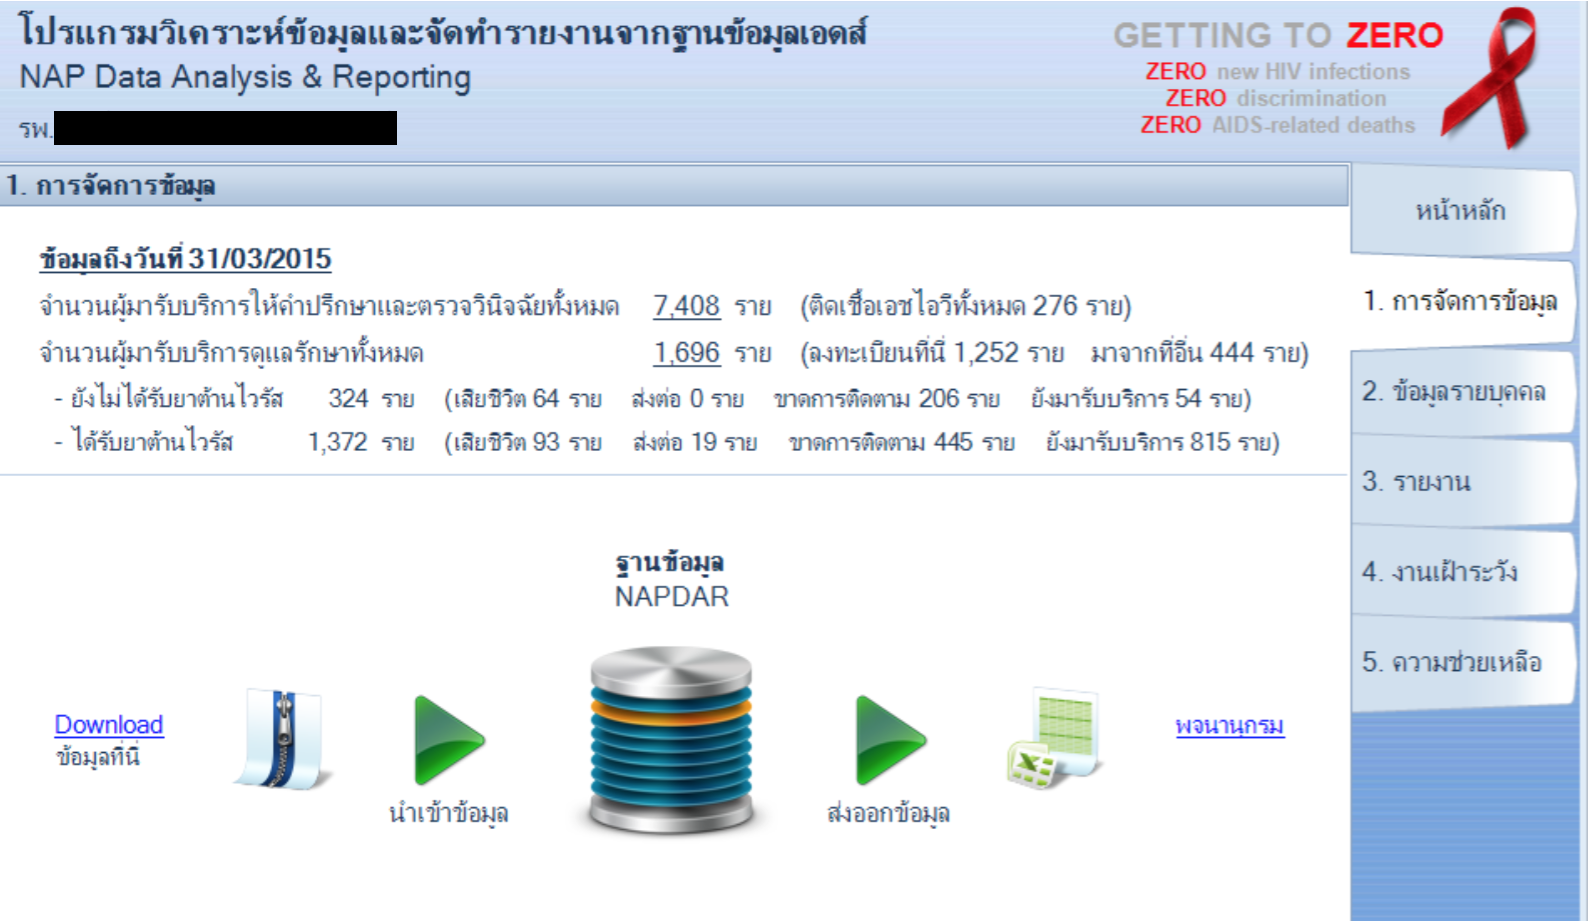
\includegraphics[width=12cm]{images/chapter-01/napdar-01.png}
    		\caption{NAPDAR Data Management Page}
    \end{figure}
\FloatBarrier

\FloatBarrier
	\begin{figure}[h!]
        \centering
    		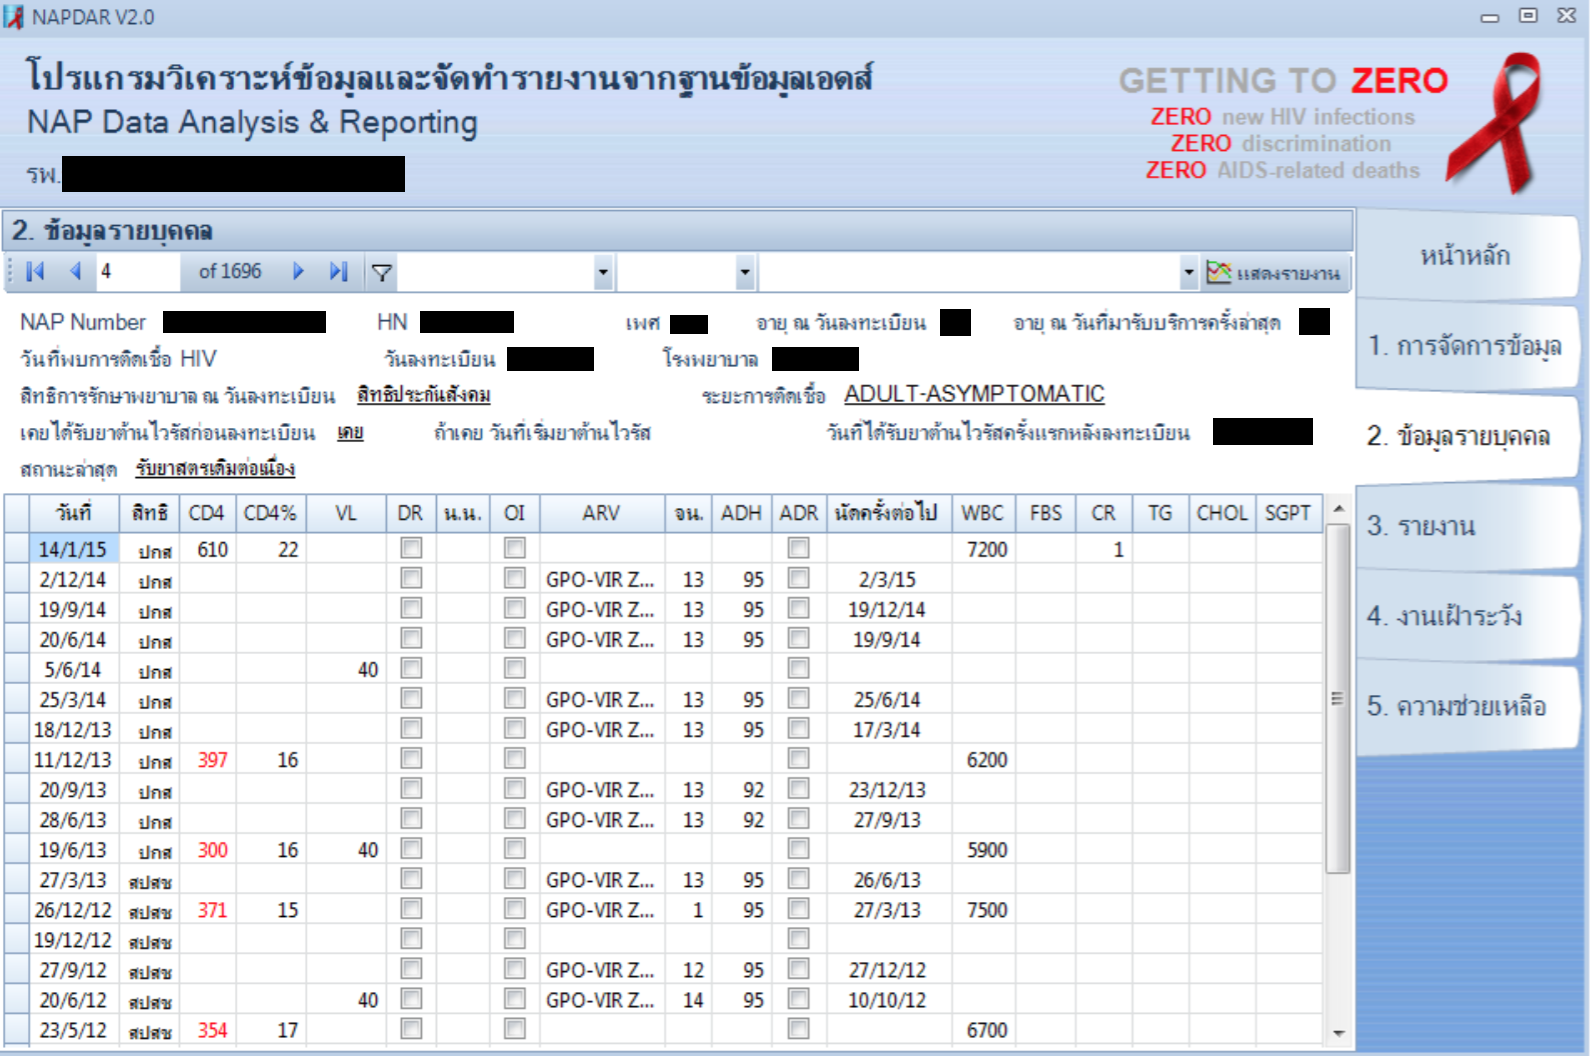
\includegraphics[width=12cm]{images/chapter-01/napdar-02.png}
    		\caption{NAPDAR Individual Report Page}
    \end{figure}
\FloatBarrier

\FloatBarrier
	\begin{figure}[h!]
        \centering
    		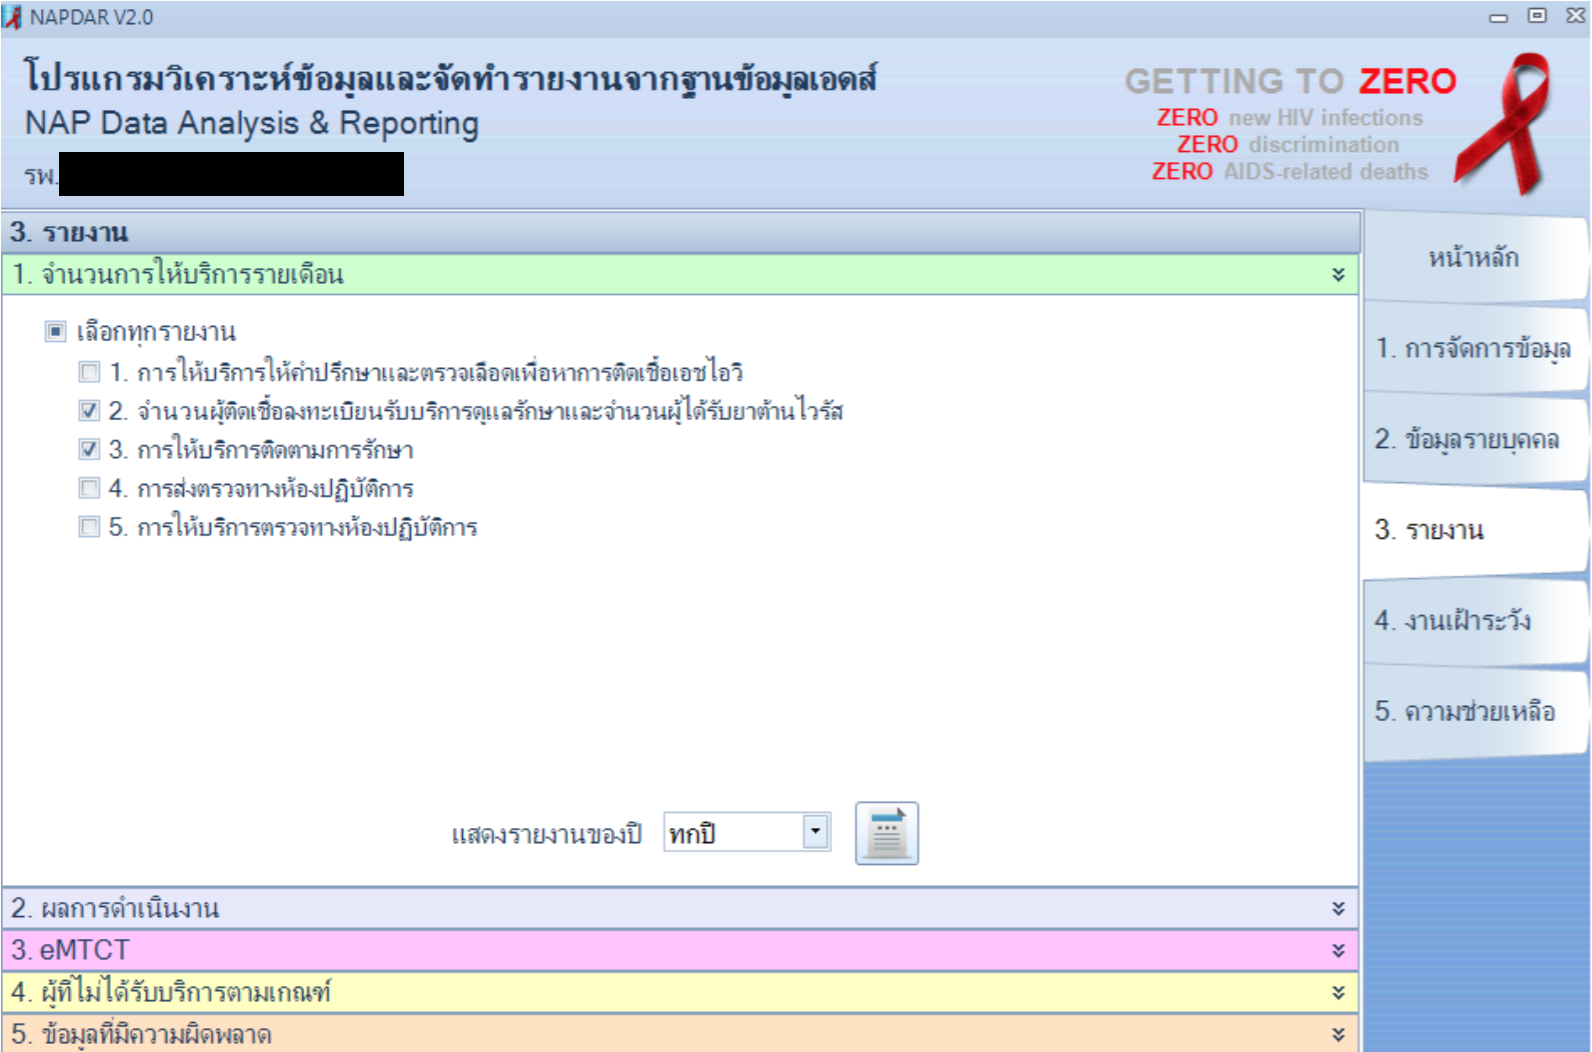
\includegraphics[width=12cm]{images/chapter-01/napdar-03.png}
    		\caption{NAPDAR Generating Monthly Report Page}
    \end{figure}
\FloatBarrier

% \FloatBarrier
% 	\begin{figure}[h!]
%         \centering
%     		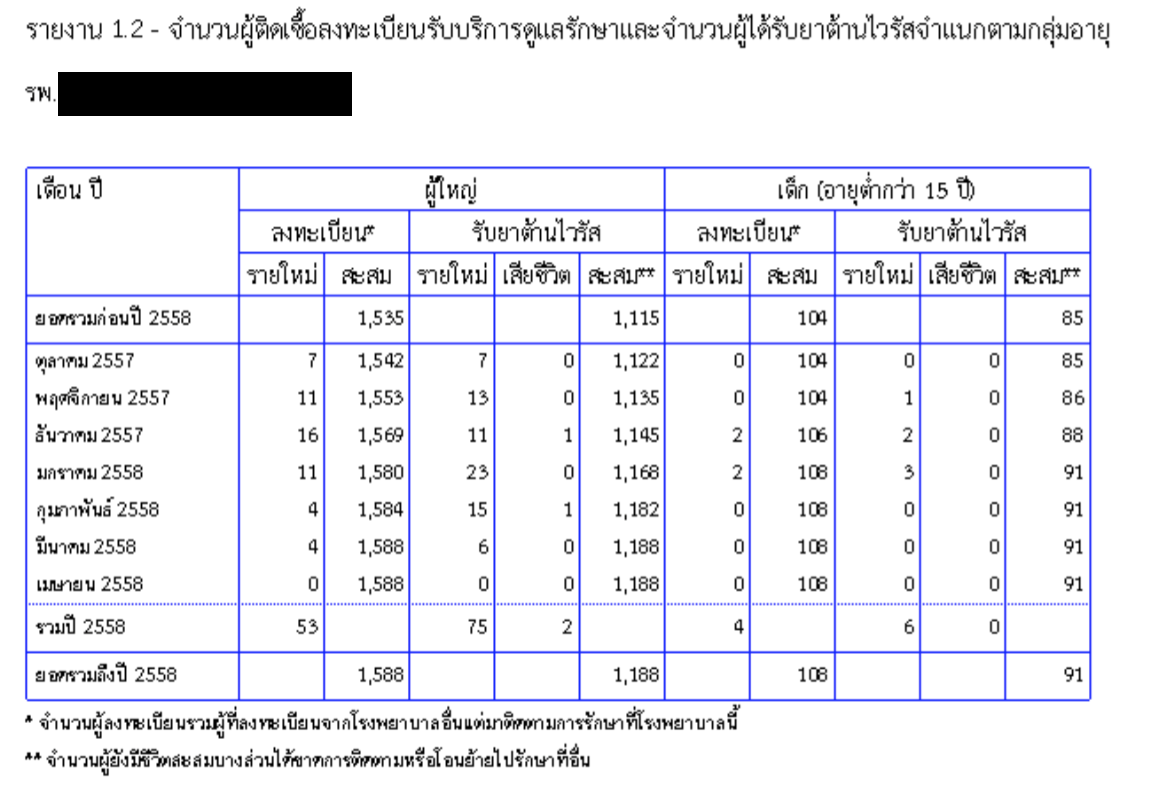
\includegraphics[width=12cm]{images/chapter-01/napdar-04.png}
%     		\caption{NAPDAR Report 1.2}
%     \end{figure}
% \FloatBarrier

\FloatBarrier
	\begin{figure}[h!]
        \centering
    		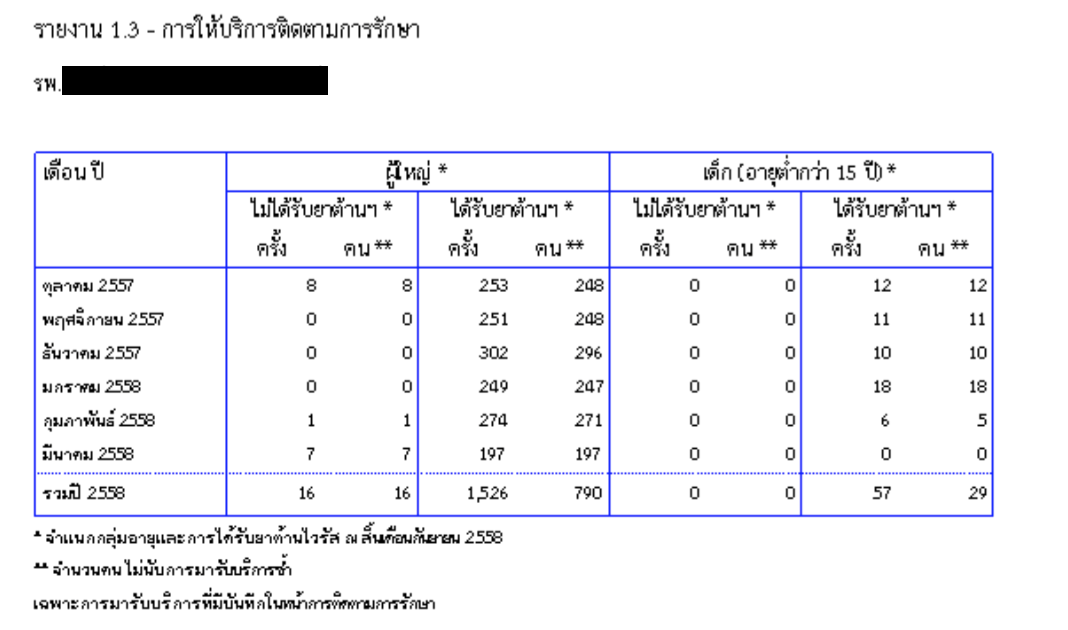
\includegraphics[width=12cm]{images/chapter-01/napdar-05.png}
    		\caption{NAPDAR Follow Up Patient Report}
    \end{figure}
\FloatBarrier

% \FloatBarrier
% 	\begin{figure}[h!]
%         \centering
%     		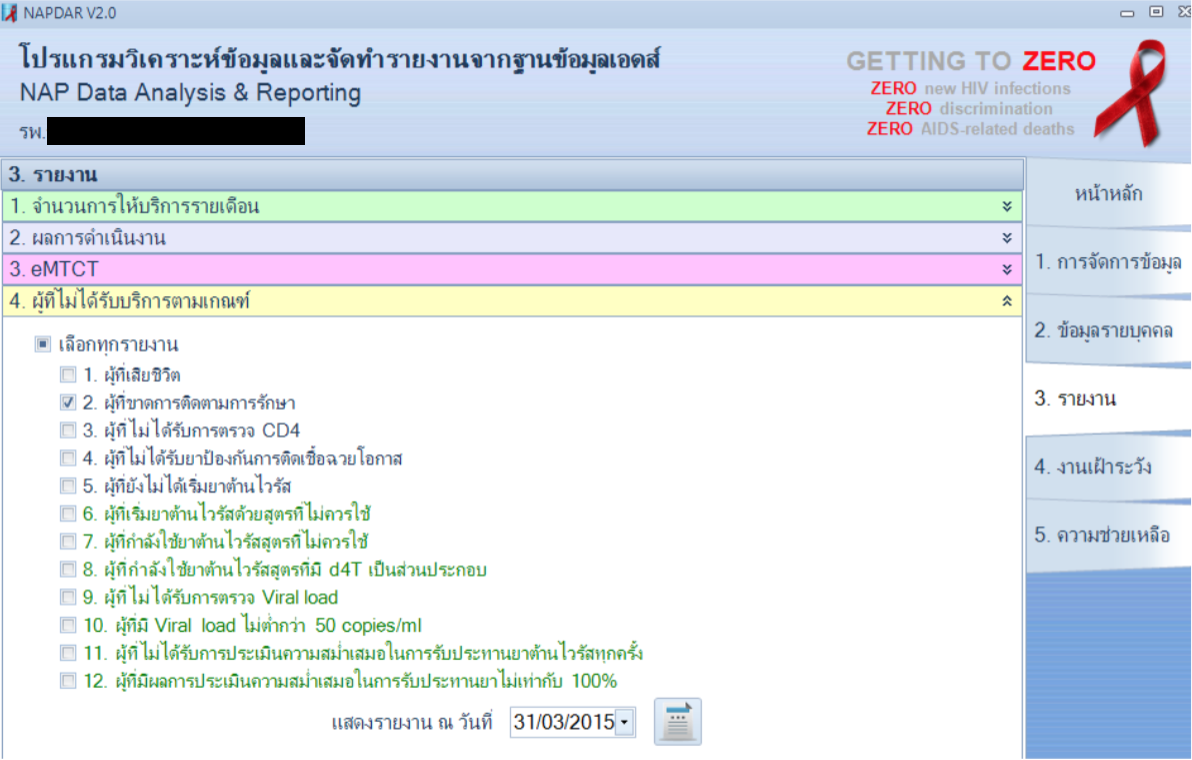
\includegraphics[width=12cm]{images/chapter-01/napdar-06.png}
%     		\caption{NAPDAR Untreated Patient Report Page}
%     \end{figure}
% \FloatBarrier

% \FloatBarrier
% 	\begin{figure}[h!]
%         \centering
%     		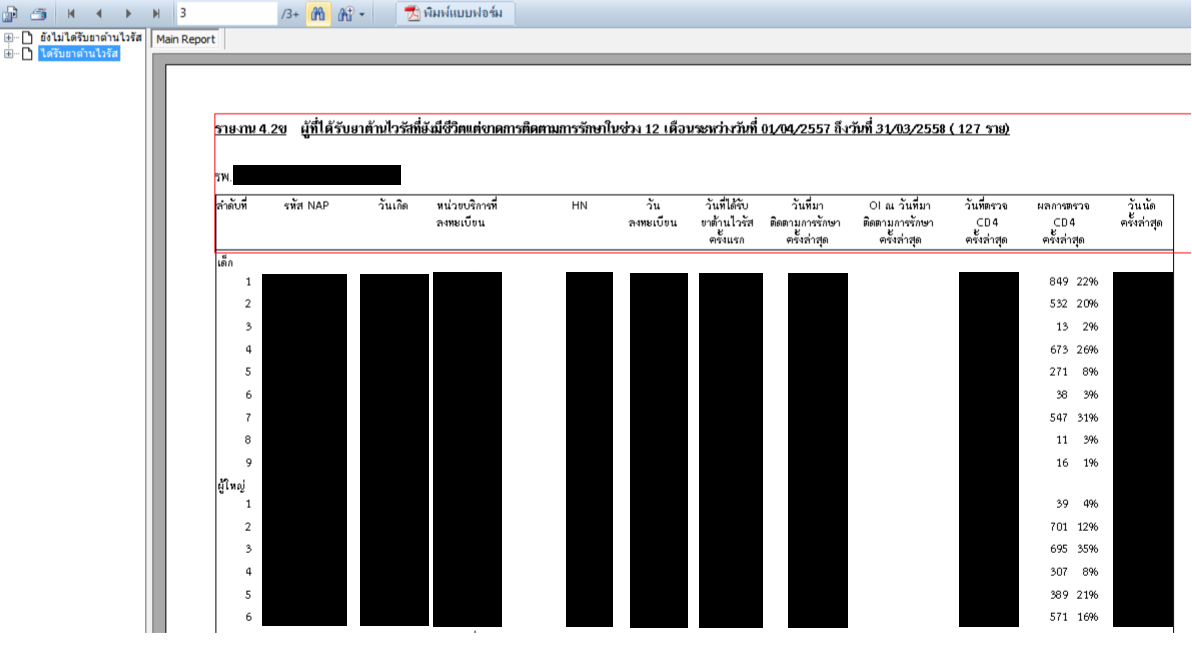
\includegraphics[width=12cm]{images/chapter-01/napdar-07.png}
%     		\caption{NAPDAR Treated Patient with Lost Follow Up Report Page}
%     \end{figure}
% \FloatBarrier

\FloatBarrier
	\begin{figure}[h!]
        \centering
    		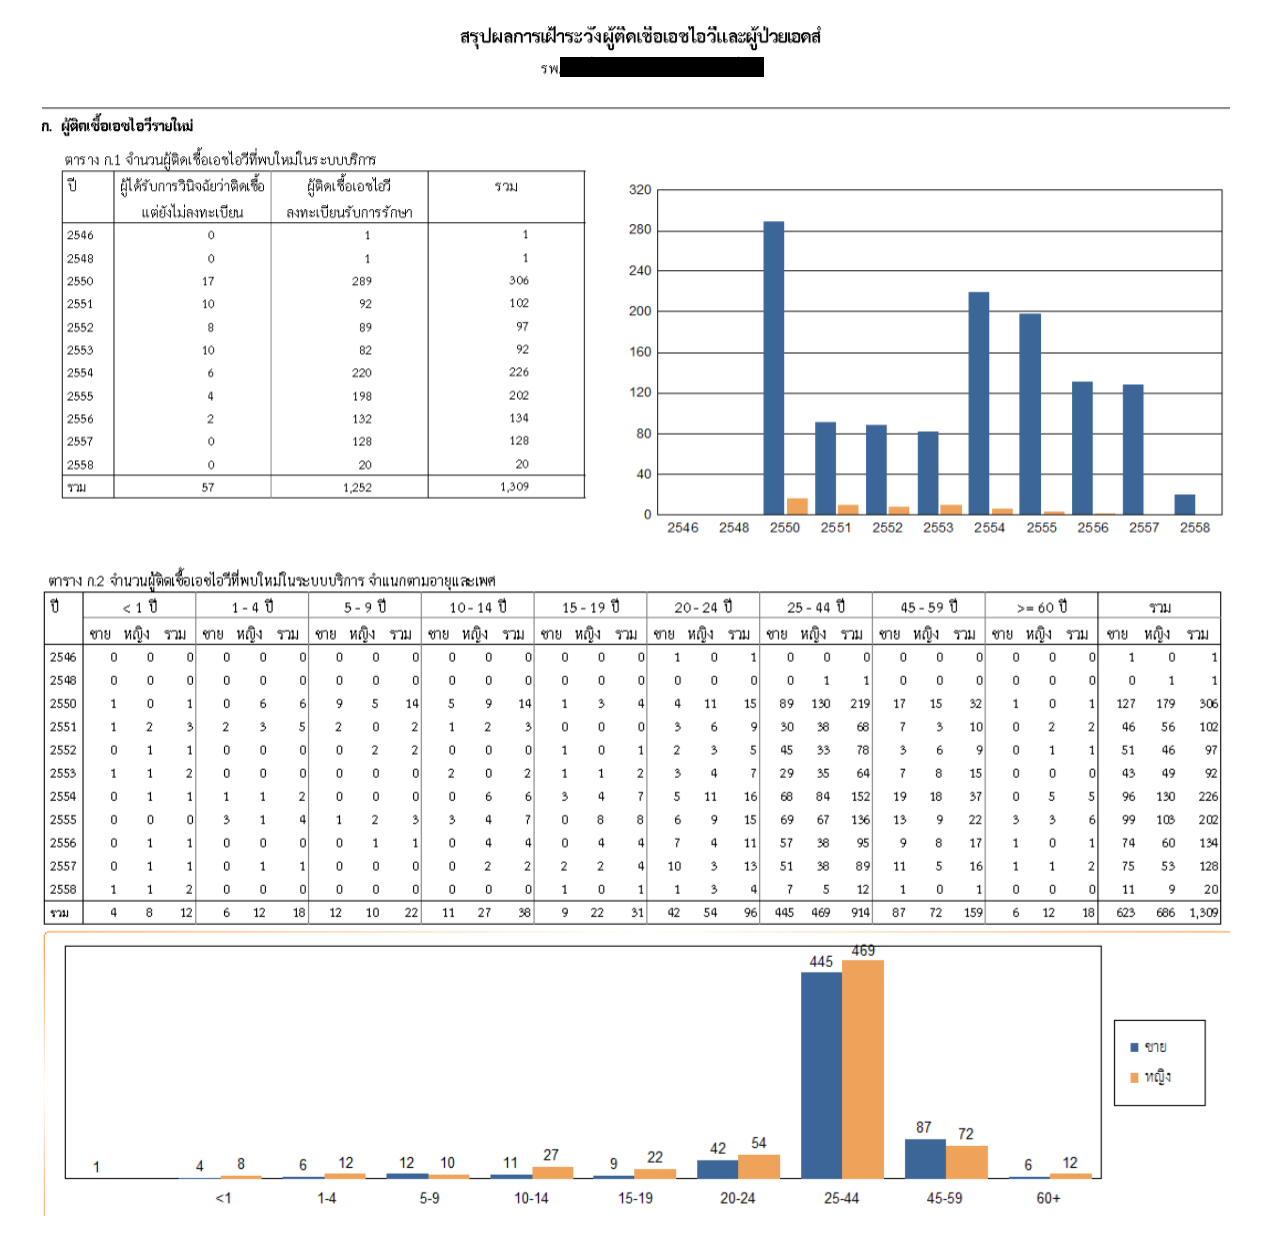
\includegraphics[width=\linewidth]{images/chapter-01/napdar-08.png}
    		\caption{NAPDAR Summary Report Page}
    \end{figure}
\FloatBarrier
	
	There are several limitations of NAP and NAPDAR. First, the data in NAP only include people who register in National Health Security Office. This means, there will be no record from the patient who does not register to National Health Security Office and the foreigners. Since Thailand has lots of foreign worker, they is one of the large portion where the budget of drug has been use. Next, the medical staff needs download each file from NAP and then upload them to NAPDAR in order to generate the report. This gives them more tasks to do. Thirdly, NAPDAR system can analyse and generate the report from the data in hospital level. It cannot generate the report of country level. This means the user of the system will not be able to see the whole picture of the situation.	


\section{Project Scope}
    
    In this project, we are going to create a solution for Bureau of Epidemiology along with other organization such as hospitals, provincial public health offices, organizations under the supervised from Ministry of Public Health (Bureau of AIDS TB and STIs, Bureau of Strategy and Policy, Information Technology and Communication Center, Bureau of Health Promotion, Office of the Permanent Secretary, Department of Medical Science), organizations under Bangkok Metropolitan Administration (Health Department, Medical Service Department), and Thailand MOPH-US CDC Collaboration. The users of the EIIS must be able to interact with the system according to their roles. Our goal is to complete the requirements as mentioned in section \ref{requirements}.

    \chapter{Requirements}

    There are a lot of problems that they are facing, in order to build the system to surveil and follow the patient who have disease under surveillance and make policy decision, we are invited to be in the same team to help the ministry of public health to build Epidemic Intelligent Information System(EIIS). We went to discuss with the team in order to understand the overall situations and gather the requirements. There are six main requirements that they need which are at a glance report, demographics report, lab-upload function, and upload status page, individual report and workload report. 
    
\section{At a glance Report}
    In this requirement, they want the system to show the a glance report page which will show the report that they can surveil and follow the patient in order to control and prevent diseases under surveillance.
    In order to see how at a glance report work, you can see activity diagram in chapter two in  \ref{glance-report}, and also can see the user interface of at a glance report in \ref{at-a-glance-report}.
    % example to see the table

        
\section{Demographics Report}
    In this requirement, they also want a demographics report page that will show the summary of the data that come in to this system. For example nationality pie chart, occupation pie chart, sex pie chart, and so on. The example of the chart is in \ref{demographics_report}. In addition, you can see all the steps in order to see demographics report in chapter two in section \ref{demographics_report_sec}, and also can see the activity diagram in figure \ref{demographics}
        
\section{Upload}
% upload what file?
    Uploading the file is one requirement that they want in this system because they want every hospital can upload file and send to the system. The example of user interface design is show in section \ref{upload_file} in figure between \ref{upload-status1} and \ref{upload-status3} . Furthermore, all the steps to see how to upload is show in section \ref{upload_file_activity_diagram} in figure \ref{upload}

\section{Checking Upload Status}
    Since they want upload function then checking upload status is the require too in order for them to check the status of the uploading file. Checking upload status means that they can check that which month that they are not sending the file, so they can upload the missing file. The example of user interface design is show in section \ref{check_upload_history_status_ui}. Furthermore, all the steps to see how to upload is show in \ref{check_upload_status_activity_diagram}
    
\section{Individual Report}
    In this requirement, they want the system to show the individual report that will they can see the report of each patient in their hospital. Only that disease coordinator in each hospital can see their own patient individual report. From this report they want to check whether the patient still receive drug or not and where the patient are. This will help them to keep track of the patient even thought the patient went to another hospital but his/her is still alive. Moreover, they also want to see the status of the patient where the condition of the disease are getting worse or better from the level of CD4 and viral load. Furthermore, all the steps to see individual report is show in \ref{individual_report_activity_diagram}
    
\section{Workload Report}
    Workload report is one of requirement that they want the system to be able to show.This report need to be able to show how many patient who come to hospital in certain diseases of choosing period of time. The reason they want this report is to minimise and maximise the workload they will have in the future and to be able to estimate the budget need to invest in the drug.Furthermore, all the steps to see workload report is show in \ref{workload_report_activity_diagram}
    \chapter{System Analysis and Design}

\section{Architecture Overview}
    This project's architecture is designed not only to be flexible, but also to maximize the performance result. There are three components in this project; server side, client side, and the database. The client side is the web browser. The server side provides API service for the client side and also connects to the database which is MongoDB in this case.
    
    \vspace{25mm}
    \FloatBarrier
    	\begin{figure}[h!]
            \centering
                % can use width=\linewidth
        		\includegraphics[width=10cm]{images/chapter-03/architecture.png}
        		\caption{Architecture Overview}
        \end{figure}
	\FloatBarrier

\clearpage
\section{Use Case Diagram}
    % only super admin can see individual
    % uploader = can upload
    %user = 
    %hiv coordinator = can see individual only their hosp
    
    We have been gathering requirements from ministry of public health team, we found that there are four main types of user which are super admin, user, HIV coordinator, and up-loader. 
    
    User can log-in to EIIS system, by filling user-name and password, and log-out. User role can see at a glance report, demographics report, upload status page and workload report as shown in figure \ref{use-case}.
    
    
    Super admin can can do everything that User can do, and also see all the individual report which it contains the sensitive information of the patient. For example, id, hospital number codes of the patient, and so on as shown in figure \ref{use-case}. 
    
    
    \FloatBarrier
    	\begin{figure}[h!]
            \centering
                % can use width=\linewidth
        		\includegraphics[width=12cm]{images/chapter-03/UseCaseDiagram.png}
        		\caption{Use Case Diagram}
        		\label{use-case}
        \end{figure}
	\FloatBarrier
	
	Like super admin, HIV coordinator can see the individual report, but they can see only the individual report of their responsibility hospitals. It means that they can see only a group of patient that have a record on that hospital. Unlike other roles, uploader can upload file in and file out to this web-application as shown in figure \ref{use-case2}.
	
	\vspace{15mm}
	\FloatBarrier
    	\begin{figure}[h!]
            \centering
                % can use width=\linewidth
        		\includegraphics[width=12cm]{images/chapter-03/UseCaseDiagram2.png}
        		\caption{Use Case Diagram}
        		\label{use-case2}
        \end{figure}
	\FloatBarrier
	
\clearpage
\section{Activity Diagram}

    \subsection{Log-In}
    % Log-in
    All users role can log in to the EIIS system. All processes to log in are simple. First, they need to fill in user name and password as it shown in figure \ref{log-in}, and after they finish fill in, they just click log-in in order to log-in. If the process is success, it will bring you to the system. If the process is failure, it will warn you that you put the wrong user name or password. The steps of logging-in is shown in figure \ref{log-in-activity-diagram}. 

    \vspace{10mm}
    \FloatBarrier
    	\begin{figure}[h!]
            \centering
                % can use width=\linewidth
        		\includegraphics[width=9cm]{images/chapter-03/logIn_logOut.png}
        		\caption{Log-In}
        		\label{log-in-activity-diagram}
        \end{figure}
	\FloatBarrier
	%Upload
	
	
	\subsection{Upload} \label{upload_file_activity_diagram}
	Only uploader role can upload the file to the system. There are two main steps to upload the file. First, uploader need to choose hospital, month, and year, then click confirm to go to the next step as it shown in figure \ref{upload-status1}. Second, uploader need to choose either file-in or file-out then click upload. If upload process is success, then the upload process is end. If upload process is failure, then uploader have to make sure that they have to choose either file-in or file-out in order to upload as it shown in figure \ref{upload-status2}. If upload fail, it will warn the user as it shown in figure \ref{upload-error}. The steps of uploading is shown in figure \ref{activity_upload}.
	
	\FloatBarrier
    	\begin{figure}[h!]
            \centering
                % can use width=\linewidth
        		\includegraphics[width=6cm]{images/chapter-03/Upload.png}
        		\caption{Upload}
        		\label{activity_upload}
        \end{figure}
	\FloatBarrier
	
	%check upload status
	\subsection{Checking Upload Status} \label{check_upload_status_activity_diagram}
	All users can check the upload status. The steps to check upload status is simple as log-in. First, user need to choose type of report, area, province, and year then click search to see the upload status as it shown in figure \ref{upload-status0}. The steps of checking upload status is shown in figure \ref{check-upload-status}.
	
	\FloatBarrier
    	\begin{figure}[h!]
            \centering
                % can use width=\linewidth
        		\includegraphics[width=10cm]{images/chapter-03/Upload_status.png}
        		\caption{Check Upload Status}
        		\label{check-upload-status}
        \end{figure}
	\FloatBarrier
	
	%At a Glance Report
	\subsection{At a Glance Report} \label{at_a_glance_report}
	All users can see a glance report, and the process to see the report is not complex as in figure \ref{glance-report}. In order to see the report, user need to choose disease, criteria of that disease, times , and types of report area as it shown in figure \ref{at-a-glance-report}. There are three types of time that user can choose which are all time, range time, and end-point. If user select all time, it means that user select the time from the beginning to the end of the data. If user select range time, it means that user need to select the beginning month and year and the end month and year time by themselves. If the user select end-point time, it means that user need to select the endpoint month and year time. In addition, there are four scope of choosing type of report which are all, area, province, and hospital. In this field, if user choose all scope, it means all the data. If user choose area scope, it means that user have to choose specific area. Like area, if user choose province scope, it means that user have to choose specific area first then it will filter the provinces of that area, and user need to choose province. If user choose hospital scope, then user need to choose area, province, and hospital. If you want to see all the select user interface, you can see in section \ref{filter-data}. The steps of requesting at a glance report is shown in figure \ref{glance-report}
	
	\FloatBarrier
    	\begin{figure}[h!]
            \centering
                % can use width=\linewidth
        		\includegraphics[width=\linewidth]{images/chapter-03/atAGlance.png}
        		\caption{At a Glance Report}
        		\label{glance-report}
        \end{figure}
	\FloatBarrier
	
	%Demographics Report
	\subsection{Demographics Report} \label{demographics_report_sec}
	All users can see a demographics report, and the process is close to the process to see a glance report as the user interface of demographics report is shown in figure \ref{demographics-report}. In order to see the report, user need to choose nation, disease, criteria of that disease, times , and types of report area.There are three types of time that user can choose which are all time, range time, and end-point. If user select all time, it means that user select the time from the beginning to the end of the data. If user select range time, it means that user need to select the beginning month and year and the end month and year time by themselves. If the user select end-point time, it means that user need to select the endpoint month and year time. In addition, there are four scope of choosing type of report which are all, area, province, and hospital. In this field, if user choose all scope, it means all the data. If user choose area scope, it means that user have to choose specific area. Like area, if user choose province scope, it means that user have to choose specific area first then it will filter the provinces of that area, and user need to choose province. If user choose hospital scope, then user need to choose area, province, and hospital. If you want to see all the select user interface, you can see in section \ref{filter-data}. The steps of requesting demographics report is shown in figure \ref{demographics}
	
	
	 \FloatBarrier
    	\begin{figure}[h!]
            \centering
                % can use width=\linewidth
        		\includegraphics[width=\linewidth]{images/chapter-03/Demographics.png}
        		\caption{Demographics Report}
        		\label{demographics}
        \end{figure}
	\FloatBarrier
	
	%Individual Report
 	\subsection{Individual Report}
 	\label{individual_report_activity_diagram}
 	Only HIV coordinator and super admin roles that can view individual report. There is only 1 main step in order to see individual patient information. That step is to click "see information" at the last column of that row that contain the CID of the patient you want to view their information. Moreover, at the first page of individual report it can only contain 50 patients, so there will be previous and next bottom for look up the rest of patients. At individual report there is also a back button where you can click and go back to first step in order to look at another individual patient information. The steps of requesting individual report is shown in figure \ref{individual-report} However, for the user interface is the work that we will reimplemented in the future.
 	
 	\FloatBarrier
     	\begin{figure}[h!]
            \centering
                 % can use width=\linewidth
         		\includegraphics[width=9cm]{images/chapter-03/individual_report.png}
         		\caption{Individual Report}
        		\label{individual-report}
        \end{figure}
 	\FloatBarrier

	%Workload Report
 	\subsection{Workload Report}
 	\label{workload_report_activity_diagram}
 	All users can see a workload report, and the process is close to the process of how to see demographic report except there is no choosing the criteria. In order to see the report, user need to choose disease, times, nation and types of report area. There are three types of time that user can choose which are all time, range time, and end-point as same as demographic report or at a glance report. In addition, there are four scope of choosing type of report which are all, area, province, and hospital. In this field, if user choose all scope, it means all the data. If user choose area scope, it means that user have to choose specific area. Like area, if user choose province scope, it means that user have to choose specific area first then it will filter the provinces of that area, and user need to choose province. If user choose hospital scope, then user need to choose area, province, and hospital. The steps of requesting workload report is shown in figure \ref{workload-report} However, for the user interface of workload report is the work that we will reimplemented in the future.
 	
 	\FloatBarrier
     	\begin{figure}[h!]
            \centering
                 % can use width=\linewidth
         		\includegraphics[width=14cm]{images/chapter-03/workload_report.png}
         		\caption{Workload Report}
        		\label{workload-report}
        \end{figure}
 	\FloatBarrier

\vspace{10mm}
\section{User Interface Design}
    At the beginning of the project the requirement of user interface of the system is not stable, so we design to create a mock-up user interface to show them that how the system should look like by using draw.io. After that we design to create the mock up system using ruby on rails to show the work flow of the system.
    

    % ????? do we need to separate draw.io into two pic?
    % % should we seperate it into 2 pic
\chapter{User Interface Design}

    \section{Draw.io}
        \FloatBarrier
            \begin{figure}[h!]
                \centering
                    \includegraphics[width=12cm]{images/chapter-01/Mockup_Ui_CDC_final_overall.png}
                	\caption{Mock Up User Interface Using Draw.io}
                	\label{fig_mock_draw_io}
            \end{figure}
        \FloatBarrier
        
    \section{Ruby on Rails Mock Up} \label{ruby_on_rails_mock_up}
            \FloatBarrier
                \begin{figure}[h!]
                    \centering
                        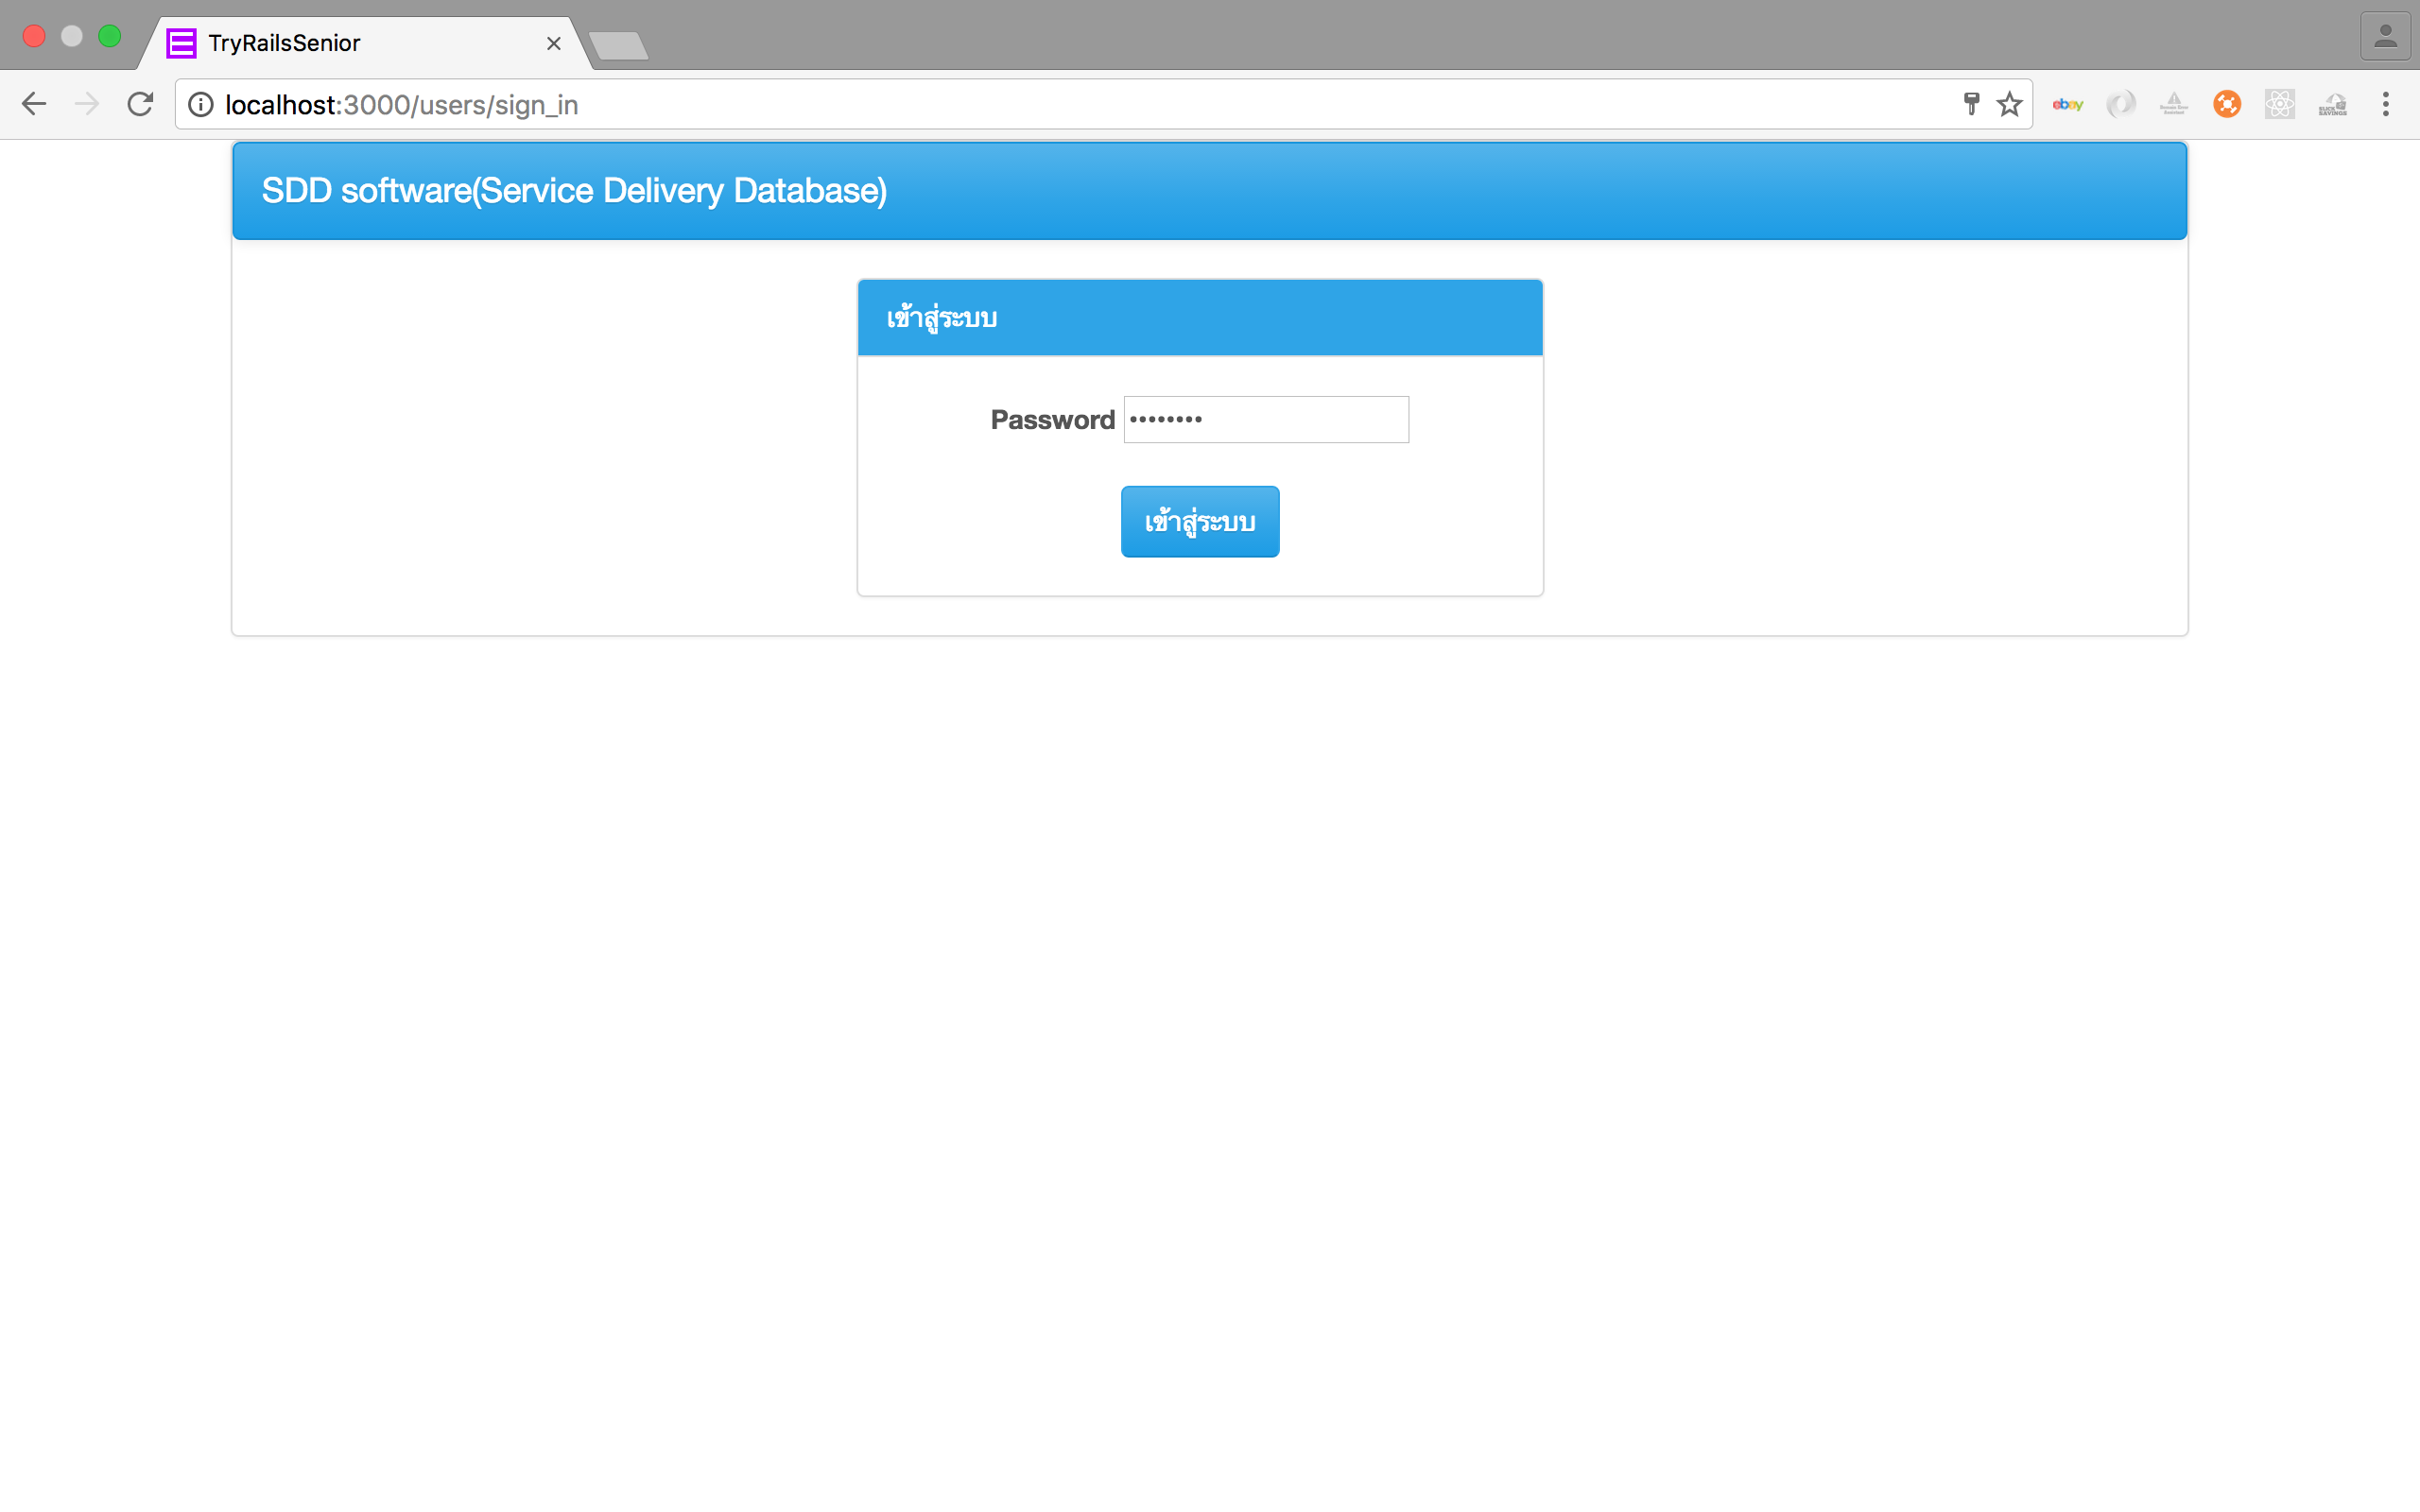
\includegraphics[width=12cm]{images/chapter-01/mockup_rails/log_in.png}
                    	\caption{Log-In Page}
                    	\label{log_in}
                \end{figure}
            \FloatBarrier
            
            \FloatBarrier
                \begin{figure}[h!]
                    \centering
                        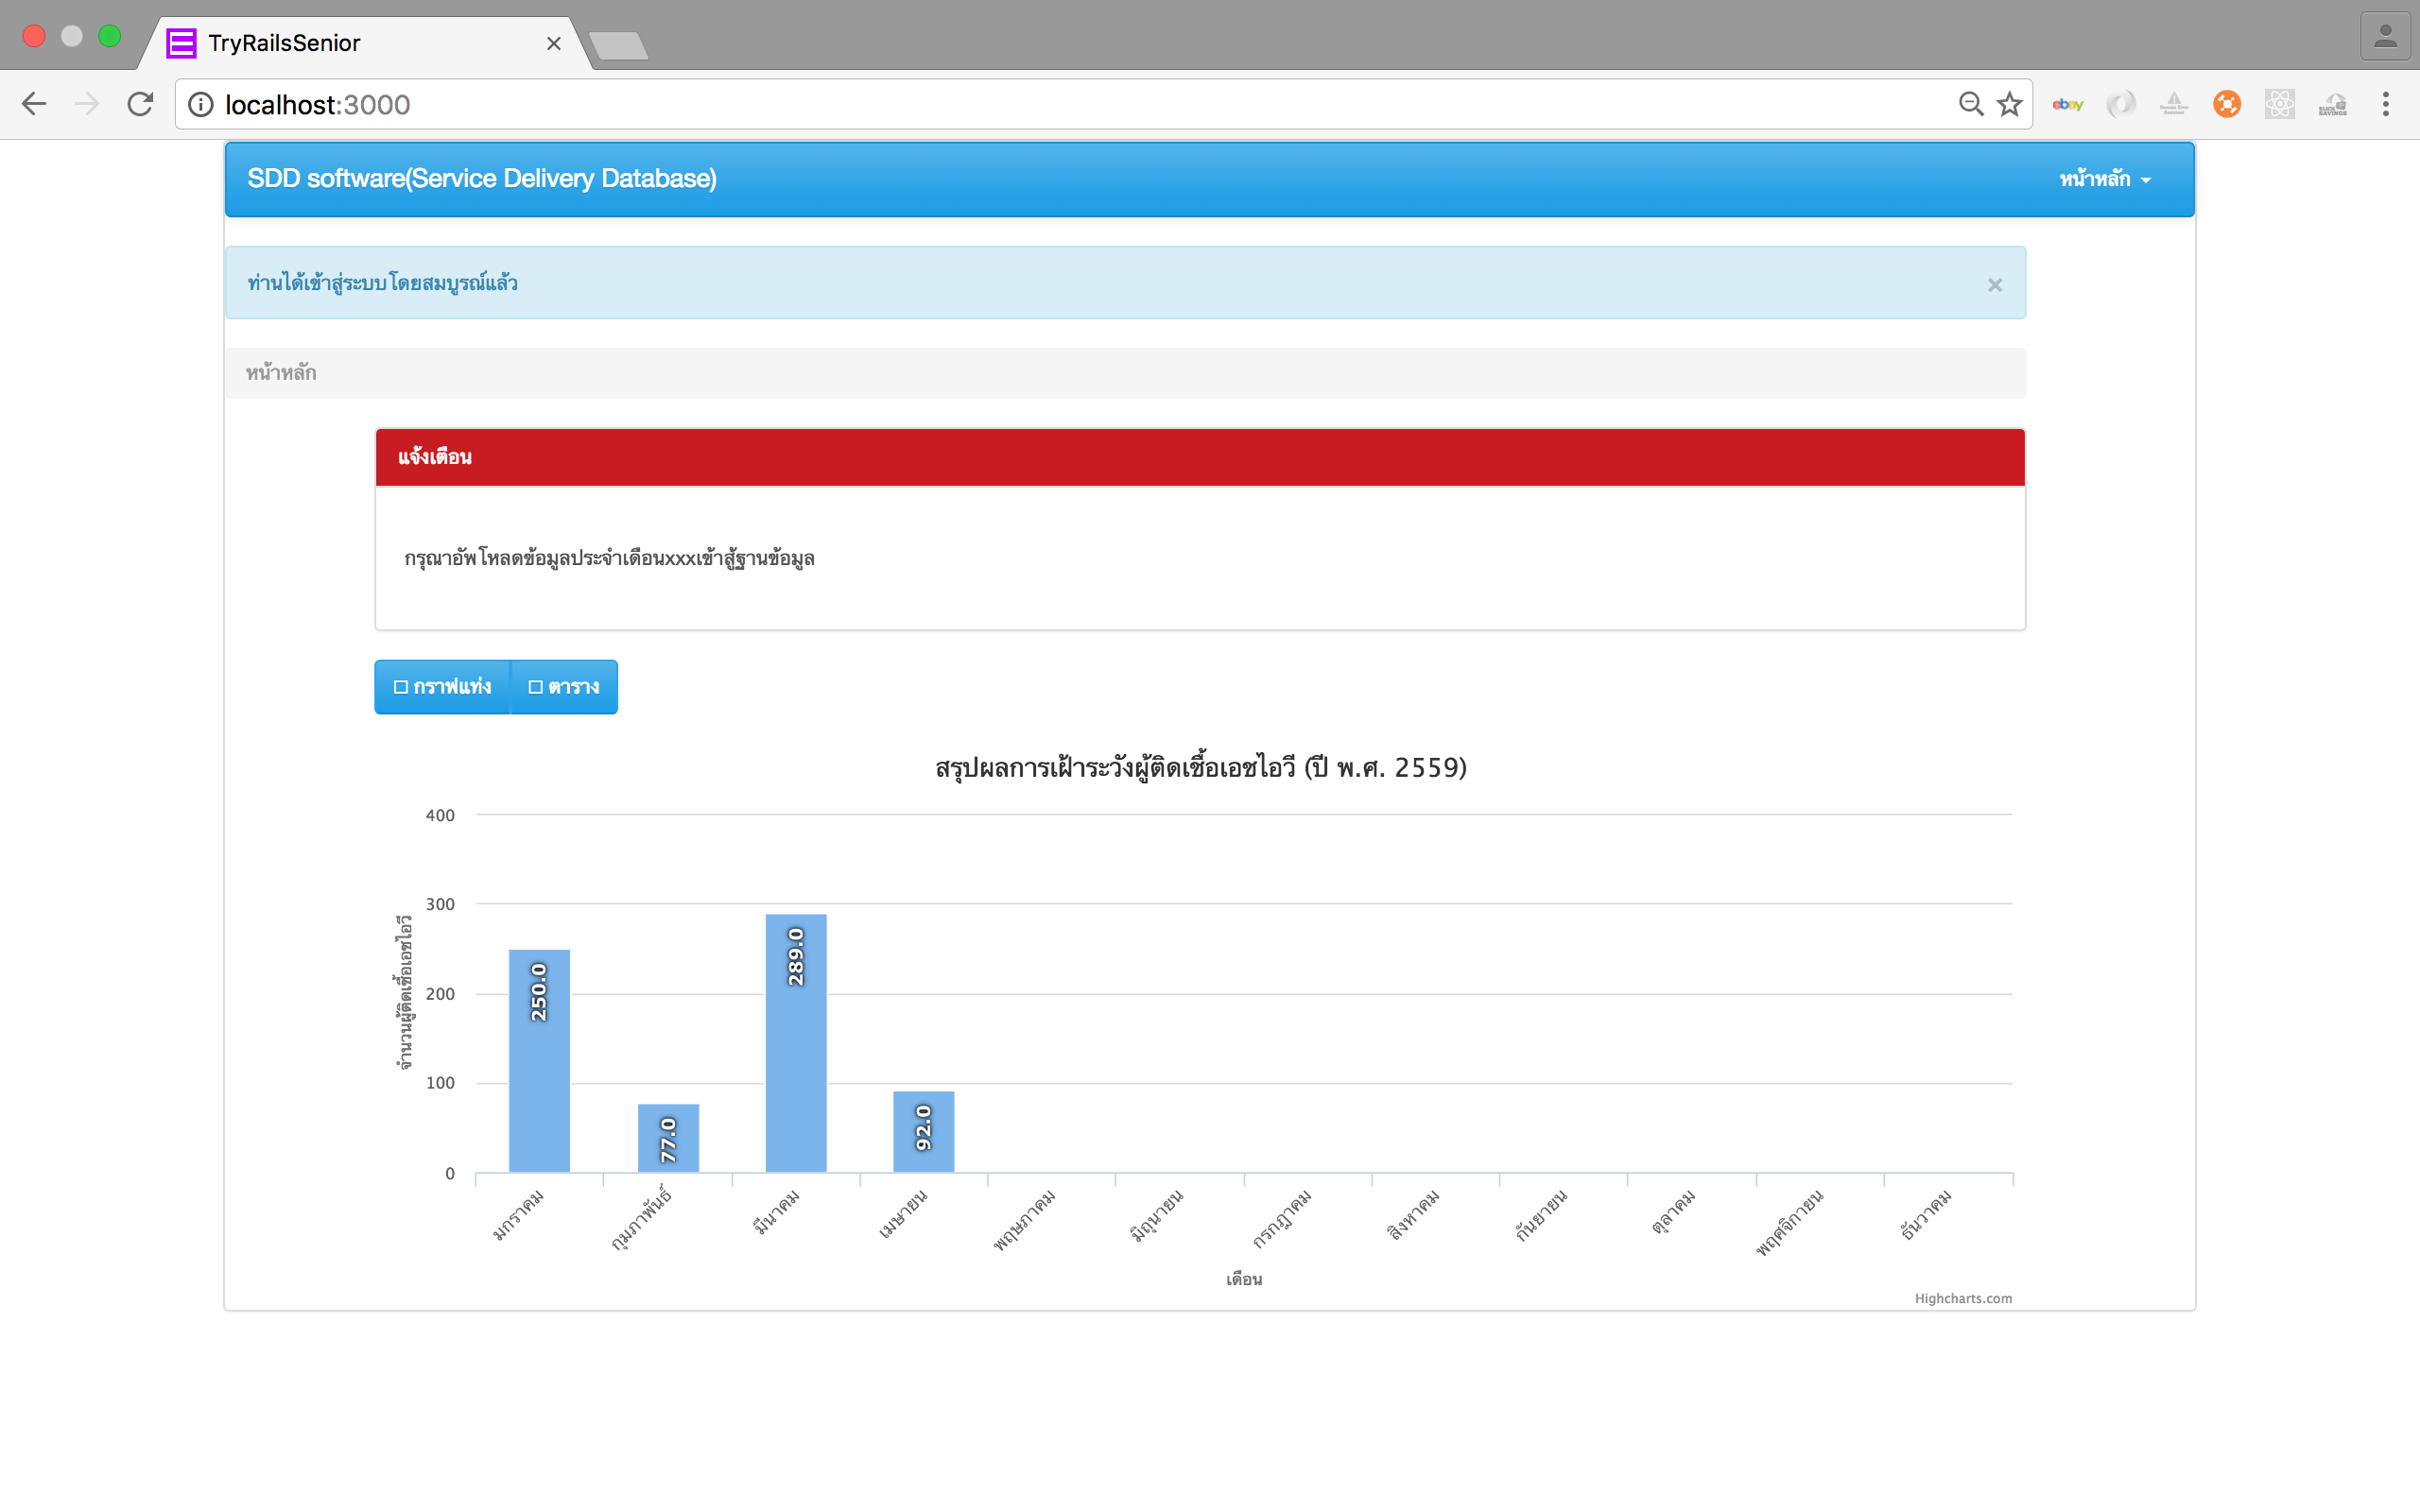
\includegraphics[width=12cm]{images/chapter-01/mockup_rails/home.png}
                    	\caption{Home Page}
                    	\label{home}
                \end{figure}
            \FloatBarrier
            
            \FloatBarrier
                \begin{figure}[h!]
                    \centering
                        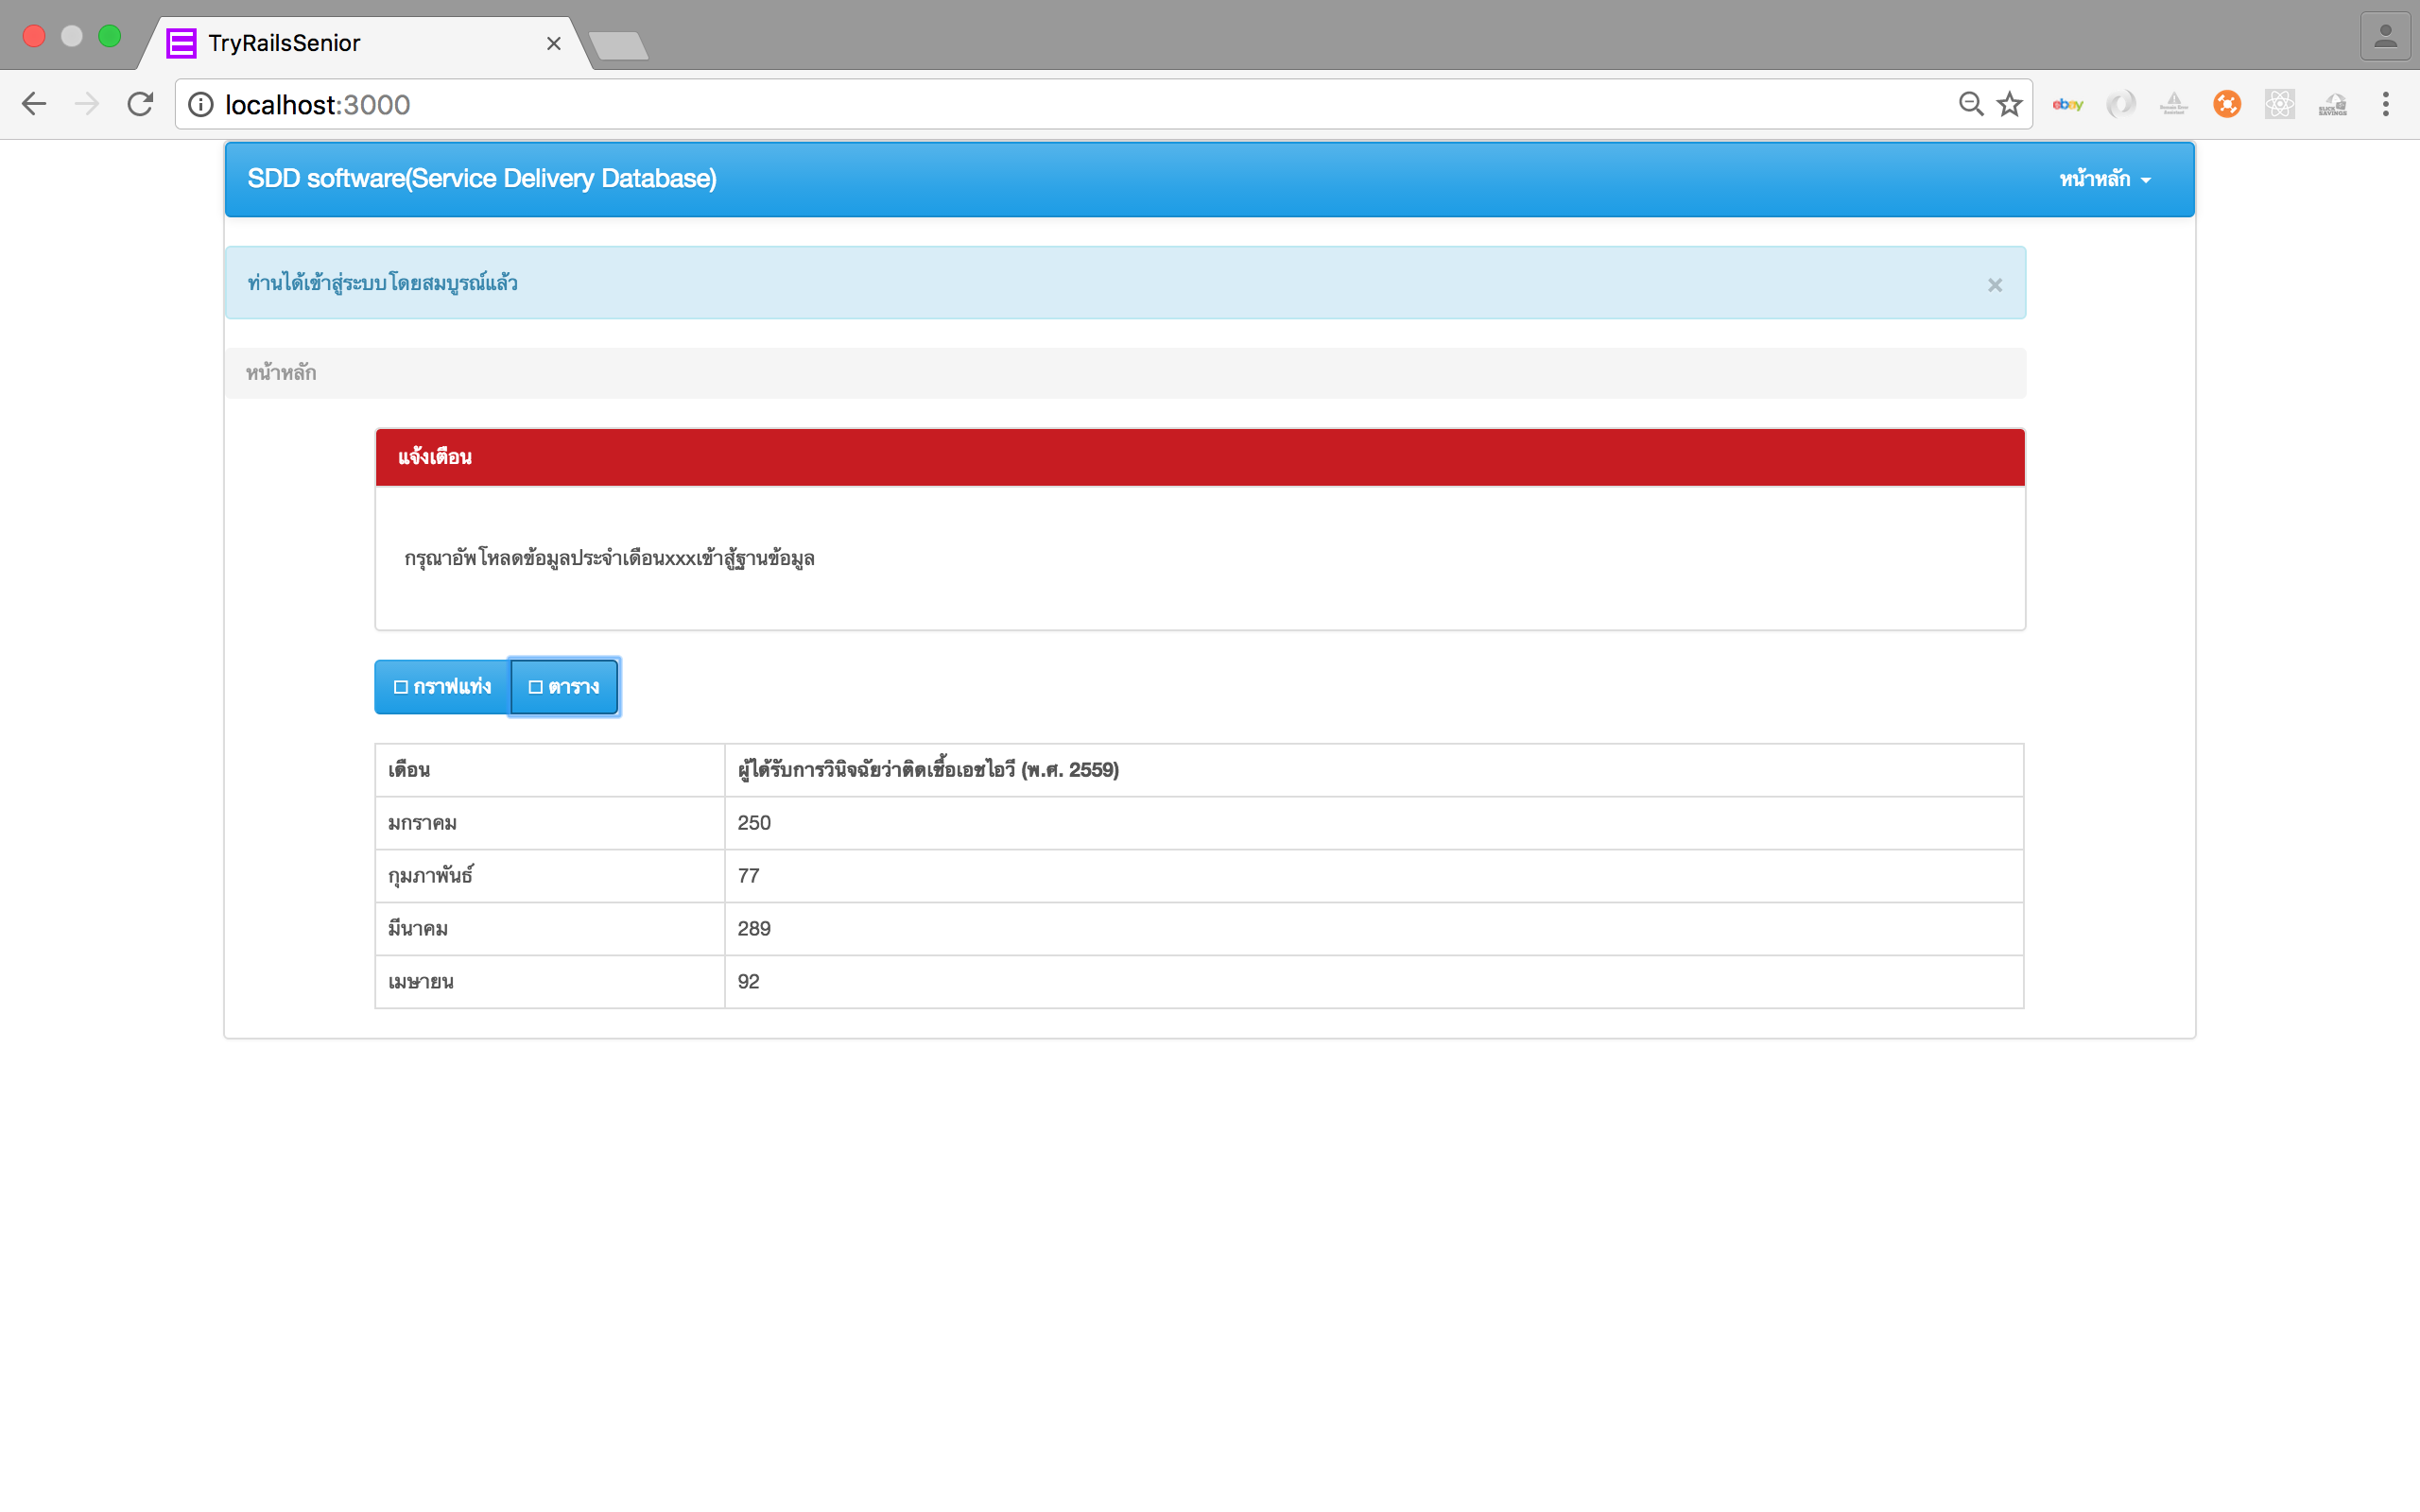
\includegraphics[width=12cm]{images/chapter-01/mockup_rails/home2.png}
                    	\caption{Home Page2}
                    	\label{home2}
                \end{figure}
            \FloatBarrier
        
            \FloatBarrier
                \begin{figure}[h!]
                    \centering
                        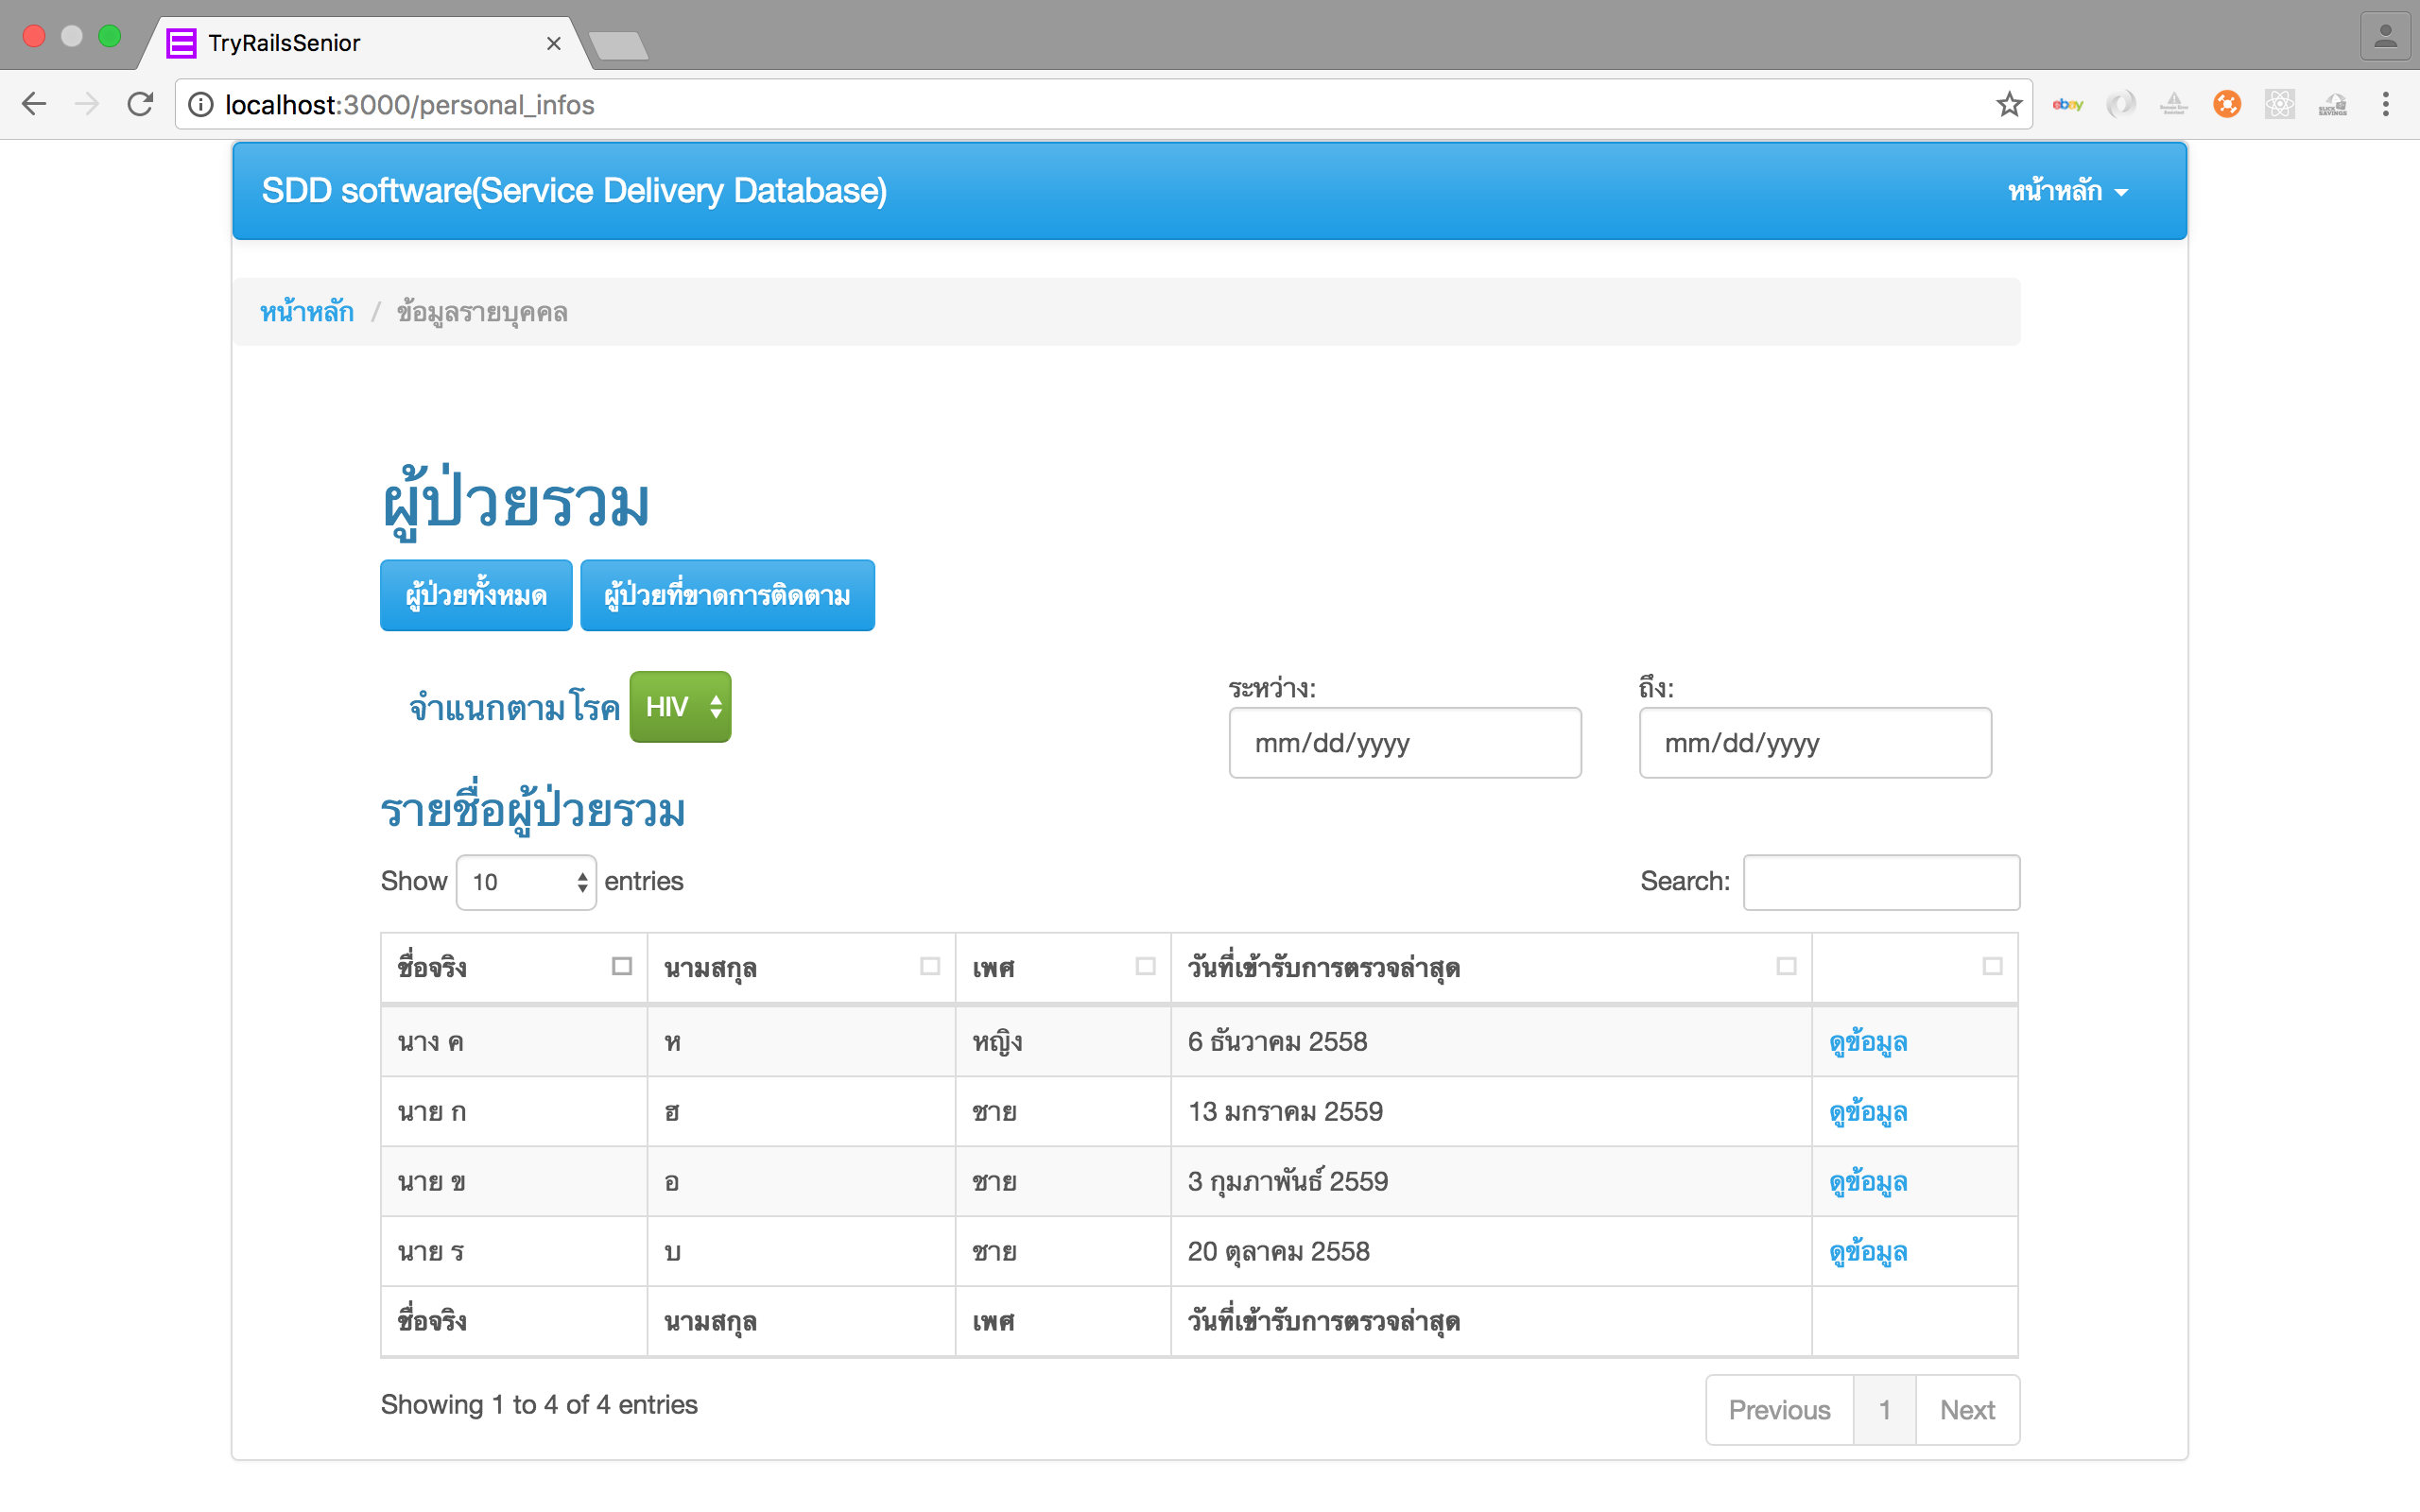
\includegraphics[width=12cm]{images/chapter-01/mockup_rails/individual_report.png}
                    	\caption{Individual Report Table}
                    	\label{individual_report}
                \end{figure}
            \FloatBarrier
            \FloatBarrier
                \begin{figure}[h!]
                    \centering
                        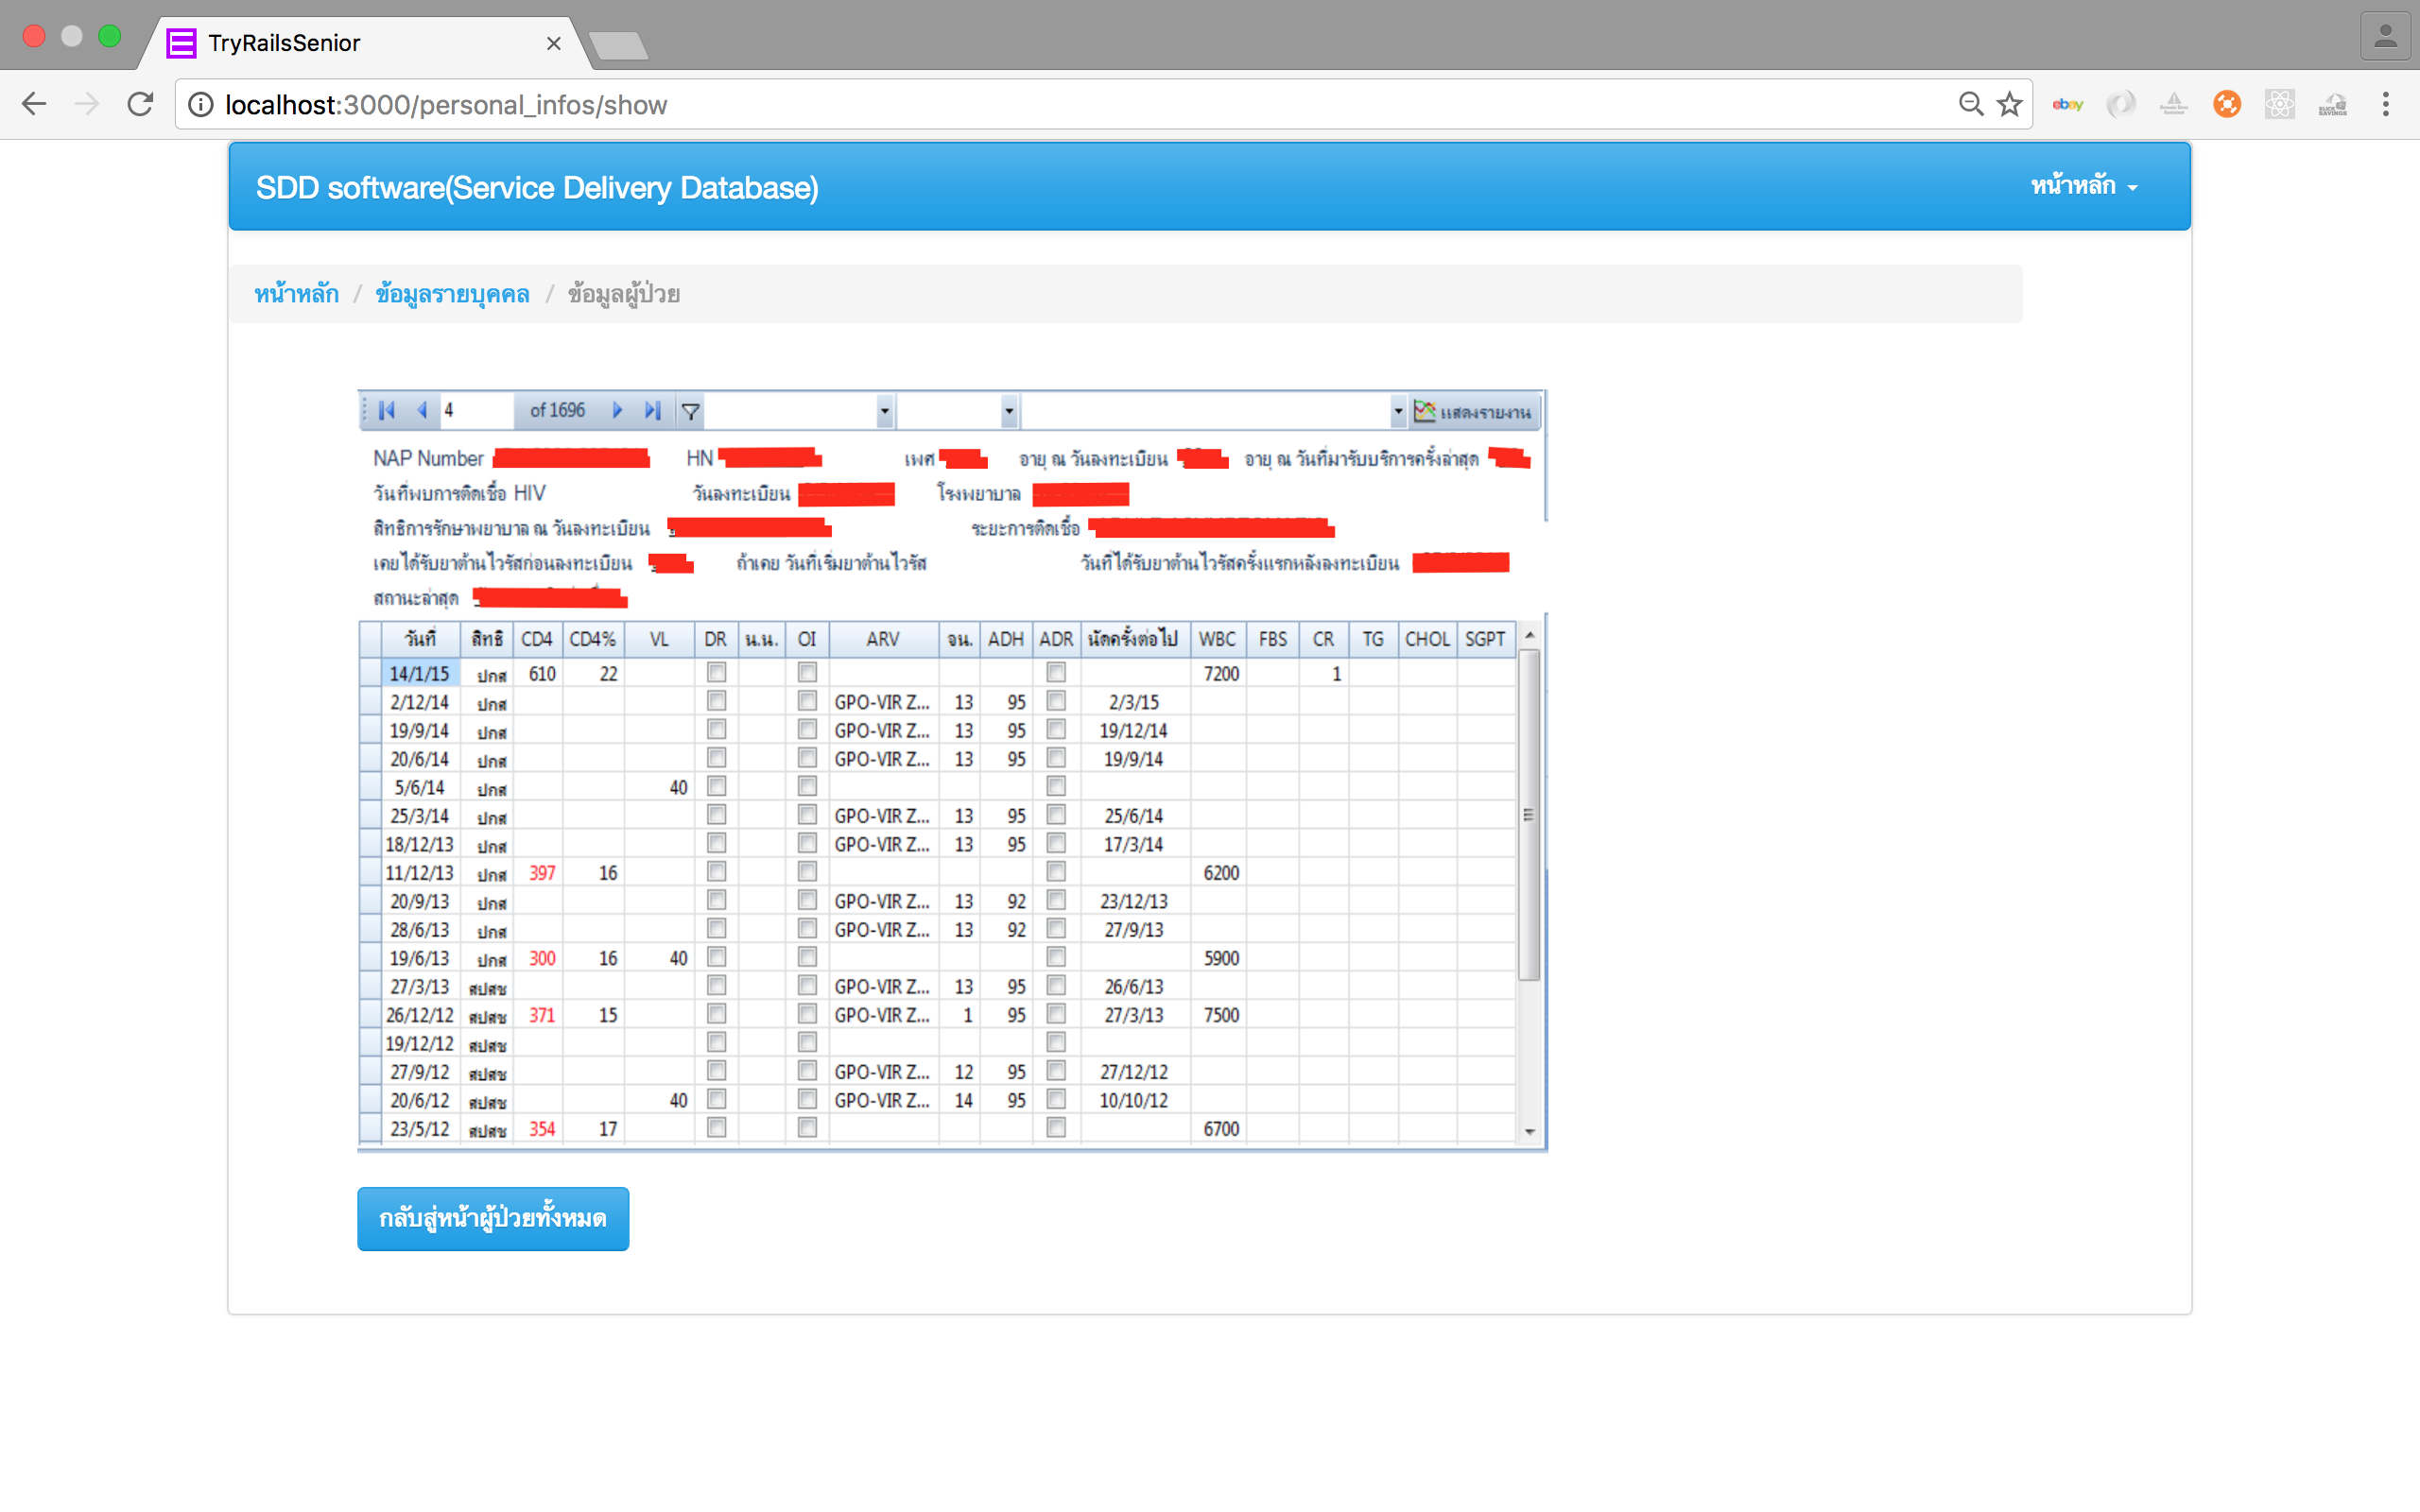
\includegraphics[width=12cm]{images/chapter-01/mockup_rails/individual_report1.png}
                    	\caption{Individual Report Details}
                    	\label{individual_report1}
                \end{figure}
            \FloatBarrier
            
            \FloatBarrier
                \begin{figure}[h!]
                    \centering
                        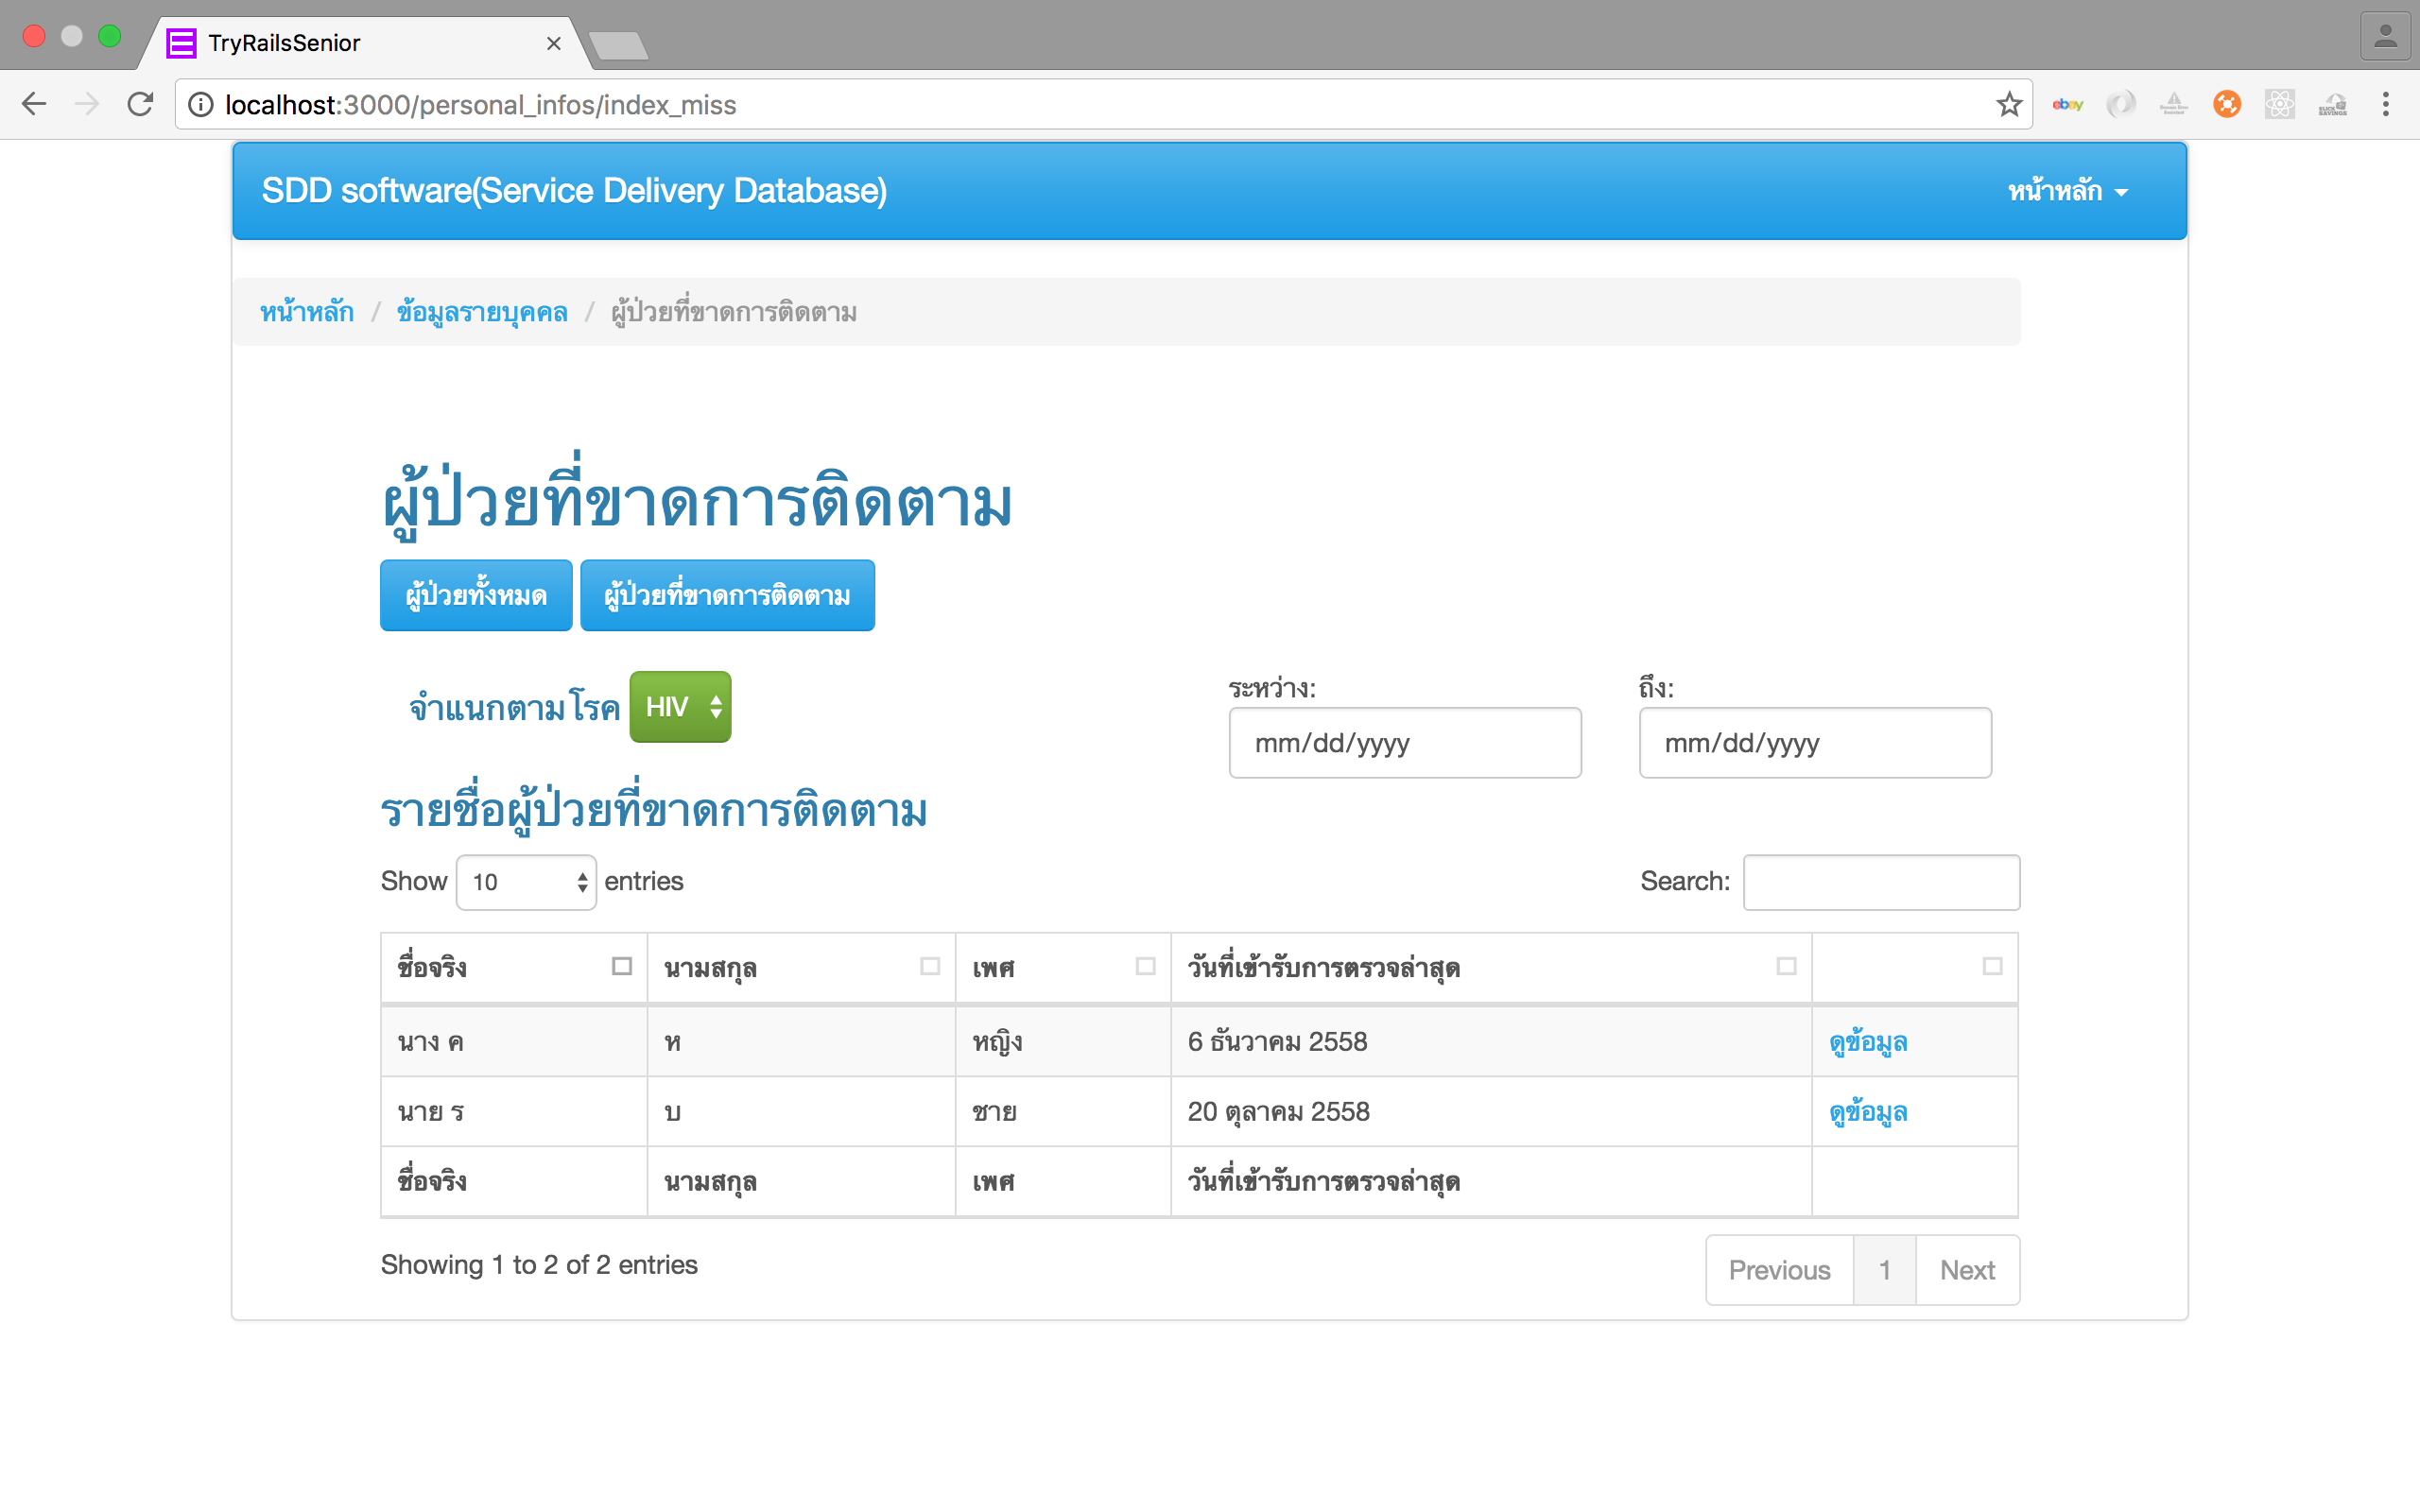
\includegraphics[width=12cm]{images/chapter-01/mockup_rails/lost_follow_up.png}
                    	\caption{Lost Follow Table}
                    	\label{lost_follow_up}
                \end{figure}
            \FloatBarrier
            
            \FloatBarrier
                \begin{figure}[h!]
                    \centering
                        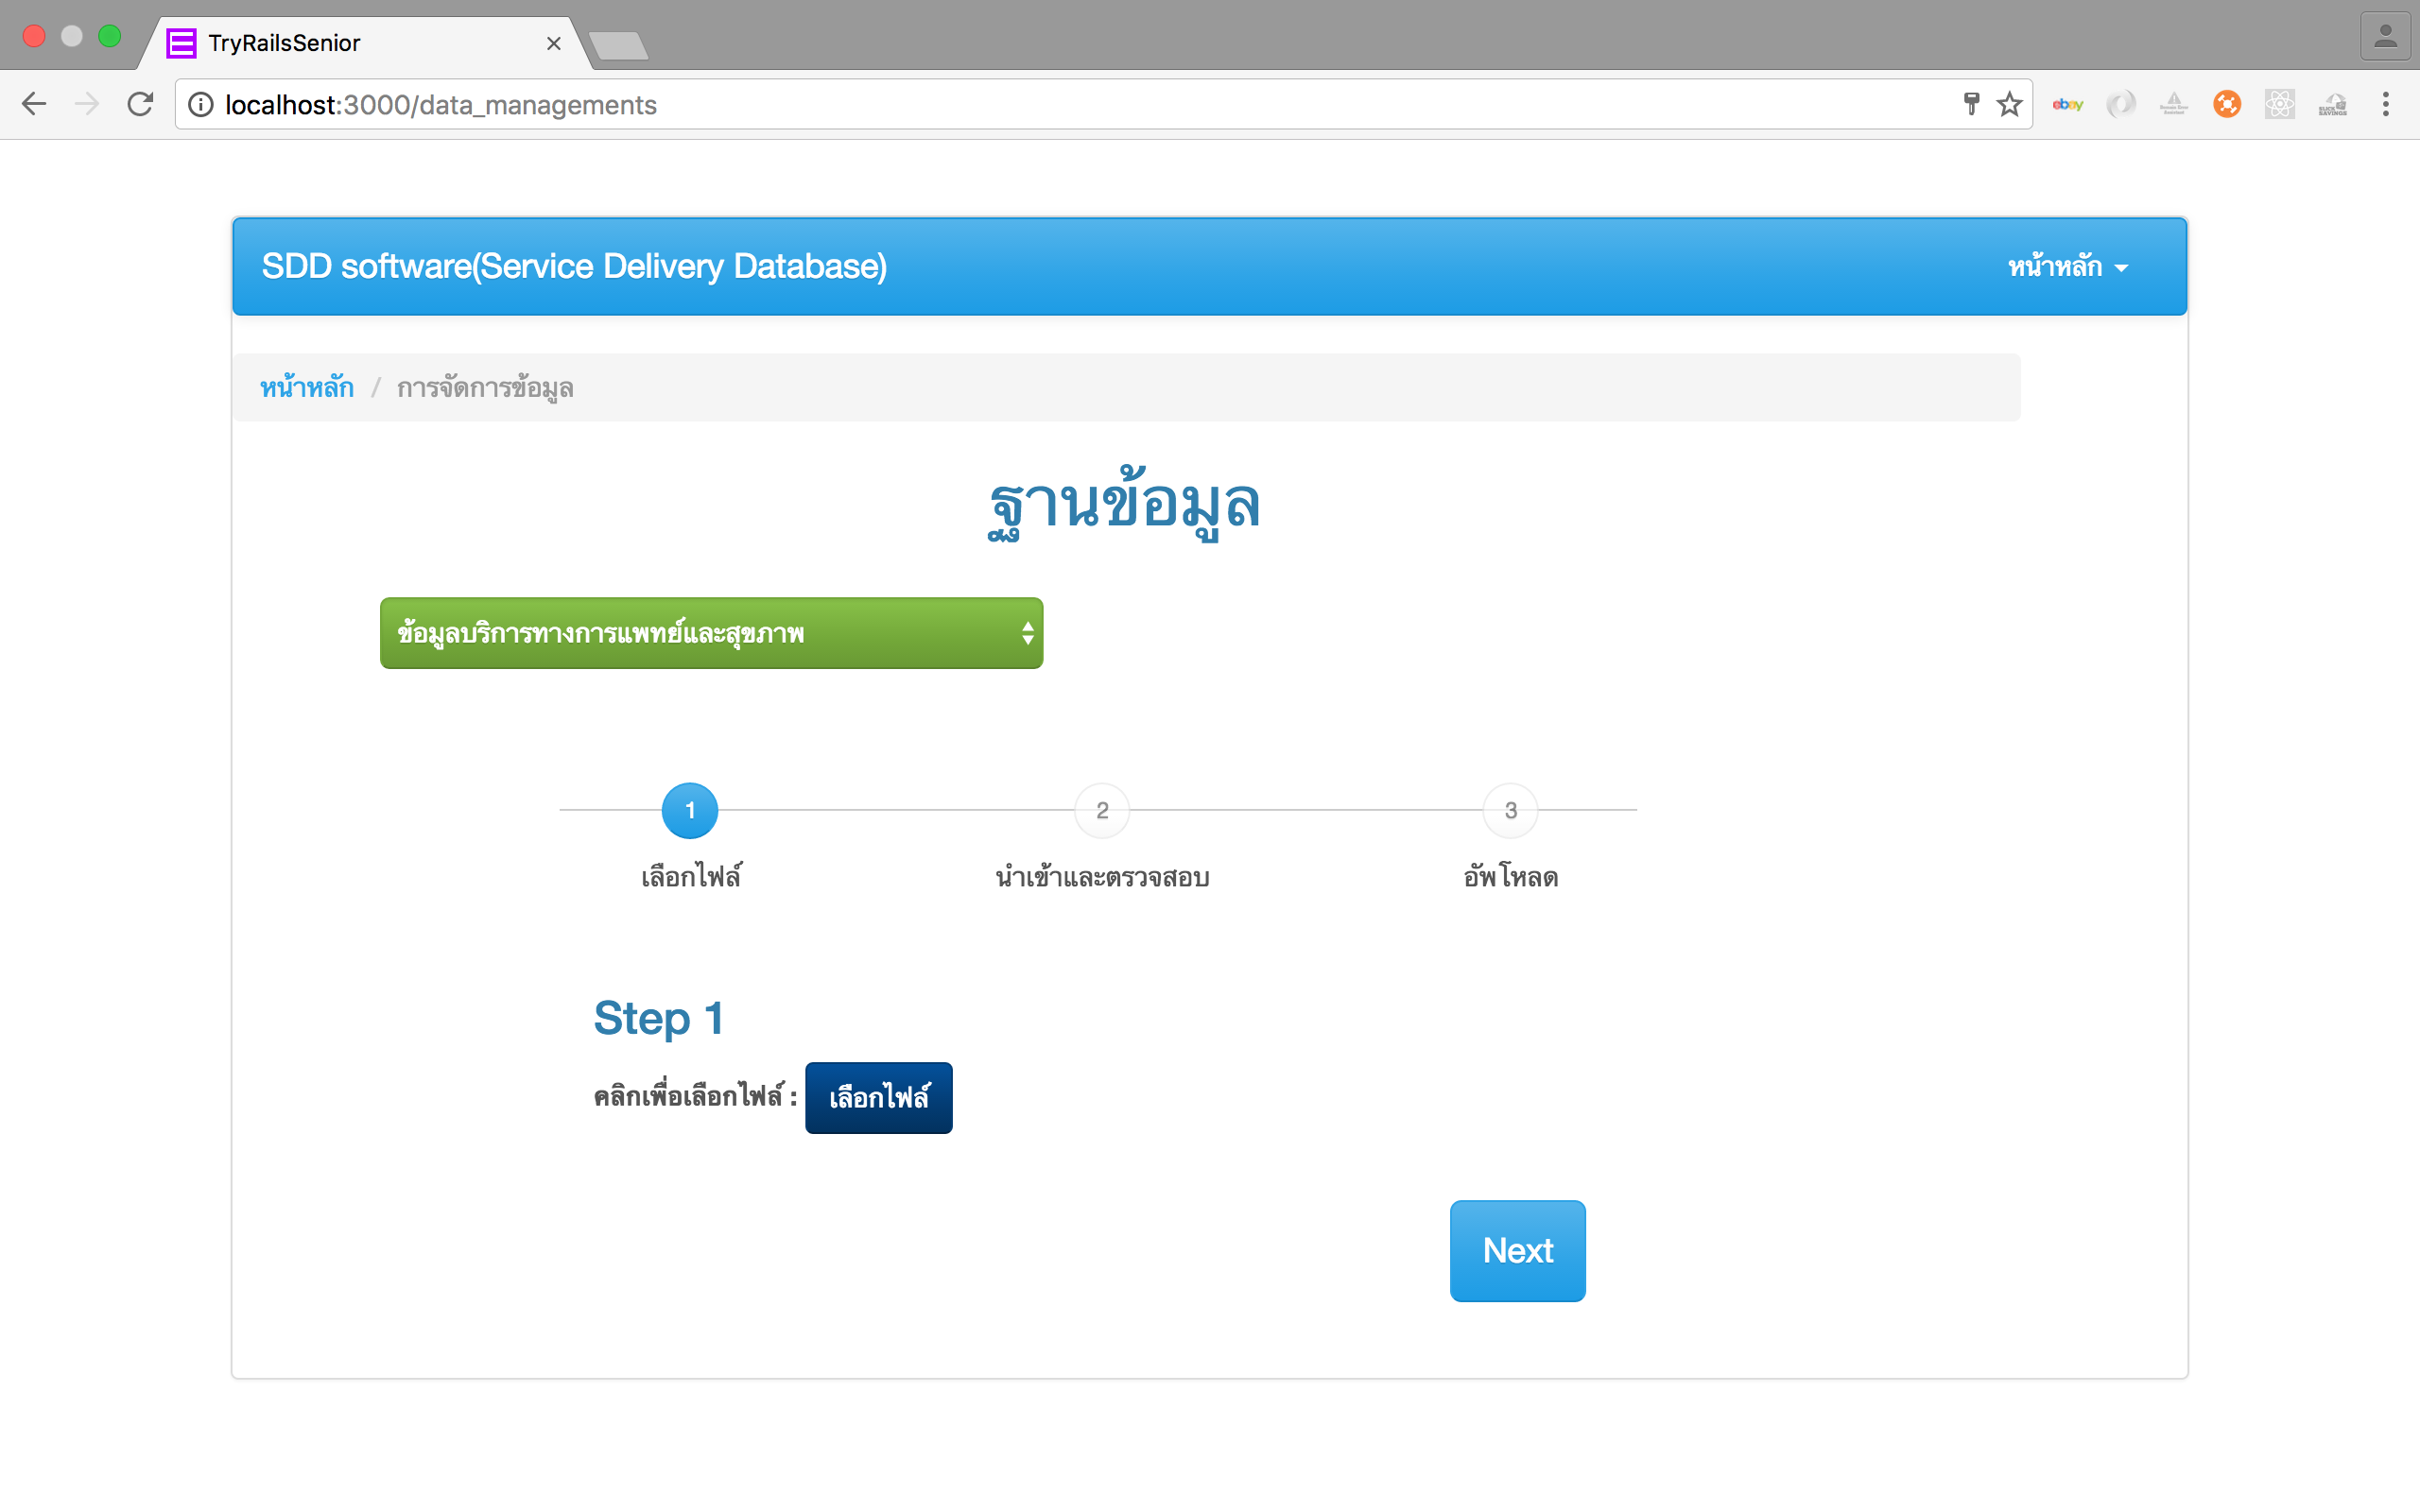
\includegraphics[width=12cm]{images/chapter-01/mockup_rails/upload.png}
                    	\caption{Upload Page Status 1}
                    	\label{upload}
                \end{figure}
            \FloatBarrier
            
           \FloatBarrier
                \begin{figure}[h!]
                    \centering
                        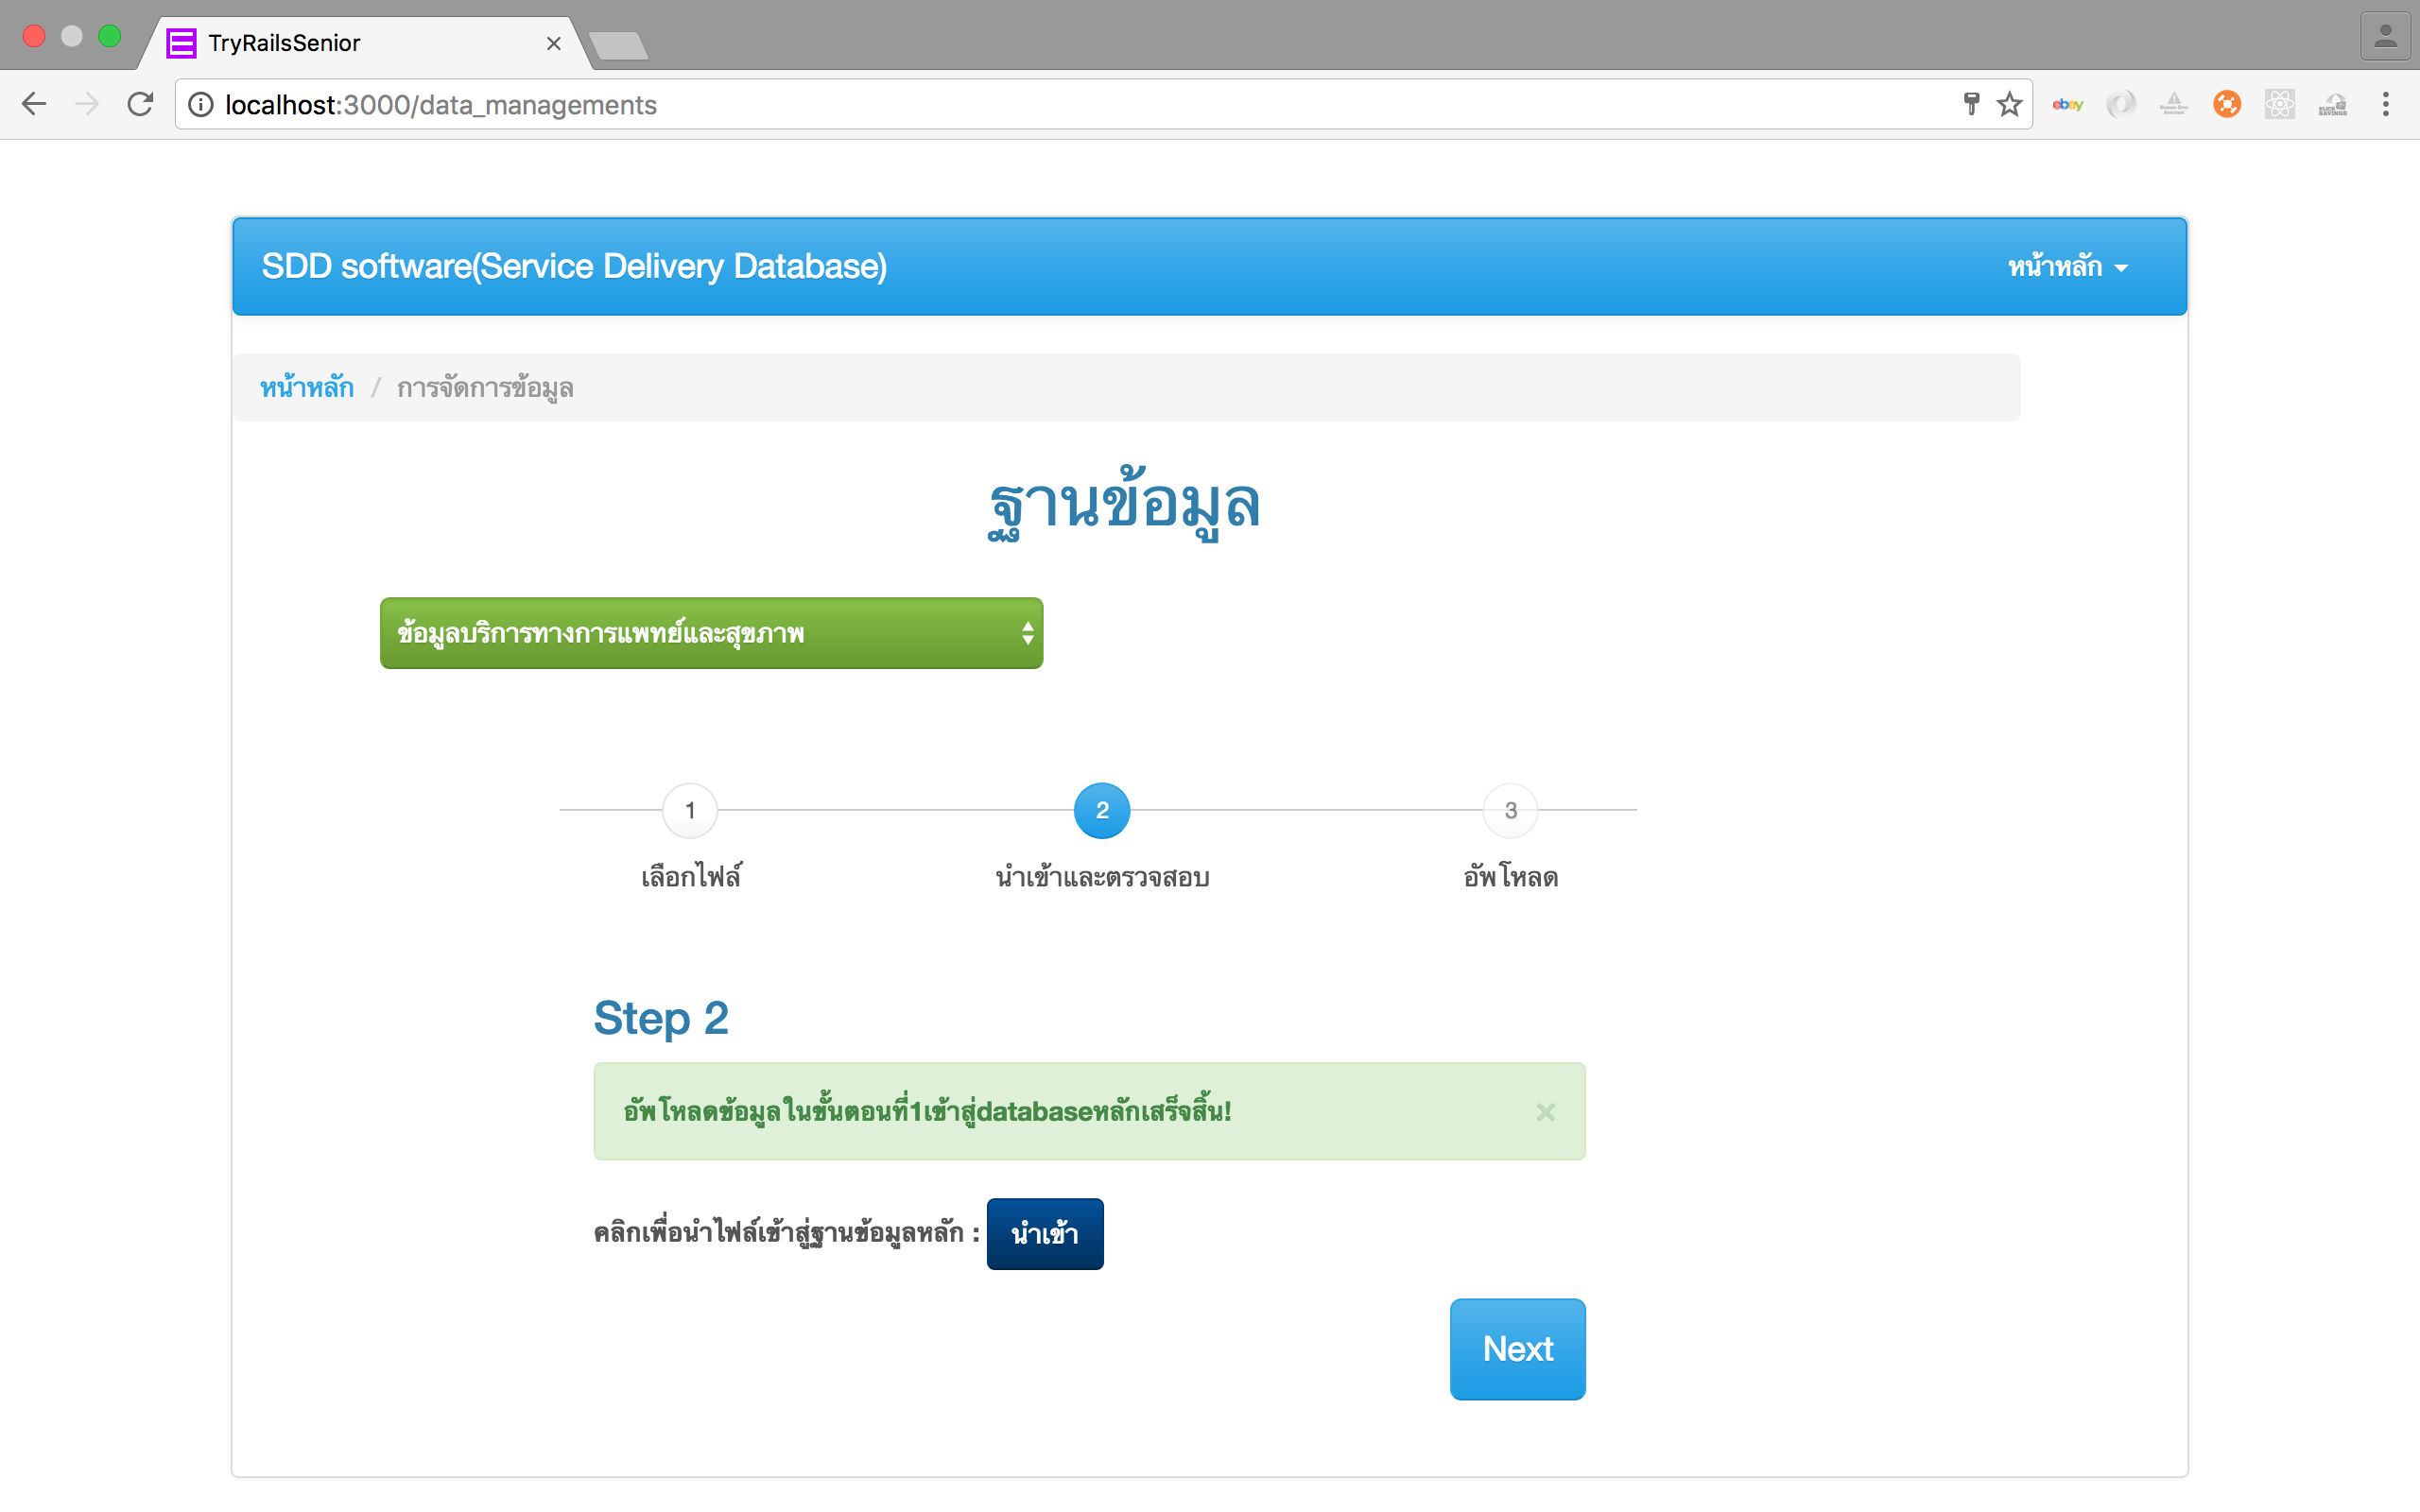
\includegraphics[width=12cm]{images/chapter-01/mockup_rails/upload2.png}
                    	\caption{Upload Page Status 2}
                    	\label{upload2}
                \end{figure}
            \FloatBarrier
            
            \FloatBarrier
                \begin{figure}[h!]
                    \centering
                        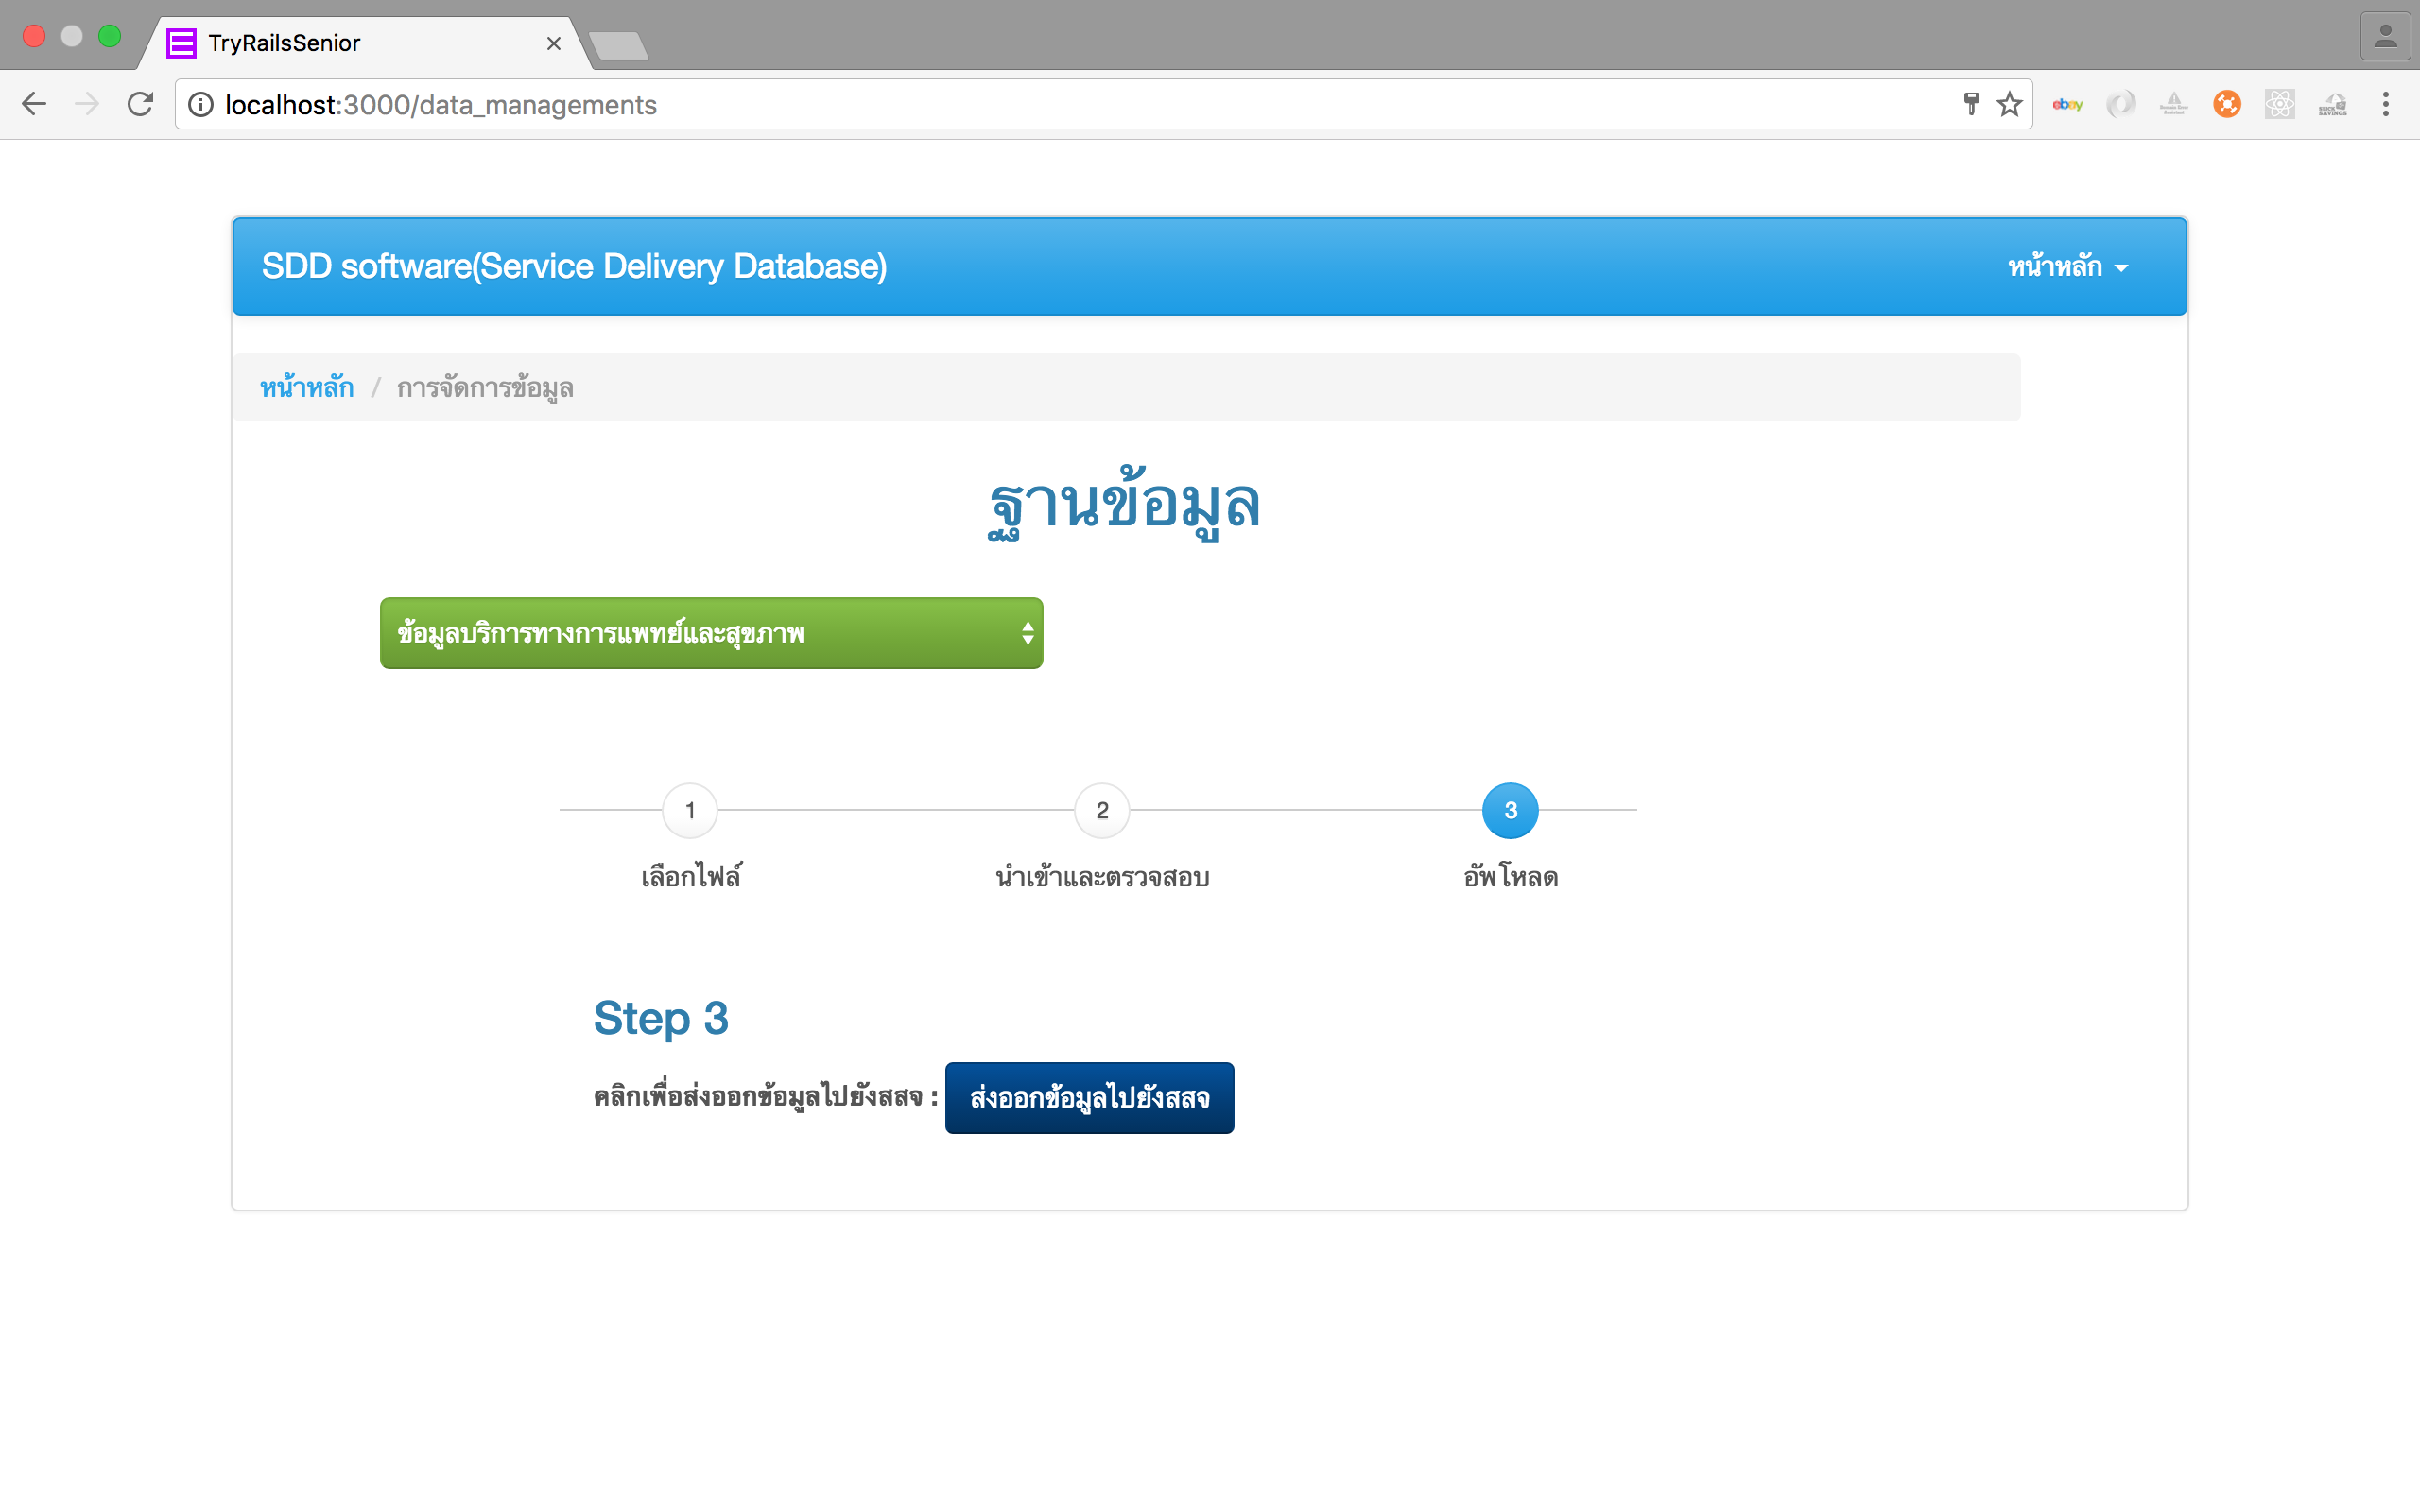
\includegraphics[width=12cm]{images/chapter-01/mockup_rails/upload3.png}
                    	\caption{Upload Page Status 3}
                    	\label{upload3}
                \end{figure}
            \FloatBarrier
            
            \FloatBarrier
                \begin{figure}[h!]
                    \centering
                        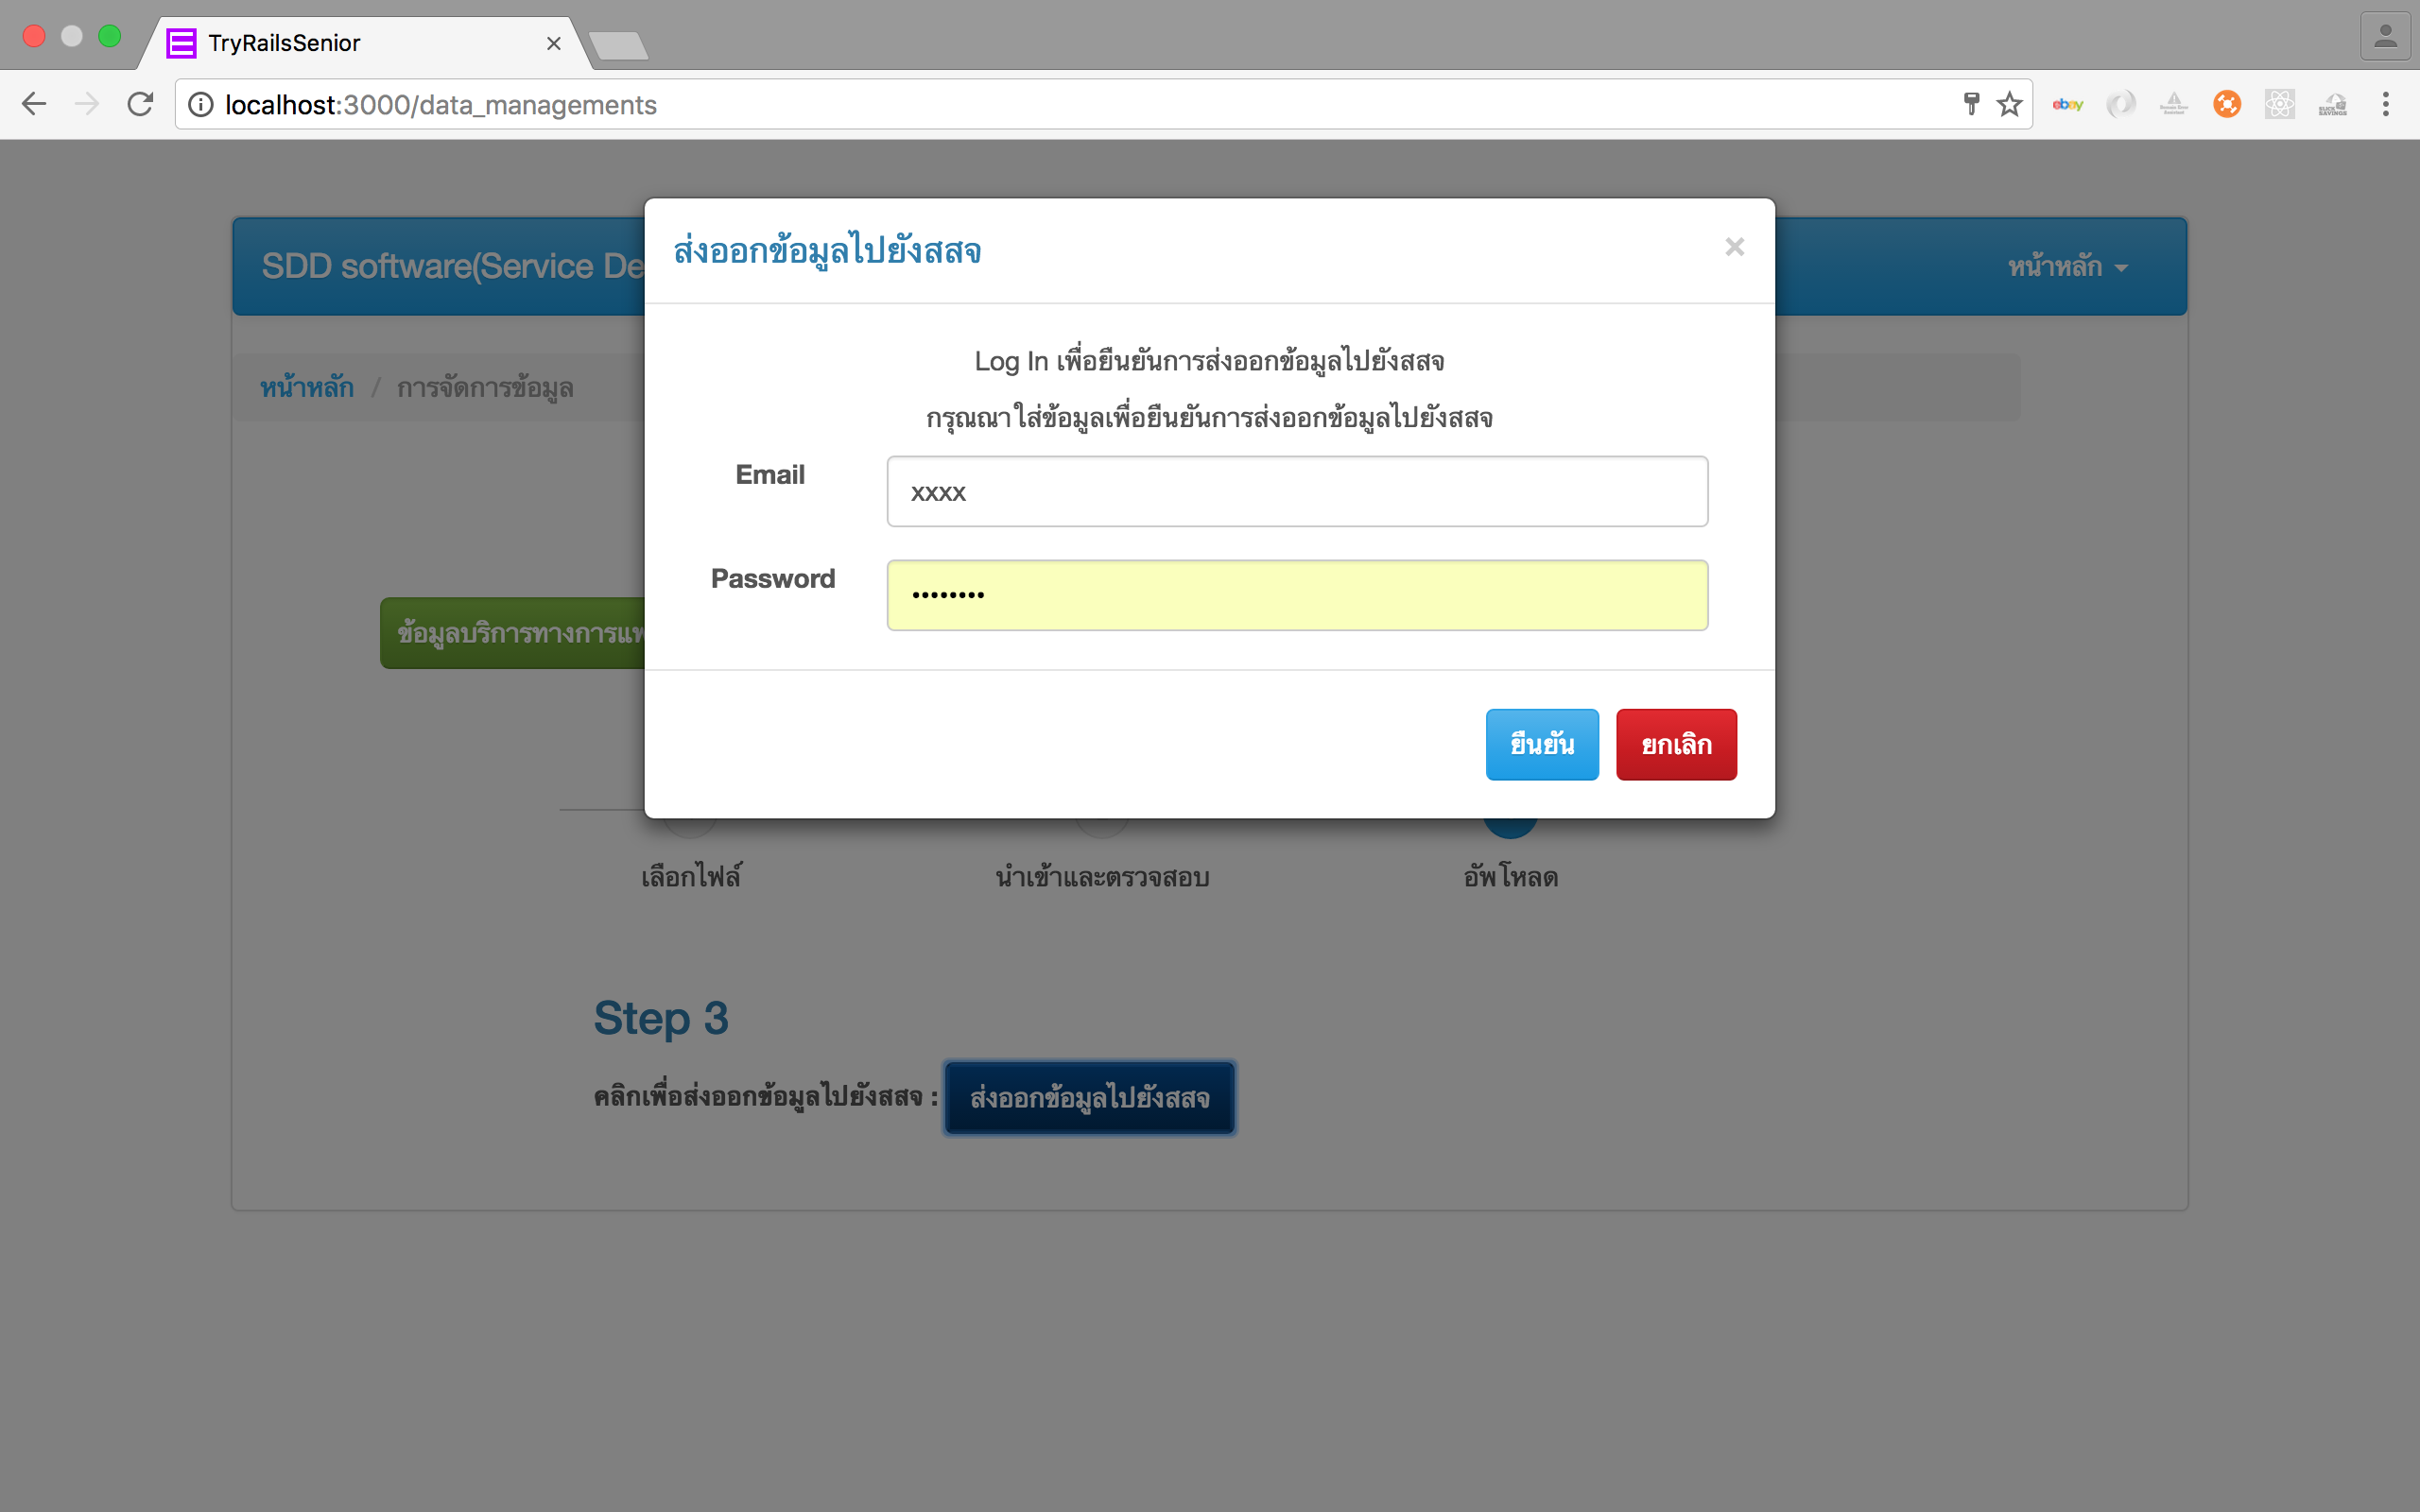
\includegraphics[width=12cm]{images/chapter-01/mockup_rails/upload_confirm.png}
                    	\caption{Upload Confirm Pop Up}
                    	\label{upload_confirm}
                \end{figure}
            \FloatBarrier
            
            \FloatBarrier
                \begin{figure}[h!]
                    \centering
                        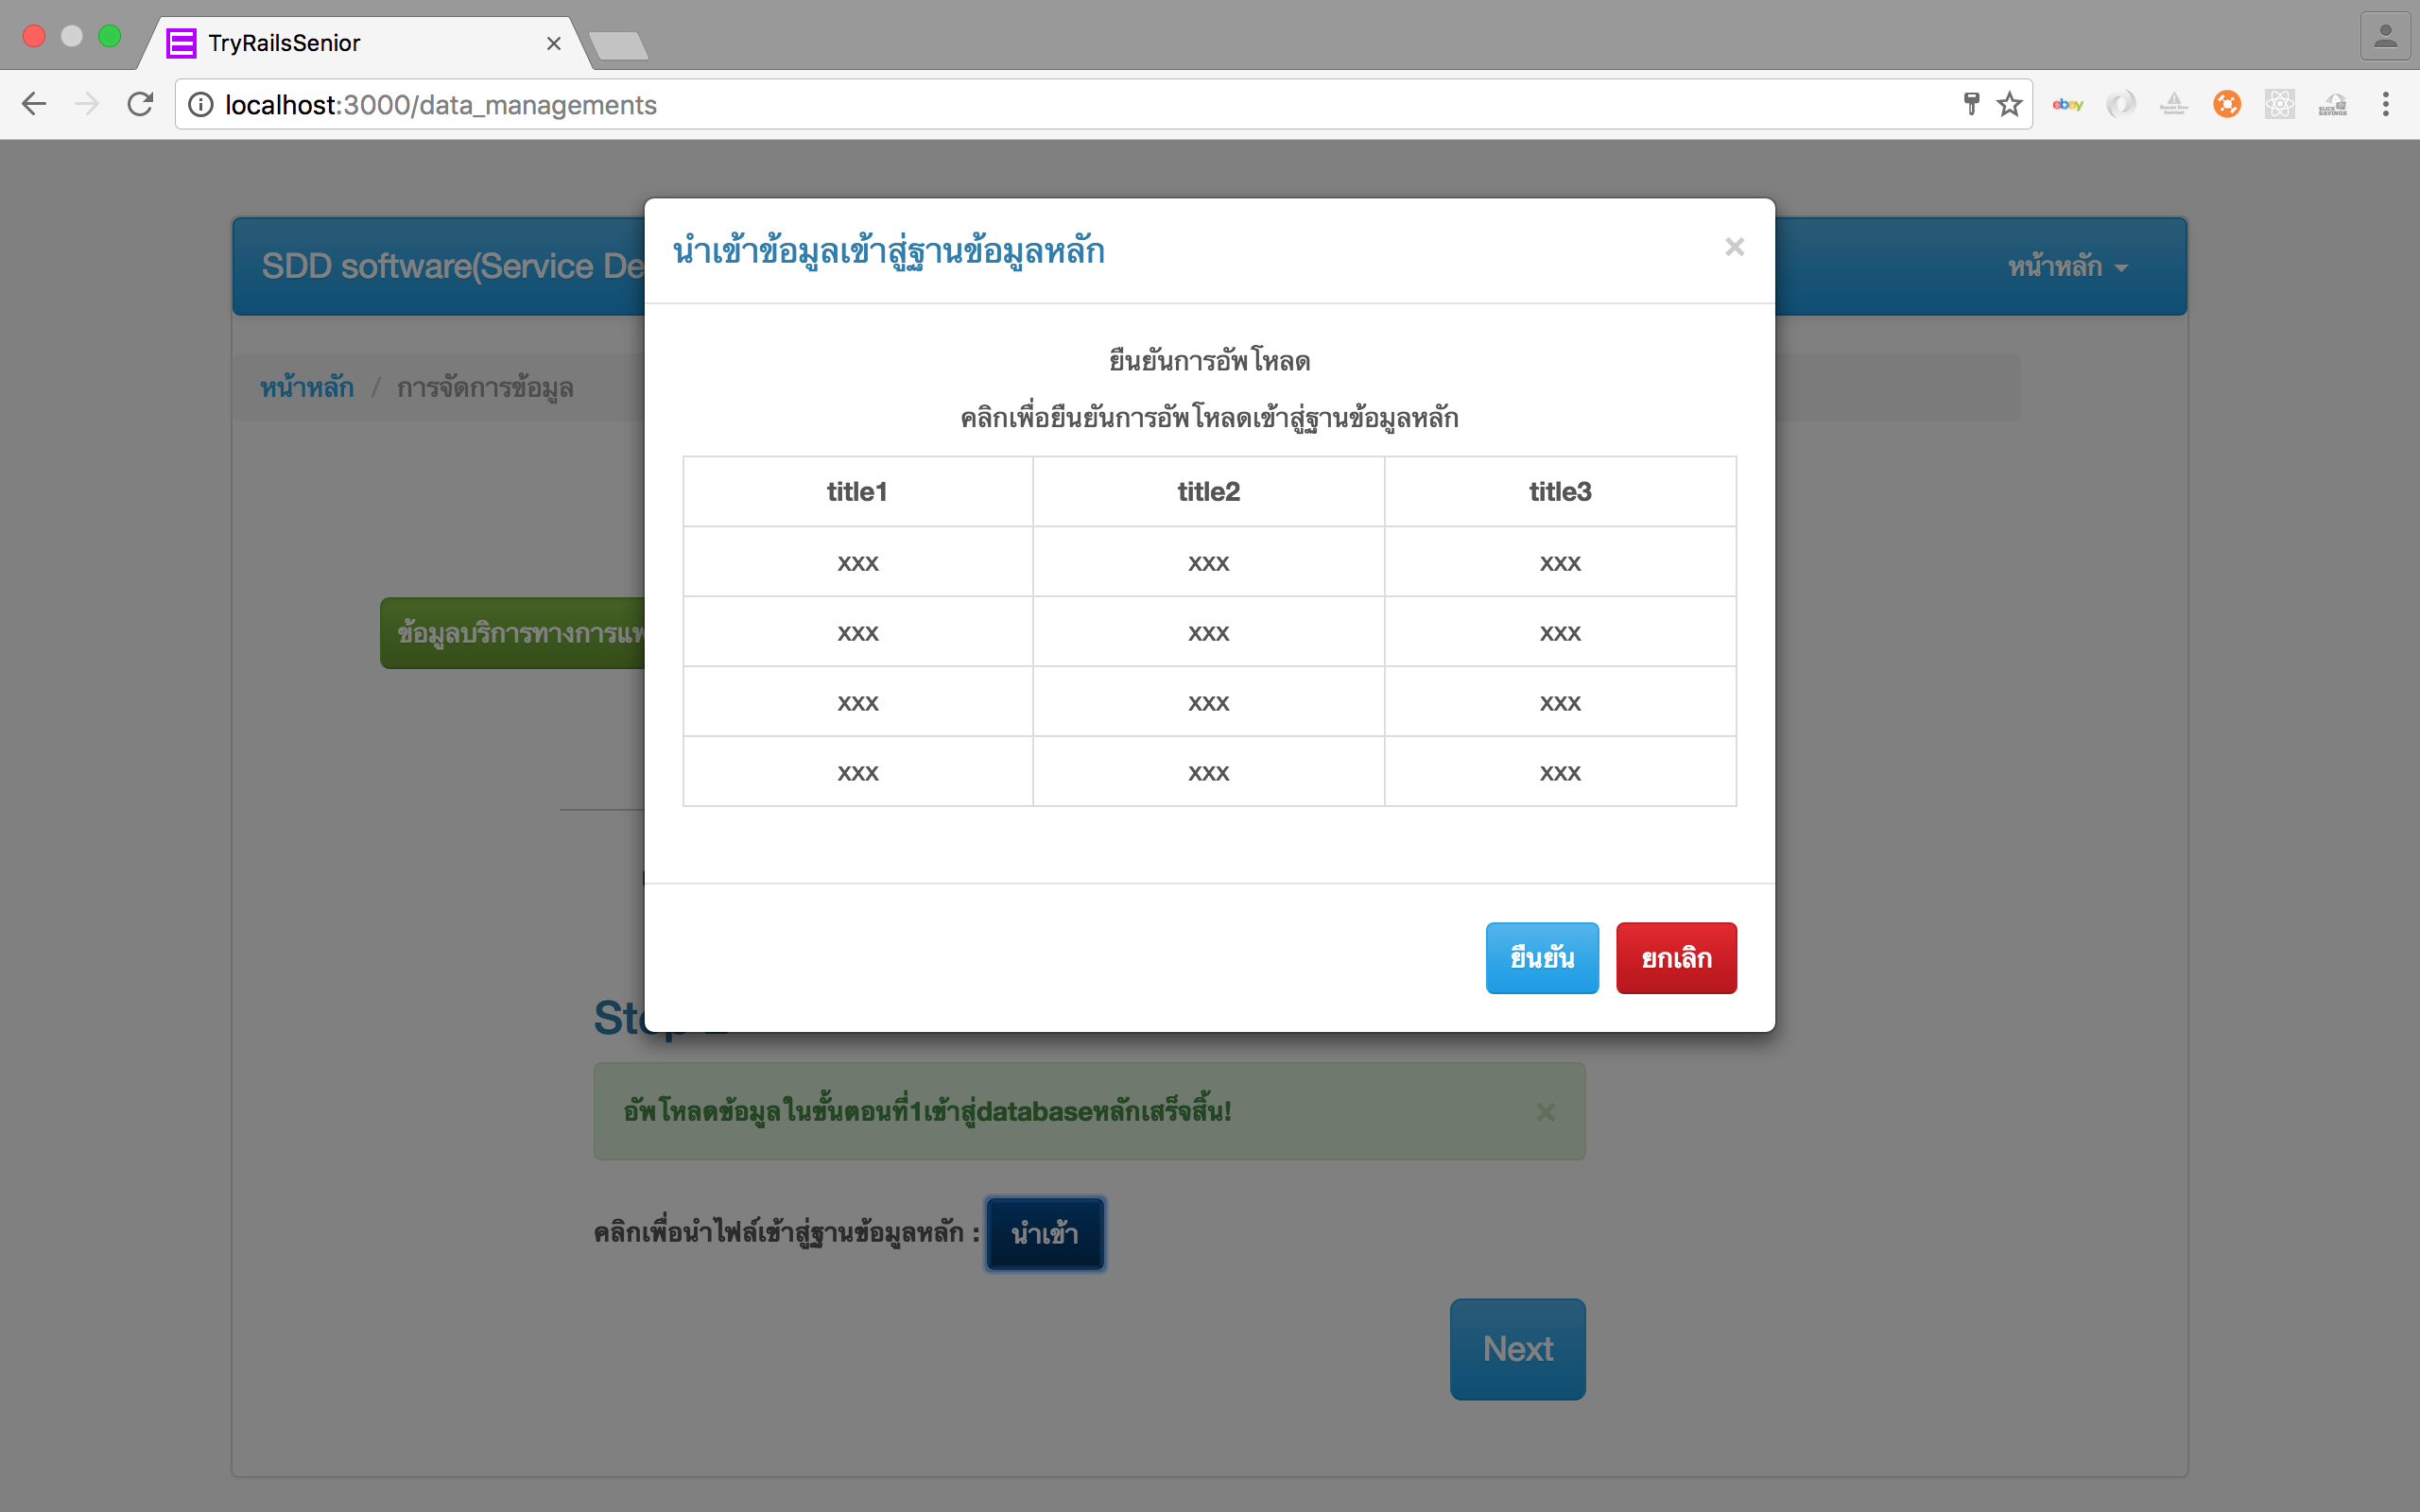
\includegraphics[width=12cm]{images/chapter-01/mockup_rails/upload_verify.png}
                    	\caption{Upload Verify Pop Up}
                    	\label{upload_verify}
                \end{figure}
            \FloatBarrier
            
            \FloatBarrier
                \begin{figure}[h!]
                    \centering
                        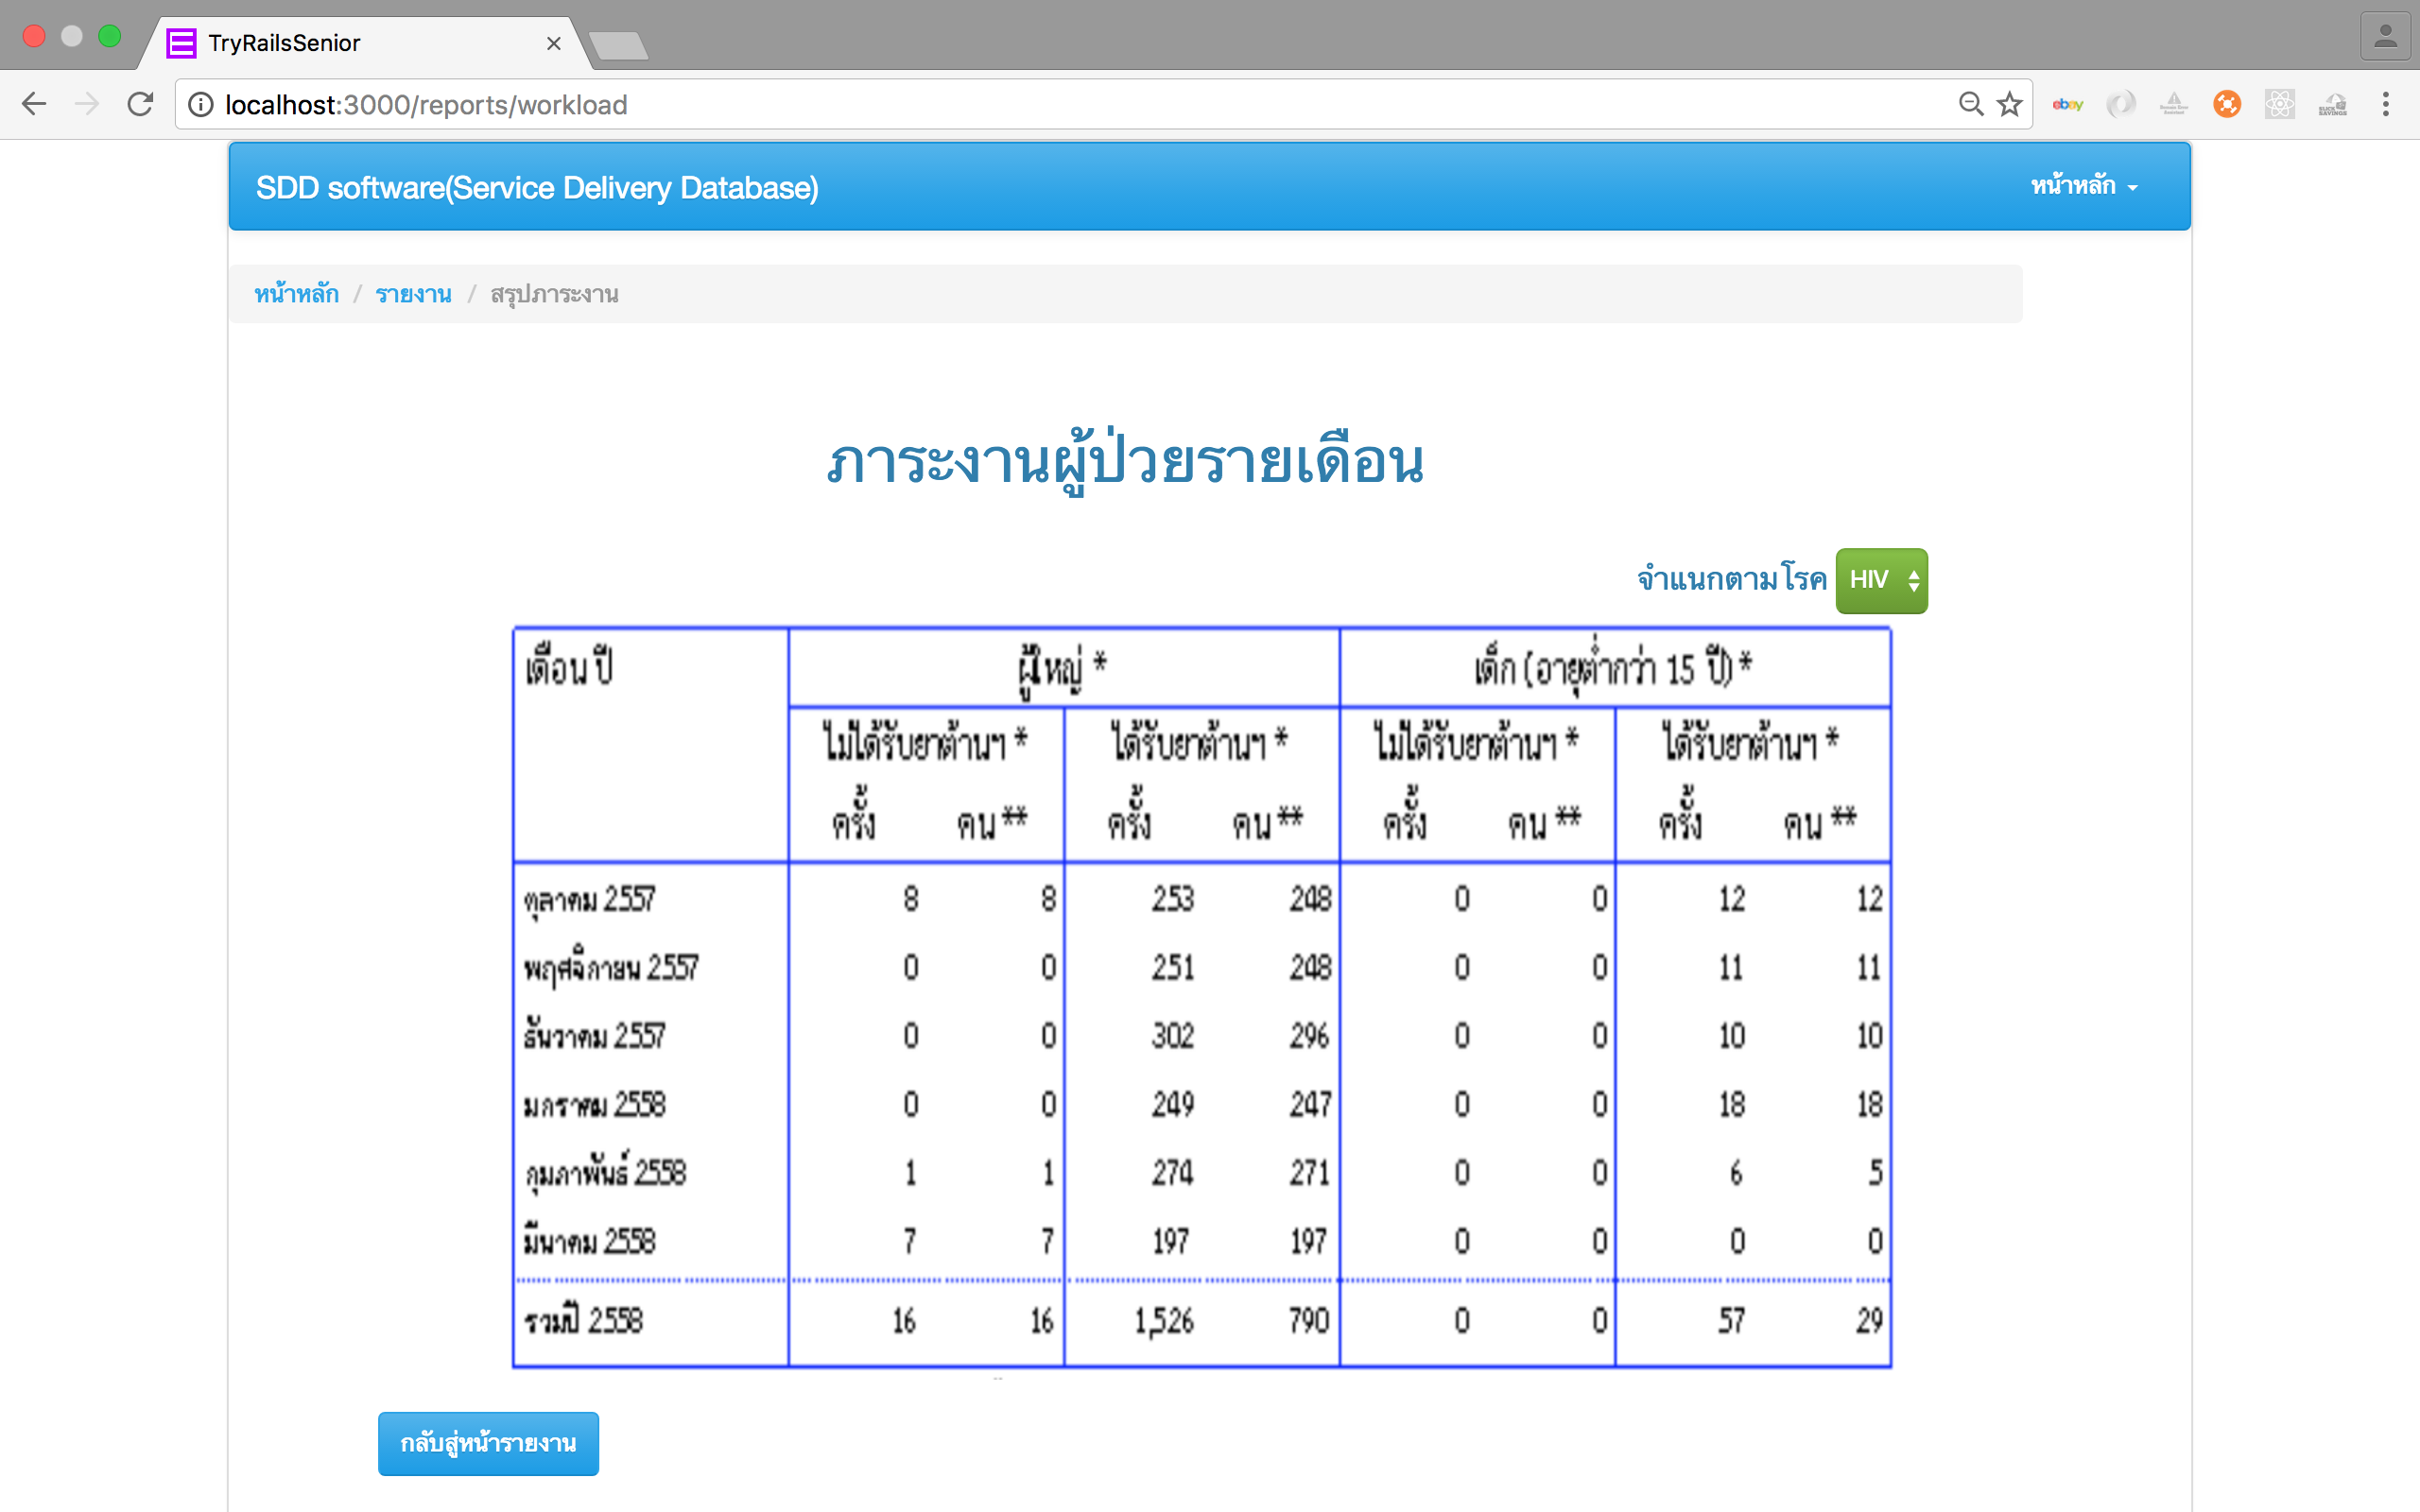
\includegraphics[width=12cm]{images/chapter-01/mockup_rails/report.png}
                    	\caption{Workload Report}
                    	\label{report}
                \end{figure}
            \FloatBarrier
            
            \FloatBarrier
                \begin{figure}[h!]
                    \centering
                        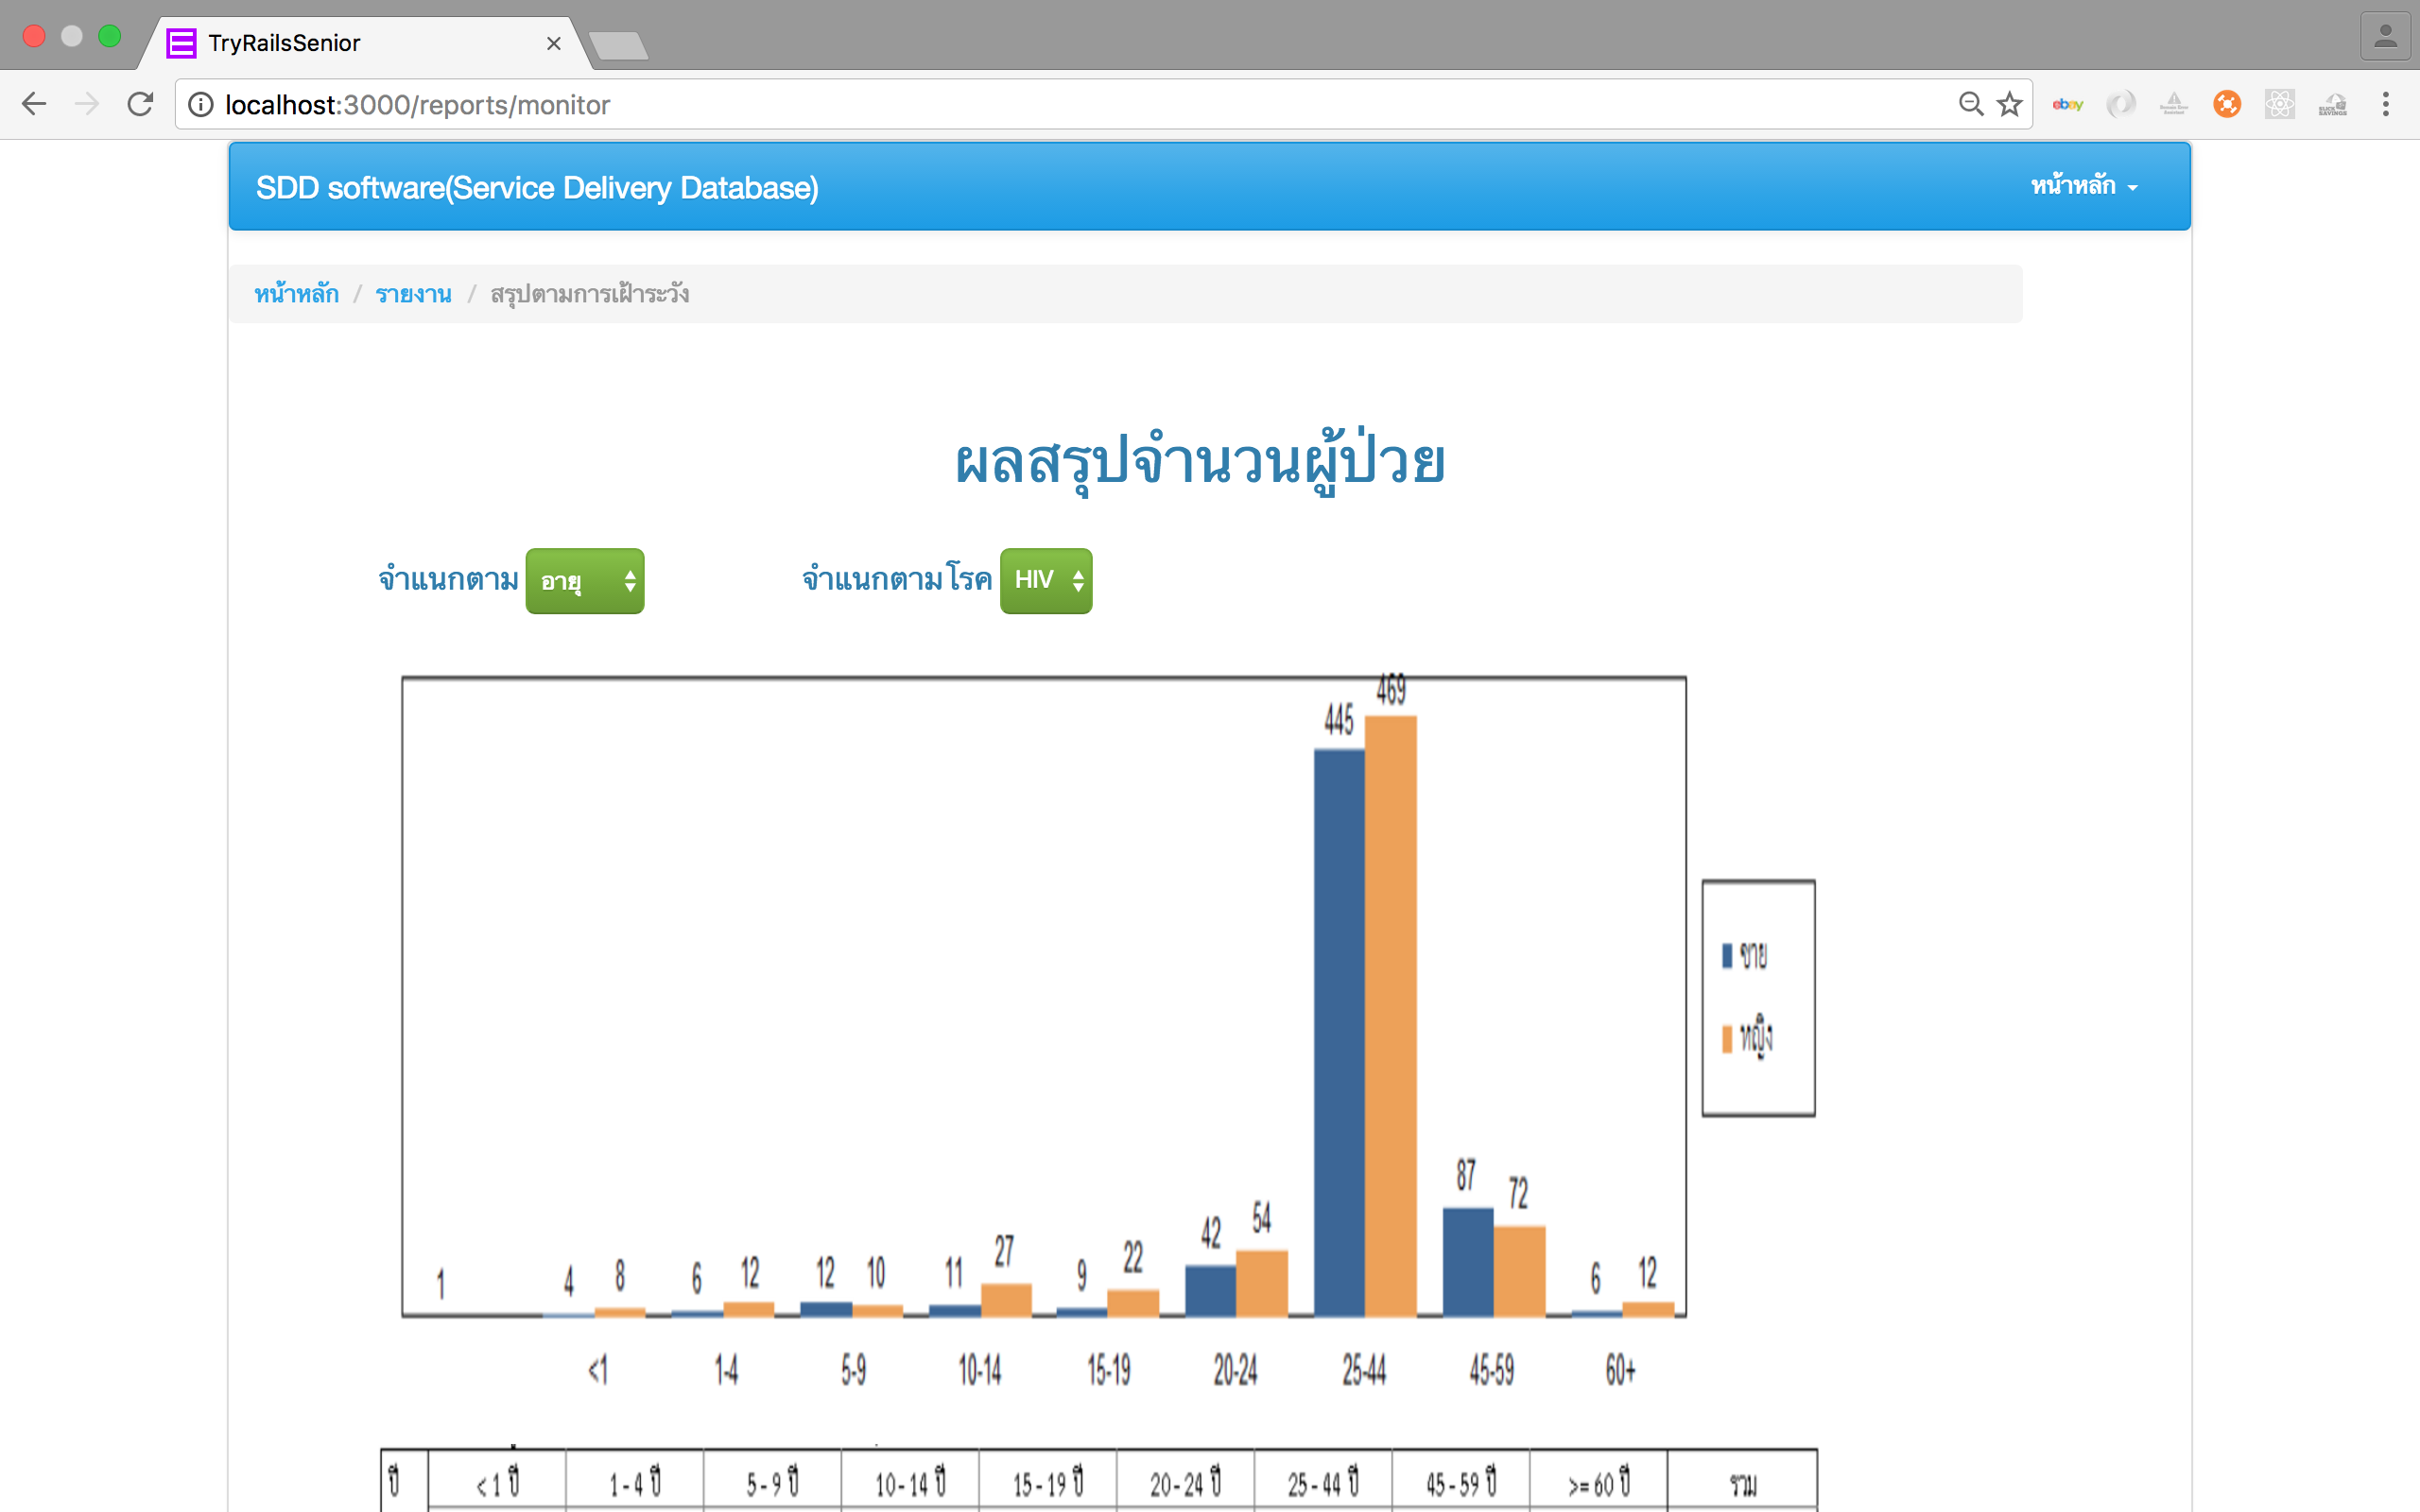
\includegraphics[width=12cm]{images/chapter-01/mockup_rails/report1.png}
                    	\caption{Monitor Report 1}
                    	\label{report1}
                \end{figure}
            \FloatBarrier
            
            \FloatBarrier
                \begin{figure}[h!]
                    \centering
                        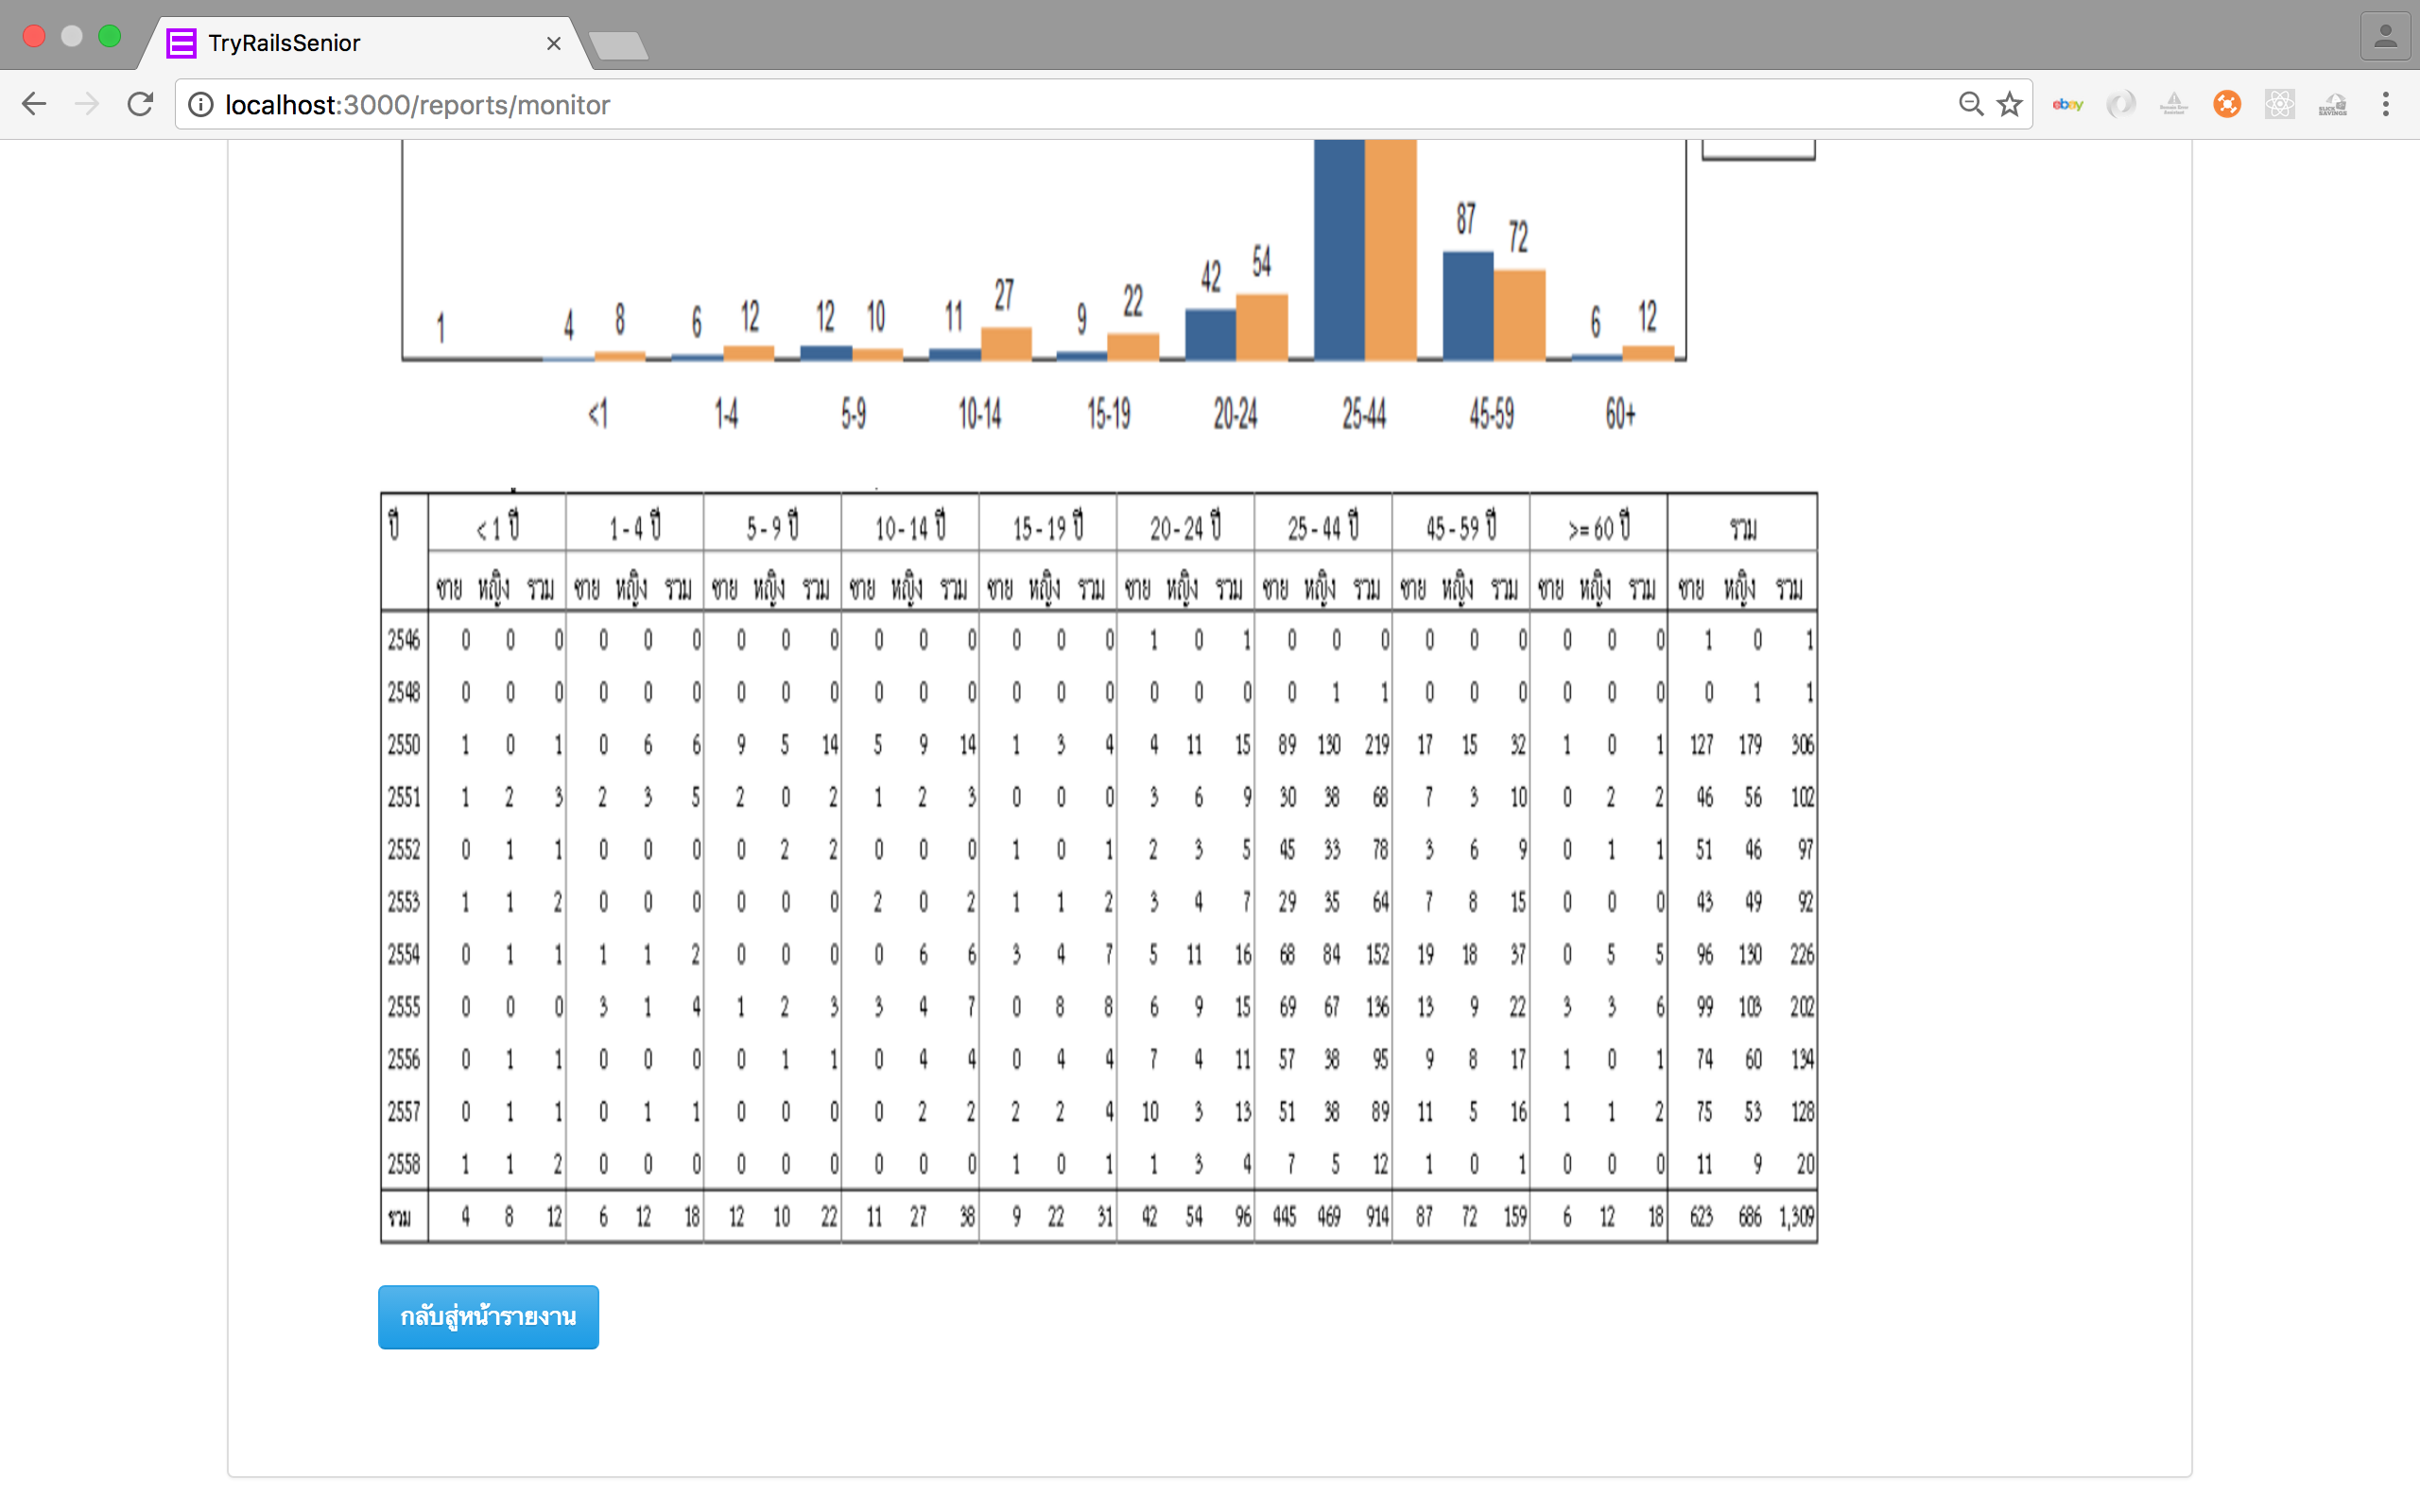
\includegraphics[width=12cm]{images/chapter-01/mockup_rails/report2.png}
                    	\caption{Monitor Report 2}
                    	\label{report2}
                \end{figure}
            \FloatBarrier


	

\section{Technologies}
    The following sections are the technologies and tools that we use for developing Epidemic Intelligent Information System.
    
    \subsection{Docker}
        Docker\cite{docker} is a software for automation deployment of the applications into containers. By using Docker containers, everything that is needed for the application to be able to run is packed into separated containers.
        
        In addition, Docker containers are not virtual machines. It does not need a separated operating system since it is built on top of Linux kernel. However, it depends on the functionality of the kernel and uses resource isolation (CPU, memory, block I/O, network, etc.). Because Docker containers are lightweight, we can run more applications on the server using Docker containers comparing to virtual machines.
        
    \subsection{MongoDB}
        MongoDB\cite{mongodb} is classified as NoSQL database which is an open source database that uses a document oriented data model. Instead of using tables and rows as relational database like SQL, MongoDB consist sets of key-value pairs , and collections are a set of documents and functions.  Like other NoSQL database, MongoDB uses a document storage format or we can call as BSON, which gives binary representation of JSON-like document. In addition, it also support dynamic schema design. In this system, we use MongoDB to store only the User data.
                
    \subsection{Nginx}
        Nginx\cite{nginx} is a web server. It can also be used for reverse proxy server, load balancer, and HTTP cache. In the system that we implemented, we use Nginx as a reverse proxy server for routing between our backend and frontend containers.
        
    \subsection{React}
        React\cite{react} is a javascript library for building interfaces which is maintained by Facebook. It is just a view layer in the application. There are several features in React. First, everything in React is component. The component mainly has state and props. The state is mutable while props is immutable meaning the value of state can be change over time while props can not be changed. This means it is one way data flow which make the behavior of the application predictable. Second, another feature of React is the use of "virtual Document Object Model" or "virtual DOM". The virtual DOM is used for efficient re-rendering of the DOM. This let the programmer to write code as if the entire page is rendered on each change of the data while the React renders only the subcomponent that only changes
        
    \subsection{Scalatra}
        Scalatra\cite{scalatra} is an open source web application framework which is written in scala. It is inspired from Sinatra framework which is implemented using Ruby. It is a microframework which gives developer more freedom because of its minimal.


% Should be on Deploy chapter???
% \section{Failure Handling}
%     Failure handling in this project is convenient since we containerized our application using Docker. There are restart policies\cite{docker_restart_policy} that Docker has provided. The restart policy that we are using in the system is "unless-stopped" which means it will always restart the container no matter the exit status is but it will not restart the container if the container is stopped by the user.
    \chapter{Data Sources}
\section{National Health Service Standard 43 folder}
    National Health Service Standard 43 folder or 43 folder is a collection of more than 43 folder legislate from Ministry of Public Health (MoPH). In 43 folder, there are several information about the patients such as visiting information, diagnosis from both doctor and lab test, type and amount of drug that patient receive and what type of disease that patient have. This 43 folder cover nearly all of the patient information in Thailand including immigrant worker and foreigner, however it is only include patients information from hospital that under Ministry of Public Health (MoPH) exclude Bangkok. This is because hospital in Bangkok is under the management of Bangkok Administration.
    
\section{Data Schema}
    In our system, we do not need all 43 folders to process the data. We only need the following folders.
    
    % Thai officer position in English
    % http://wangkapee.uttaradit.police.go.th/InPos.html
    % https://web.facebook.com/Ed1BO/posts/494806177306805?_rdr
    
    \subsection{PERSON}
        In this folder, it stores the data of patient who does not live in hospital's region or patient who lives in hospital's region but his/her household registration is not in hospital's region. It is consist of hospcode(hospital code), CID (Citicen ID), PID (Patient ID), name, birth date and etc. For complete detail of PERSON folder you can look at \ref{person_folder}.
    
    \subsection{ADDRESS}
        In this folder, it stores the address of a patient who lives outside responsible district or patient who live inside responsible district but his/her household registration is outside the district.For complete detail of ADDRESS folder you can look at \ref{address_folder}.
        
        % % http://www.dailyenglish.in.th/english-address/
\begin{enumerate}
  \item HOSPCODE: Hospital code that is defined by the Bureau of Policy and Strategy (under Ministry of Public Health). 
  \item PID: Person identification number who registers in the hospital. This is used for identifying the person in other folders (the range of digits can be between 1 to 15 and generated by program).
  \item ADDRESSTYPE: Type of address. 1 = Address in household registration, 2 = Address that is reachable by contact.
  \item HOUSE\_ID: House identification number that is assigned by Department of Provincial Administration (under Ministry of Interior).
  \item HOUSE\_TYPE: The type of residence. 1 = Detached House or Semi Detached House, 2 = Townhouse, 3 = Condominium, 4 = Apartment or Dormitory, 5 = Labor Home-stay, 8 = etc, 9 = unknown.
  \item ROOMNO: The room number if HOUSE\_TYPE is an apartment or dormitory.
  \item CONDO: The name of building, condominium, or dormitory.
  \item HOUSENO: Street number
  \item SOISUB: Sub lane
  \item SOIMAIN: Lane
  \item ROAD: The road's name
  \item VILLANAME: The village's name
  \item VILLAGE: The village number. Use 99 if unknown.
  \item TAMBON: Sub district code that is defined by Department of Provincial (under Ministry of Interior). Use 99 if unknown.
  \item AMPUR: District code that is defined by Department of Provincial (under Ministry of Interior). Use 99 if unknown.
  \item CHANGWAT: Province code that is defined by Department of Provincial (under Ministry of Interior). Use 99 if unknown.
  \item TELEPHONE: Telephone number
  \item MOBILE: Mobile phone number
  \item D\_UPDATE: The date in which this folder has been modified. The format is YYYYMMDDHHMMSS and the year format is CE.
\end{enumerate}
        
    \subsection{DEATH}
        This folder stores the history of death of citizens who lived in the responsible district and patient. It consists of death date, disease code and etc.For complete detail of DEATH folder you can look at \ref{death_folder}.
        % \begin{enumerate}
  \item HOSPCODE: Hospital code that is defined by the Bureau of Policy and Strategy (under Ministry of Public Health). 
  \item PID: Person identification number who registers in the hospital. This is used for identifying the person in other folders (the range of digits can be between 1 to 15 and generated by program).
  \item HOSPDEATH: Hospital code in a case that patient died in the hospital. If they can not determine which hospital, mark it as 00000.
  \item AN: Inpatient number in which the patient died in the hospital
  \item SEQ: The order of the service that be provided by the program. the number is unique, and sort by order of SEQ in each service (visit).
  \item DDEATH: Date that patient died. The format is YYYYMMDD and the year format is CE.
  \item CDEATH\_A: Disease code A according to Certificate of Death. 
  \item CDEATH\_B: Disease code B according to Certificate of Death.
  \item CDEATH\_C: Disease code C according to Certificate of Death.
  \item CDEATH\_D: Disease code D according to Certificate of Death.
  \item ODISEASE: Other disease code or other factor of death according to Certificate of Death.
  \item CDEATH: Cause of death according to the Certificate of Death.
  \item PREGDEATH: 1 = Death in pregnancy, 2 = Maternal Death
  \item PDEATH: The place where patient died. 1 = In hospital, 2 = Outside hospital.
  \item PROVIDER: Doctor of patient number that is generated by the program. It must be unique within the same hospital.
  \item D\_UPDATE: The date in which this folder has been modified. The format is YYYYMMDDHHMMSS and the year format is CE.
\end{enumerate}
        
    \subsection{SERVICE}
        In this folder, it contains the data about the history of the service that be provided to the patient who come to receive and also provide the service outside the hospital area.For complete detail of SERVICE folder you can look at \ref{service_folder}.
        % \begin{enumerate}
  \item HOSPCODE: Hospital code that is defined by the Bureau of Policy and Strategy (under Ministry of Public Health). 
  \item PID: Person identification number who registers in the hospital. This is used for identifying the person in other folders (the range of digits can be between 1 to 15 and generated by program).
  \item HN: Outpatient number that receive when the patient come to receive the service (the range of digits can be between 1 to 15)
  \item SEQ: The order of the service that be provided by the program. the number is unique, and sort by order of SEQ in each service (visit).
  \item DATE\_SERV: The date receiving the service. Defining format as year (in CE format), month and date  by order(YYYYMMDD). NOTE that in case have to record previous data, have to change the date to the date that receive the service.
  \item TIME\_SERV: Time hospital provide a service and defining format as  hour, minute, and second as (HHMMSS)  
  \item LOCATION: The area of the patient. There are two type of it which are (1) means area of responsibility and (2) means area of irresponsibility
  \item INTIME: The time that patient come and receive the service. There are two type of it which are (1) means in office hours and (2) means out of the office hours.
  \item INSTYPE: The right to medical care code that the patient use each visit.
%   ประเภทสิทธิการรักษา
%   รหัสสิทธิมาตรฐาน ที่ใชในการมารับบริการ
  \item INSID: The id number of the card of the right to medical care according to the type of the right to medical care.
%   หมายเลขของบัตร ตามประเภทสิทธิการรักษา
  \item MAIN: The standard code that come from Bureau of Policy and Strategy in order to describe the main service place.
  \item TYPEIN: It is a types of service that patient come to receive the service. There are four main types which are (1) means the patient come to receive the service by themselves, (2) means the patient come to receive the service according to the appointment, (3) means the patient that be transferred from one to other hospital, and (4) means the patient that be transferred from EMS.
  \item REFERINHOSP: The code of the hospital that send the patient to here. 
  \item CAUSEIN: The reason that transfer the patient to receive the service here. There are five main types which are (1) means to diagnose and treat, (2) means to diagnose, (3) means to treat and recover, (4) means to receive the service that close to their home, and (5) means to receive the service according to the patient's need.
  \item CHIEFCOMP: The important symptoms that patient has to come to use the service.
  \item SERVPLACE: The place that receive the service. There are 2 types which are (1) means in the service place and (2) means outside the service place
  \item BTEMP: The body temperature that measure when the patient come in. It should be in Celsius with two digits and one decimal place.
  \item SBP: Systolic pressure that first given. It should be three or less than three digits. Note that if cannot measure, not need to record
  \item DBP: Diastolic pressure that first given. It should be three or less than three digits. Note that if cannot measure, not need to record
  \item PR: Heart rate per minute. It should be three or less than three digits.
  \item RP: Breath rate per minute. It should be three or less than three digits.
  \item TYPEOUT: The status of patient after they are done receiving the service. There are nine main types which are (1) means receive drug and can go back home, (2) means receiving as Inpatient, (3) means the patient is sent to other hospital, (4) mean dead, (5) means dead before receiving the service at hospital, (6) means dead during the transfer process to other hospital, (7) means decline to treat. (8) means escape. (9) mean receive the service without diagnosis result.
  \item REFEROUTHOSP: The hospital code that transfer the patient to have a treatment.
  \item CAUSEOUT: The reason to transfer the patient to receive the service. There are five main types which are (1) means to diagnose and treat, (2) means to diagnose, (3) means to treat and recover, (4) means to receive the service that close to their home, and (5) means to receive the service according to the patient's need.
  \item COST: Total cost of treatment including drug, medical supplies, treatment. It should be eight digits and two decimal place. If it is no price, put 0.00.
  \item PRICE:Total price of treatment including drug, medical supplies, treatment. It should be eight digits and two decimal place. If it is no price, put 0.00.
  \item PAYPRICE: Total price that patient have to pay since it is the expenses that cannot be issued to the government. . It should be eight digits and two decimal place. If it is no price, put 0.00.
  \item ACTUALPAY: Total price that the patient have to pay. It should be eight digits and two decimal place. If it is no price, put 0.00.
  \item D\_UPDATE: The date in which this folder has been modified. The format is YYYYMMDDHHMMSS and the year format is CE.
  
  
\end{enumerate}
        
    \subsection{DIAGNOSIS\_OPD}
        In this folder, it contains the diagnosis of the Out-patient and patient who come to receive the service. For complete detail of DIAGNOSIS\_OPD folder you can look at \ref{diagnosis_opd_folder}.
        % \begin{enumerate}
  \item HOSPCODE: Hospital code that is defined by the Bureau of Policy and Strategy (under Ministry of Public Health). 
  \item PID: Person identification number who registers in the hospital. This is used for identifying the person in other folders (the range of digits can be between 1 to 15 and generated by program).
  \item SEQ: The order of the service that be provided by the program. the number is unique, and sort by order of SEQ in each service (visit).
  \item DATE\_SERV: The date receiving the service. Defining format as year(Anno Domini(AD)), month and date  by order(YYYYMMDD). NOTE that in case have to record previous data, have to change the date to the date that receive the service.
  \item DIAGTYPE: Type of diagnosis. 1 = Principle DX, 2 = Co-Morbidity, 3 = Complication, 4 = other, 5 = External Cause, 6 = Additional Code, 7 = Morphology Code. In case of out-patient, use only 1, 4, 5 or 7.
  \item DIAGCODE: Disease code in ICD-10-TM
  \item CLINIC: Ward code that is defined by the Bureau of Policy and Strategy (under Ministry of Public Health).
  \item PROVIDER: Doctor of patient number that is generated by the program. It must be unique within the same hospital.
  \item D\_UPDATE: The date in which this folder has been modified. The format is YYYYMMDDHHMMSS and the year format is CE.
\end{enumerate}
        
    \subsection{DRUG\_OPD}
        In this folder, it contains the data that providing drug for Out-patient and patient who come to receive the service. For complete detail of DRUG\_OPD folder you can look at \ref{drug_opd_folder}.
        % \begin{enumerate}
  \item HOSPCODE: Hospital code that is defined by the Bureau of Policy and Strategy (under Ministry of Public Health). 
  \item PID: Person identification number who registers in the hospital. This is used for identifying the person in other folders (the range of digits can be between 1 to 15 and generated by program).
  \item SEQ: The order of the service that be provided by the program. the number is unique, and sort by order of SEQ in each service (visit). 
  \item DATE\_SERV: The date that receive the service Defining format as year(format CE), month and date by order (YYYYMMDD). NOTE that in case have to record previous data, have to change the date to the date that receive the service.
  \item CLINIC: Service department code according to Bureau of Policy and Strategy
  \item DIDSTD: The standard medicine code that is set in 24 digits and the medicine code of hospital in case that they do not have The standard medicine code.
  \item DNAME: Name of the drug
  \item AMOUNT: The amount of medicine that be provided and it has to be in 12 digit(no more than 12 digits)
  \item UNIT: Unit of medicine. It is the standard code that come from Bureau of Policy and Strategy  
  \item UNIT\_PACKING: Packing size per unit that is counting in Field UNIT  
  \item DRUGPRICE: The price of medicine that sell to the patient
  \item DRUGCOST: The buying price or the price of medicine that be received from hospital  
  \item PROVIDER: Service person number that generated from the program and the number is unique in each hospital.
  \item D\_UPDATE: The date in which this folder has been modified. The format is YYYYMMDDHHMMSS and the year format is CE.
\end{enumerate}











        
    \subsection{LABFU}
        In this folder, it stores the  lab result that come from the lab of patient who have diseases. For complete detail of LABFU folder you can look at \ref{labfu_folder}.
        % \begin{enumerate}
  \item HOSPCODE: Hospital code that is defined by the Bureau of Policy and Strategy (under Ministry of Public Health). 
  \item PID: Person identification number who registers in the hospital. This is used for identifying the person in other folders (the range of digits can be between 1 to 15 and generated by program).
  \item SEQ: The order of the service that be provided by the program. the number is unique, and sort by order of SEQ in each service (visit). 
  \item DATE\_SERV: The date receiving the service. Defining format as year(format CE), month and date by order (YYYYMMDD). NOTE that in case have to record previous data, have to change the date to the date that receive the service.
%   Do we need to include ICD-10-TM??
  \item LABTEST: ICD-10-TM Laboratory Test Code
  \item LABRESULT: Results of laboratory tests (2-digit decimal point)
  \item D\_UPDATE:  The date in which this folder has been modified. The format is YYYYMMDDHHMMSS and the year format is CE.
\end{enumerate}


    \subsection{ADMISSION}
        In this folder, it stores the history record of patient's admission of the hospital. For complete detail of ADMISSION folder you can look at \ref{admission_folder}.
        % \begin{enumerate}
  \item HOSPCODE: Hospital code that is defined by the Bureau of Policy and Strategy (under Ministry of Public Health). 
  \item PID: Person identification number who registers in the hospital. This is used for identifying the person in other folders (the range of digits can be between 1 to 15 and generated by program).
  \item SEQ: The order of the service that be provided by the program. the number is unique, and sort by order of SEQ in each service (visit).
  \item AN: Inpatient number
  \item DATETIME\_ADMIT: Date in which the hospital admits the patient. The format is YYYYMMDDHHMMSS and the year format is CE.
  \item WARDADMIT: The ward code that admits the patients that is defined by the Bureau of Policy and Strategy (under Ministry of Public Health).
  \item INSTYPE: The right to medical care code that the patient use each visit.
  \item TYPEIN: It is a types of service that patient come to receive the service. There are four main types which are (1) means the patient come to receive the service by themselves, (2) means the patient come to receive the service according to the appointment, (3) means the patient that be transferred from one to other hospital, and (4) means the patient that be transferred from EMS.
  \item REFERINHOSP: Hospital code that refers the patient.
  \item CAUSEIN: The reason that transfer the patient to receive the service here. There are five main types which are (1) means to diagnose and treat, (2) means to diagnose, (3) means to treat and recover, (4) means to receive the service that close to their home, and (5) means to receive the service according to the patient's need.
  \item ADMITWEIGHT: Patient's kilogram weight with 1 decimal.
  \item ADMITHEIGHT: Patient's centimeter height.
  \item DATETIME\_DISCH: Date and time that the hospital discharges the patient. The format is YYYYMMDDHHMMSS and the year format is CE.
  \item WARDDISCH: The ward code that discharges the patients. The code is defined by the Bureau of Policy and Strategy (under Ministry of Public Health).
  \item DISCHSTATUS: The discharge status of the patient.
  \item DISCHTYPE: The discharge type of patient.
  \item REFEROUTHOSP: The hospital code that transfer the patient to have a treatment.
  \item CAUSEOUT: The reason to transfer the patient to receive the service. There are five main types which are (1) means to diagnose and treat, (2) means to diagnose, (3) means to treat and recover, (4) means to receive the service that close to their home, and (5) means to receive the service according to the patient's need.
  \item COST: The cost of the service with 2 decimals which include medicine, medical supplies, and medical service.
  \item PRICE: The price of the service with 2 decimals which include, medicine, medical supplies, and medical service.
  \item PAYPRICE: The price with 2 decimals that patient needs to pay since it is the expenses that can not be issued to the government.
  \item ACTUALPAY: The actual price that the patient pays.
  \item PROVIDER: Doctor of patient number that is generated by the program. It must be unique within the same hospital.
  \item D\_UPDATE: The date in which this folder has been modified. The format is YYYYMMDDHHMMSS and the year format is CE.
  \item DRG: DRG group which comes from the patient's information by Grouper program according to the Government Gazette. It has 5 digits.
  \item RW: The relative weight of the in-patient. It comes from calculation of Grouper program according to the Government Gazette. It contains 4 decimals and the digits can not be more than 6. If it is unknown, mark it as 0.0000
  \item ADJRW: The relative weight that has been adjusted.
  \item ERROR: Error code about in-patient information. It comes from calculation of Grouper program according to Government Gazette.
  \item WARNING: Warning code about in-patient information. It comes from the calculation of Grouper program according to Government Gazette.
  \item ACTLOS: Patient's amount of sleep in hospital in which the value comes from the calculation of Grouper program according to the Government Gazette.
  \item GROUPER\_VERSION: The version number of Grouper program.
\end{enumerate}

    \subsection{DIAGNOSIS\_IPD}
        In this folder, it stores the data of diagnosis for In-patient. For complete detail of DIAGNOSIS\_IPD folder you can look at \ref{diagnosis_ipd_folder}.
        % \begin{enumerate}
  \item HOSPCODE: Hospital code that is defined by the Bureau of Policy and Strategy (under Ministry of Public Health). 
  \item PID: Person identification number who registers in the hospital. This is used for identifying the person in other folders (the range of digits can be between 1 to 15 and generated by program).
  \item AN: Inpatient number
  \item DATETIME\_ADMIT: Date in which the hospital admits the patient. The format is YYYYMMDDHHMMSS and the year format is CE.
  \item WARDDIAG: The ward code that admits the patients that is defined by the Bureau of Policy and Strategy (under Ministry of Public Health).
  \item DIAGTYPE: Type of diagnosis. 1 = Principle DX, 2 = Co-Morbidity, 3 = Complication, 4 = other, 5 = External Cause, 6 = Additional Code, 7 = Morphology Code.
  \item DIAGCODE: Disease code in ICD-10-TM
  \item PROVIDER: Doctor of patient number that is generated by the program. It must be unique within the same hospital.
  \item D\_UPDATE: The date in which this folder has been modified. The format is YYYYMMDDHHMMSS and the year format is CE.
\end{enumerate}
    
    \subsection{DRUG\_IPD}
        In this folder, it contains the data that providing drug for In-patient. It contain types of drug and how much drug that have been use.For complete detail of DRUG\_IPD folder you can look at \ref{drug_ipd_folder}.
        % \begin{enumerate}
  \item HOSPCODE: Hospital code that is defined by the Bureau of Policy and Strategy (under Ministry of Public Health). 
  \item PID: Person identification number who registers in the hospital. This is used for identifying the person in other folders (the range of digits can be between 1 to 15 and generated by program).
  \item AN: AN is Inpatient number
  \item DATETIME\_ADMIT: Date, month, year and the time that hospital receive the patient. The year format is CE.(YYYYMMDDHHMMSS)
  \item WARDSTAY: The code of the area that receive the patient according to Bureau of Policy and Strategy
  \item TYPEDRUG: Dispensing type can be categorized into two types which are (1) means medicine that provide to the patient who is recovering at hospital and (2) means medicine that provide to the patient who is recovering at home
  \item DIDSTD: The standard medicine code that is set in 24 digits and the medicine code of hospital in case that they do not have The standard medicine code.
  \item DNAME: Name of the drug
  \item DATESTART: The beginning date that give medicine to patient who is recovering at hospital. Defining format as (YYYYMMDD). YYYY = year format is CE., MM = month and it has to be in two digits (01-12), DD = date and it has to be in two digits (01-31)1-31
  \item DATEFINISH: The ending date that stop giving medicine to patient who is recovering at hospital. Defining format in order of (YYYYMMDD) where year format is CE.
  \item AMOUNT: The amount of medicine that be provided and it has to be in 12 digit(no more than 12 digits)  
  \item UNIT: Unit of medicine. It is the standard code that come from Bureau of Policy and Strategy  
  \item UNIT\_PACKING: Packing size per unit that is counting in Field UNIT  
  \item DRUGPRICE: The price of medicine that sell to the patient
  \item DRUGCOST: The buying price or the price of medicine that be received from hospital  
  \item PROVIDER: Service person number that generated from the program and the number is unique in each hospital.
  \item D\_UPDATE: The date in which this folder has been modified. The format is YYYYMMDDHHMMSS and the year format is CE.
\end{enumerate}
        
\section{43 Health Folder Relationship}
    As we mention above that we don't need information from all 43 folder. Therefore we filter out the floder that relevant to our big problem which is include PERSON, ADDRESS, SERVICE, ADMISSION, LABFU, DEATH, DIAGNOSIS\_OPD, DIAGNOSIS\_IPD, DRUG\_OPD and DRUG\_IPD. Relationship between those folder was impact by the patient condition. Firstly, if there is a new patient come into the system then that patient personal information will go to PERSON and ADDRESS folder. Next if the patient come to only get diagnosis result and receive drug then go back home then those information will send to SERVICE, DIAGNOSIS\_OPD and DRUG\_OPD folder. Third, if patient need to admit to the hospital then those information will go to following folder; SERVICE, ADMISSION, DIAGNOSIS\_IPD, DRUG\_IPD folder. Fourth, if patient come to have lab test then the information will go to SERVICE and LABFU folder. Lastly, if there are any patient who die in the hospital area then those information will go to DEATH folder.
        \FloatBarrier
        \begin{figure}[h!]
            \centering
                % can use width=\linewidth
        		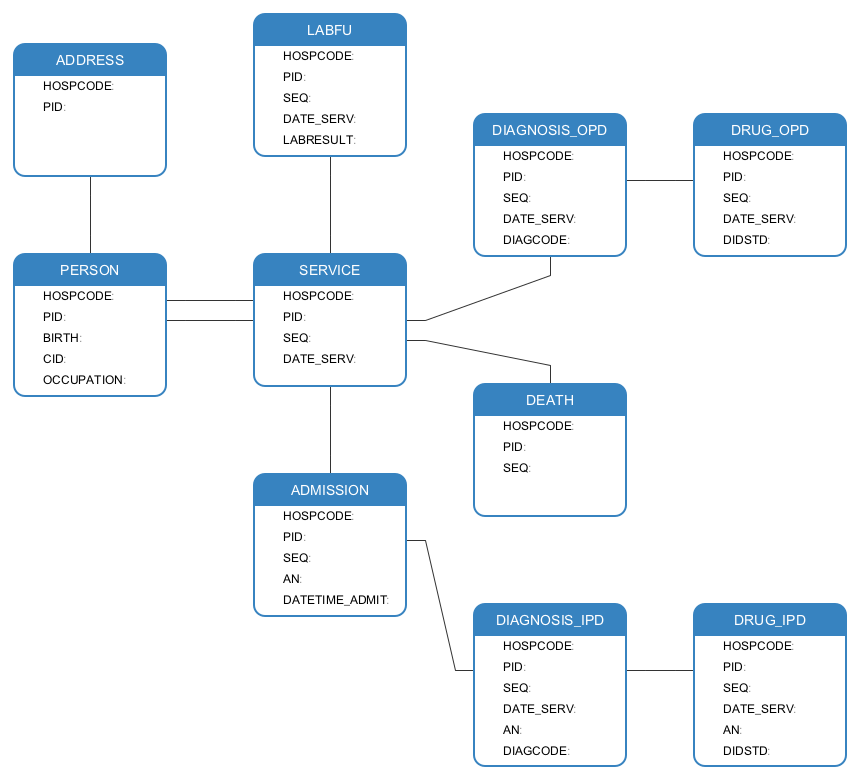
\includegraphics[width=\linewidth]{images/chapter-04/43-folders-relationship.png}
            	\caption{43 Folder Relationship}
        		\label{figure-43-folder-relationship}
        \end{figure}
        \FloatBarrier

\section{How the Data Flow} \label{section:how-the-data-flow}
    % (2014 up to now) 946GB++
    % Intro
    To begin with, there are four main areas that the data goes through which are Hospital, Provincial Public Health Office(PHO), Ministry of Public Health-ICT(MoPH-ICT), and Bureau of Policy and Strategy(BPS) as shown in figure \ref{fig_data_flow1}. First of all, the data start at the hospital area when staff have to record their patient information when patient walk in to the hospital and check  by using the program that they have in order to record. This step is shown in number one in figure \ref{fig_data_flow1}. After finish the first phase, hospital have to send the data or we known as "43 file" to PHO in less than or equal 1 month. It mean that staff at hospital have to send the data to PHO every month as it shown in number two in figure \ref{fig_data_flow3}. Then the staff at PHO will verify the data that is sent by hospital, and then they will report the data  that have error back to hospital in order to review and fix the data. Every day the staff at PHO have to send the summary data such as record of patient that visit to hospital to MoPH-ICT. Also, PHO have to send 43-file to MoPH-ICT in every 15 days as it shown in figure \ref{fig_data_flow3}, then the staff of MoPH-ICT have to update data that they receive from PHO in a day. After that, the data will be updated to the system as show in number 4 in figure \ref{fig_data_flow4}, then the system will use that data to analysis and visualize the report to web-application as it shown in number 4 in figure \ref{fig_data_flow4}. In addition, the last area is BPS where the system will get the dead data that we are missing. The data that come in to the system do not cover all dead data, it include only dead data that patient who die in hospital, but it is not include the patient who die outside the hospital, so we have to make a request to get the missing dead data at BPS. However, we can not conclude yet that how we will get the data from BPS, it is still in the processing of discussion to find the way to get the dead data.

    \FloatBarrier
        \begin{figure}[h!]
            \centering
                % can use width=\linewidth
            	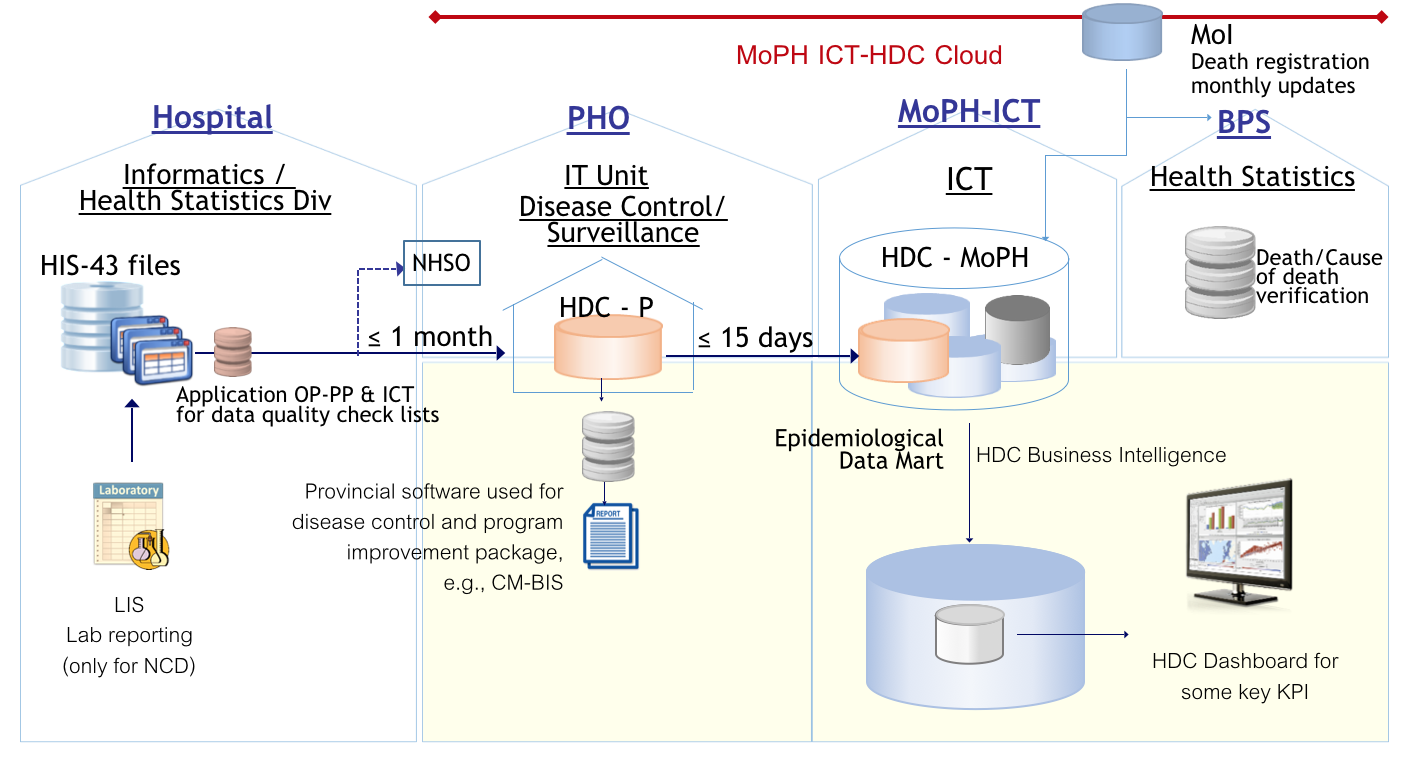
\includegraphics[width=9cm]{images/chapter-04/data_flow1.png}
            	\caption{Data Flow 1}
            	\label{fig_data_flow1}
        \end{figure}
    \FloatBarrier
    \FloatBarrier
        \begin{figure}[h!]
            \centering
                % can use width=\linewidth
            	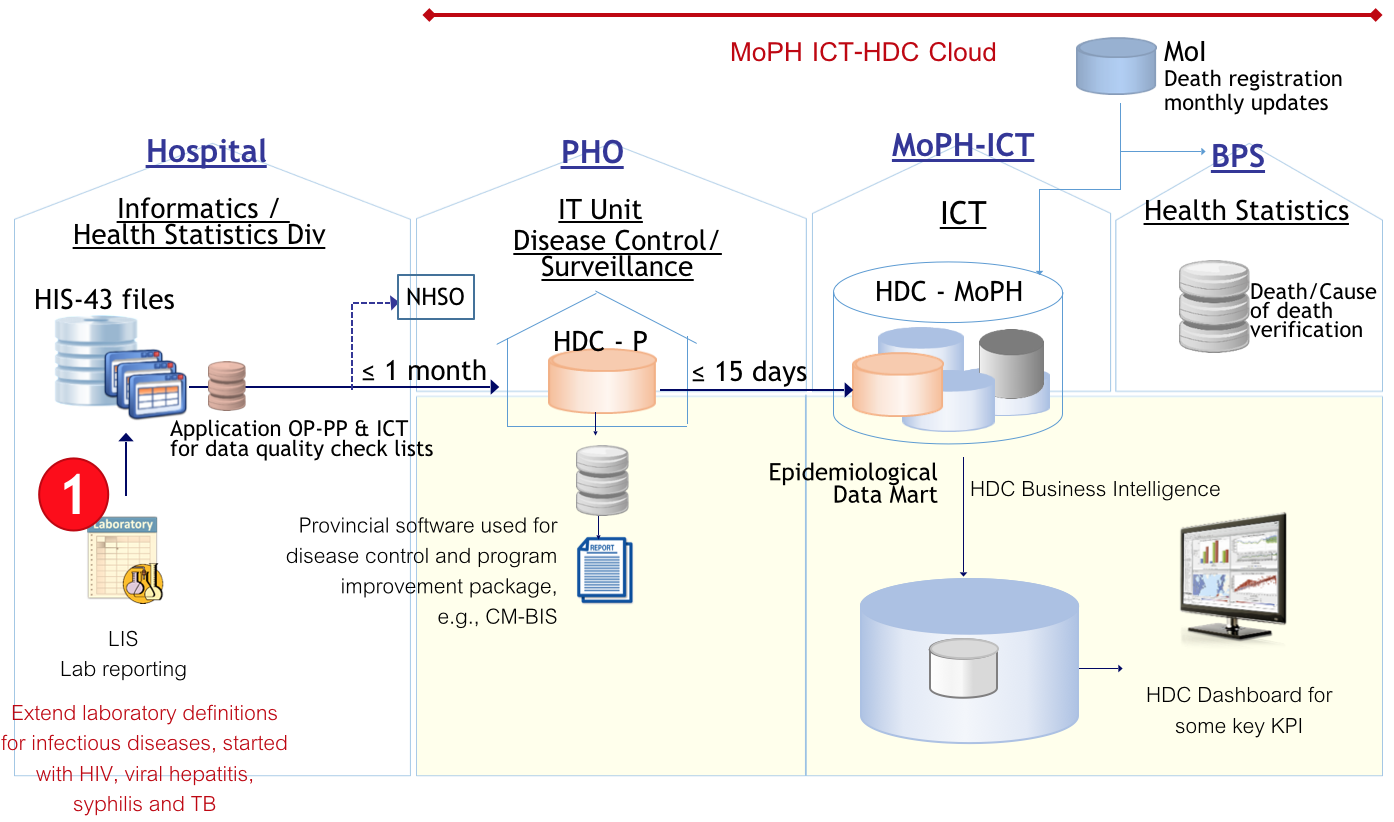
\includegraphics[width=9cm]{images/chapter-04/data_flow2.png}
            	\caption{Data Flow 2}
            	\label{fig_data_flow2}
        \end{figure}
    \FloatBarrier
    \FloatBarrier
        \begin{figure}[h!]
            \centering
                % can use width=\linewidth
            	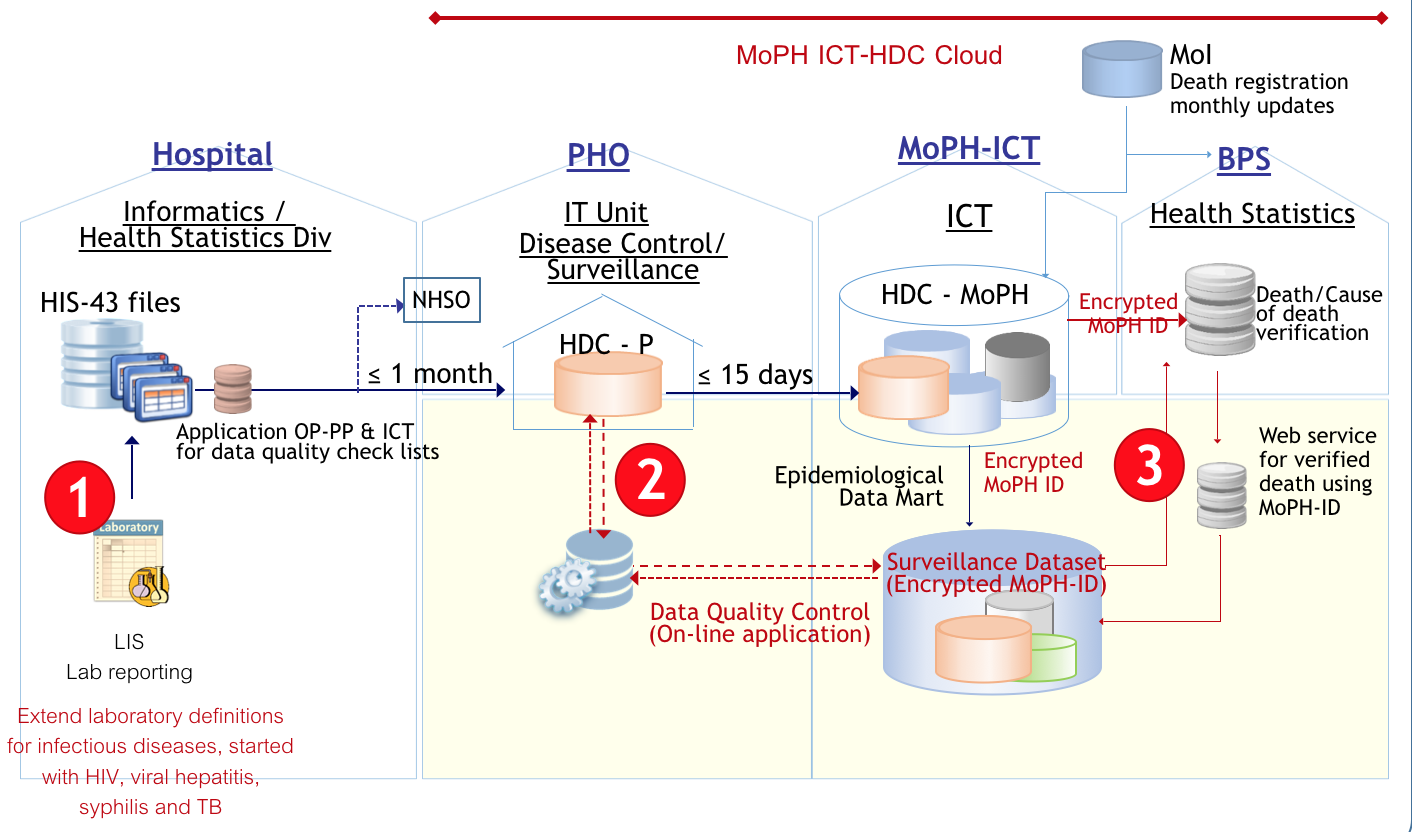
\includegraphics[width=9cm]{images/chapter-04/data_flow3.png}
            	\caption{Data Flow 3}
            	\label{fig_data_flow3}
        \end{figure}
    \FloatBarrier
    \FloatBarrier
        \begin{figure}[h!]
            \centering
                % can use width=\linewidth
            	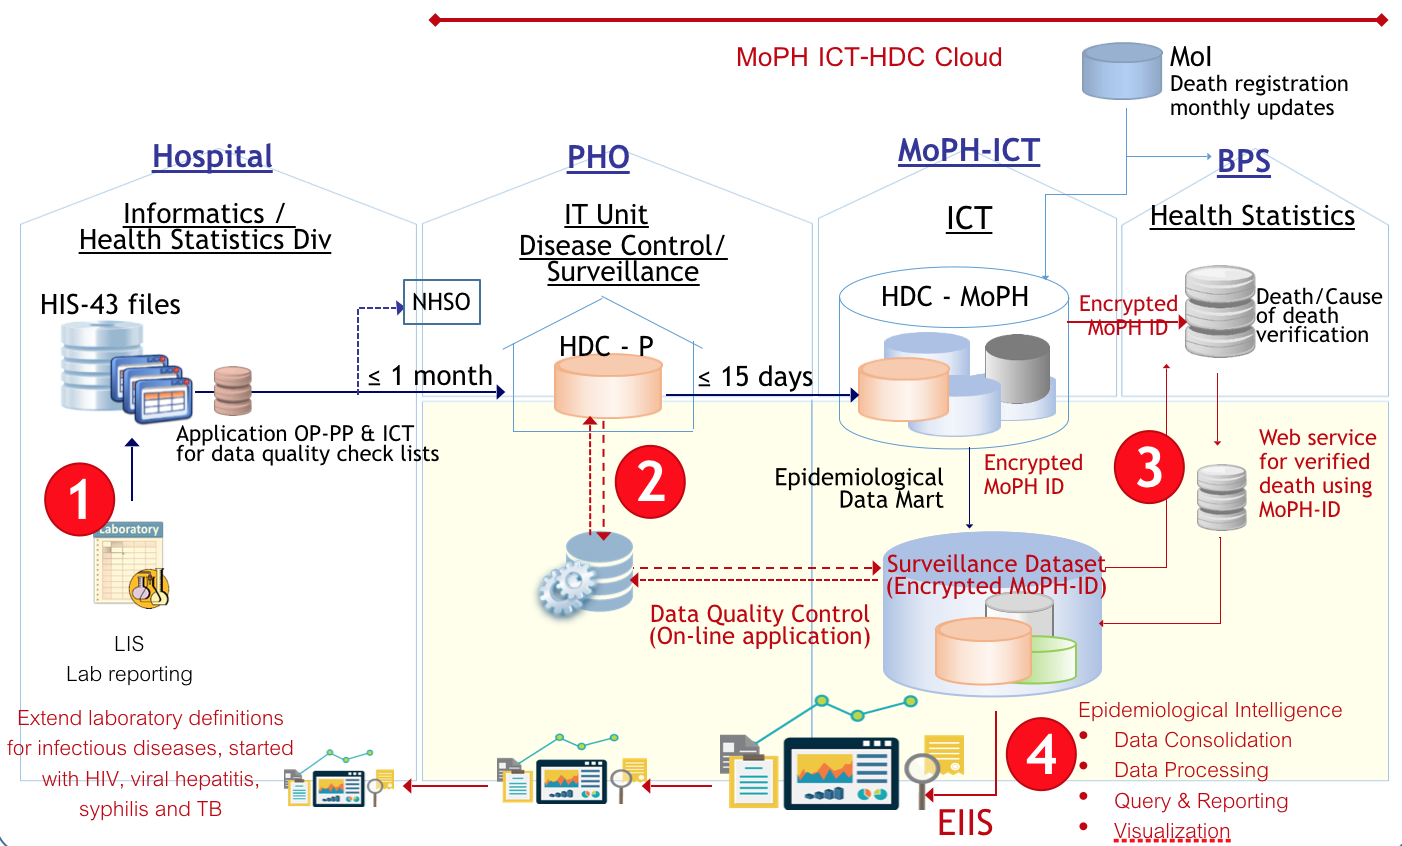
\includegraphics[width=9cm]{images/chapter-04/data_flow4.png}
            	\caption{Data Flow 4}
            	\label{fig_data_flow4}
        \end{figure}
    \FloatBarrier
    
% death แจ้งผู้ใหญ่บ้าน
    \chapter{Frontend Implementation}

\section{Architecture Overview}
    There are many reasons why we chose React in our project. First of all, everything in React is component which it consists of state (mutable) and props (immutable). It means that it will make your code more predictable and easier to debug. Another reason is that it uses virtual Document Object Model (virtual DOM) instead of using pure DOM. The virtual DOM help to re-render in an efficient way of the DOM. In addition, React will create virtual DOM in memory when the program work, React will renders only the sub-component that only change. 
    


\section{Implementation}
    
    \subsection{Logging into the System}
    
    User can log-in to the application by entering user name ans password, that provided by the developer team, as shown in the figure \ref{log-in}. After entering all user name and password, user have to click log-in button in order to enter to the application. Then the system will send user's credential to validate with server by using POST method to post /api/v1/auth/login with the data to server. If user succeed log-in, at a glance report page will be rendered as shown in figure \ref{at-a-glance-report}. Server will send the data of that user and cookie to the front-end part.
    
    
    \FloatBarrier
    	\begin{figure}[h!]
            \centering
                % can use width=\linewidth
        		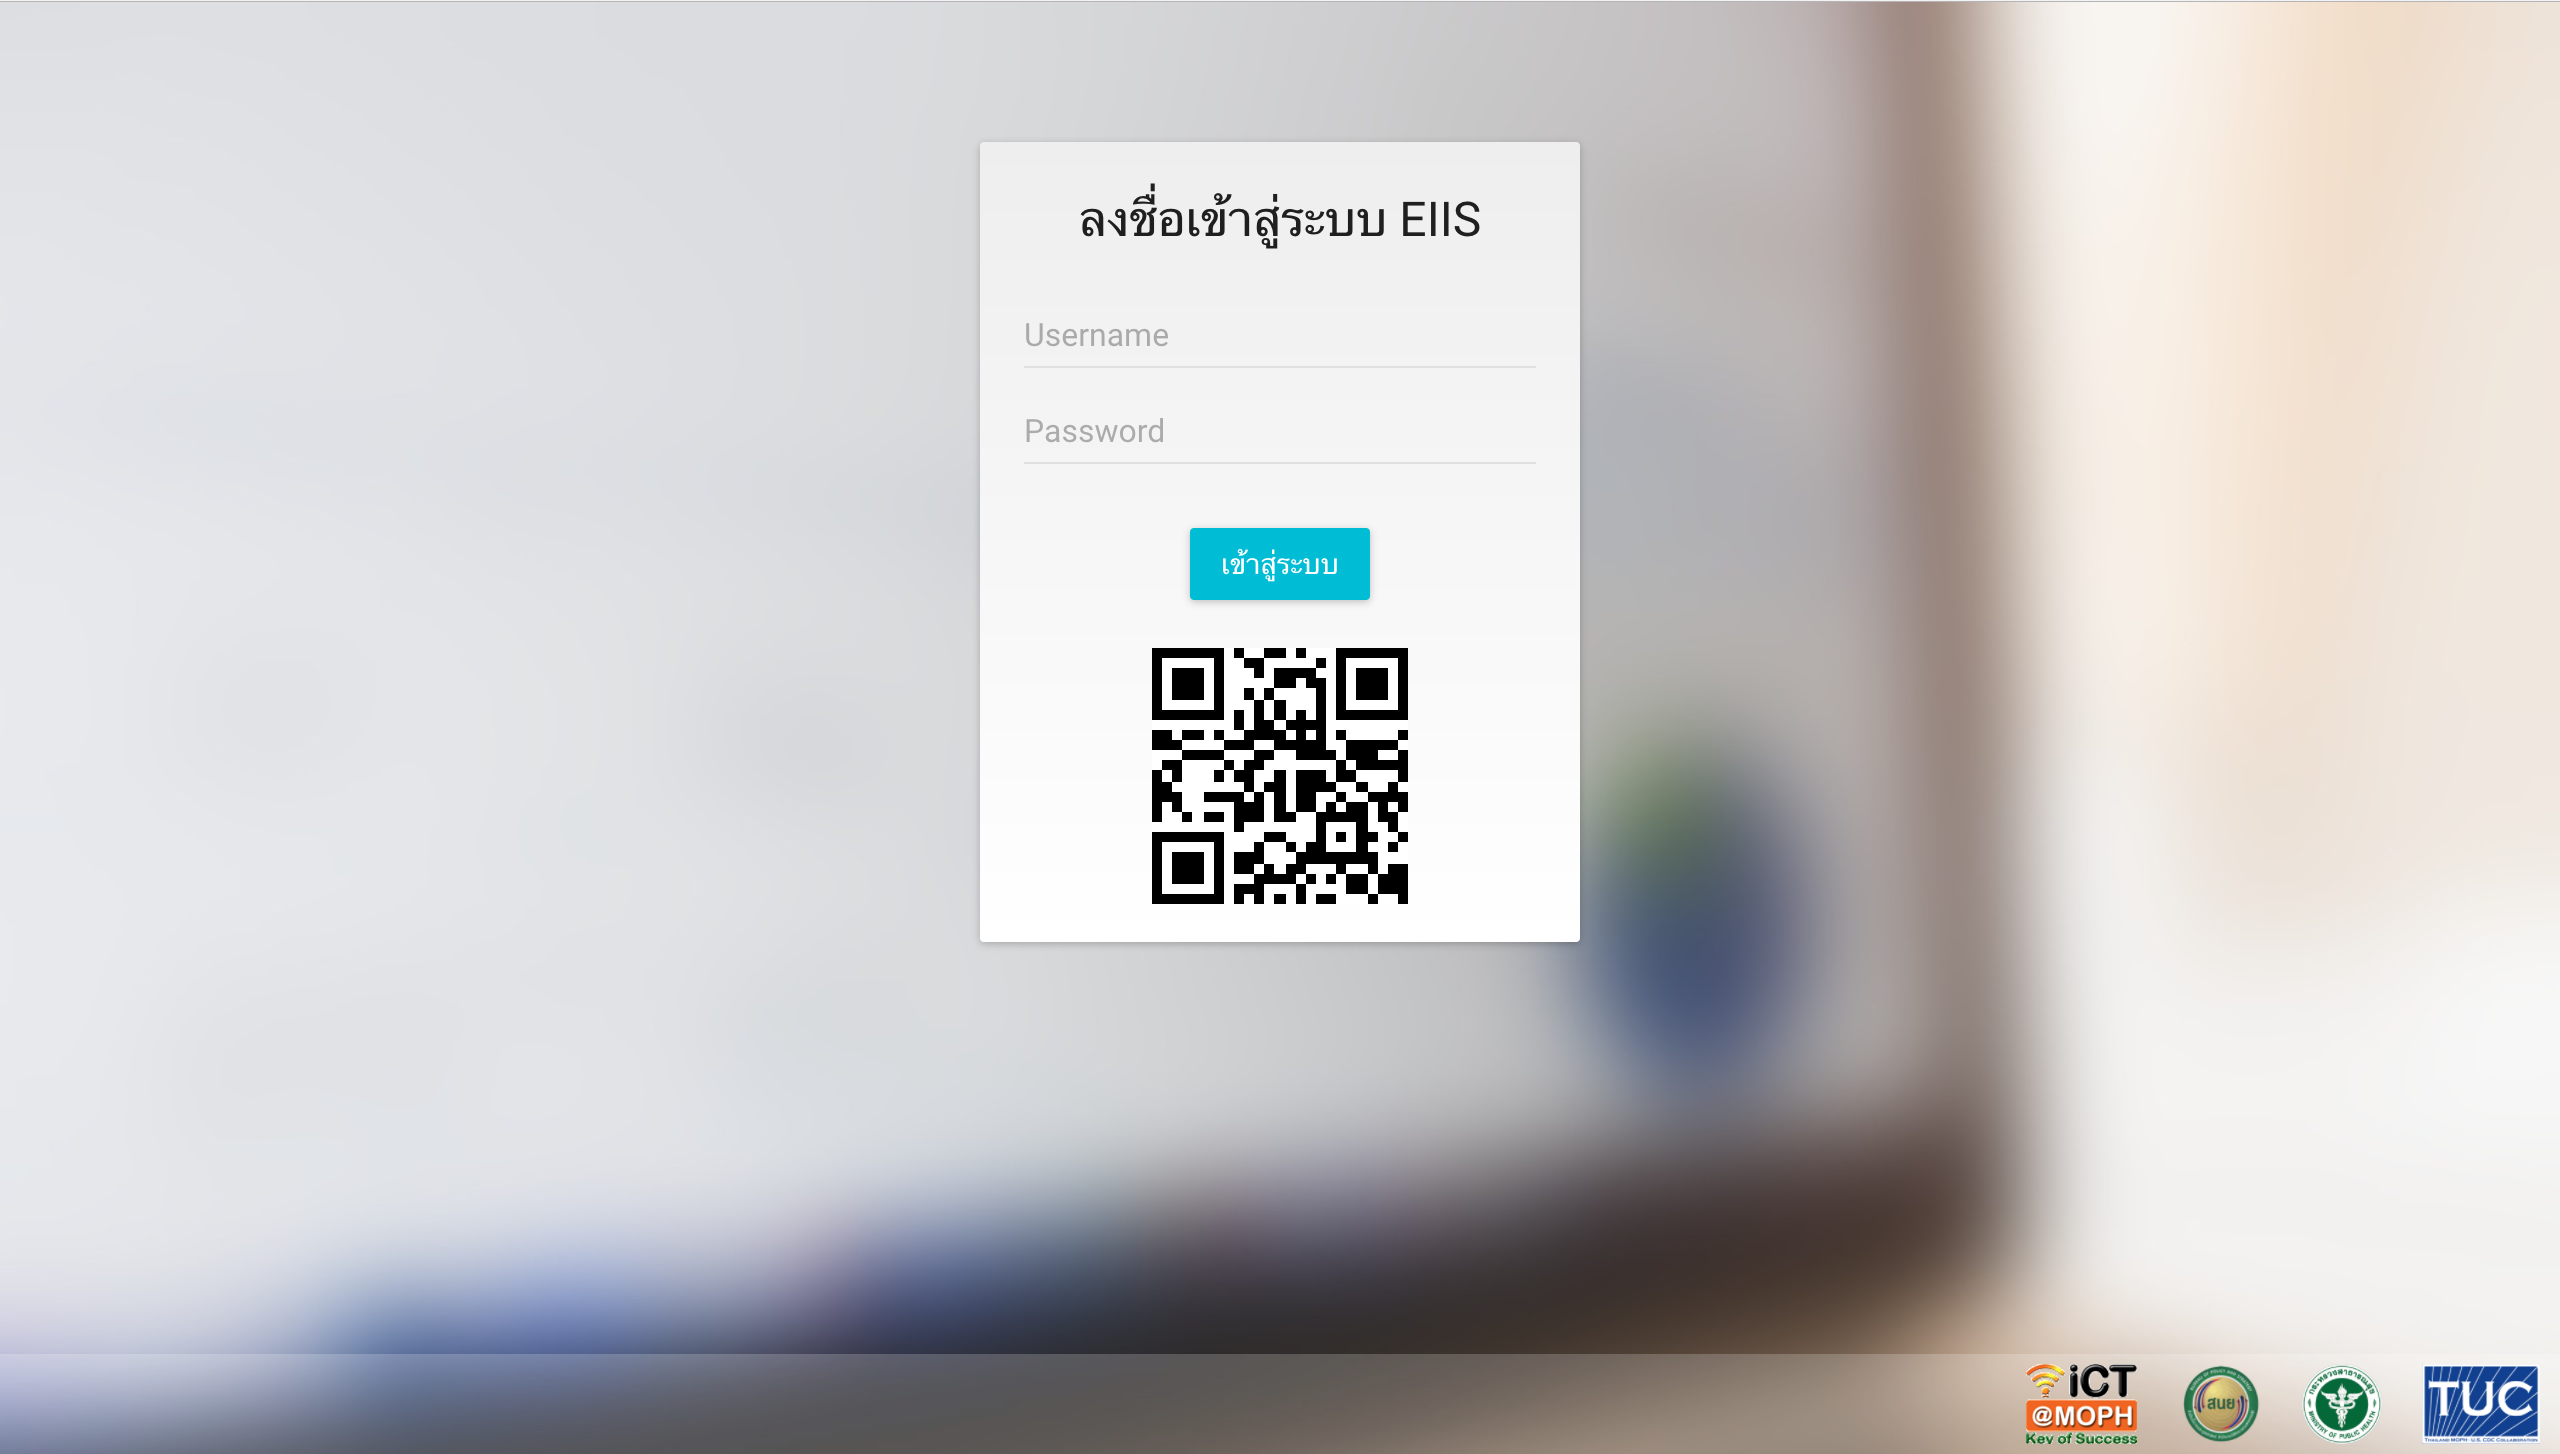
\includegraphics[width=12cm]{images/chapter-05/log-in.png}
        		\caption{Log-In Page}
        		\label{log-in}
        \end{figure}
	\FloatBarrier
	
	
	\subsection{Tab Bar Menu}
	
	This is all the menus that user can click to go to those pages. There are several pages in this application such as, home page, upload page, check upload status page, at a glance report page, demographics page, and so on. The tab bar menu shown in figure \ref{tab-bar-menu}
	
	\FloatBarrier
    	\begin{figure}[h!]
            \centering
                % can use width=\linewidth
        		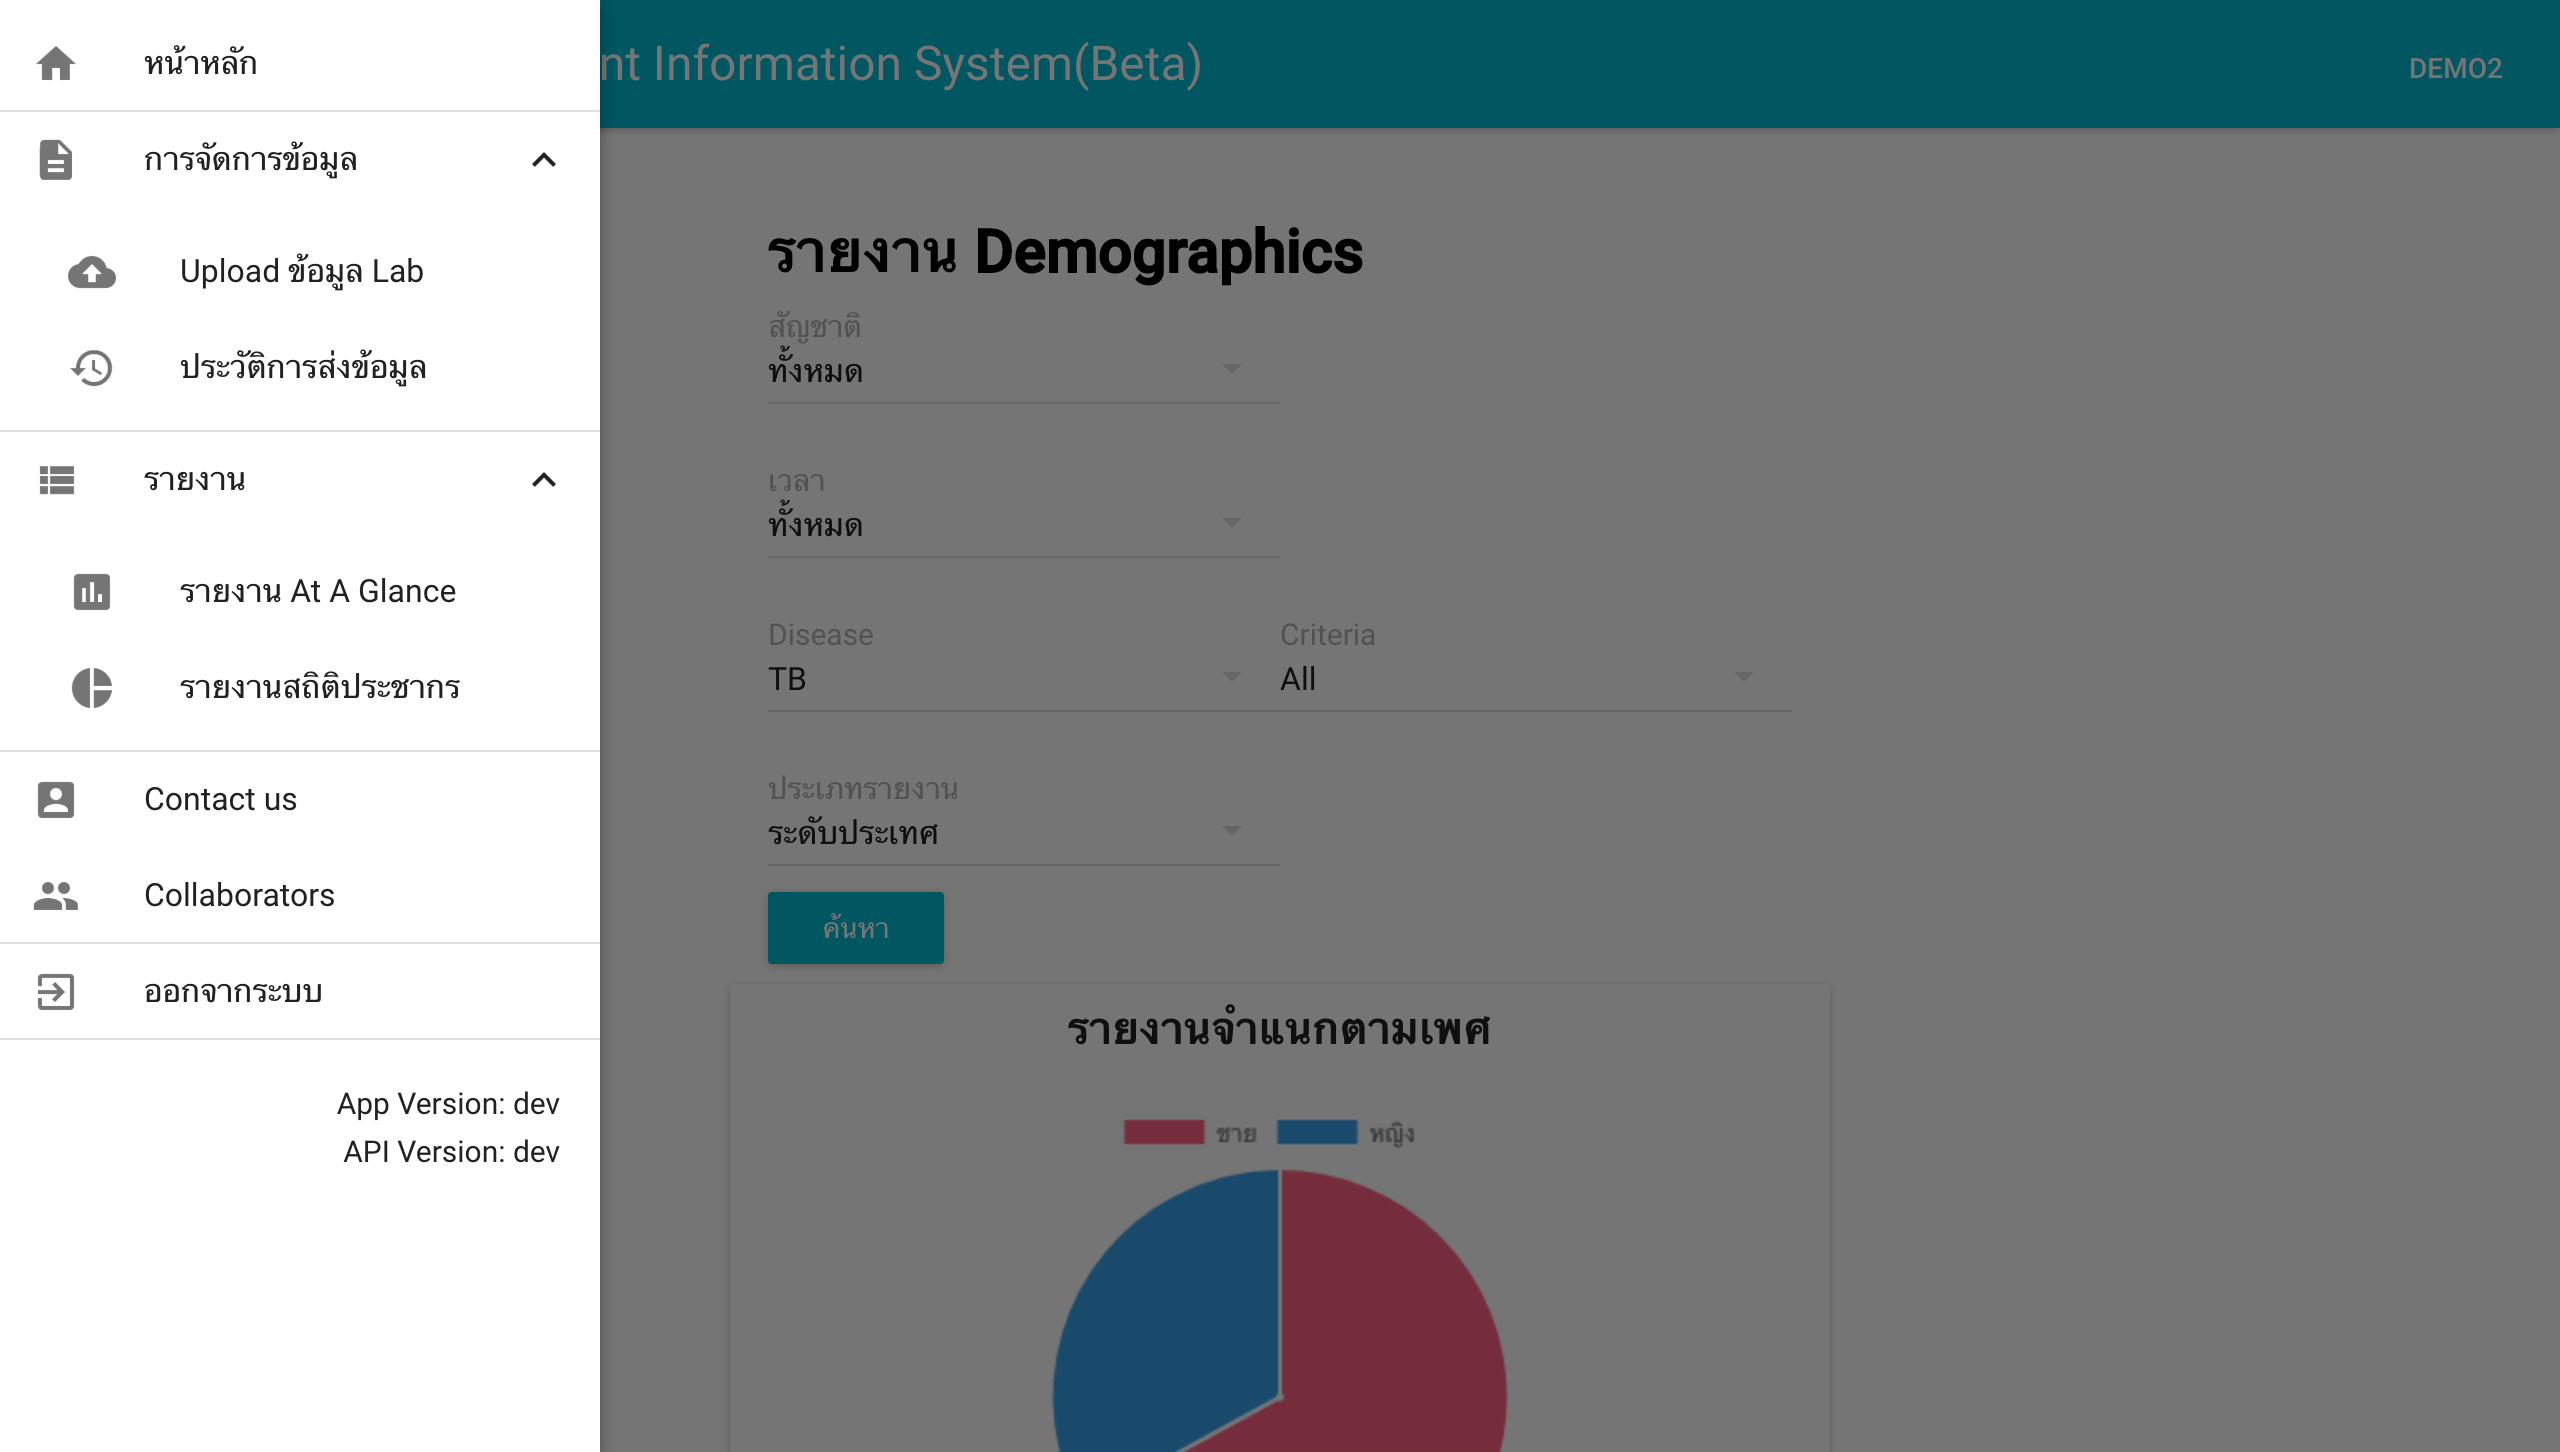
\includegraphics[width=12cm]{images/chapter-05/tab-bar-menu.png}
        		\caption{Menus}
        		\label{tab-bar-menu}
        \end{figure}
	\FloatBarrier
	
	\subsection{At a Glance Report}
	
	To see at a glance report, user need to select at a glance report in tab bar menu as shown in figure \ref{tab-bar-menu} or it will show you immediately when you log-in to the system. Then, user can select type of data that they want by selecting time, disease, criteria of the disease, and the type of report that they want. In order to see all the drop-down select, there are in section \ref{filter-data}. When user finished selecting, user need to click 'find' button as shown in figure \ref{at-a-glance-report}. Then the front-end will send the input data to the server via POST. For example, api/v1/hiv/at-a-glance/all. Then the server will send json object back, then the table will be rendered as shown in figure \ref{at-a-glance-report}. 
	
	
    \FloatBarrier
    	\begin{figure}[h!]
            \centering
                % can use width=\linewidth
        		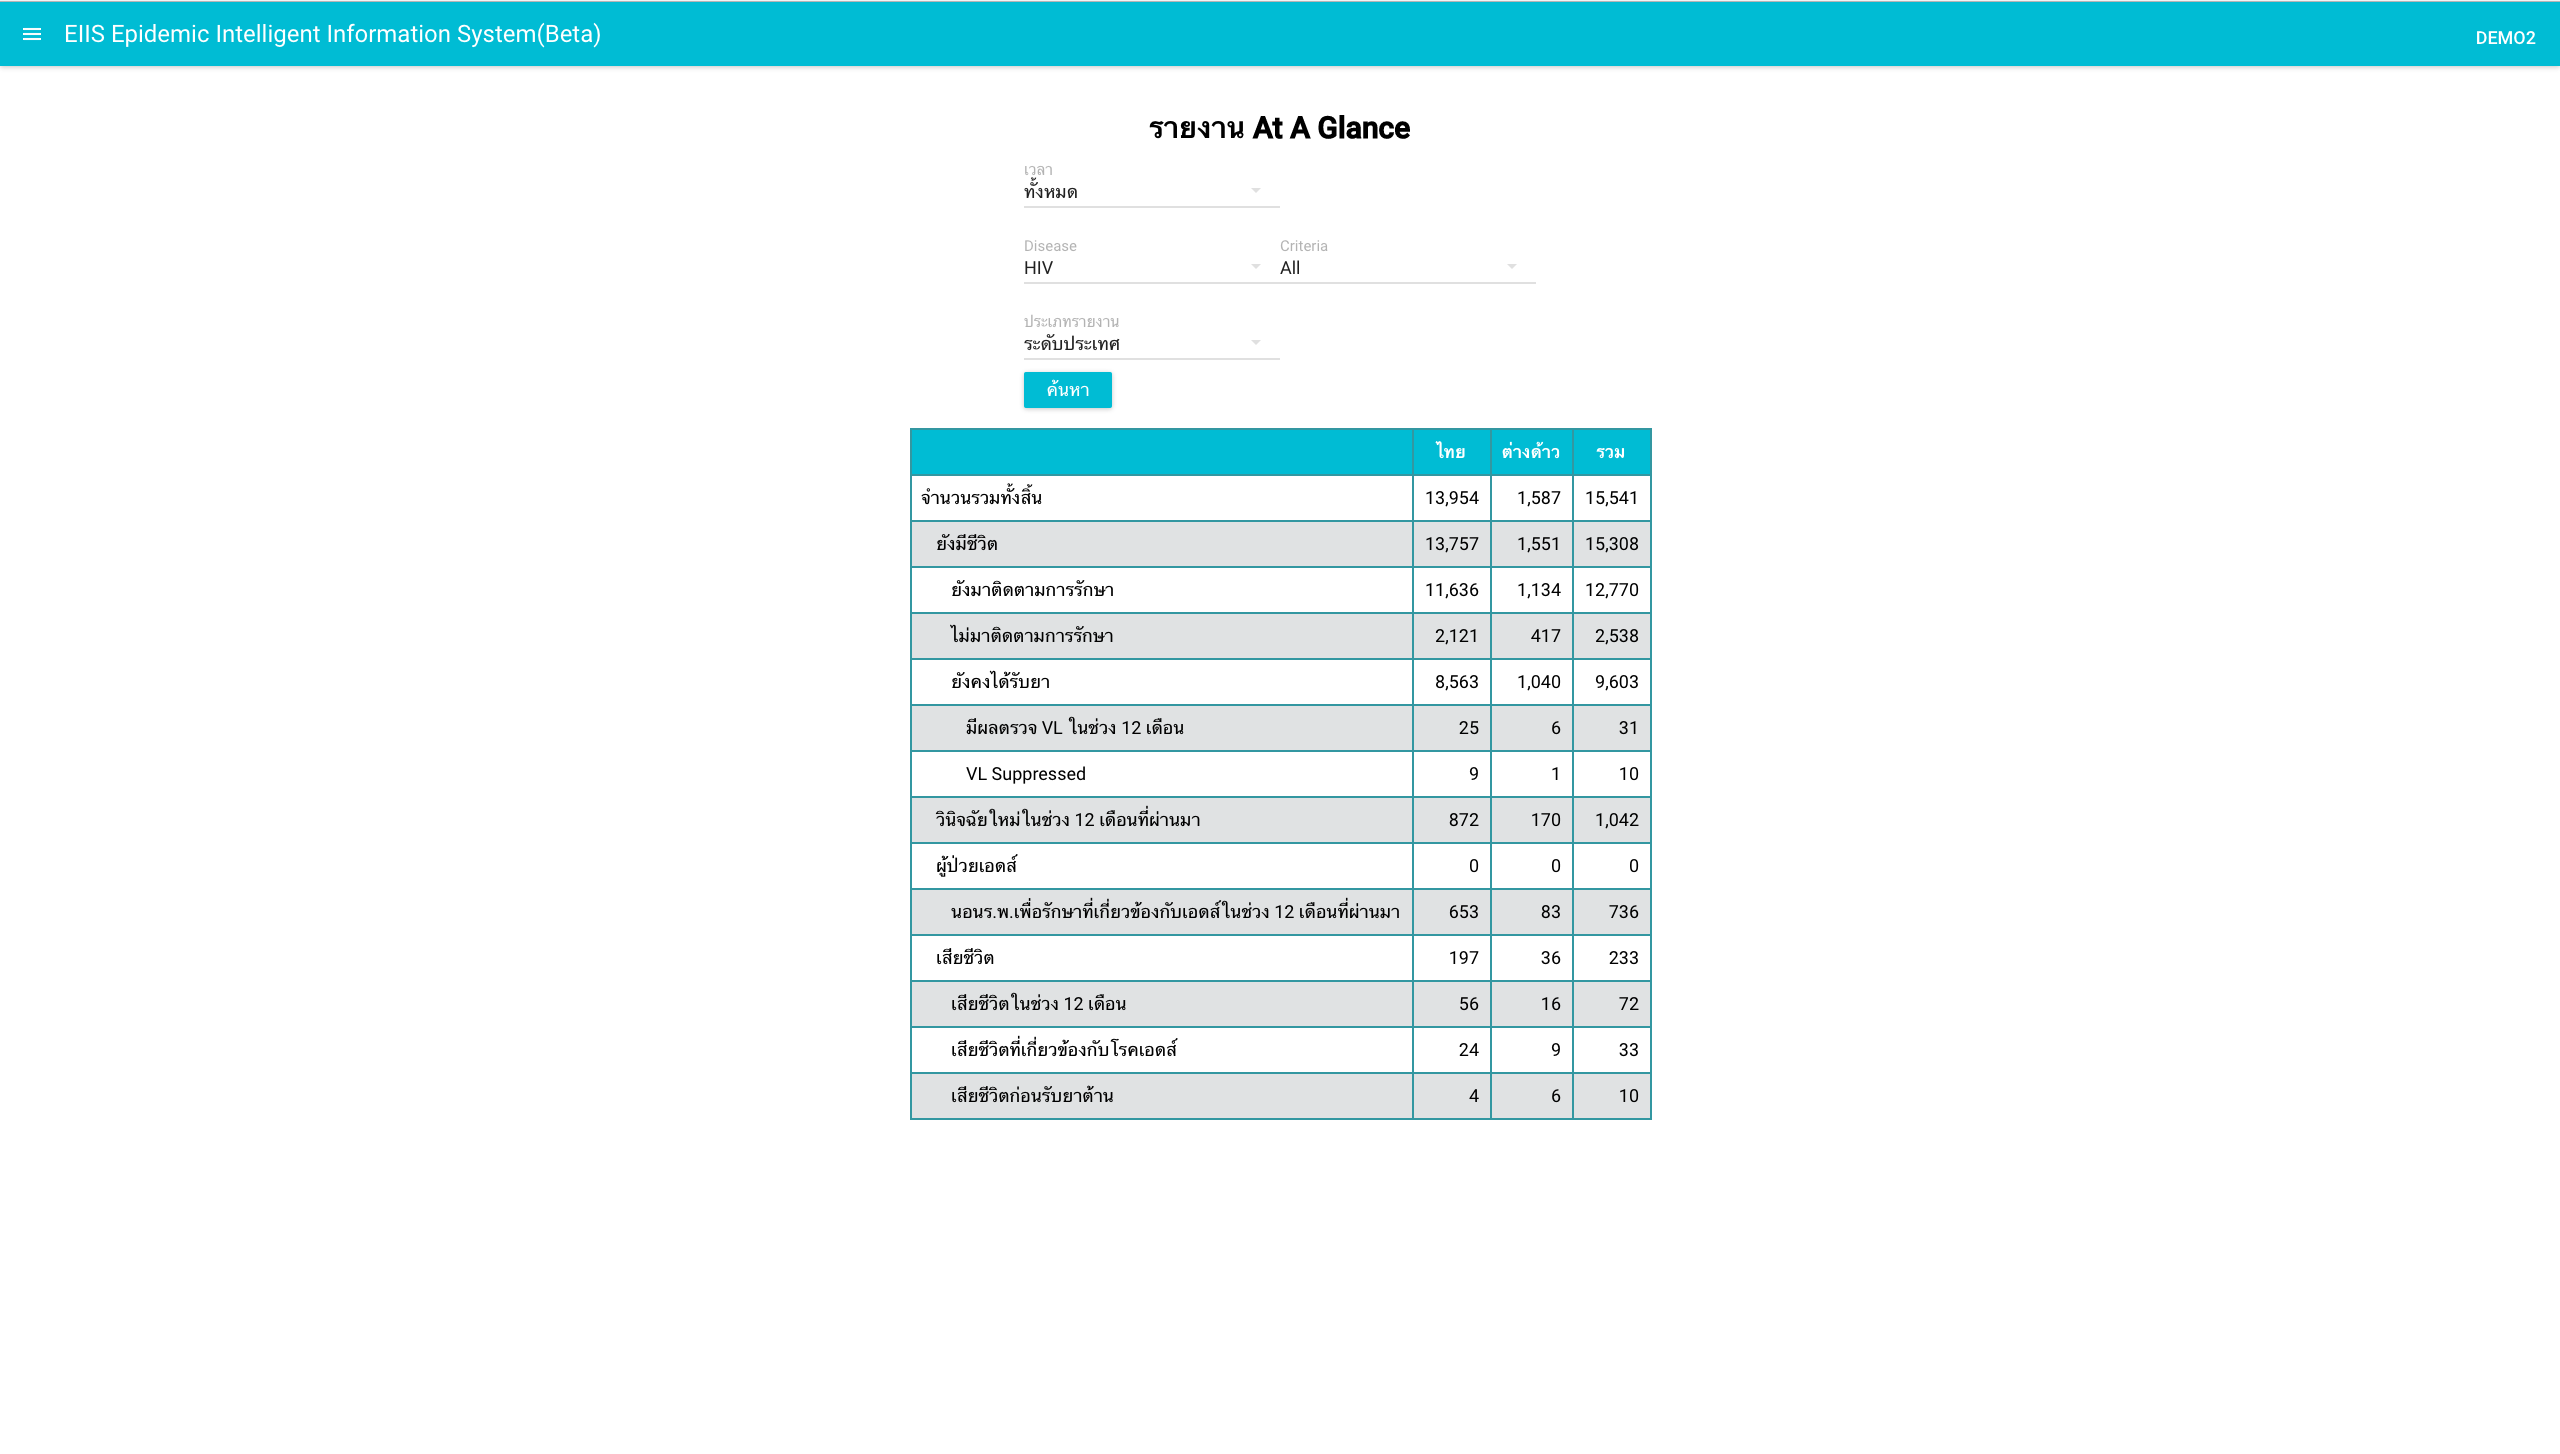
\includegraphics[width=12cm]{images/chapter-05/at-a-glance-report.png}
        		\caption{At a Glance Report}
        		\label{at-a-glance-report}
        \end{figure}
	\FloatBarrier
	

	
	\subsection{Upload File} \label{upload_file}
	To upload file to EIIS application, user need to select upload lab file in tab bar menu that shown in figure \ref{tab-bar-menu}. Then, user need to select hospital(it will be provides according to the role of that user), month, and year as in figure \ref{upload-status1} then click next to go to another step. In step two, user need to select the file, either file-in or file-out, but at least user need to pick one file in order to upload then click upload button as shown in figure \ref{upload-status2}. After that the front-end will send the data with POST method. For instance, /api/v1/extralab/upload. Next, the server will send the data back to the front-end and shows the data as shown in figure \ref{upload-status3}. In addition, if user do not put any file and click upload button, the upload box will be red ,as shown in figure \ref{upload-error},as warning the user that they have to put some file in order to upload.
   	
   	\vspace{10mm}
    \FloatBarrier
    	\begin{figure}[h!]
            \centering
                % can use width=\linewidth
        		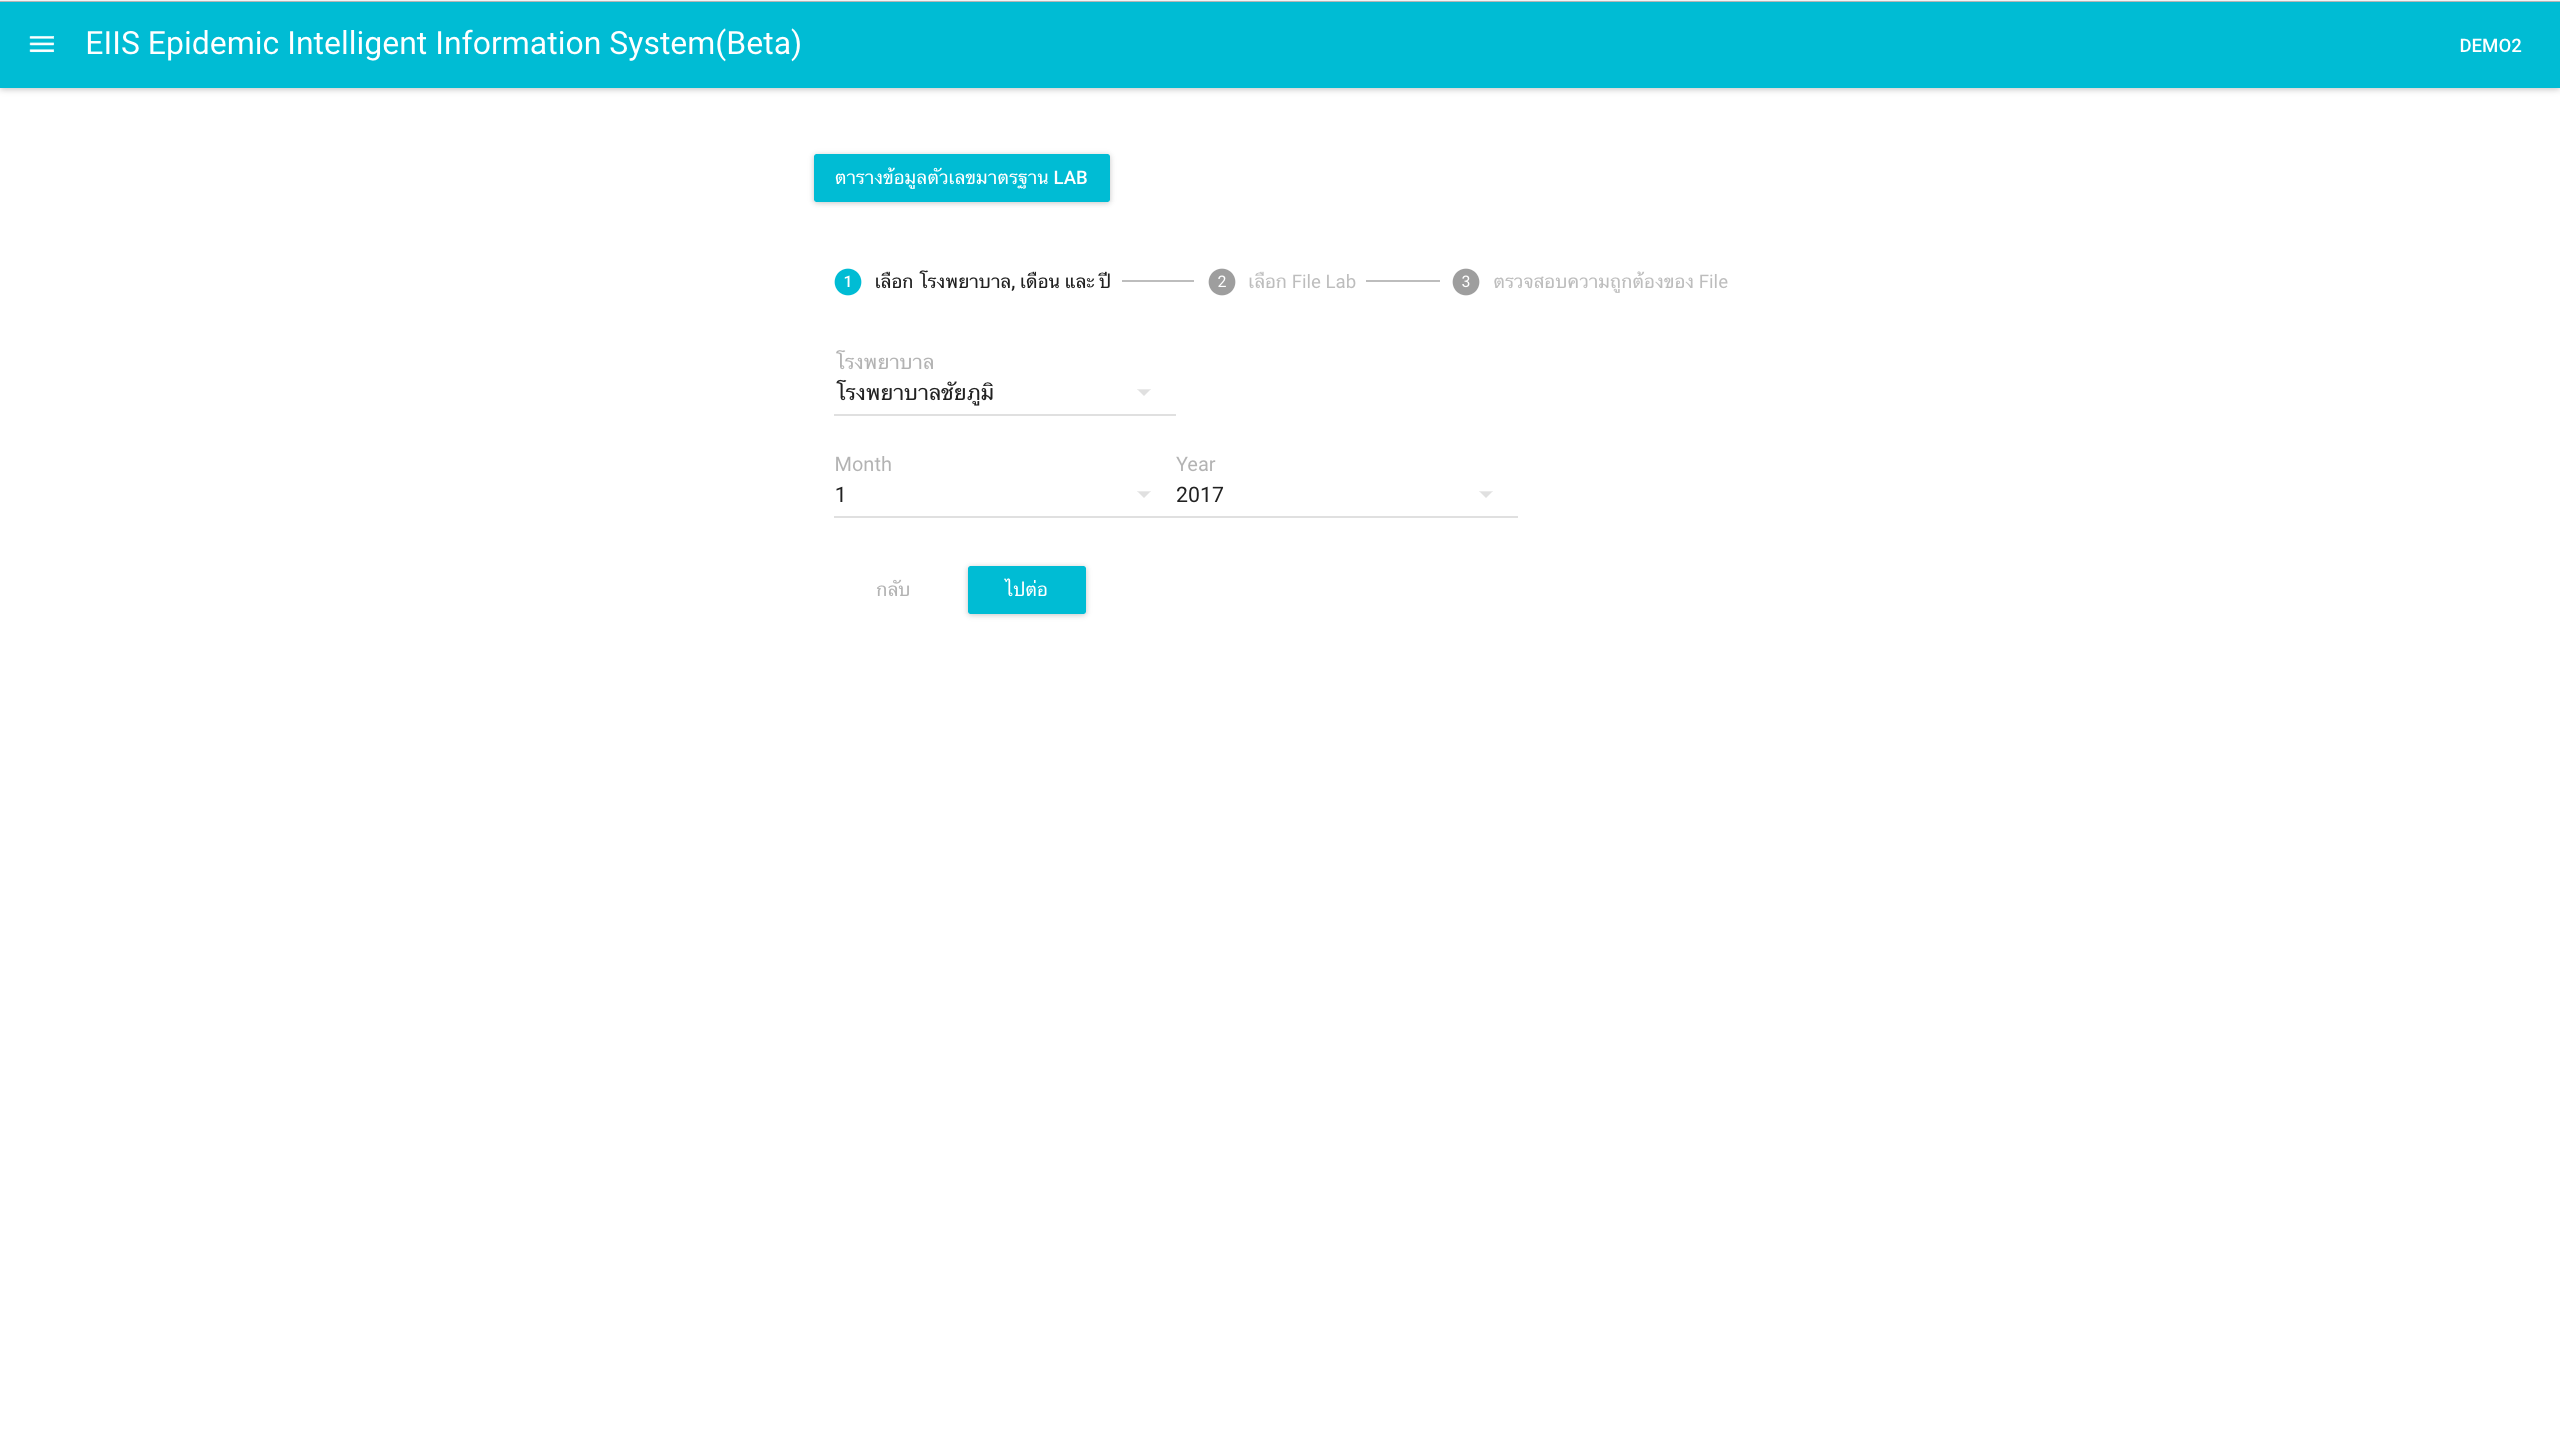
\includegraphics[width=12cm]{images/chapter-05/upload1.png}
        		\caption{Uploading lab file page when user selecting hospital, month, and year}
        		\label{upload-status1}
        \end{figure}
	\FloatBarrier
	
	\FloatBarrier
    	\begin{figure}[h!]
            \centering
                % can use width=\linewidth
        		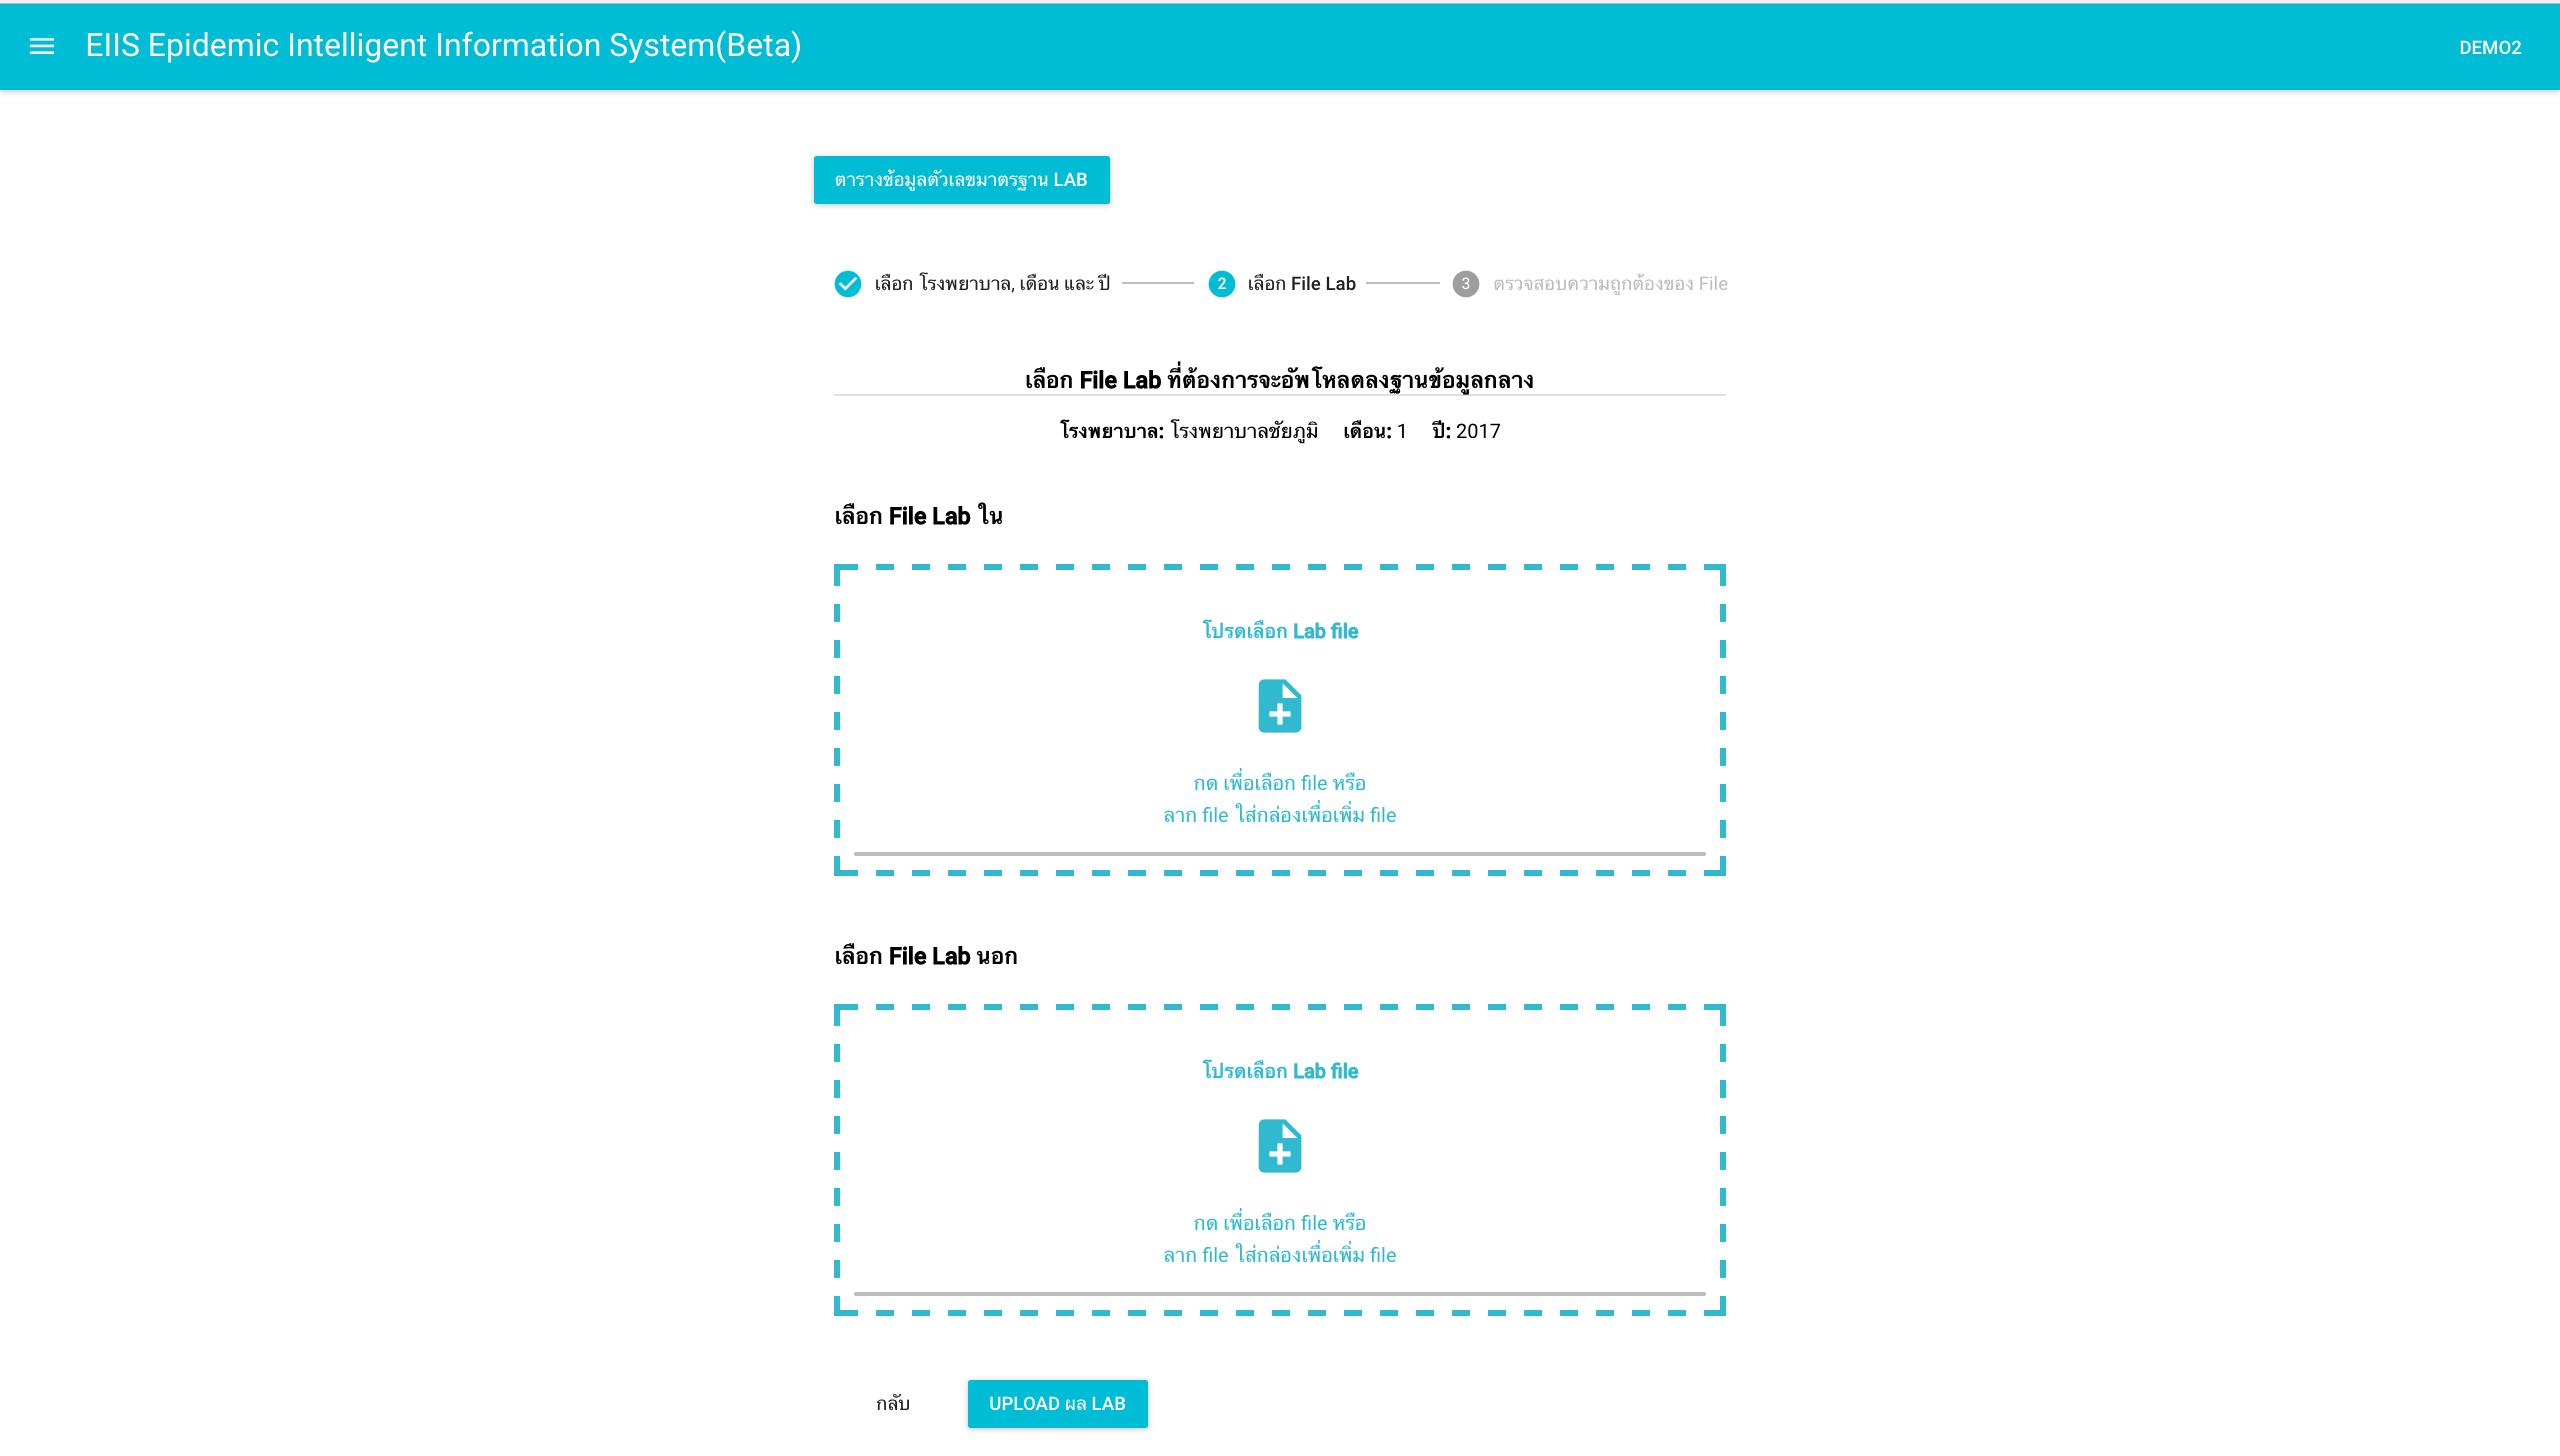
\includegraphics[width=12cm]{images/chapter-05/upload2.png}
        		\caption{Uploading lab file page when user uploading in-patient lab file or out-patien lab file}
        		\label{upload-status2}
        \end{figure}
	\FloatBarrier
	
	\FloatBarrier
    	\begin{figure}[h!]
            \centering
                % can use width=\linewidth
        		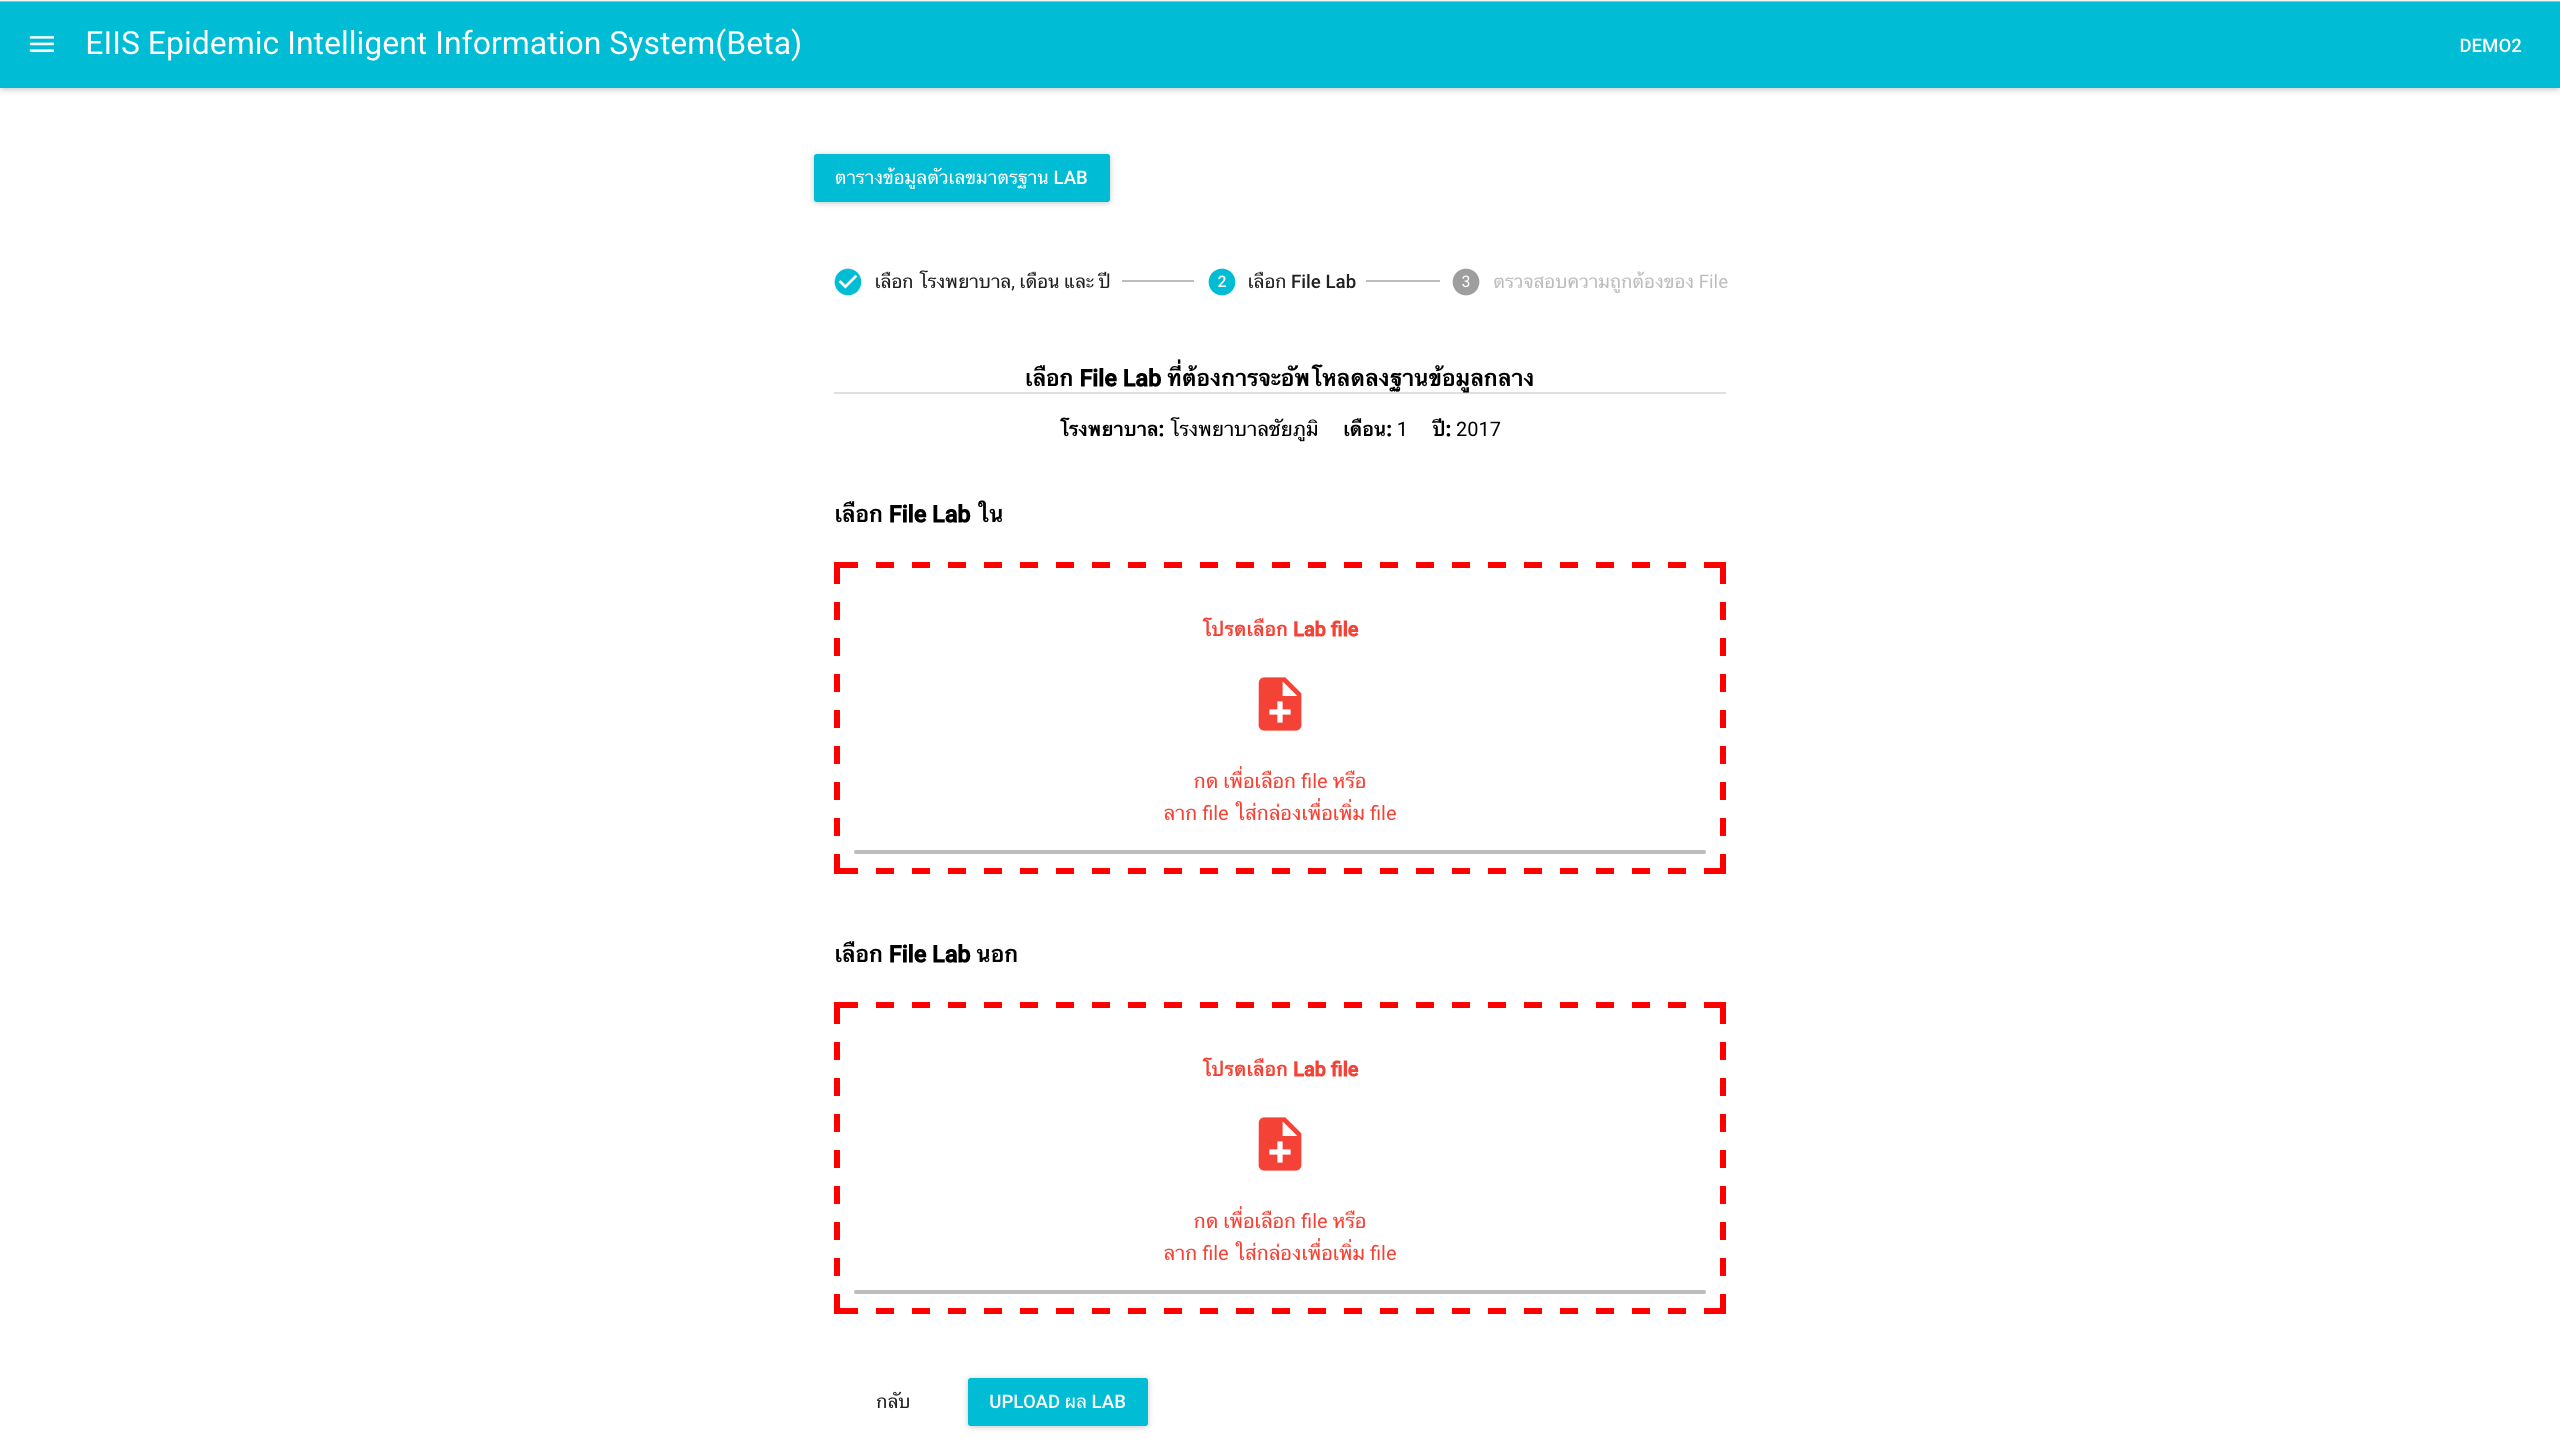
\includegraphics[width=12cm]{images/chapter-05/upload-error.png}
        		% \caption{Upload Error}
        		\caption{Red highlight indicating that the user must select the lab file for uploading to the system}
        		\label{upload-error}
        \end{figure}
	\FloatBarrier
	
	\FloatBarrier
    	\begin{figure}[h!]
            \centering
                % can use width=\linewidth
        		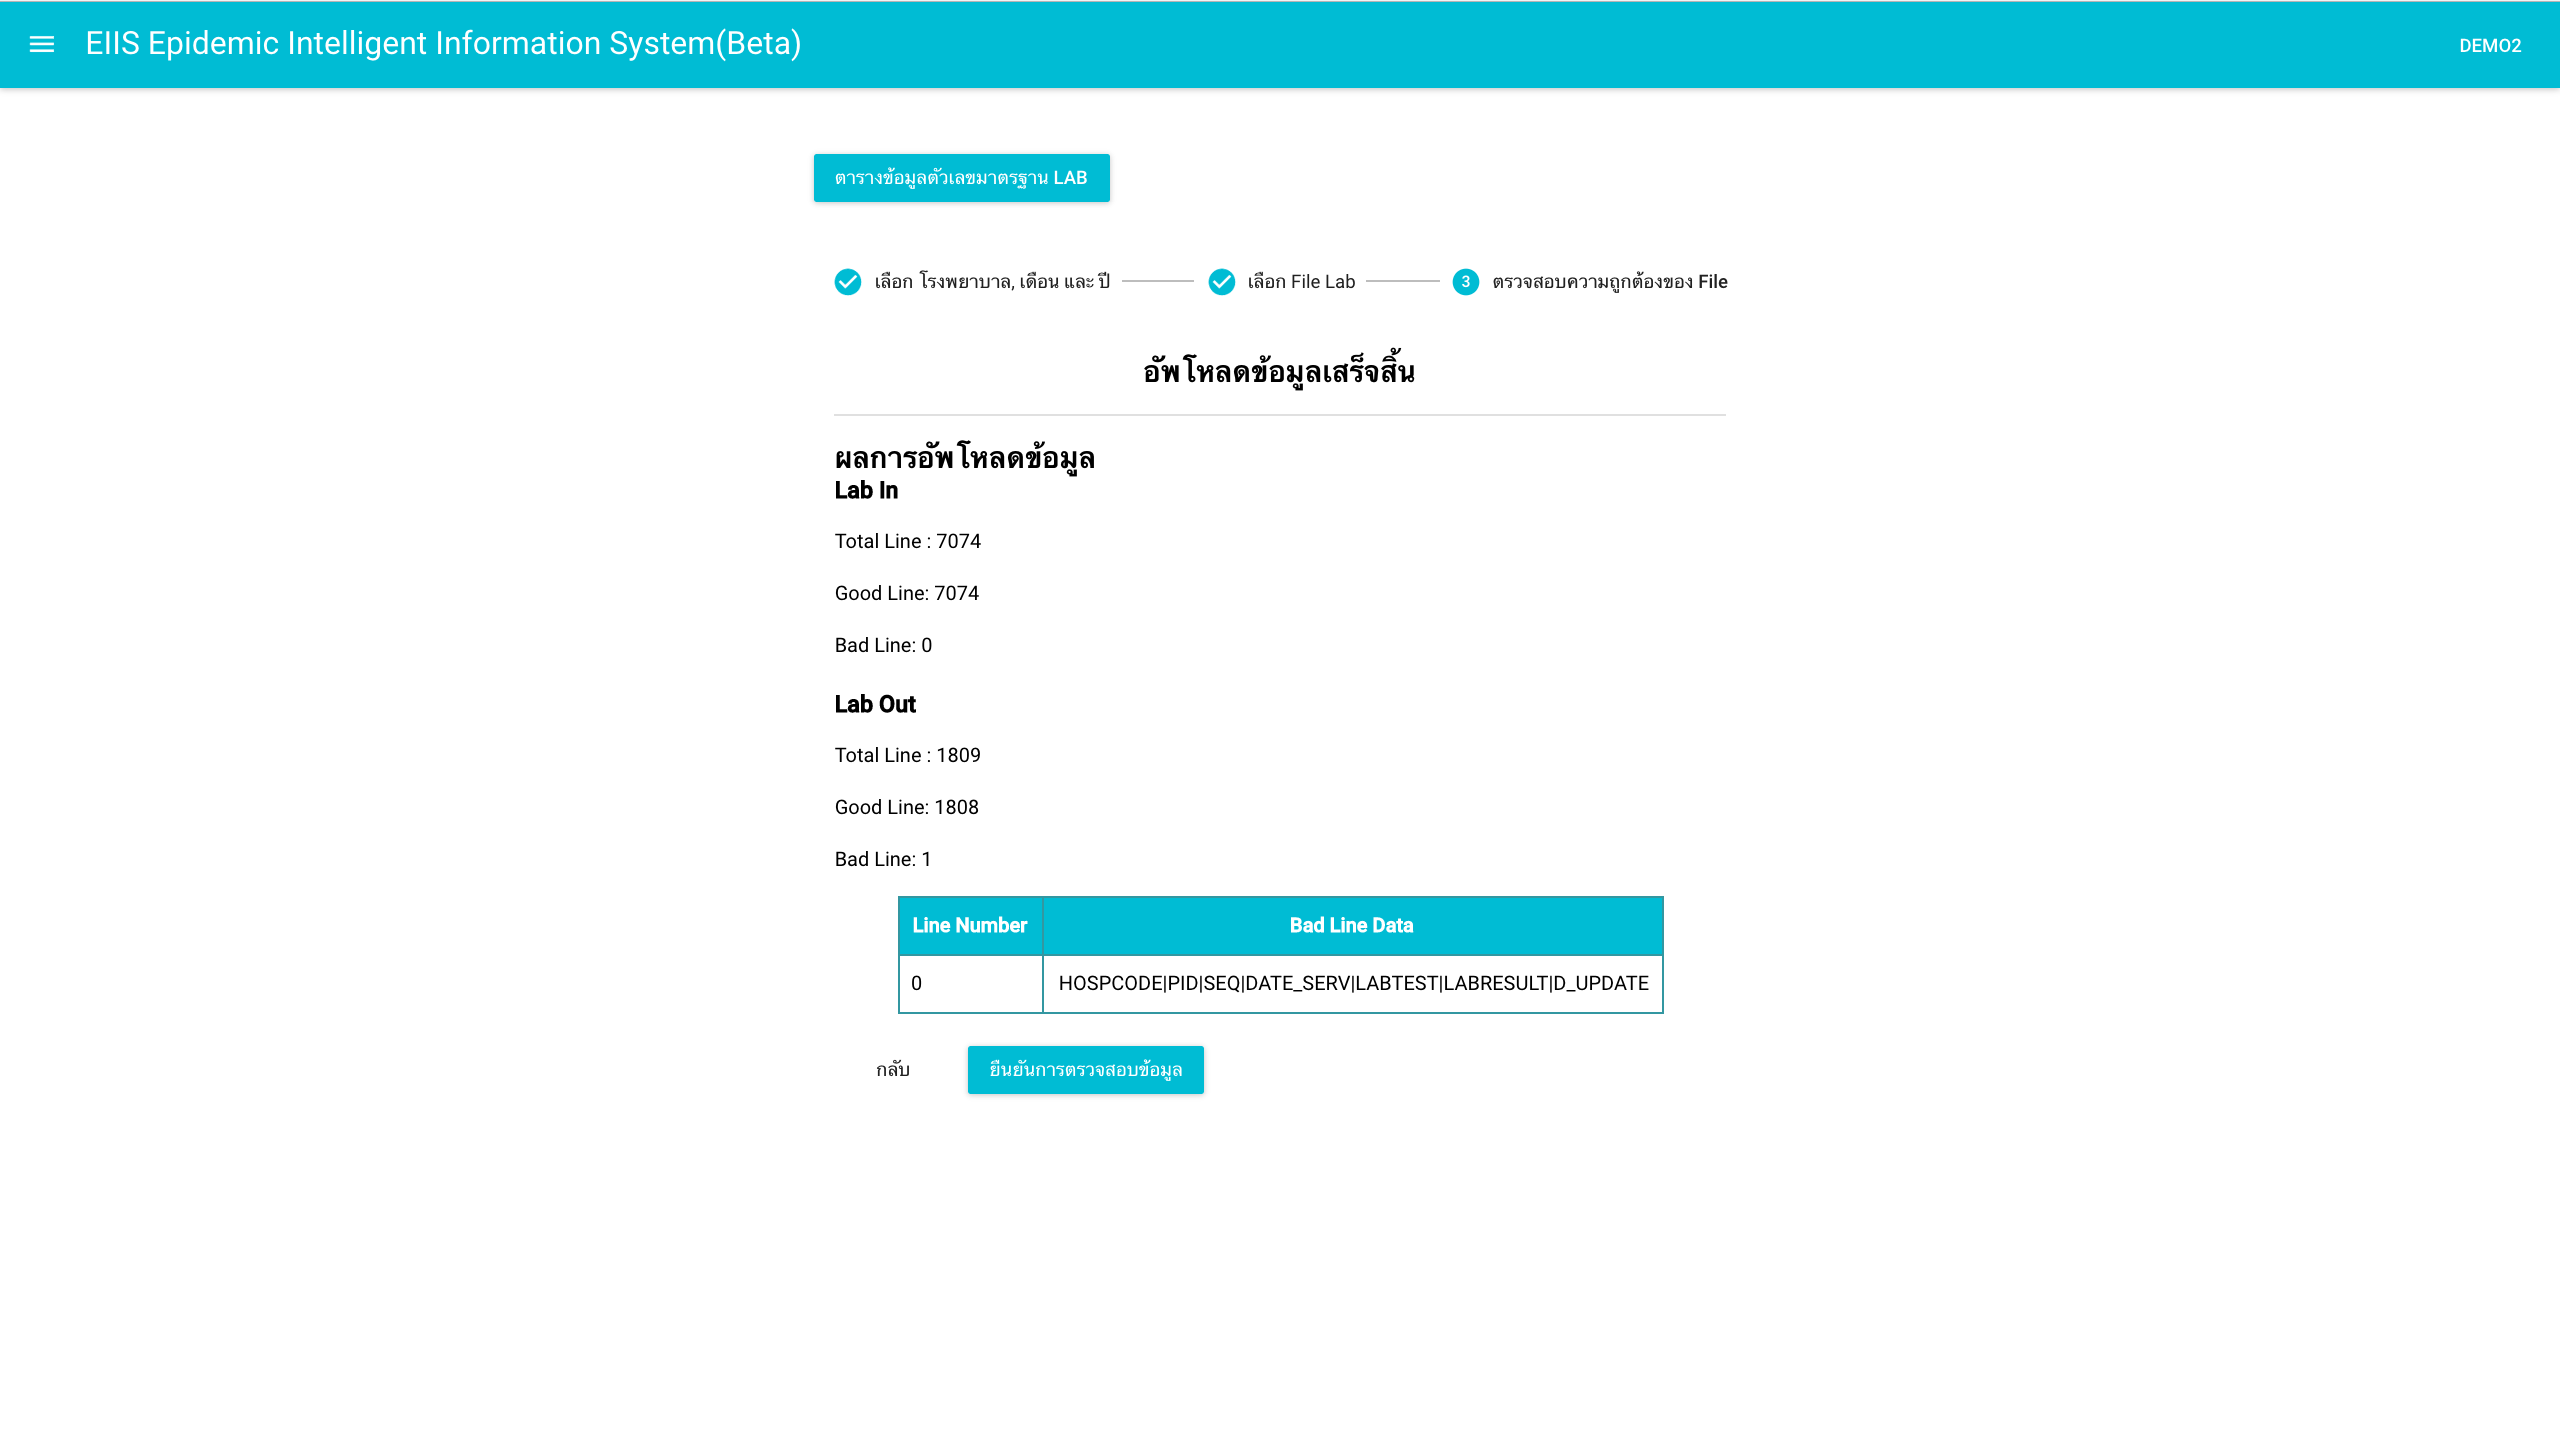
\includegraphics[width=12cm]{images/chapter-05/upload3.png}
        		\caption{Result after user uploading lab file(s)}
        		\label{upload-status3}
        \end{figure}
	\FloatBarrier
	
	
	\subsection{Checking Upload History Status} \label{check_upload_history_status_ui}
% 	/api/v1/extralab/check-status 
	
	To check upload status,user need to select check history of upload file in tab bar menu that shown in figure \ref{tab-bar-menu}. Then, user can select type of report, area, province, and year that they want. In order to see all the drop-down select, there are in section \ref{filter-data}. When user finished selecting, user need to click 'find' button as shown in figure \ref{upload-status0}. The front-end will send the input data to the server via POST. For example, /api/v1/extralab/check-status. After that the server will send json object back, and the table will be rendered as shown in figure \ref{upload-status}. 
	
    \FloatBarrier
    	\begin{figure}[h!]
            \centering
                % can use width=\linewidth
        		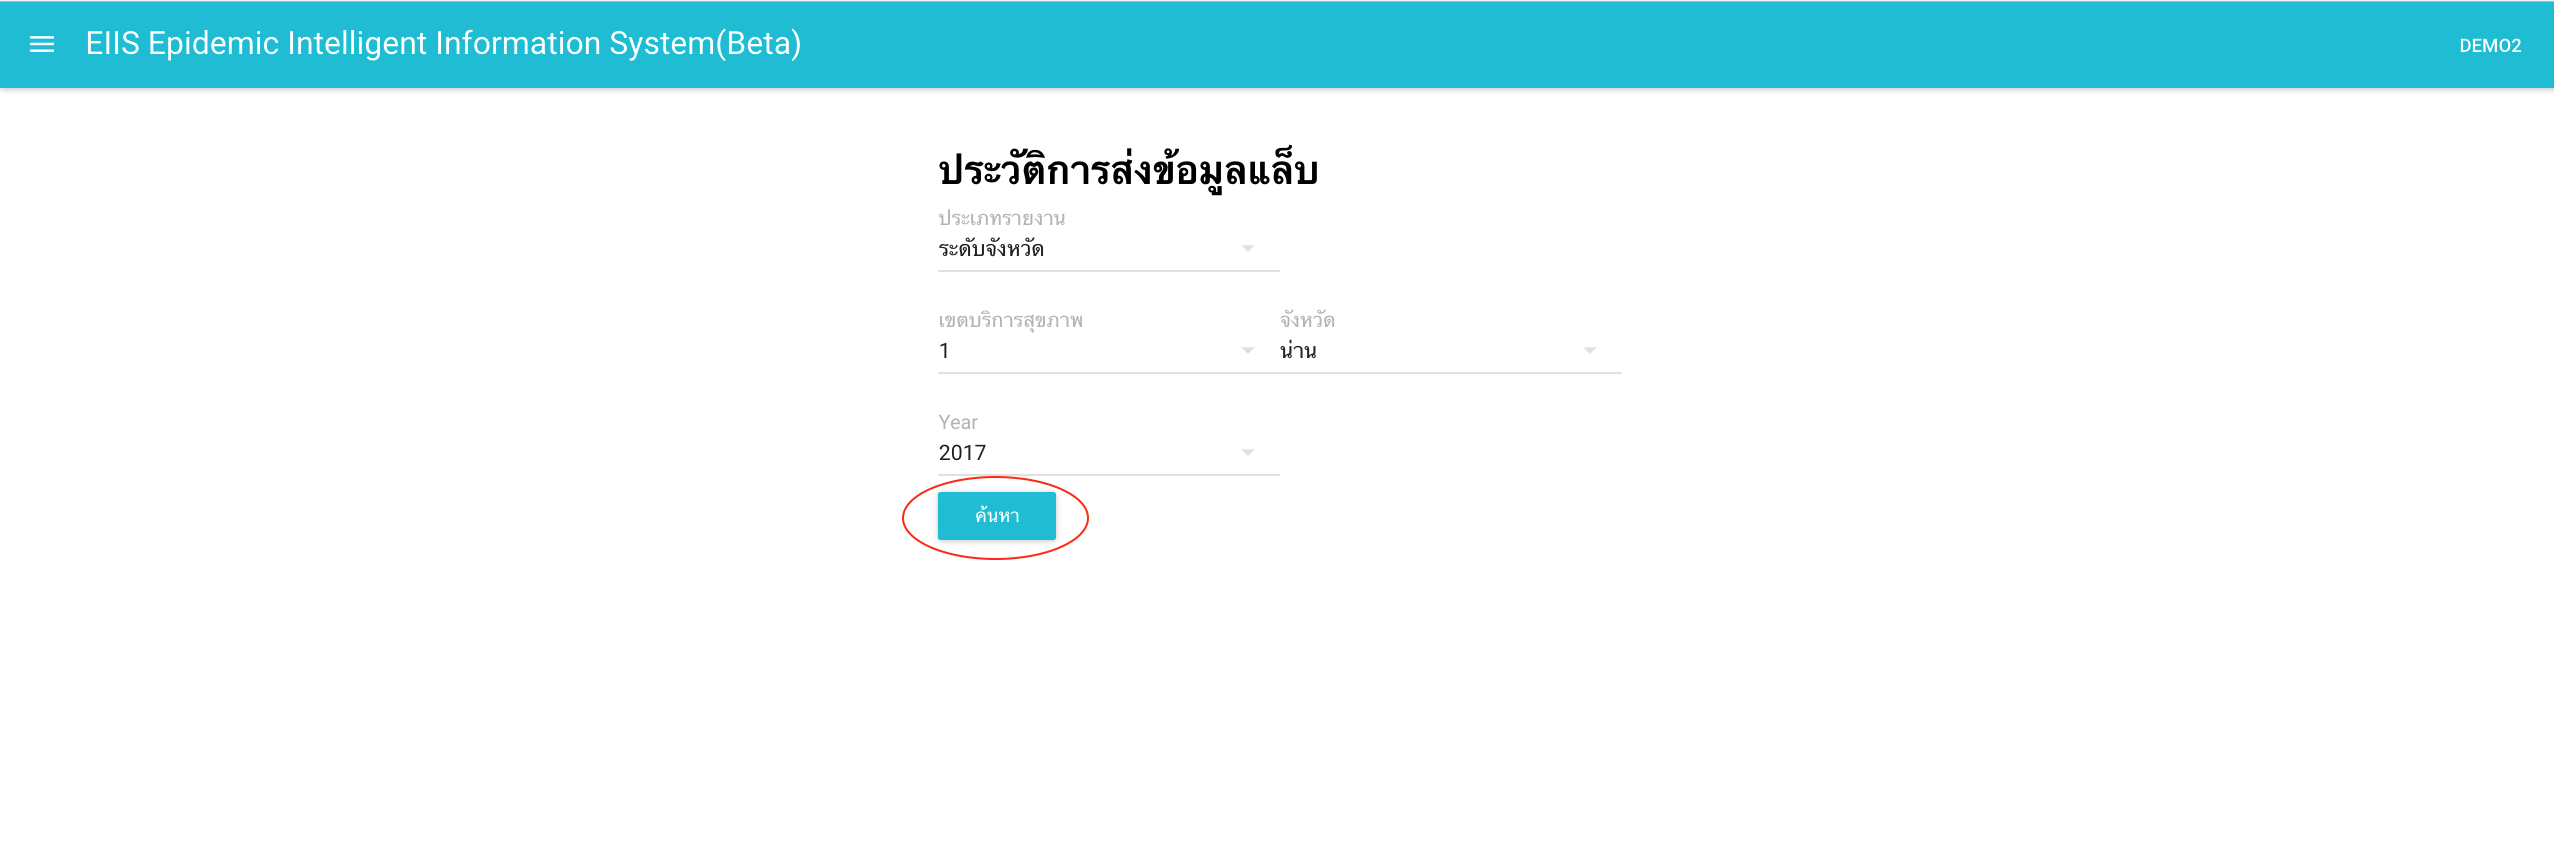
\includegraphics[width=12cm]{images/chapter-05/check-upload-status0.png}
        		\caption{Checking uploaded lab files status}
        		\label{upload-status0}
        \end{figure}
	\FloatBarrier
	
	\FloatBarrier
    	\begin{figure}[h!]
            \centering
                % can use width=\linewidth
        		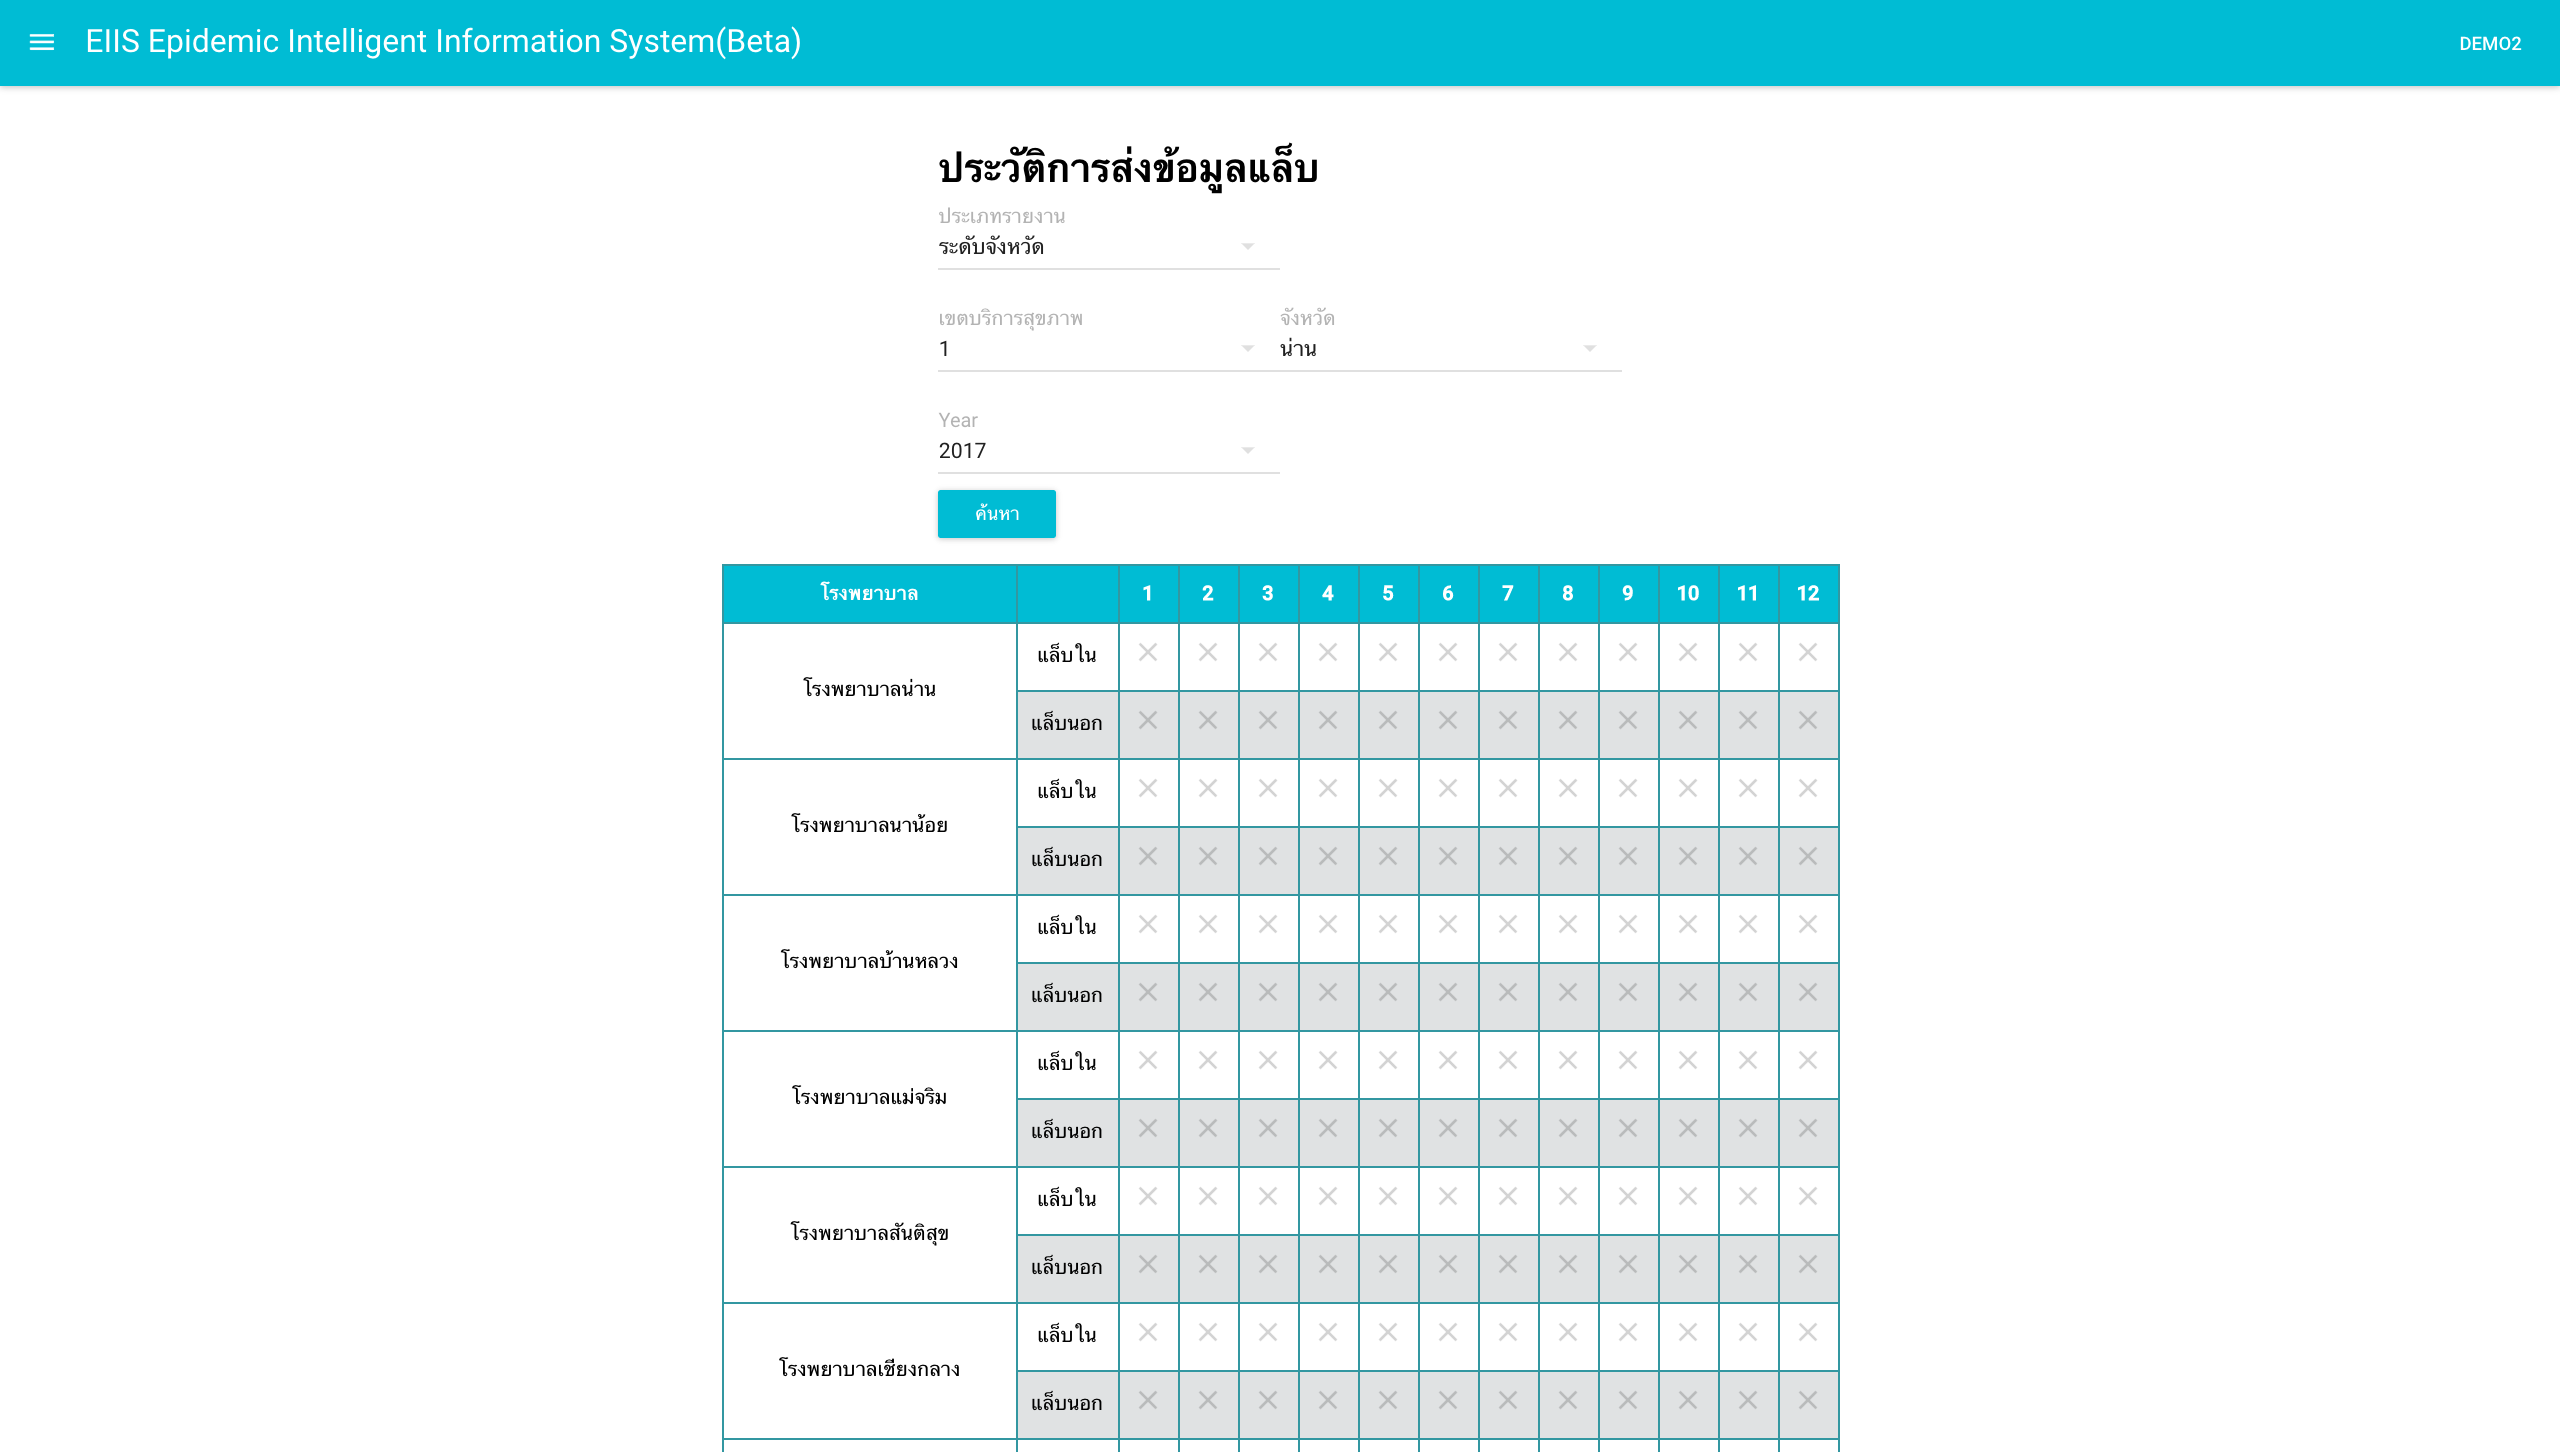
\includegraphics[width=12cm]{images/chapter-05/check-upload-status.png}
        		\caption{Status of uploaded lab files from hospitals in a region}
        		\label{upload-status}
        \end{figure}
	\FloatBarrier
	
	
	\subsection{Demographics Report} \label{demographics_report}
	
	To see at a demographics report,user need to select demographics report in tab bar menu that shown in figure \ref{tab-bar-menu}. Then, user can select type of data that they want by selecting nation, time, disease, criteria of the disease, and the type of report that they want. In order to see all the drop-down select, there are in section \ref{filter-data}. When user finished selecting, user need to click 'find' button as shown in figure \ref{demographics-report}. Then the front-end will send the input data to the server via POST. For example, /api/v1/hiv/demographic/all. Then the server will send json object back, then many type of graphs will be rendered as shown in section \ref{chart}.
	
    \FloatBarrier
    	\begin{figure}[h!]
            \centering
                % can use width=\linewidth
        		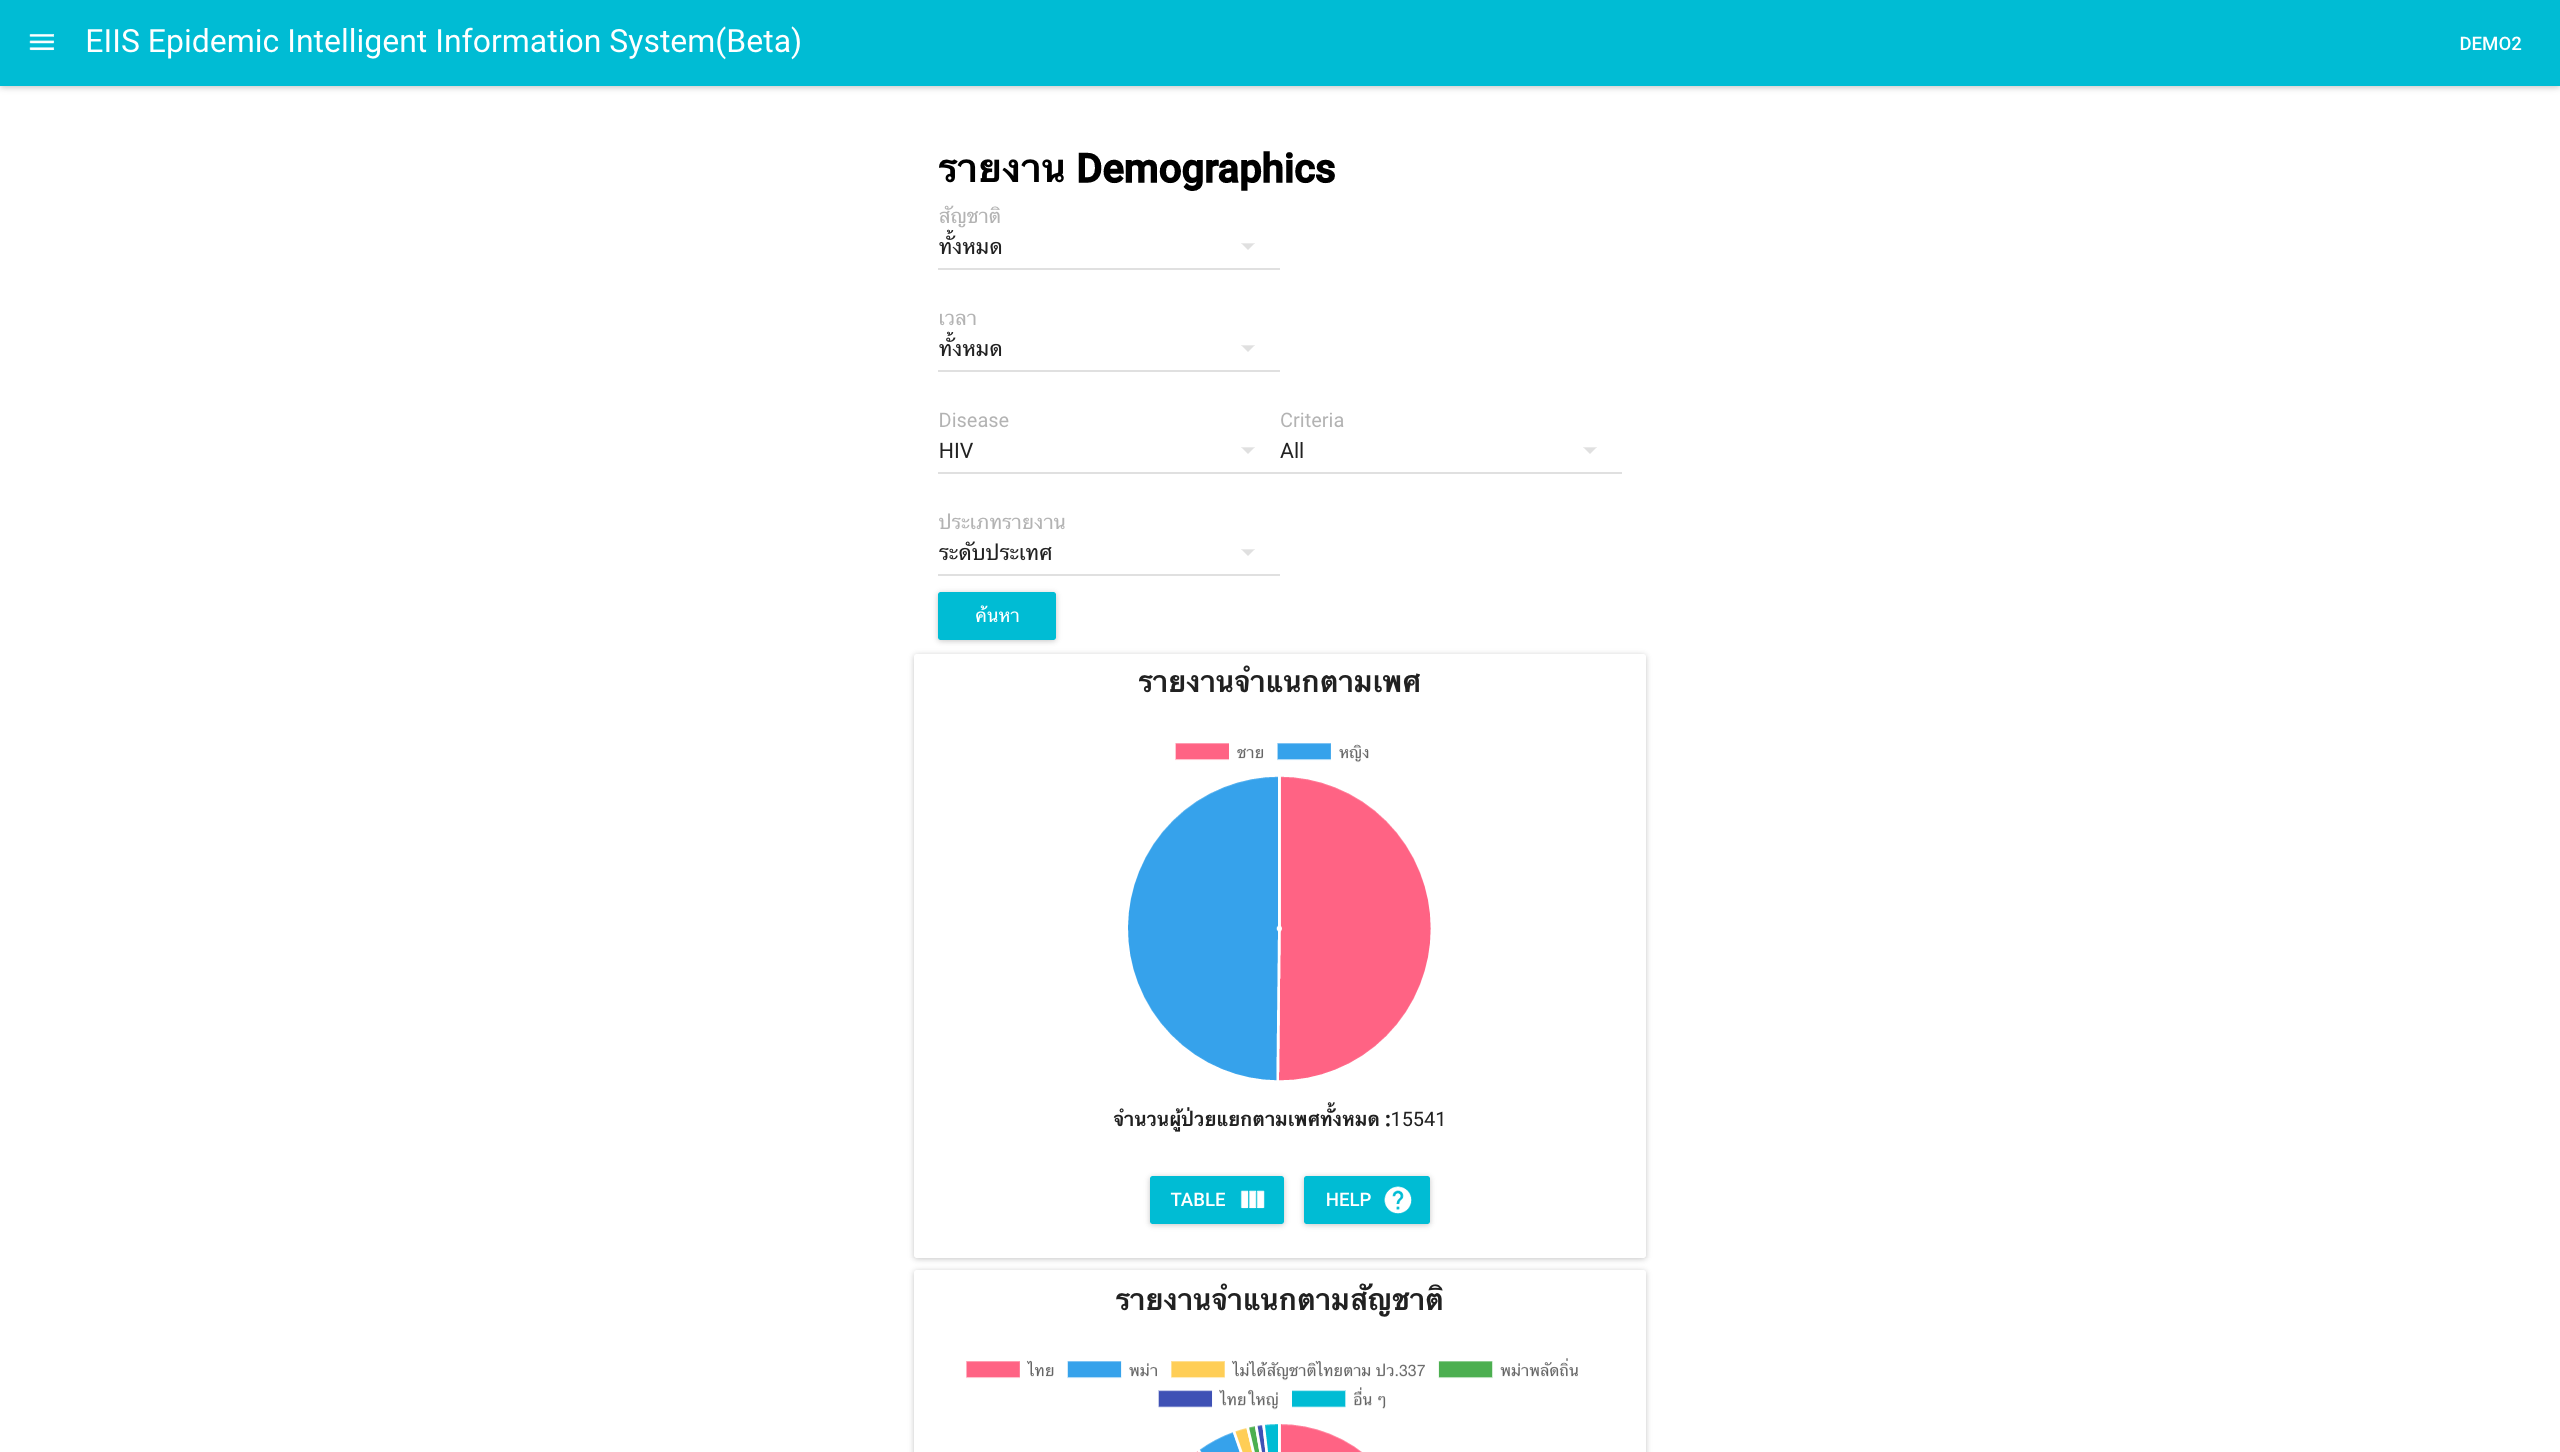
\includegraphics[width=12cm]{images/chapter-05/demographics-report.png}
        		\caption{Demographics Report}
        		\label{demographics-report}
        \end{figure}
	\FloatBarrier
	
	\subsection{Charts} \label{chart}
	   	 
	
    	\subsubsection{Pie Chart separate by Gender}
    	    In this pie chart, it shows the data between male and female. Pink means male and Blue means Women. As it shown in figure \ref{pie-graph-sex}
    	    \vspace{10mm}
        	\FloatBarrier
            	\begin{figure}[h!]
                    \centering
                        % can use width=\linewidth
                		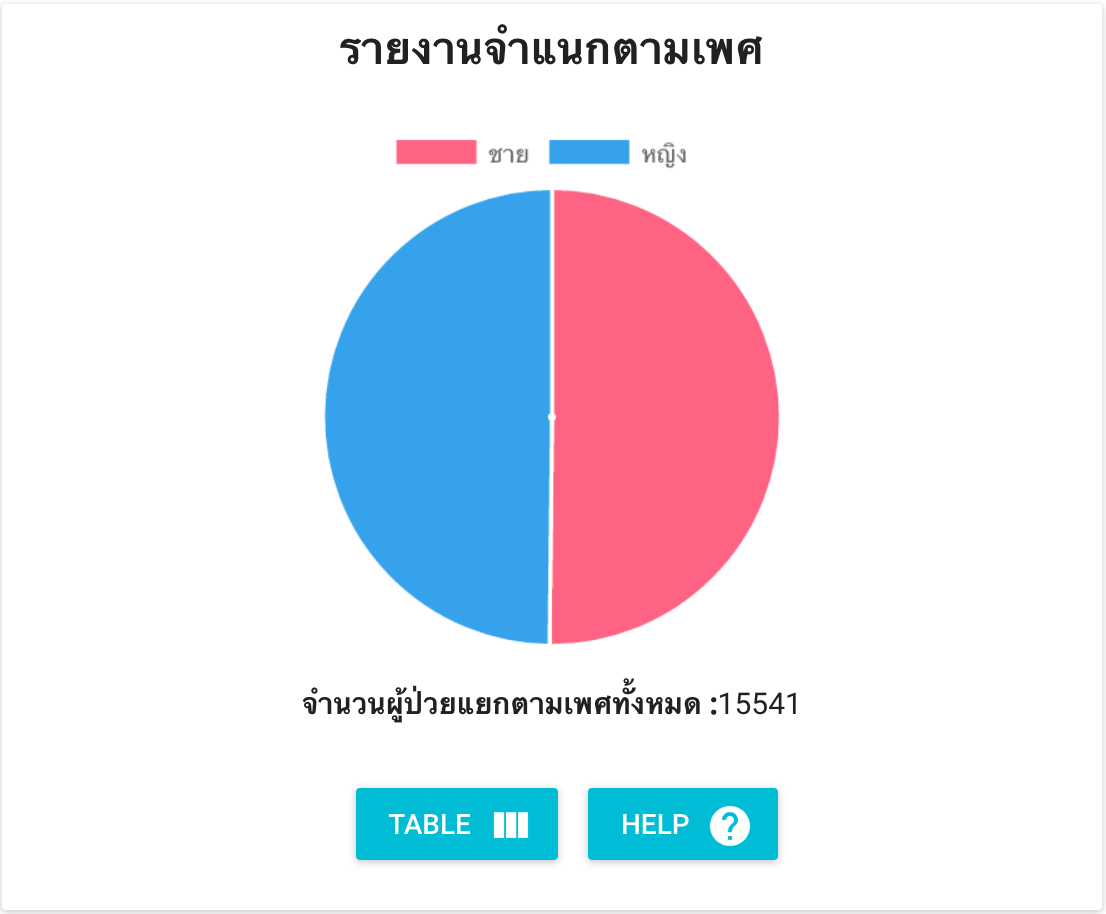
\includegraphics[width=9cm]{images/chapter-05/pie-graph-sex.png}
                		\caption{Gender Pie Chart}
                		\label{pie-graph-sex}
                \end{figure}
        	\FloatBarrier
    	\newpage
        \subsubsection{Pie Chart separate by Nation}
            In this pie chart, it shows data that separated by nation that will be sorted from the top highest. It means that it will show top five that have highest people in that nation and other group will be put in as other. As it shown in figure \ref{pie-graph-nation}
	
        	\FloatBarrier
            	\begin{figure}[h!]
                    \centering
                        % can use width=\linewidth
                		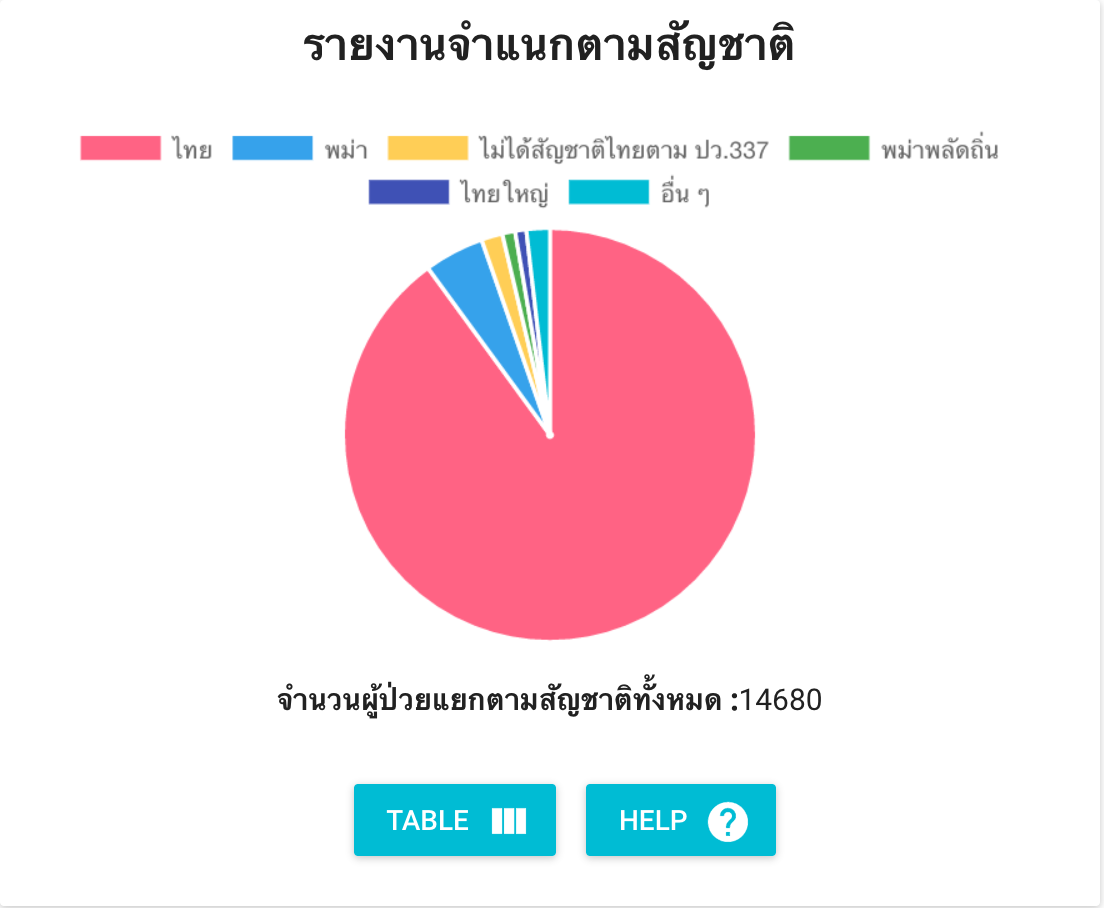
\includegraphics[width=9cm]{images/chapter-05/pie-graph-nation.png}
                		\caption{Nation Pie Chart}
                		\label{pie-graph-nation}
                \end{figure}
        	\FloatBarrier
        \subsubsection{Pie Chart separate by Occupation}
            In this pie chart, it shows data that separated by occupation that will be sorted from the top highest. It means that it will show top four that have highest people on that occupation area and other left will be put as other type. As it shown in figure \ref{pie-graph-occupation}
	
        	\FloatBarrier
            	\begin{figure}[h!]
                    \centering
                        % can use width=\linewidth
                		\includegraphics[width=8cm]{images/chapter-05/pie-graph-occupation.png}
                		\caption{Pie Chart separate by Occupation}
                		\label{pie-graph-occupation}
                \end{figure}
        	\FloatBarrier
	
	    \subsubsection{Pie Chart separate by Marital Status}
            In this pie chart, it shows data that separated by status that will be sorted from the top highest. It means that it will show top four that have highest people on that status and other left will be put as other type, as shown in figure \ref{pie-graph-status}
	
        	\FloatBarrier
            	\begin{figure}[h!]
                    \centering
                        % can use width=\linewidth
                		\includegraphics[width=9cm]{images/chapter-05/pie-graph-status.png}
                		\caption{Marital Status Pie Chart}
                		\label{pie-graph-status}
                \end{figure}
        	\FloatBarrier
	
	    \subsubsection{Histogram Separate by Gender}
            In this histogram, it shows histogram that separate data by age and gender. On the horizontal scale will tell you about age. It is ordered from less to high, and in the vertical, it shows the amount number of people. Furthermore, in this graph will compare between male and female as you can see in the graph below. Green means male and orange means female. As it shown in figure \ref{graph-age-sex}
              
    	\FloatBarrier
        	\begin{figure}[h!]
                \centering
                    % can use width=\linewidth
            		\includegraphics[width=9cm]{images/chapter-05/graph-age-sex.png}
            		\caption{Histogram separate by Gender}
            		\label{graph-age-sex}
            \end{figure}
    	\FloatBarrier
    	
    	\subsubsection{Pie Chart separate by Province}
            In this pie chart, it shows data that separated by province that will be sorted from the top highest. It means that it will show top ten that have highest people on that province area and other left will be put as other type. As it shown in figure \ref{pie-graph-province}
	
    	\FloatBarrier
        	\begin{figure}[h!]
                \centering
                    % can use width=\linewidth
            		\includegraphics[width=9cm]{images/chapter-05/pie-graph-province.png}
            		\caption{Pie Chart separate by Province}
            		\label{pie-graph-province}
            \end{figure}
    	\FloatBarrier
    	
    	\subsubsection{Pie Chart separate by Hospital}
            In this pie chart, it shows data that separated by hospital that will be sorted from the top highest. It means that it will show top five that have highest people in that hospital and other left will be put as other type. As it shown in figure \ref{pie-graph-hospital}
	
    	\FloatBarrier
        	\begin{figure}[h!]
                \centering
                    % can use width=\linewidth
            		\includegraphics[width=9cm]{images/chapter-05/pie-graph-hospital.png}
            		\caption{Pie Chart separate by Hospital}
            		\label{pie-graph-hospital}
            \end{figure}
    	\FloatBarrier
    	
    	\subsubsection{Pie Chart Between AIDS and Non-AIDS}
    % 	???????????  Aids and non-AIDs
    	   % diagnosis result (Z21,B20X,B21X)by the doctor
            In this pie chart, it shows data that separated between AIDS and Non-AIDS. AIDS means that patient who have the diagnosis result from ICD-10 ( International Statistical Classification of Diseases and Related Health Problems) which are "B20", "B21" and "B22". Non-AIDS means that patient who do not have a lab result. Blue means AIDS and pink means Non-AIDS As the chart shown in figure \ref{pie-graph-seperate-disease}. However, this graph is shown only when user choose HIV in disease drop-down.

    	\FloatBarrier
        	\begin{figure}[h!]
                \centering
                    % can use width=\linewidth
            		\includegraphics[width=9cm]{images/chapter-05/pie-graph-seperate-disease.png}
            		\caption{Pie Chart Between AIDS and Non-AIDS}
            		\label{pie-graph-seperate-disease}
            \end{figure}
    	\FloatBarrier
	
	
	    \subsubsection{Pie Chart Separate by Medication}
	    
	        This pie chart will show when user select HIV in the disease drop-down. In this pie chart, it shows data that separated by drug. Active drug means patient who have HIV that still get the drug, and inactive drug means patient who have HIV that not get the drug
	        Blue means inactive drug and pink means active drug As the chart shown in figure \ref{pie-graph-receive-medicine}. However, this graph is shown only when user choose HIV in disease drop-down.
	        
           
        	\FloatBarrier
            	\begin{figure}[h!]
                    \centering
                        % can use width=\linewidth
                		\includegraphics[width=9cm]{images/chapter-05/pie-graph-receive-medicine.png}
                		\caption{Pie Chart Separate by Receiving Drug}
                		\label{pie-graph-receive-medicine}
                \end{figure}
        	\FloatBarrier
	
	
        \subsubsection{Pie Chart Separate by HIV and TB}
        
        	This pie chart is very special because it is the only place that can show pie chart that separate by HIV and TB. The reason that it is very special is because the data(43 folder), that we received, can analysis and show the pie chart that can count people who have HIV and TB at the same time. This pie chart shows data that separated by TB and Non-TB. TB here means patient who have HIV and also have TB as represented in blue and Non-TB means patient who have HIV but do not have TB as represented in pink. As the pie chart is shown in figure \ref{pie-graph-hiv-tb}. However, this graph is shown only when user choose HIV in disease drop-down.
    	
    	\FloatBarrier
        	\begin{figure}[h!]
                \centering
                    % can use width=\linewidth
            		\includegraphics[width=9cm]{images/chapter-05/pie-graph-hiv-tb.png}
            		\caption{HIV TB Pie Chart}
            		\label{pie-graph-hiv-tb}
            \end{figure}
    	\FloatBarrier
    	
    	\subsubsection{HIV Follow Up Chart}
    	
    	In this bar chart, it will show HIV follow up, the purpose of this graph is to follow the patient who have HIV. There are five main bar in this chart which are patient who have HIV, on ARV, last visit(in a year), viral load in a year, and viral suppressed. In the horizontal scale, there will be the topics and the vertical scale will be the amount of people. the first bar means people who have HIV, so it will count the people who have HIV. The second bar (on ARV) means people who have to get Antiretroviral drugs. The third bar means patient who last visit to hospital in the a year. the fourth bar(viral load in a year) means patient who go to check viral load in a year which patient can go check at hospital. The last bar(viral suppressed) means patient who go to check viral load in a year and the value is low.

	
    	\FloatBarrier
        	\begin{figure}[h!]
                \centering
                    % can use width=\linewidth
            		\includegraphics[width=9cm]{images/chapter-05/pie-graph-follow-hiv.png}
            		\caption{HIV Follow Up Chart}
            		\label{pie-graph-follow-hiv}
            \end{figure}
    	\FloatBarrier
	
% 	\subsection{Individual Report}
	
	\subsection{Log-Out}
	
	
	To log-out, user need to select log-out in tab bar menu that shown in figure \ref{log-out}.  After that the front-end will use POST method as /api/v1/auth/logout in order to log-out. After that it will bring you to the log-in page as shown in figure \ref{log-in}.
	
	\vspace{10mm}
    \FloatBarrier
    	\begin{figure}[h!]
            \centering
                % can use width=\linewidth
        		\includegraphics[width=10cm]{images/chapter-05/log-out.png}
        		\caption{Log-Out}
        		\label{log-out}
        \end{figure}
	\FloatBarrier
    \chapter{Backend Implementation}

    \section{Architecture Overview}
        % Migrating from Express + MongoDB
        % Reasons: MapReduce in MongoDB has price of speed performance
        Before we choose Scalatra to be the server side of the system, we had been using Express\cite{expressjs} for the server and MongoDB\cite{mongodb} for the database. However, the reason why we migrate from this stack into Scalatra\cite{scalatra} is due to the performance of MapReduce in MongoDB. We use mapReduce database command for counting the number of people who has HIV, AIDS, TB, and STD disease in each case according to the requirements. MapReduce does not guarantee the speed of computation. It is not supposed to be used in the real time application. Moreover, as our system will contain more data, the speed performance will most likely to be dropped. This is the reason why we moved from Express and MongoDB stack into Scalatra for the backend.
        
    \section{Data Preprocessing}
    
        % ICT update data every 15 days via rsync command
        % It took a whole day since size of data is huge (1 TB)
        % contain irrelevant information (non-related visits)
        % 946 GB (from 2014 to now), Person: 421,444,580, Diagnosis: 1,423,970,811 record
        
        As we mentioned earlier in chapter \ref{section:how-the-data-flow} of how the data flow. First, ICT will update the data which is all the records of 43 health folders to our server in every 15 days by using rsync command. However, the process takes a whole day since the size of the data is 946 GB (since 2014 until 30 March 2017) which almost 1 TB. It contains 421,444,580 people and 1,423,970,811 diagnosis record which are include irrelevant information about the visits that do not have diseases under surveillance such as patient received paracetamol, vitamin C and etc. Within this size of data, our server will not be able to process all the data in reasonable duration of time. Therefore, we need to do multiple steps of data preprocessing before our data is ready for production.
        
        Let begin with when our server receive the data we need to create indexing to filtering our relevant 43 folder such as PERSON, LABFU, DIAGNOSIS{\_}IPD, DIAGNOSIS{\_}OPD, DRUG{\_}IPD, and DRUG{\_}OPD etc. Those indexing file create under the condition that those record are possible to relate to disease under surveillance. There are 4 indexing file that we create. First file is hp file where it store the hospcode and PID. Second file name hpa contain hospcode, PID and AN (admission number). Third file is hps which contain hospcode, PID, and SEQ. Last file is hn which contain hospcode and HN for our extra lab file because some lab file that upload to our system are not contain PID that use to be the linker of patient and lab result. Note that in this step we already get some filter raw file include LABFU, DIAGNOSIS{\_}IPD, DIAGNOSIS{\_}OPD, DRUG{\_}IPD, and DRUG{\_}OPD.
        
        After we create indexing file, now we go in to the process of filtering where the size of data will going to be reduce. We filter all relevant 43 folder using the most appropriate indexing file we create in the previous step. First we use hp file to filter PERSON, DEATH, ADDRESS and PRENATAL folder. We use hpa file to filter ADMISSION folder and use hps to filter SERVICE folder to delete all unrelate case such as broken leg, headache and etc. We use hn file to link the patient and extra lab result together.
        In addition, doing the process of filtering out some data we also anonymize all the sensitive information including hash all CID (Citizen identification number), change birth date to the first day of the month like 25 June 1956 to become 1 June 1956 because we only need to age of the patient and remove all first name, last name and etc. At the end of this process the data size will reduce very much for exmple in PERSON folder from approximate 400 million people to around 1 million people.
        
        Next, we need to perform indexing the data by hash cid. Before this step, all the data is grouped by province. However, if we group the data by province, it will be way more difficult to follow up the patient how many hospitals he/she visit in time series. Therefore, we need to perform indexing every record of the data by hash cid. First, we create a large hashmap by using hospcode and pid as the key to look for hash cid in PERSON folder. After that, we put the hash cid as the first column in every health folders that we use. We also perform sorting the data by hash cid.

        To make our backend system be able to perform parallel processing task when receive such request, we create a virtual shard. First, we set a number of shards to be 256. Then, we iterate through each record of each person. Next, we check if the hash cid of that person modulo with number of shard (in this case, 256) equals to zero. If it is, we put the record of that person into that shard. By doing this, it will always guarantee that every record that belongs to one person will belong to exactly 1 shard. There will be no record of that person goes across the shard. By doing this, it will give us benefit of parallel processing.
        
        \FloatBarrier
            \begin{figure}[h!]
                \centering
                    % can use width=\linewidth
                	\includegraphics[width=\linewidth]{images/chapter-06/data_reduction.png}
                	\caption{Data Preprocessing Diagram}
                	\label{data_preprocessing}
            \end{figure}
        \FloatBarrier
    
    \section{Implementation}
    
        % \subsection{Skimming Data}
        %     Originally, all the data from 43 folders that we got from Information Technology and Communication Center (under Office of the Permanent Secretary, Ministry of Public Health) since 2014 has the size of the data  more than 900 Gigabytes. It includes all the cases that patient visit to the hospital such as broken leg, headache, HIV, etc. Hence, every cases except HIV, AIDS, TB, and STD is irrelevant to our system.
            
        %     We filtered out the data that is not related to our system, hashing the citizen id number (protecting the privacy of the person), and group the remaining data by the hash result. We also sorted the data by the hash result. Hence, the size of the data is reduced into less than four Gigabytes.
        %     % separate file and hash (group & sort)
        % \subsection{Filter Data From Client Request} \label{filter-data}
        %     First of all before we go through on how server side work, we will explain how each drop-down select works. There are four main type of drop-down select as shown below.
        %     \subsubsection{Nation Drop-Down}
    In the nation drop-down button as shown in figure \ref{figure-nation-drop-down}, if user choose one of the lists as shown in figure \ref{figure-nation-lists}, it will be sent the value to the server which that the server will pass the nation filter to match that which type that user choose. Then it will get the the code of the country such as Thailand is 099, Myanma is 048, Laso is 056, and Cambodia is 057, in order to correctly count people in each nation depending on the nation filter.
    
% Thai = 099
%   val MYANMA: String = "048"
%   val LAOS: String = "056"
%   val CAMBODIA: String = "057"

    \FloatBarrier
        \begin{figure}[h!]
            \centering
                % can use width=\linewidth
        		\includegraphics[width=\linewidth]{images/chapter-06/nation-1.png}
            	\caption{Nation Drop-Down}
        		\label{figure-nation-drop-down}
        \end{figure}
    \FloatBarrier
    
    \FloatBarrier
        \begin{figure}[h!]
            \centering
                % can use width=\linewidth
        		\includegraphics[width=\linewidth]{images/chapter-06/nation-2.png}
            	\caption{Nation Lists}
        		\label{figure-nation-lists}
        \end{figure}
    \FloatBarrier
    
\subsubsection{Time Drop-Down}  

    
    In time drop-down button as shown in figure \ref{figure-time-drop-down}, there are three different type of it that user can choose as shown in figure \ref{figure-time-lists}. First, if user chooses all, it means that the server will choose time at the beginning of the data until the end of the data. The beginning here mean the first date of the data and the 23:59 of the end of the data. Second, if user chooses time-interval as shown in figure \ref{figure-time-interval-drop-down}, it means the server will choose the first date of the starting month, and follow by the month and the year that user choose to be the starting date time. Then it will end up at the end date of that month, the month and year that user choose as shown in figure \ref{figure-time-interval-drop-down}Third, if user chooses cut-off time as shown in figure  \ref{figure-time-end-date-drop-down}, it means that the server will choose the starting date at the beginning of the data and it will end up at the end date of the month that user choose, month, and year that user choose as shown in figure \ref{figure-time-end-date-drop-down}. In addition, the beginning date means that will pick the start of the date. for example if user choose first month and 2017, it means that the server will choose 1/1/2017. Unlike the beginning date, the end date will choose the last first of the date that pick, for instance, if user choose end date as second month and 2017, the server will choose 31/1/2017 at time 23:59.9.
    

    \FloatBarrier
        \begin{figure}[h!]
            \centering
                % can use width=\linewidth
        		\includegraphics[width=9cm]{images/chapter-06/time-all.png}
            	\caption{Time Drop-Down}
        		\label{figure-time-drop-down}
        \end{figure}
    \FloatBarrier
    
    \FloatBarrier
        \begin{figure}[h!]
            \centering
                % can use width=\linewidth
        		\includegraphics[width=9cm]{images/chapter-06/time-lists.png}
            	\caption{Time Lists}
        		\label{figure-time-lists}
        \end{figure}
    \FloatBarrier
    
    \FloatBarrier
        \begin{figure}[h!]
            \centering
                % can use width=\linewidth
        		\includegraphics[width=\linewidth]{images/chapter-06/time-interval.png}
            	\caption{Time Interval Drop-Down}
        		\label{figure-time-interval-drop-down}
        \end{figure}
    \FloatBarrier
    
    \FloatBarrier
        \begin{figure}[h!]
            \centering
                % can use width=\linewidth
        		\includegraphics[width=\linewidth]{images/chapter-06/time-end-date.png}
            	\caption{Time End Date Drop-Down}
        		\label{figure-time-end-date-drop-down}
        \end{figure}
    \FloatBarrier
    
\subsubsection{Disease and Criteria Drop-Down}
    In disease and criteria drop-down button as shown in figure \ref{figure-disease-drop-down} and \ref{figure-disease-lists}, there are for different type of diseases that user can choose. Also in each disease there are many criteria that user can choose. It means that criteria will change according to the disease as shown in figure \ref{figure-disease-lists}. First, if user choose HIV, the criteria will show as in figure \ref{figure-disease-hiv-lists}, "All" means that choosing both HIV confirmed and HIV presumed. HIV confirmed means that patient who have diagnosis result (Z21, B20X, B21X) by the doctor and HIV presumed means that patient who receiving antiviral drug more than two types. "Confirmed" means choosing only HIV confirmed, and "HIV TB Comorbidity" means the server will choose patient that have HIV all and also the patient should have TB.
    % ?? "HIV TB" ==> which type of hiv(confirm or all)
    
    Second, if user choose Hepatitis C, the criteria will show as in figure \ref{figure-disease-hepatitis-c-lists}, "All" means choosing all patient that have diagnosis test in the criteria of hepatitis C. "Acute" means patient that has the diagnosis result of (B171, B1710, B1711) by the doctor and can be cured by the drug. "Chronic" means choosing the patient from the diagnosis result of (z2252,B182,B192,B1920,B1921) and this is the stage 2 that develop from acute if there is no drug action taken. It is when virus damages the liver enough to cause the signs and symptoms of liver disease. "Cirrhosis" means choosing the patient from the diagnosis result of (K743,K744,K745,K746) and have the previous diagnosis result in range of hepatitis C. Cirrhosis happen when the patient have permanent scar tissue replaces healthy liver cells from the virus of hepatitis C. "Hepatocellular Carcinoma" means the diagnosis result of the patient is C220 and have the previous diagnosis result in range of hepatitis C. It is a dead stage where patient need surgery as the hepatitis C virus developed to become the cancer.
    
    Third, if user choose Hepatitis B, the criteria will show as in figure \ref{figure-disease-hepatitis-d-lists}, All" means choosing all patient that have diagnosis test in the criteria of hepatitis B. "Acute" means choosing the patient that get the diagnosis result of (B160,B161,B162,B169) and can be cured by drug. "Chronic" means choosing the patient that has the diagnosis result of (Z2251,B180,B181,B191,B1910,B1911). Chronic hepatitis B is a development from acute stage of hepatitis B where there is no treatment taken place. "Acute With HDV" means the patient has the diagnosis of B160 or B161. It only happen to the patient who carry hepatitis B to be infect by HDV or Delta agent (Hepatitis D) and make the symptom of the patient get worse. "Chronic With HDV" means choosing the patient from the diagnosis result of B180 and the patient are infect to hepatitis D after carry the hepatitis B virus. "Cirrhosis" has the same diagnosis result as same as cirrhosis in hepatitis C but cause from the hepatitis B instead. "Hepatocellular Carcinoma" means choosing the patient diagnosis result of C220 and have the previous diagnosis result in the type of hepatitis B. It is the stage where the virus become cancer and patient need to surgery.
    
    Lastly, if user choose TB, There is only one criteria in this field which is "All". It means patient who have TB.
    
    
    \FloatBarrier
        \begin{figure}[h!]
            \centering
                % can use width=\linewidth
        		\includegraphics[width=9cm]{images/chapter-06/disease.png}
            	\caption{Disease Drop-Down}
        		\label{figure-disease-drop-down}
        \end{figure}
    \FloatBarrier
    
    \FloatBarrier
        \begin{figure}[h!]
            \centering
                % can use width=\linewidth
        		\includegraphics[width=9cm]{images/chapter-06/disease-lists.png}
            	\caption{Disease Lists}
        		\label{figure-disease-lists}
        \end{figure}
    \FloatBarrier
    
    \FloatBarrier
        \begin{figure}[h!]
            \centering
                % can use width=\linewidth
        		\includegraphics[width=9cm]{images/chapter-06/disease-hiv-lists.png}
            	\caption{HIV Lists}
        		\label{figure-disease-hiv-lists}
        \end{figure}
    \FloatBarrier
    
    \FloatBarrier
        \begin{figure}[h!]
            \centering
                % can use width=\linewidth
        		\includegraphics[width=9cm]{images/chapter-06/disease-hepatitis-c-lists.png}
            	\caption{Hepatitis C Lists}
        		\label{figure-disease-hepatitis-c-lists}
        \end{figure}
    \FloatBarrier
    
    \FloatBarrier
        \begin{figure}[h!]
            \centering
                % can use width=\linewidth
        		\includegraphics[width=8cm]{images/chapter-06/disease-hepatitis-d-lists.png}
            	\caption{Hepatitis B Lists}
        		\label{figure-disease-hepatitis-d-lists}
        \end{figure}
    \FloatBarrier


\subsubsection{Type of Report Dropdown}


    
    
    In type of report drop-down button as shown in figure \ref{figure-type-of-report-drop-down}, there are four different type of it that user can choose as shown in figure \ref{figure-type-of-report-lists}. First, if user chooses "Country", it means that the server will select all hospitals. Second, if user chooses "Area", it will pop-up area drop-down as shown in figure \ref{figure-type-of-report-area}, it means that the server will select the data according to the area that user choose. Third, if user chooses "Province" it will pop-up area drop-down and province drop-down  as shown in figure \ref{figure-type-of-report-province}, it means that the server will choose the data according to the province that user choose. Before user choose the province, the list of the province will be picked from the area that user choose. Lastly, if user chooses "Hospital" it will pop-up area drop-down, province drop-down, and hospital drop-down  as shown in figure \ref{figure-type-of-report-hospital}, it means that the server will choose the data according to the hospital that user choose. Like choosing "Province", the list of hospital will be picked from the province that user choose and the list of province will be picked according to the area that user choose.

    

    \FloatBarrier
        \begin{figure}[h!]
            \centering
                % can use width=\linewidth
        		\includegraphics[width=9cm]{images/chapter-06/type-of-report-all.png}
            	\caption{Type of Report Drop-Down}
        		\label{figure-type-of-report-drop-down}
        \end{figure}
    \FloatBarrier
    
    \FloatBarrier
        \begin{figure}[h!]
            \centering
                % can use width=\linewidth
        		\includegraphics[width=9cm]{images/chapter-06/type-of-report-lists.png}
            	\caption{Type of Report Lists}
        		\label{figure-type-of-report-lists}
        \end{figure}
    \FloatBarrier
    
    \FloatBarrier
        \begin{figure}[h!]
            \centering
                % can use width=\linewidth
        		\includegraphics[width=\linewidth]{images/chapter-06/type-of-report-area.png}
            	\caption{Type of Report (Area Drop-Down)}
        		\label{figure-type-of-report-area}
        \end{figure}
    \FloatBarrier
    
    \FloatBarrier
        \begin{figure}[h!]
            \centering
                % can use width=\linewidth
        		\includegraphics[width=\linewidth]{images/chapter-06/type-of-report-province.png}
            	\caption{Type of Report (Province Drop-Down)}
        		\label{figure-type-of-report-province}
        \end{figure}
    \FloatBarrier
    
    \FloatBarrier
        \begin{figure}[h!]
            \centering
                % can use width=\linewidth
        		\includegraphics[width=\linewidth]{images/chapter-06/type-of-report-hospital.png}
            	\caption{Type of Report (Hospital Drop-Down)}
        		\label{figure-type-of-report-hospital}
        \end{figure}
    \FloatBarrier




    
        \subsection{At a Glance Report}\label{at_a_glance_report_back_end}
            As we know that we use POST method(for example, api/v1/hiv/at-a-glance/all) and pass it with body which contain all choose value that user choose in \ref{filter-data} then pass to the server. In server side, first it will filter by taking all the choose value to filter in order to make a correct structure and continue to do a map-reduce. After that it will return the json data to front-end.
            
            % all choose ==> filter ==> mapreduce ==> Json
        
        \subsection{Upload Lab File} \label{upload_file_back_end}
            % Only UPLOADER can upload lab file to the system
            The backend ensures that the user must have permission for uploading lab file into the server which mean the user must have "UPLOADER" role. Otherwise, it will reject by sending HTTP 401 status code (unauthorized). After the user uploaded the lab file, the server will response with total number of lines from the lab file, number of lines with correct format, number of lines with wrong format, and the lines with wrong format.
        
        \subsection{Checking Upload Lab File History Status }         \label{check_upload_history_status_ui_back_end}
            For this feature, every roles of the user can view the status of the uploaded lab files whether it has been uploaded or not during the selected year that user selected. When the user send the request, the server will return every hospitals within the province from the request and mark both in-patient lab file and out-patient lab file with boolean status whether that lab file has been uploaded to the system or not.
            
        
        \subsection{Demographics Report} \label{demographics_report_back_end}
            
            As we know that we use POST method(for example, /api/v1/hiv/demographic/all) and pass it with body which contain all choose value that user choose in \ref{filter-data} then pass to the server. In server side, first it will filter take all the choose value to filter in order to make a correct structure to continue to do a map-reduce. After that it will return the json data to front-end.
        % all choose ==> filter ==> mapreduce ==> Json
            
            
        % \subsection{Workload Report} \label{workload_report_backend}
        
        % \subsection{Individual Report}\label{individual_report_back_end}
        
        \subsection{Authentication}
            \subsubsection{Login}
                Authentication plays a major role in our system since the data is sensitive. We already create user accounts for all the users in our system. This means each hospital will have 1 account in our system. If the hospital's staff is changed, the account is still the same. If the user sign in successfully, we store the cookie into the browser. Otherwise, the server will return HTTP 401 status (unauthorized).
            \subsubsection{Logout}
                Once the user click logout on the web page, it will send the post request to /api/v1/auth/logout to the server. The server then will set the cookie to be expired and the user will need to login again to be able to interact with the system.
        
        
    \section{Unit Testing}
        We perform some unit testing on the backend since it defines the structural behavior of the system. There are some unit tests for API responses, authentication, model. We use ScalaTest\cite{scalatest} as our testing tool.

% multiple inheritance 


    \chapter{Deployment}

% \section{Traditional Deployment vs Application Containerization}
\section{Application Containerization}
    In this system, we use Docker\cite{docker} to containerize our application into 5 containers. There are MongoDB, Scalatra, Frontend, Version Service, and Nginx containers as shown in Figure \ref{fig:system-architecture}. There are several reasons why we choose to use Docker for deploying our application instead of deploying it in a traditional way. The first reason is the different environment between development and production. If we were to deploy our application in a traditional way, we would need to configure each of our components (MongoDB, backend, frontend, and Nginx) step by step. If our server is crashed and we need to deploy our application into the new server, we will need to redo every step from the beginning. However, when we use Docker for deployment, the different environments is no longer a problem since we can use production environment on our development machine (e.g., laptop) and then deploy it with the same configuration to our server. The  second reason why we choose Docker for deployment is that the host system does not have to depend on any dependencies of the application. As long as the host system can run Docker, it should be able to run Docker containers whereas on the traditional deployment, we would have to install all the dependencies that our application needs. The third reason is the resource utilization. Docker containers are lightweight and each container will have its own resources which are isolated from other containers. A container will not consume all the available resources of the host system in which can decrease the performance of other applications.
    
    \newpage
    \section{Containers Flow}
        When a http request comes to / with port 80, it will go to Nginx Container and the container will route it to Frontend Container. When the Frontend Container calls API service via /api, the request will first go to Nginx Container and then will be routed to Scalatra Container. Scalatra Container connects to MongoDB Container for user authentication. Finally, there is also Version Service Container which provides the version number of both frontend and backend by showing the number of commits.
        

    \FloatBarrier
    	\begin{figure}[h!]
            \centering
                % can use width=\linewidth
        		\includegraphics[width=\linewidth]{images/chapter-07/system-architecture.png}
        		\caption{Containerized Application Architecture}
        		\label{fig:system-architecture}
        \end{figure}
    \FloatBarrier
    
\section{Failure Handling}
    Failure handling in this project is convenient since we containerized our application using Docker. There are restart policies that Docker has provided. The restart policy that we are using in the system is "unless-stopped" which means it will always restart the container no matter the exit status is but it will not restart the container if the container is stopped by the user.
    \chapter{Summary}

\section{Future Works}
    \subsection{Individual and Workload Report}
        According to the change of our backend from express to scalatra, we need to reimplemented both individual report and workload report to match our requirement.
    % monitor more diseases
    \subsection{Monitoring more diseases}
        Currently, our system is designed for monitoring some of disease that are under surveillance of Ministry of Public Health, Thailand which are HIV, AIDS, TB, Hepatitis, and STD. However, we plan to scale up our system by having our system monitoring more diseases that are under surveillance of Ministry of Public Health such as Malaria, Dengue etc.
    \subsection{Automated Updating On Receiving New Data Sources}
        % bot
        % merge and indexed
        % Information Technology and Communication Center
        At the moment, when the 43 folders were sent to Information Technology and Communication Center, ICT Center already provided rsync command to update the data into the production server. Nevertheless, we have to merge and index the new data with existing data manually. We plan to implement the automated task for merging and indexing the data when there is any update of the data from ICT Center.

    \appendices{}
% This adds "Appendices" to TOC
\addappheadtotoc
\chapter{43 folder detail}
    \section{PERSON}
        \label{person_folder}
        \begin{enumerate}
  \item HOSPCODE: Hospital code that is defined by the Bureau of Policy and Strategy (under Ministry of Public Health).
  \item CID: Citizen identification number 
  \item PID: Person identification number who registers in the hospital. This is used for identifying the person in other folders (the range of digits can be between 1 to 15 and generated by program).
  \item HID: House code
  \item PRENAME: The name prefix in which comes from the standard from Department of Provincial Administration (under Ministry of Interior).
  \item NAME: Name of the person.
  \item LNAME: Last name of the person.
  \item HN: Hospital number that is used for registering patient into the record (the range of digits can be between 1 to 15 and generated by program).
  \item SEX: 1 = male, 2 = female
  \item BIRTH: Date of birth which is in YYYYMMDD format. Using CE format for the year.
  \item MSTATUS: Marital Status. 1 = Single, 2 = Married, 3 = Widowed, 4 = Divorced, 5 = Separated, 6 = Monk, 9 = Unknown
  \item OCCUPATION\_OLD: Previous code of person's occupation code that is defined by Bureau of Policy and Strategy (under Ministry of Public Health).
  \item OCCUPATION\_NEW: Current code person's occupation that is defined by Bureau of Policy and Strategy (under Ministry of Public Health).
  \item RACE: Person's race code that is defined by Department of Provincial Administration (under Ministry of Interior).
  \item NATION: Person's nationality code that is defined by Department of Provincial Administration (under Ministry of Interior). If it is unknown, mark it as 999.
  \item RELIGION: Person's religion code that is defined by Bureau of Policy and Strategy (under Ministry of Public Health).
  \item EDUCATION: Person education's level code that is defined by Bereau of Policy and Strategy (under Ministry of Public Health).
  \item FSTATUS: Family Status. 1 = Host, 2 = Tenant
  \item FATHER: The CID of person's father (in case a person's age is below 15).
  \item MOTHER: The CID of person's mother (in case a person's age is below 15).
  \item COUPLE: The CID of person's spouse.
  \item VSTATUS: Person's status in the community. 1 = Subdistrict Headman or Village Headman, 2 = Volunteer, 3 = Subdistrict Medical Practitioner, 4 = Member of the Subdistrict Administrative Organization Council, 5 = etc
  \item MOVEIN: The date that person move into region that has responsibility for him/her. The format is YYYYMMDD and the year format is CE.
  \item DISCHARGE: The status or cause of discharge. 1 = death, 2 = Move, 3 = Lost, 4 = Not Discharge. (In a case that a person who lives on different region from hospital or people who lives in the region that not discharge, it will be marked as 9).
  \item DDISCHARGE: The date of discharge in which the format is YYYYMMDD and the year format is CE. It will be record only when DISCHARGE is marked as 1, 2, or 3.
  \item ABOGROUP: The blood type of person. 1 = A, 2 = B, 3 = AB, 4 = O, 9 = Unknown.
  \item RHGROUP: RH blood type. 1 = positive, 2 = negative.
  \item LABOR: The foreigner code which is defined by Bureau of Policy and Strategy (under Ministry of Public Health). It will be recorded in a case that a patient is a foreigner.
  \item PASSPORT: Passport Identification Number. It will be recorded in a case that foreigner person has a passport.
  \item TYPEAREA: Status of a person. 1 = have name in household registration that in the service place and live there. 2 = have name in household registration that in the service place and not live there. 3 = live in service area but household registration is in outside service area. 4 = both household registration and living area are outside the service area. 5 = live in the service area but it isn't the same as the household registration that in the service area such as homeless. Note that foreigner who live in the service area can be record as 3, if foreigner live outside service area can be record as 4, lastly foreigner who has the name in household registration can be record as 1.
  \item D\_UPDATE: The date in which this folder has been modified. The format is YYYYMMDDHHMMSS and the year format is CE.
\end{enumerate}
        
    \section{ADDRESS}
        \label{address_folder}
        % http://www.dailyenglish.in.th/english-address/
\begin{enumerate}
  \item HOSPCODE: Hospital code that is defined by the Bureau of Policy and Strategy (under Ministry of Public Health). 
  \item PID: Person identification number who registers in the hospital. This is used for identifying the person in other folders (the range of digits can be between 1 to 15 and generated by program).
  \item ADDRESSTYPE: Type of address. 1 = Address in household registration, 2 = Address that is reachable by contact.
  \item HOUSE\_ID: House identification number that is assigned by Department of Provincial Administration (under Ministry of Interior).
  \item HOUSE\_TYPE: The type of residence. 1 = Detached House or Semi Detached House, 2 = Townhouse, 3 = Condominium, 4 = Apartment or Dormitory, 5 = Labor Home-stay, 8 = etc, 9 = unknown.
  \item ROOMNO: The room number if HOUSE\_TYPE is an apartment or dormitory.
  \item CONDO: The name of building, condominium, or dormitory.
  \item HOUSENO: Street number
  \item SOISUB: Sub lane
  \item SOIMAIN: Lane
  \item ROAD: The road's name
  \item VILLANAME: The village's name
  \item VILLAGE: The village number. Use 99 if unknown.
  \item TAMBON: Sub district code that is defined by Department of Provincial (under Ministry of Interior). Use 99 if unknown.
  \item AMPUR: District code that is defined by Department of Provincial (under Ministry of Interior). Use 99 if unknown.
  \item CHANGWAT: Province code that is defined by Department of Provincial (under Ministry of Interior). Use 99 if unknown.
  \item TELEPHONE: Telephone number
  \item MOBILE: Mobile phone number
  \item D\_UPDATE: The date in which this folder has been modified. The format is YYYYMMDDHHMMSS and the year format is CE.
\end{enumerate}
        
    \section{DEATH}
        \label{death_folder}
        \begin{enumerate}
  \item HOSPCODE: Hospital code that is defined by the Bureau of Policy and Strategy (under Ministry of Public Health). 
  \item PID: Person identification number who registers in the hospital. This is used for identifying the person in other folders (the range of digits can be between 1 to 15 and generated by program).
  \item HOSPDEATH: Hospital code in a case that patient died in the hospital. If they can not determine which hospital, mark it as 00000.
  \item AN: Inpatient number in which the patient died in the hospital
  \item SEQ: The order of the service that be provided by the program. the number is unique, and sort by order of SEQ in each service (visit).
  \item DDEATH: Date that patient died. The format is YYYYMMDD and the year format is CE.
  \item CDEATH\_A: Disease code A according to Certificate of Death. 
  \item CDEATH\_B: Disease code B according to Certificate of Death.
  \item CDEATH\_C: Disease code C according to Certificate of Death.
  \item CDEATH\_D: Disease code D according to Certificate of Death.
  \item ODISEASE: Other disease code or other factor of death according to Certificate of Death.
  \item CDEATH: Cause of death according to the Certificate of Death.
  \item PREGDEATH: 1 = Death in pregnancy, 2 = Maternal Death
  \item PDEATH: The place where patient died. 1 = In hospital, 2 = Outside hospital.
  \item PROVIDER: Doctor of patient number that is generated by the program. It must be unique within the same hospital.
  \item D\_UPDATE: The date in which this folder has been modified. The format is YYYYMMDDHHMMSS and the year format is CE.
\end{enumerate}
        
    \section{SERVICE}
        \label{service_folder}
        \begin{enumerate}
  \item HOSPCODE: Hospital code that is defined by the Bureau of Policy and Strategy (under Ministry of Public Health). 
  \item PID: Person identification number who registers in the hospital. This is used for identifying the person in other folders (the range of digits can be between 1 to 15 and generated by program).
  \item HN: Outpatient number that receive when the patient come to receive the service (the range of digits can be between 1 to 15)
  \item SEQ: The order of the service that be provided by the program. the number is unique, and sort by order of SEQ in each service (visit).
  \item DATE\_SERV: The date receiving the service. Defining format as year (in CE format), month and date  by order(YYYYMMDD). NOTE that in case have to record previous data, have to change the date to the date that receive the service.
  \item TIME\_SERV: Time hospital provide a service and defining format as  hour, minute, and second as (HHMMSS)  
  \item LOCATION: The area of the patient. There are two type of it which are (1) means area of responsibility and (2) means area of irresponsibility
  \item INTIME: The time that patient come and receive the service. There are two type of it which are (1) means in office hours and (2) means out of the office hours.
  \item INSTYPE: The right to medical care code that the patient use each visit.
%   ประเภทสิทธิการรักษา
%   รหัสสิทธิมาตรฐาน ที่ใชในการมารับบริการ
  \item INSID: The id number of the card of the right to medical care according to the type of the right to medical care.
%   หมายเลขของบัตร ตามประเภทสิทธิการรักษา
  \item MAIN: The standard code that come from Bureau of Policy and Strategy in order to describe the main service place.
  \item TYPEIN: It is a types of service that patient come to receive the service. There are four main types which are (1) means the patient come to receive the service by themselves, (2) means the patient come to receive the service according to the appointment, (3) means the patient that be transferred from one to other hospital, and (4) means the patient that be transferred from EMS.
  \item REFERINHOSP: The code of the hospital that send the patient to here. 
  \item CAUSEIN: The reason that transfer the patient to receive the service here. There are five main types which are (1) means to diagnose and treat, (2) means to diagnose, (3) means to treat and recover, (4) means to receive the service that close to their home, and (5) means to receive the service according to the patient's need.
  \item CHIEFCOMP: The important symptoms that patient has to come to use the service.
  \item SERVPLACE: The place that receive the service. There are 2 types which are (1) means in the service place and (2) means outside the service place
  \item BTEMP: The body temperature that measure when the patient come in. It should be in Celsius with two digits and one decimal place.
  \item SBP: Systolic pressure that first given. It should be three or less than three digits. Note that if cannot measure, not need to record
  \item DBP: Diastolic pressure that first given. It should be three or less than three digits. Note that if cannot measure, not need to record
  \item PR: Heart rate per minute. It should be three or less than three digits.
  \item RP: Breath rate per minute. It should be three or less than three digits.
  \item TYPEOUT: The status of patient after they are done receiving the service. There are nine main types which are (1) means receive drug and can go back home, (2) means receiving as Inpatient, (3) means the patient is sent to other hospital, (4) mean dead, (5) means dead before receiving the service at hospital, (6) means dead during the transfer process to other hospital, (7) means decline to treat. (8) means escape. (9) mean receive the service without diagnosis result.
  \item REFEROUTHOSP: The hospital code that transfer the patient to have a treatment.
  \item CAUSEOUT: The reason to transfer the patient to receive the service. There are five main types which are (1) means to diagnose and treat, (2) means to diagnose, (3) means to treat and recover, (4) means to receive the service that close to their home, and (5) means to receive the service according to the patient's need.
  \item COST: Total cost of treatment including drug, medical supplies, treatment. It should be eight digits and two decimal place. If it is no price, put 0.00.
  \item PRICE:Total price of treatment including drug, medical supplies, treatment. It should be eight digits and two decimal place. If it is no price, put 0.00.
  \item PAYPRICE: Total price that patient have to pay since it is the expenses that cannot be issued to the government. . It should be eight digits and two decimal place. If it is no price, put 0.00.
  \item ACTUALPAY: Total price that the patient have to pay. It should be eight digits and two decimal place. If it is no price, put 0.00.
  \item D\_UPDATE: The date in which this folder has been modified. The format is YYYYMMDDHHMMSS and the year format is CE.
  
  
\end{enumerate}
        
    \section{DIAGNOSIS\_OPD}
        \label{diagnosis_opd_folder}
        \begin{enumerate}
  \item HOSPCODE: Hospital code that is defined by the Bureau of Policy and Strategy (under Ministry of Public Health). 
  \item PID: Person identification number who registers in the hospital. This is used for identifying the person in other folders (the range of digits can be between 1 to 15 and generated by program).
  \item SEQ: The order of the service that be provided by the program. the number is unique, and sort by order of SEQ in each service (visit).
  \item DATE\_SERV: The date receiving the service. Defining format as year(Anno Domini(AD)), month and date  by order(YYYYMMDD). NOTE that in case have to record previous data, have to change the date to the date that receive the service.
  \item DIAGTYPE: Type of diagnosis. 1 = Principle DX, 2 = Co-Morbidity, 3 = Complication, 4 = other, 5 = External Cause, 6 = Additional Code, 7 = Morphology Code. In case of out-patient, use only 1, 4, 5 or 7.
  \item DIAGCODE: Disease code in ICD-10-TM
  \item CLINIC: Ward code that is defined by the Bureau of Policy and Strategy (under Ministry of Public Health).
  \item PROVIDER: Doctor of patient number that is generated by the program. It must be unique within the same hospital.
  \item D\_UPDATE: The date in which this folder has been modified. The format is YYYYMMDDHHMMSS and the year format is CE.
\end{enumerate}
        
    \section{DRUG\_OPD}
        \label{drug_opd_folder}
        \begin{enumerate}
  \item HOSPCODE: Hospital code that is defined by the Bureau of Policy and Strategy (under Ministry of Public Health). 
  \item PID: Person identification number who registers in the hospital. This is used for identifying the person in other folders (the range of digits can be between 1 to 15 and generated by program).
  \item SEQ: The order of the service that be provided by the program. the number is unique, and sort by order of SEQ in each service (visit). 
  \item DATE\_SERV: The date that receive the service Defining format as year(format CE), month and date by order (YYYYMMDD). NOTE that in case have to record previous data, have to change the date to the date that receive the service.
  \item CLINIC: Service department code according to Bureau of Policy and Strategy
  \item DIDSTD: The standard medicine code that is set in 24 digits and the medicine code of hospital in case that they do not have The standard medicine code.
  \item DNAME: Name of the drug
  \item AMOUNT: The amount of medicine that be provided and it has to be in 12 digit(no more than 12 digits)
  \item UNIT: Unit of medicine. It is the standard code that come from Bureau of Policy and Strategy  
  \item UNIT\_PACKING: Packing size per unit that is counting in Field UNIT  
  \item DRUGPRICE: The price of medicine that sell to the patient
  \item DRUGCOST: The buying price or the price of medicine that be received from hospital  
  \item PROVIDER: Service person number that generated from the program and the number is unique in each hospital.
  \item D\_UPDATE: The date in which this folder has been modified. The format is YYYYMMDDHHMMSS and the year format is CE.
\end{enumerate}











        
    \section{LABFU}
        \label{labfu_folder}
        \begin{enumerate}
  \item HOSPCODE: Hospital code that is defined by the Bureau of Policy and Strategy (under Ministry of Public Health). 
  \item PID: Person identification number who registers in the hospital. This is used for identifying the person in other folders (the range of digits can be between 1 to 15 and generated by program).
  \item SEQ: The order of the service that be provided by the program. the number is unique, and sort by order of SEQ in each service (visit). 
  \item DATE\_SERV: The date receiving the service. Defining format as year(format CE), month and date by order (YYYYMMDD). NOTE that in case have to record previous data, have to change the date to the date that receive the service.
%   Do we need to include ICD-10-TM??
  \item LABTEST: ICD-10-TM Laboratory Test Code
  \item LABRESULT: Results of laboratory tests (2-digit decimal point)
  \item D\_UPDATE:  The date in which this folder has been modified. The format is YYYYMMDDHHMMSS and the year format is CE.
\end{enumerate}

    \section{ADMISSION}
        \label{admission_folder}
        \begin{enumerate}
  \item HOSPCODE: Hospital code that is defined by the Bureau of Policy and Strategy (under Ministry of Public Health). 
  \item PID: Person identification number who registers in the hospital. This is used for identifying the person in other folders (the range of digits can be between 1 to 15 and generated by program).
  \item SEQ: The order of the service that be provided by the program. the number is unique, and sort by order of SEQ in each service (visit).
  \item AN: Inpatient number
  \item DATETIME\_ADMIT: Date in which the hospital admits the patient. The format is YYYYMMDDHHMMSS and the year format is CE.
  \item WARDADMIT: The ward code that admits the patients that is defined by the Bureau of Policy and Strategy (under Ministry of Public Health).
  \item INSTYPE: The right to medical care code that the patient use each visit.
  \item TYPEIN: It is a types of service that patient come to receive the service. There are four main types which are (1) means the patient come to receive the service by themselves, (2) means the patient come to receive the service according to the appointment, (3) means the patient that be transferred from one to other hospital, and (4) means the patient that be transferred from EMS.
  \item REFERINHOSP: Hospital code that refers the patient.
  \item CAUSEIN: The reason that transfer the patient to receive the service here. There are five main types which are (1) means to diagnose and treat, (2) means to diagnose, (3) means to treat and recover, (4) means to receive the service that close to their home, and (5) means to receive the service according to the patient's need.
  \item ADMITWEIGHT: Patient's kilogram weight with 1 decimal.
  \item ADMITHEIGHT: Patient's centimeter height.
  \item DATETIME\_DISCH: Date and time that the hospital discharges the patient. The format is YYYYMMDDHHMMSS and the year format is CE.
  \item WARDDISCH: The ward code that discharges the patients. The code is defined by the Bureau of Policy and Strategy (under Ministry of Public Health).
  \item DISCHSTATUS: The discharge status of the patient.
  \item DISCHTYPE: The discharge type of patient.
  \item REFEROUTHOSP: The hospital code that transfer the patient to have a treatment.
  \item CAUSEOUT: The reason to transfer the patient to receive the service. There are five main types which are (1) means to diagnose and treat, (2) means to diagnose, (3) means to treat and recover, (4) means to receive the service that close to their home, and (5) means to receive the service according to the patient's need.
  \item COST: The cost of the service with 2 decimals which include medicine, medical supplies, and medical service.
  \item PRICE: The price of the service with 2 decimals which include, medicine, medical supplies, and medical service.
  \item PAYPRICE: The price with 2 decimals that patient needs to pay since it is the expenses that can not be issued to the government.
  \item ACTUALPAY: The actual price that the patient pays.
  \item PROVIDER: Doctor of patient number that is generated by the program. It must be unique within the same hospital.
  \item D\_UPDATE: The date in which this folder has been modified. The format is YYYYMMDDHHMMSS and the year format is CE.
  \item DRG: DRG group which comes from the patient's information by Grouper program according to the Government Gazette. It has 5 digits.
  \item RW: The relative weight of the in-patient. It comes from calculation of Grouper program according to the Government Gazette. It contains 4 decimals and the digits can not be more than 6. If it is unknown, mark it as 0.0000
  \item ADJRW: The relative weight that has been adjusted.
  \item ERROR: Error code about in-patient information. It comes from calculation of Grouper program according to Government Gazette.
  \item WARNING: Warning code about in-patient information. It comes from the calculation of Grouper program according to Government Gazette.
  \item ACTLOS: Patient's amount of sleep in hospital in which the value comes from the calculation of Grouper program according to the Government Gazette.
  \item GROUPER\_VERSION: The version number of Grouper program.
\end{enumerate}

    \section{DIAGNOSIS\_IPD}
        \label{diagnosis_ipd_folder}
        \begin{enumerate}
  \item HOSPCODE: Hospital code that is defined by the Bureau of Policy and Strategy (under Ministry of Public Health). 
  \item PID: Person identification number who registers in the hospital. This is used for identifying the person in other folders (the range of digits can be between 1 to 15 and generated by program).
  \item AN: Inpatient number
  \item DATETIME\_ADMIT: Date in which the hospital admits the patient. The format is YYYYMMDDHHMMSS and the year format is CE.
  \item WARDDIAG: The ward code that admits the patients that is defined by the Bureau of Policy and Strategy (under Ministry of Public Health).
  \item DIAGTYPE: Type of diagnosis. 1 = Principle DX, 2 = Co-Morbidity, 3 = Complication, 4 = other, 5 = External Cause, 6 = Additional Code, 7 = Morphology Code.
  \item DIAGCODE: Disease code in ICD-10-TM
  \item PROVIDER: Doctor of patient number that is generated by the program. It must be unique within the same hospital.
  \item D\_UPDATE: The date in which this folder has been modified. The format is YYYYMMDDHHMMSS and the year format is CE.
\end{enumerate}
    
    \section{DRUG\_IPD}
        \label{drug_ipd_folder}
        \begin{enumerate}
  \item HOSPCODE: Hospital code that is defined by the Bureau of Policy and Strategy (under Ministry of Public Health). 
  \item PID: Person identification number who registers in the hospital. This is used for identifying the person in other folders (the range of digits can be between 1 to 15 and generated by program).
  \item AN: AN is Inpatient number
  \item DATETIME\_ADMIT: Date, month, year and the time that hospital receive the patient. The year format is CE.(YYYYMMDDHHMMSS)
  \item WARDSTAY: The code of the area that receive the patient according to Bureau of Policy and Strategy
  \item TYPEDRUG: Dispensing type can be categorized into two types which are (1) means medicine that provide to the patient who is recovering at hospital and (2) means medicine that provide to the patient who is recovering at home
  \item DIDSTD: The standard medicine code that is set in 24 digits and the medicine code of hospital in case that they do not have The standard medicine code.
  \item DNAME: Name of the drug
  \item DATESTART: The beginning date that give medicine to patient who is recovering at hospital. Defining format as (YYYYMMDD). YYYY = year format is CE., MM = month and it has to be in two digits (01-12), DD = date and it has to be in two digits (01-31)1-31
  \item DATEFINISH: The ending date that stop giving medicine to patient who is recovering at hospital. Defining format in order of (YYYYMMDD) where year format is CE.
  \item AMOUNT: The amount of medicine that be provided and it has to be in 12 digit(no more than 12 digits)  
  \item UNIT: Unit of medicine. It is the standard code that come from Bureau of Policy and Strategy  
  \item UNIT\_PACKING: Packing size per unit that is counting in Field UNIT  
  \item DRUGPRICE: The price of medicine that sell to the patient
  \item DRUGCOST: The buying price or the price of medicine that be received from hospital  
  \item PROVIDER: Service person number that generated from the program and the number is unique in each hospital.
  \item D\_UPDATE: The date in which this folder has been modified. The format is YYYYMMDDHHMMSS and the year format is CE.
\end{enumerate}
\chapter{Server API}
    \section{Authentication}
        % \begin{table}[ht!]
        %     \begin{tabularx}{\textwidth}{|X|p{5cm}|X|X|}
        %     \hline
        %     % \multicolumn{3}{|c|}{Hand In Work} \\
        %     % \hline
        %     % https://en.wikibooks.org/wiki/LaTeX/Tables
        %     Name & URL & POST Body & Response \\ 
        %     \hline
        %     log-In & /api/v1/auth/login & Username and Password &  \\ 
        %     \hline
        %     log-Out & /api/v1/auth/logout & asdad & asdad \\ 
        %     \hline
        %     \end{tabularx}
        % \end{table}
        \subsection{Log-In}
            url = /api/v1/auth/login

            body =
            \begin{minted}[fontsize=\footnotesize]{javascript}
                { 
                    "username": <String>,
                    "password": <String>
                }
            \end{minted}

            response = 
            \begin{minted}[fontsize=\footnotesize]{javascript}
                { 
                    "username": <String>,
                    "roles": <Array>,
                    "regions": <Array>,
                    "provinces": <Array>,
                    "hospcodes": <Array>
                }
            \end{minted}
        
        \subsection{Log-Out}
            url = /api/v1/auth/logout
            
            response =
            \begin{minted}[fontsize=\footnotesize]{javascript}
                {
                  "Bye": "Bye"
                }
            \end{minted}
        
    \section{At a Glance Report}
    % hiv, hcv, hbv, tb
        There contains many disease including HIV, HCV, HBV, and TB that can use this POST method. In here, we will show only HIV to be an example.
        \newpage
        \subsection{All}
            url = /api/v1/hiv/at-a-glance/all
            \begin{multicols}{2}
body = 
\begin{minted}[fontsize=\scriptsize]{javascript}
{
	"disease": {
		"criteria": "all",
		"disease": "hiv"
	},
	"location": {
		"data": {
		},
		"mode": "all"
	},
	"time":{
		"cutoff": {
			"month": 3,
			"year": 2017
		},
		"interval": {
			"end":{
				"month": 3,
				"year": 2017
			},
			"start":{
				"month": 3,
				"year": 2017
			}
		},
		"mode": "all"	
	}
\end{minted}

.
\columnbreak

response =
\begin{minted}[fontsize=\scriptsize]{javascript}
{
  "summary": {
    "thai": {
      "total": 13954,
      "alive": 13757,
      "inSystem": 11586,
      "lostFollowup": 2171,
      "onDrug": 8518,
      "vlActive": 25,
      "hasVL": 1341,
      "vlSuppressed": 9,
      "foundWithinYear": 805,
      "OI": 0,
      "ipd": 618,
      "death": 197,
      "deathInyear": 50,
      "hivRelatedDeath": 22,
      "deathBeforeDrug": 4
    },
    "foreign": {
      "total": 1587,
      "alive": 1551,
      "inSystem": 1122,
      "lostFollowup": 429,A
      "onDrug": 1032,
      "vlActive": 6,
      "hasVL": 48,
      "vlSuppressed": 1,
      "foundWithinYear": 158,
      "OI": 0,
      "ipd": 78,
      "death": 36,
      "deathInyear": 15,
      "hivRelatedDeath": 8,
      "deathBeforeDrug": 5
    }
  },
  "byRegion": <String>
}
\end{minted}
\end{multicols}
        
        \newpage
        \subsection{Region}
            url = /api/v1/hiv/at-a-glance/region/:region
            \begin{multicols}{2}
body = 
\begin{minted}[fontsize=\scriptsize]{javascript}
{
	"disease": {
		"criteria": "all",
		"disease": "hiv"
	},
	"location": {
		"data": {
			"region": 1
		},
		"mode": "region"
	},
	"time":{
		"cutoff": {
			"month": 3,
			"year": 2017
		},
		"interval": {
			"end":{
				"month": 3,
				"year": 2017
			},
			"start":{
				"month": 3,
				"year": 2017
			}
		},
		"mode": "all"
		
	}
}
\end{minted}

.
\columnbreak

response =
\begin{minted}[fontsize=\scriptsize]{javascript}
{
  "summary": {
    "thai": {
      "total": 13953,
      "alive": 13756,
      "inSystem": 11585,
      "lostFollowup": 2171,
      "onDrug": 8518,
      "vlActive": 25,
      "hasVL": 1341,
      "vlSuppressed": 9,
      "foundWithinYear": 804,
      "OI": 0,
      "ipd": 618,
      "death": 197,
      "deathInyear": 50,
      "hivRelatedDeath": 22,
      "deathBeforeDrug": 4
    },
    "foreign": {
      "total": 1586,
      "alive": 1550,
      "inSystem": 1122,
      "lostFollowup": 428,
      "onDrug": 1032,
      "vlActive": 6,
      "hasVL": 48,
      "vlSuppressed": 1,
      "foundWithinYear": 158,
      "OI": 0,
      "ipd": 78,
      "death": 36,
      "deathInyear": 15,
      "hivRelatedDeath": 8,
      "deathBeforeDrug": 5
    }
  },
  "byRegion": ""
}
\end{minted}
\end{multicols}
        
        \newpage    
        \subsection{Province}
            url = /api/v1/hiv/at-a-glance/province/:province
            \begin{multicols}{2}
body = 
\begin{minted}[fontsize=\scriptsize]{javascript}
{
	"disease": {
		"criteria": "all",
		"disease": "hiv"
	},
	"location": {
		"data": {
			"province": 55,
			"region": 1
		},
		"mode": "province"
	},
	"time":{
		"cutoff": {
			"month": 3,
			"year": 2017
		},
		"interval": {
			"end":{
				"month": 3,
				"year": 2017
			},
			"start":{
				"month": 3,
				"year": 2017
			}
		},
		"mode": "all"
		
	}
}
\end{minted}

.
\columnbreak

response =
\begin{minted}[fontsize=\scriptsize]{javascript}
{
  "summary": {
    "thai": {
      "total": 0,
      "alive": 0,
      "inSystem": 0,
      "lostFollowup": 0,
      "onDrug": 0,
      "vlActive": 0,
      "hasVL": 0,
      "vlSuppressed": 0,
      "foundWithinYear": 0,
      "OI": 0,
      "ipd": 0,
      "death": 0,
      "deathInyear": 0,
      "hivRelatedDeath": 0,
      "deathBeforeDrug": 0
    },
    "foreign": {
      "total": 0,
      "alive": 0,
      "inSystem": 0,
      "lostFollowup": 0,
      "onDrug": 0,
      "vlActive": 0,
      "hasVL": 0,
      "vlSuppressed": 0,
      "foundWithinYear": 0,
      "OI": 0,
      "ipd": 0,
      "death": 0,
      "deathInyear": 0,
      "hivRelatedDeath": 0,
      "deathBeforeDrug": 0
    }
  },
  "byRegion": ""
}
\end{minted}
\end{multicols}
         
        \newpage   
        \subsection{Hospital}
            url = /api/v1/hiv/at-a-glance/hospital/:hospcode
            \begin{multicols}{2}
body = 
\begin{minted}[fontsize=\scriptsize]{javascript}
{
	"disease": {
		"criteria": "all",
		"disease": "hiv"
	},
	"location": {
		"data": {
			"hospital": "11178",
			"province": 55,
			"region": 1
		},
		"mode": "province"
	},
	"time":{
		"cutoff": {
			"month": 3,
			"year": 2017
		},
		"interval": {
			"end":{
				"month": 3,
				"year": 2017
			},
			"start":{
				"month": 3,
				"year": 2017
			}
		},
		"mode": "all"
		
	}
}
\end{minted}
.
\columnbreak

response =
\begin{minted}[fontsize=\scriptsize]{javascript}
{
  "summary": {
    "thai": {
      "total": 0,
      "alive": 0,
      "inSystem": 0,
      "lostFollowup": 0,
      "onDrug": 0,
      "vlActive": 0,
      "hasVL": 0,
      "vlSuppressed": 0,
      "foundWithinYear": 0,
      "OI": 0,
      "ipd": 0,
      "death": 0,
      "deathInyear": 0,
      "hivRelatedDeath": 0,
      "deathBeforeDrug": 0
    },
    "foreign": {
      "total": 0,
      "alive": 0,
      "inSystem": 0,
      "lostFollowup": 0,
      "onDrug": 0,
      "vlActive": 0,
      "hasVL": 0,
      "vlSuppressed": 0,
      "foundWithinYear": 0,
      "OI": 0,
      "ipd": 0,
      "death": 0,
      "deathInyear": 0,
      "hivRelatedDeath": 0,
      "deathBeforeDrug": 0
    }
  },
  "byRegion": ""
}
\end{minted}
\end{multicols}
            
        % \begin{table}[ht!]
            
        %     \begin{tabularx}{\textwidth}{|X|p{5cm}|X|X|}
        %     \hline
        %     % \multicolumn{3}{|c|}{Hand In Work} \\
        %     % \hline
        %     Name & URL & POST Body & Response \\  
        %     \hline
        %     at a glance all & /api/v1/hiv/at-a-glance/all & Usernaem and Password &  \\ 
        %     \hline
        %     at a glance region & /api/v1/hiv/at-a-glance/region/:region & asdad & asdad \\ 
        %     \hline
        %     at a glance province & /api/v1/hiv/at-a-glance/province/:province & asdad & asdad \\ 
        %     \hline
        %     at a glance hospital & /api/v1/hiv/at-a-glance/hospital/:hospcode & asdad & asdad \\ 
        %     \hline
        %     \end{tabularx}
        % \end{table}
        
    \newpage    
    \section{Demographic}
    % hiv, hcv, hbv, tb
        There contains many disease including HIV, HCV, HBV, and TB that can use this POST method. In here, we will show only HIV to be an example. Note that for response of all hiv demographic api are the same, so we will only show it one at api of demographic-all.
        \subsection{All}
            url = /api/v1/hiv/demographic/all
            \begin{multicols}{4}
body = 
\begin{minted}[fontsize=\tiny]{javascript}
{
 "nation": {
  "nation": "all"
 },
 "time": {
  "cutoff": {
   "month": 3,
   "year": 2017
  },
  "interval": {
   "end": {
    "month": 3,
    "year": 2017
   },
   "start": {
    "month": 3,
    "year": 2016
   }
  },
  "mode": "all"
 },
 "disease": {
  "criteria": "all",
  "disease": "hiv"
 },
 "location":{
  "mode": "all",
  "data": {}
 }
}
\end{minted}

.
\columnbreak

response=
\begin{minted}[fontsize=\tiny]{javascript}
{
  "sex": {
    "labels": [
      "ชาย",
      "หญิง"
    ],
    "counts": [
      7797,
      7744
    ]
  },
  "nation": {
    "labels": [
      "ไทย",
      "พม่า",
      ...,
      "ไร้สัญชาติ",
    ],
    "counts": [
      13954,
      726,
      ...,
      1
    ]
  },
  "occupation": {
    "labels": [
      "คนงานรับจ้างทั่วไป",
      "นักเรียน/นักศึกษา",
      ...
    ],
    "counts": [
      6502,
      4251,
      ...,
      1
    ]
  },
  "status": {
    "labels": [
      "คู่",
      "โสด",
      "ม่าย",
      "แยก",
      "ไม่ทราบ",
      "สมณะ"
    ],
    "counts": [
      8121,
      6545,
      298,
      239,
      95,
      39
    ]
  },
  "agesex": {
    "labels": [
      0,
      1,
      ...,
      80
    ],
    "counts": [
      13,
      28,
      ...,
      2
    ],
    "male": [
      5,
      15,
      ...,
      2
    ],
    "female": [
      8,
      13,
      ...,
      0
    ]
  },
  "hospcount": {
    "labels": [
      "โรงพยาบาลนครพิงค์",
      "โรงพยาบาลสันป่าตอง",
      ...,
      "โรงพยาบาลเชียงดาว",
    ],
    "counts": [
      3328,
      1349,
      ...,
      1
    ]
  },
  "province": {
    "labels": [
      "เชียงใหม่"
    ],
    "counts": [
      15539
    ]
  },
  "aidsstatus": {
    "labels": [
      "Non-AIDS",
      "AIDS"
    ],
    "counts": [
      11115,
      4426
    ]
  },
  "arvstatus": {
    "labels": [
      "Active Drug",
      "Inactive Drug"
    ],
    "counts": [
      9584,
      5957
    ]
  },
  "tbcount": {
    "labels": [
      "Non-TB",
      "TB"
    ],
    "counts": [
      14532,
      1009
    ]
  },
  "hivcascade": {
    "total": 15541,
    "hasDrug": 10891,
    "inCare": 9634,
    "vlActive": 33,
    "vlSuppressed": 12
  }
}
\end{minted}
\end{multicols}

        
        \newpage   
        \subsection{Region}
            url = /api/v1/hiv/demographic/region/:region
            \begin{multicols}{2}
body = 
\begin{minted}[fontsize=\tiny]{javascript}
{
 "nation": {
  "nation": "all"
 },
 "time": {
  "cutoff": {
   "month": 3,
   "year": 2017
  },
  "interval": {
   "end": {
    "month": 3,
    "year": 2017
   },
   "start": {
    "month": 3,
    "year": 2016
   }
  },
  "mode": "all"
 },
 "disease": {
  "criteria": "all",
  "disease": "hiv"
 },
 "location":{
  "mode": "region",
  "data": {"region": 1}
 }
}
\end{minted}
\end{multicols}
            
        \subsection{Province}
            url = /api/v1/hiv/demographic/province/:province
            \begin{multicols}{2}
body = 
\begin{minted}[fontsize=\tiny]{javascript}
{
 "nation": {
  "nation": "all"
 },
 "time": {
  "cutoff": {
   "month": 3,
   "year": 2017
  },
  "interval": {
   "end": {
    "month": 3,
    "year": 2017
   },
   "start": {
    "month": 3,
    "year": 2016
   }
  },
  "mode": "all"
 },
 "disease": {
  "criteria": "all",
  "disease": "hiv"
 },
 "location":{
  "mode": "province",
  "data": {
  	"region": 1,
  	"province": 55
  }
 }
}
\end{minted}
\end{multicols}
            
        \subsection{Hospital}
            url = /api/v1/hiv/demographic/hospital/:hospcode
            \begin{multicols}{2}
body = 
\begin{minted}[fontsize=\tiny]{javascript}
{
 "nation": {
  "nation": "all"
 },
 "time": {
  "cutoff": {
   "month": 3,
   "year": 2017
  },
  "interval": {
   "end": {
    "month": 3,
    "year": 2017
   },
   "start": {
    "month": 3,
    "year": 2016
   }
  },
  "mode": "all"
 },
 "disease": {
  "criteria": "all",
  "disease": "hiv"
 },
 "location":{
  "mode": "hospital",
  "data": {
  	"hospital": "11178",
  	"region": 1,
  	"province": 55
  }
 }
}
\end{minted}
\end{multicols}
            
        % \begin{table}[ht!]
        %     \begin{tabularx}{\textwidth}{|X|p{5cm}|X|X|}
        %     \hline
        %     % \multicolumn{3}{|c|}{Hand In Work} \\
        %     % \hline
        %     Name & URL & POST Body & Response \\  
        %     \hline
        %     at a glance all & /api/v1/hiv/demographic/all & Username and Password &  \\ 
        %     \hline
        %     at a glance region & /api/v1/hiv/demographic/region/:region & asdad & asdad \\ 
        %     \hline
        %     at a glance province & /api/v1/hiv/demographic/province/:province & asdad & asdad \\ 
        %     \hline
        %     at a glance hospital & /api/v1/hiv/demographic/hospital/:hospcode & asdad & asdad \\ 
        %     \hline
        %     \end{tabularx}
        % \end{table}
       
        
    % \section{Workload Report}
    % % HIV
    %     \begin{table}[ht!]
    %         \centering
    %         \begin{tabularx}{\textwidth}{|X|X|X|X|}
    %         \hline
    %         % \multicolumn{3}{|c|}{Hand In Work} \\
    %         % \hline
    %         Name & URL & POST Body & Response \\ [0.5ex] 
    %         \hline
    %         at a glance all & /api/v1/workload/all & Usernaem and Password &  \\ 
    %         \hline
    %         at a glance region & /api/v1/workload/region/:region & asdad & asdad \\ 
    %         \hline
    %         at a glance province & /api/v1/workload/province/:province & asdad & asdad \\ 
    %         \hline
    %         at a glance hospital & /api/v1/workload/hospital/:hospcode & asdad & asdad \\ 
    %         \hline
    %         \end{tabularx}
    %     \end{table}
        
    \section{Extralab}
        %\subsection{Upload File}
        %    url = /api/v1/extralab/upload
        %    body = ????
        %    response = ????
            
        \subsection{Check Upload File Status}
            url = /api/v1/extralab/check-status
            
body = 
\begin{minted}[fontsize=\scriptsize]{javascript}
{
 "location":{
  "mode": "province",
  "data": {
  	"region": 1,
  	"province": 55
  }
 },
 "year": 2017
}
\end{minted}

\begin{multicols}{3}
response =
\begin{minted}[fontsize=\tiny]{javascript}
{
  {
    "hospcode": "10716",
    "inLab": [
      {
        "status": false,
        "parseResult": {
          "total": 0,
          "good": 0,
          "badLinesNo": [],
          "badLines": []
        }
      },
      ...
    ],
    "outLab": [
      {
        "status": false,
        "parseResult": {
          "total": 0,
          "good": 0,
          "badLinesNo": [],
          "badLines": []
        }
      },
      ...
    ]
  },
  ...
  {
    "hospcode": "11453",
    "inLab": [
      {
        "status": false,
        "parseResult": {
          "total": 0,
          "good": 0,
          "badLinesNo": [],
          "badLines": []
        }
      },
      ...
    ]
  },
  ...,
  {
    "hospcode": "11180",
    "inLab": [
      {
        "status": false,
        "parseResult": {
          "total": 0,
          "good": 0,
          "badLinesNo": [],
          "badLines": []
        }
      },
      ...
    ],
    "outLab": [
      {
        "status": false,
        "parseResult": {
          "total": 0,
          "good": 0,
          "badLinesNo": [],
          "badLines": []
        }
      },
      ...,
      {
        "status": false,
        "parseResult": {
          "total": 0,
          "good": 0,
          "badLinesNo": [],
          "badLines": []
        }
      }
    ]
  }
]
\end{minted}
\end{multicols}

            
        % \begin{table}[ht!]
        %     \begin{tabularx}{\textwidth}{|X|p{5cm}|X|X|}
        %     \hline
        %     % \multicolumn{3}{|c|}{Hand In Work} \\
        %     % \hline
        %     Name & URL & POST Body & Response \\ 
        %     \hline
        %     upload & /api/v1/extralab/upload & Usernaem and Password &  \\ 
        %     \hline
        %     checking upload status & /api/v1/extralab/check-status & asdad & asdad \\ 
        %     \hline
            
        %     \end{tabularx}
        % \end{table}
    
    
\chapter{Docker}
    \section{docker-compose}
        \begin{minted}{yaml}
version: '2'
services:
  nginx:
    build:
      context: ./nginx_docker
      dockerfile: Dockerfile
    ports:
      - "3000:3000"
    depends_on:
      - web
      - backend
    restart: unless-stopped
  version-service:
    build: .
    expose:
      - "5000"
    restart: unless-stopped
  web:
    build:
      context: ./epidemiologydatamart
      dockerfile: Dockerfile
    expose:
      - "3000"
    restart: unless-stopped
  backend:
    build:
      context: ./ictskimmer
      dockerfile: Dockerfile
    expose:
      - "4444"
    volumes:
      - $HOME/.ivy2:/root/.ivy2
      - /output:/output
      - /lab_upload:/lab_upload
      - /home/mophict:/data:ro
    depends_on:
      - mongouser
    restart: unless-stopped
  seed:
    build:
      context: .
      dockerfile: ./seed-docker/Dockerfile
    volumes:
      - $HOME/.ivy2:/root/.ivy2
    depends_on:
      - mongouser
  mongouser:
    image: mongo:3.4
    restart: unless-stopped
    volumes:
      - /mongouser:/data/db

\end{minted}
    
    \section{Nginx}
        \begin{minted}{docker}
FROM nginx
RUN apt-get update
RUN apt-get upgrade -y
RUN apt-get install curl -y
COPY nginx.conf /etc/nginx/nginx.conf
EXPOSE 3000
\end{minted}
        
    \section{Version Service}
        \begin{minted}{docker}
FROM nginx
WORKDIR /service
RUN apt-get update
RUN apt-get upgrade -y
RUN apt-get install -y git curl
ADD . /service
COPY nginx.conf /etc/nginx/nginx.conf
EXPOSE 5000
RUN cd epidemiologydatamart && git rev-list --count HEAD > ../frontend_version.json
RUN cd ictskimmer && git rev-list --count HEAD > ../backend_version.json
\end{minted}
        
    \section{Frontend}
        \begin{minted}{docker}
FROM piti118/node5-mongo-tools
WORKDIR /app
RUN apt-get update
RUN apt-get -y upgrade
ADD package.json /app/package.json
RUN npm install
RUN npm install -g pm2
ADD . /app
ENV NODE_ENV=production
RUN npm run build
EXPOSE 3000
CMD ["pm2", "start", "--no-daemon", "process.json", "--only", "worker"]
\end{minted}
        
    \section{Backend}
        \begin{minted}{docker}
FROM tow02/sbt-docker
WORKDIR /api
ADD . /api
# cached friendly because mounted with ~/.ivy2
# RUN sbt compile
ENV ICTSKIMMER_ENV=production
ENV JAVA_OPTS="-Xmx8G -XX:+UseG1GC"
EXPOSE 4444
CMD ["sbt", "run web"]
\end{minted}
        
    \section{Seed}
        \begin{minted}{docker}
FROM tow02/sbt-docker
WORKDIR /ictskimmer
ADD ./ictskimmer /ictskimmer
ENV ICTSKIMMER_ENV=production
CMD ["sbt", "run seed"]
\end{minted}

   
    \bibliography{ref}
    
    \biography

\end{document}
